\documentclass[a4paper, 13pt]{report}
\usepackage[utf8]{vietnam}
\usepackage{fancybox}
\usepackage{float}
\usepackage{tabularray}
\usepackage{fancyhdr}
\usepackage{a4wide,amssymb,epsfig,latexsym,array,hhline,fancyhdr}
\usepackage{wrapfig}
\usepackage[left=2cm, right=2cm, top=2cm, bottom=2cm]{geometry}
\usepackage{graphicx}
\usepackage{subfig}
\usepackage{hyperref}
\usepackage{xurl}
\usepackage[nopar]{lipsum}
\usepackage{enumitem}
\usepackage[format=plain, font=large, labelfont=bf,textfont=it]{caption}
\setlist[itemize]{noitemsep, topsep=0pt}
\usepackage{lastpage}
\usepackage{lmodern}
\usepackage{microtype}
\usepackage{makecell}
\usepackage{tikz}
\usepackage{color, colortbl}
\definecolor{Gray}{gray}{0.8}
\usepackage[raster]{tcolorbox}
\definecolor{swotS}{RGB}{46,110,187}
\definecolor{swotW}{RGB}{239,167,58}
\definecolor{swotO}{RGB}{112,193,61}
\definecolor{swotT}{RGB}{110,62,197}
\usepackage{etoolbox}
\usepackage[bottom]{footmisc}
\usepackage[backend=biber,sorting=none,style=ieee,url=false]{biblatex}
\usepackage{xcolor}
\usepackage{titlesec}
\usepackage{soul}
\usepackage{listings}
\usepackage{scrextend}
\usepackage{pythonhighlight}
\usepackage{array}
\usepackage{longtable}
\usepackage{tabularx}
\usepackage{arydshln}

% Define column types with custom width
\newcolumntype{Q}[2]{>{\raggedright\arraybackslash}p{#2}}

\DefTblrTemplate{firsthead,middlehead,lasthead}{default}{}
\DefTblrTemplate{lastfoot}{default}{
  \UseTblrTemplate{caption}{default}
}

\DefTblrTemplate{caption-tag}{default}{\large\bf Bảng \thetable}
\DefTblrTemplate{caption-sep}{default}{\large\bf : }
\DefTblrTemplate{caption-text}{default}{\large\it\InsertTblrText{caption}}
\DefTblrTemplate{contfoot-text}{normal}{}
\SetTblrTemplate{contfoot-text}{normal}
\DefTblrTemplate{conthead-text}{normal}{}
\SetTblrTemplate{conthead-text}{normal}
\DefTblrTemplate{capcont}{default}{}

\colorlet{punct}{red!60!black}
\definecolor{background}{HTML}{EEEEEE}
\definecolor{delim}{RGB}{20,105,176}
\colorlet{numb}{magenta!60!black}

\lstdefinelanguage{json}{
    basicstyle=\normalfont\ttfamily,
    numbers=left,
    numberstyle=\scriptsize,
    stepnumber=1,
    numbersep=8pt,
    showstringspaces=false,
    breaklines=true,
    backgroundcolor=\color{background},
    literate=
     *{0}{{{\color{numb}0}}}{1}
      {1}{{{\color{numb}1}}}{1}
      {2}{{{\color{numb}2}}}{1}
      {3}{{{\color{numb}3}}}{1}
      {4}{{{\color{numb}4}}}{1}
      {5}{{{\color{numb}5}}}{1}
      {6}{{{\color{numb}6}}}{1}
      {7}{{{\color{numb}7}}}{1}
      {8}{{{\color{numb}8}}}{1}
      {9}{{{\color{numb}9}}}{1}
      {:}{{{\color{punct}{:}}}}{1}
      {,}{{{\color{punct}{,}}}}{1}
      {\{}{{{\color{delim}{\{}}}}{1}
      {\}}{{{\color{delim}{\}}}}}{1}
      {[}{{{\color{delim}{[}}}}{1}
      {]}{{{\color{delim}{]}}}}{1},
}



\addbibresource{references.bib}

\fancypagestyle{fancy}{
    \fancyhf{}
    \fancyhead{} % clear all header fields
    \fancyhead[L]{\large \MakeUppercase \chaptername{ }\thechapter}
    \fancyhead[R]{\large \MakeUppercase \leftmark}
    \fancyfoot{} % clear all footer fields
    \fancyfoot[L]{\large Báo cáo đồ án tốt nghiệp (CO4337) - HK232}
    \fancyfoot[R]{\large Trang {\thepage}/\pageref{LastPage}}
    \renewcommand{\headrulewidth}{0.3pt}
    \renewcommand{\footrulewidth}{0.3pt}
}
\fancypagestyle{myplain}{
    \fancyhf{}
    \fancyhead{}
    \fancyfoot{}
    \renewcommand{\headrulewidth}{0.3pt}
    \renewcommand{\footrulewidth}{0.3pt}
}

\patchcmd{\chapter}{\thispagestyle{myplain}}{\thispagestyle{fancy}}{}{}
\renewcommand{\chaptermark}[1]{\markboth{\chaptername\ \thechapter\ -- #1}{}}

\definecolor{myblue}{HTML}{0088FF}
\titleformat{\chapter}[display]
  {\normalfont\bfseries\color{myblue}}
  {\filleft%
    \begin{tikzpicture}
    \node[
      outer sep=0pt,
      text width=2.5cm,
      minimum height=3cm,
      fill=myblue,
      font=\color{white}\fontsize{80}{90}\selectfont,
      align=center
      ] (num) {\thechapter};
    \node[
      rotate=90,
      anchor=south,
      font=\color{black}\Large\normalfont
      ] at ([xshift=-5pt]num.west) {\textls[180]{\textsc{\chaptertitlename}}};  
    \end{tikzpicture}%
  }
  {0pt}
  {\titlerule[2.5pt]\vskip3pt\titlerule\vskip4pt\Huge\sffamily}

% Section & subsection styling

\titleformat{\section}[hang]{\LARGE\bfseries\sffamily}%
{\rlap{\color{black}\rule[-6pt]{\textwidth}{1.2pt}}\colorbox{black}{%
           \raisebox{0pt}[13pt][3pt]{ \makebox[60pt]{% height, width
                \fontfamily{phv}\selectfont\color{white}{\thesection}}
            }}}%
{15pt}%
{ \color{black}
%
}
\titlespacing*{\section}{0pt}{3mm}{5mm}

\titleformat{\subsection}[hang]{\Large\bfseries\sffamily}%
{\colorbox{black}{%
\raisebox{0pt}[13pt][3pt]{ \makebox[45pt]{% height, width
    \fontfamily{phv}\selectfont\color{white}{\thesubsection}}
}}}%
{10pt}%
{ \color{black}
%
}
\titlespacing*{\subsection}{0pt}{1mm}{3mm}

\titleformat{\subsubsection}[hang]{\large\bfseries\sffamily}%
{\colorbox{black}{%
\raisebox{0pt}[13pt][3pt]{ \makebox[30pt]{% height, width
    \fontfamily{phv}\selectfont\color{white}{\thesubsubsection}}
}}}%
{5pt}%
{ \color{black}
%
}
\titlespacing*{\subsubsection}{0pt}{0mm}{1mm}

% Footnote mark in text
\deffootnotemark{\textsuperscript{[\thefootnotemark]}}

\setlength\parindent{0pt}

\setcounter{tocdepth}{3}
\setcounter{secnumdepth}{3}


\renewcommand{\baselinestretch}{1.5}

\renewcommand{\chaptermark}[1]{\markboth{#1}{}}

\renewcommand{\lstlistingname}{Đoạn mã}

\fontsize{13pt}{13pt}\selectfont

\titlespacing\subsubsection{0pt}{12pt plus 4pt minus 2pt}{0pt plus 2pt minus 2pt}


\begin{document}
\begin{titlepage}

\begin{center}
    \large
    ĐẠI HỌC QUỐC GIA THÀNH PHỐ HỒ CHÍ MINH\\
    TRƯỜNG ĐẠI HỌC BÁCH KHOA\\
    \bf
    KHOA KHOA HỌC VÀ KỸ THUẬT MÁY TÍNH\\[1cm]
\end{center}

\begin{figure}[htp]
    \centering
    
\includegraphics[width=4cm]{Images/HCMUT_Logo.png}
\end{figure}

\begin{center}
    \Large\bf BÁO CÁO \\ ĐỒ ÁN TỐT NGHIỆP
\end{center}
\begin{center}
    \rule{16cm}{0.5mm}
    \LARGE\bf
    NGHIÊN CỨU VÀ PHÁT TRIỂN GIẢI PHÁP TÌM KIẾM NHÀ TRỌ TRÊN ỨNG DỤNG DI ĐỘNG CHO NỀN TẢNG NHÀ TRỌ THÔNG MINH
    \rule{16cm}{0.5mm}
    \\[0.5cm]
\end{center}
\begin{center}
    \Large Ngành: \textbf{KHOA HỌC MÁY TÍNH}
\end{center}

\begin{table}[h]
    \large
    \begin{tabular}{rrll}
    \hspace{5cm}
    & Hội đồng: &\bf KHOA HỌC MÁY TÍNH 16  \\
    & GVHD1: &\bf PGS. TS. Thoại Nam\\
    & GVHD2: &\bf ThS. Hoàng Lê Hải Thanh\\
    & GVPB: &\bf TS. Nguyễn Quang Hùng \\
    & & \bf \Large --- o0o --- \\
    & SVTH1: &\bf Trần Nguyên Vũ &\bf 2012445 \\
    & SVTH2: &\bf Nguyễn Huỳnh Tuấn Hưng &\bf 2011329 \\
    & SVTH3: &\bf Võ Thái Toàn &\bf 2010709\\
    \end{tabular}
\end{table}

\vspace{0.5cm}
\begin{center}
    \large
    Thành phố Hồ Chí Minh, tháng 5 năm 2024
\end{center}

\end{titlepage}

\large
\pagenumbering{roman}
\chapter*{LỜI CAM ĐOAN}
\hspace*{1cm} Nhóm chúng tôi xin cam đoan rằng đề tài đồ án tốt nghiệp \textit{\textbf{Nghiên cứu và phát triển giải pháp tìm kiếm nhà trọ trên ứng dụng di động cho nền tảng nhà trọ thông minh}} là công trình riêng của nhóm chúng tôi, được thực hiện dưới sự giám sát và hướng dẫn trực tiếp của \textit{PGS. TS. Thoại Nam} và \textit{ThS. Hoàng Lê Hải Thanh}. Những nội dung được trình bày là hoàn toàn trung thực và không có sự sao chép từ bất kì công trình, kết quả của những nghiên cứu trước đây. Trong quá trình thực hiện, nhóm chúng tôi có sử dụng nhiều nguồn tài liệu tham khảo, tất cả các nguồn tài liệu tham khảo trên là hoàn toàn hợp lệ, được trích dẫn đầy đủ và được tổng hợp ở phần Danh mục \textit{Tài liệu tham khảo} nằm ở cuối báo cáo này.\\
\hspace*{1cm} Nhóm chúng tôi cũng xin chịu trách nhiệm hoàn toàn cho nội dung của đề tài, cũng như cho lời cam đoan trên. Nếu trong quá trình thực hiện có phát sinh bất kì gian lận nào, nhóm chúng tôi xin chịu mọi hình thức kỷ luật từ phía khoa, bộ môn cũng như hội đồng.\\
\begin{table}[h]
    \large
    \hspace{8cm}
    \begin{tabular}{c}
    \textit{Thành phố Hồ Chí Minh, tháng 5 năm 2024}\\
    Sinh viên thực hiện\\
    \bf Trần Nguyên Vũ \\
    \bf Nguyễn Huỳnh Tuấn Hưng \\
    \bf Võ Thái Toàn\\
    \end{tabular}
\end{table}
\chapter*{LỜI CẢM ƠN}
\hspace*{1cm} Nhóm chúng tôi xin chân thành cảm ơn \textit{Trường Đại học Bách Khoa - Đại học Quốc gia Thành phố Hồ Chí Minh} cũng như \textit{Khoa Khoa học và Kỹ thuật Máy tính} đã tạo mọi điều kiện thuật lợi bằng cách này hay cách khác để nhóm chúng tôi có thể hoàn thiện được đề tài đồ án tốt nghiệp \textit{\textbf{Nghiên cứu và phát triển giải pháp tìm kiếm nhà trọ trên ứng dụng di động cho nền tảng nhà trọ thông minh}} một cách tốt đẹp.\\
\hspace*{1cm} Nhóm chúng tôi xin gửi lời cảm ơn vô cùng sâu sắc đến \textit{PGS. TS. Thoại Nam} và \textit{ThS. Hoàng Lê Hải Thanh}, là những giảng viên đã trực tiếp hướng dẫn nhóm chúng tôi thực hiện đề tài. Trong suốt khoảng thời gian vừa qua, các thầy đã luôn theo dõi sát sao và đã có những hướng dẫn tận tình và đưa ra những định hướng, giải pháp phù hợp để nhóm chúng tôi từng bước hoàn thiện nội dung của của báo cáo này. Sự nâng đỡ và hướng dẫn của các thầy là nguồn động lực vô cùng to lớn để nhóm chúng tôi vượt qua những trở ngại trong quá trình thực hiện và đề ra được kế hoạch hợp lý để phát triển nội dung nghiên cứu này thành đồ án tốt nghiệp trong tương lai sắp tới.\\
\hspace*{1cm} Nhóm chúng tôi chân thành cảm ơn, cũng như ghi nhận và đánh giá cao những góp ý từ các bạn bè đối với nội dung báo cáo của nhóm. Nhờ những góp ý đó mà nhóm chúng tôi đã điều chỉnh và sửa đổi một vài điểm trong báo cáo, qua đó nhóm chúng tôi có thể tránh được những sai sót trong quá trình hoàn thành nội dung của báo cáo này.\\
\hspace*{1cm} Cuối cùng, nhóm chúng tôi xin chân thành cảm ơn đến tất cả quý thầy cô và các bạn đã quan tâm và dành thời gian để đọc qua báo cáo đề tài của nhóm chúng tôi. Mặc dù đã cố gắng hết sức nhưng báo cáo này vẫn khó có thể tránh được những sai sót ngoài ý muốn, vì thế nhóm chúng tôi rất mong nhận được sự thông cảm và ủng hộ từ quý thầy cô và tất cả các bạn.\\
\begin{table}[h]
    \large
    \hspace{8cm}
    \begin{tabular}{c}
    \textit{Thành phố Hồ Chí Minh, tháng 5 năm 2024}\\
    Sinh viên thực hiện\\
    \bf Trần Nguyên Vũ \\
    \bf Nguyễn Huỳnh Tuấn Hưng \\
    \bf Võ Thái Toàn\\
    \end{tabular}
\end{table}
\chapter*{TÓM TẮT ĐỀ TÀI}
\hspace*{1cm} Quá trình đô thị hóa ngày càng gia tăng của Việt Nam đã thu hút nhiều người ngày càng đổ dồn về các đô thị để sinh sống, học tập và làm việc. Do đó nhu cầu về chỗ ở luôn là một vấn đề thiết yếu trong bối cảnh gia tăng dân số đô thị, và nhà trọ là một trong những giải pháp phổ biến nhất vì sự tiện lợi, giá thành rẻ và có thể tìm thấy ở bất cứ đâu. Tuy nhiên đối với những người có nhu cầu tìm kiếm nhà trọ, việc tìm ra một nhà trọ phù hợp không phải là vấn đề đơn giản, thường tốn nhiều thời gian và công sức.\\
\hspace*{1cm} Để đáp ứng được bài toán tìm kiếm nhà trọ, trong nội dung đề tài này nhóm nghiên cứu sẽ tập trung xây dựng giải pháp tìm kiếm nhà trọ trên nền tảng nhà trọ thông minh, bao gồm việc tạo ra một ứng dụng di động giúp kết nối dễ dàng hơn giữa người thuê trọ và người cho thuê, kết hợp với việc nghiên cứu và tích hợp các phương pháp tìm kiếm dữ liệu cũng như hệ thống đề xuất gợi ý người dùng dựa trên các đặc điểm và thói quen tìm kiếm của họ.\\
\hspace*{1cm} Trong suốt giai đoạn vừa qua, nhóm đã từng bước xây dựng ứng dụng qua việc hiện thực cơ sở dữ liệu, phát triển ứng dụng và quan trọng nhất là đã hiện thực mô hình tìm kiếm \textit{hybrid} để thực tiễn hóa giải pháp tìm kiếm tối ưu cho nền tảng nhà trọ thông minh. Tiếp đó, nhóm đã triển khai các phần của ứng dụng trên các máy chủ, đồng thời thực hiện thu thập dữ liệu thực tế từ trang chủ của Nhà Tốt, qua đó cho phép nhóm có thể kiểm tra hiệu quả của mô hình tìm kiếm \textit{hybrid} đối với dữ liệu thực. Từ đó nhóm đã có những đúc kết về đề tài để xây dựng hoàn chỉnh báo cáo, đánh giá kết quả đạt được và phân tích ưu, nhược điểm cũng như định hướng để phát triển đề tài một cách tốt hơn trong tương lai. 
\chapter*{TÓM TẮT CHƯƠNG}
\textbf{\color{myblue}Chương 1. GIỚI THIỆU ĐỀ TÀI}\\
Phần này sẽ trình bày tổng quan về đề tài, bài toán được đặt ra và cho thấy mục tiêu mà đề tài muốn hướng đến, từ đó làm rõ được ý nghĩa mà đề tài đem lại.
\\\textbf{\color{myblue}Chương 2. KIẾN THỨC NỀN TẢNG}\\
Phần này sẽ trình bày về cơ sở lý thuyết của đề tài. Đây là những lý thuyết quan trọng, làm nền tảng cơ sở để nhóm thực hiện việc triển khai giải pháp đề xuất cho đề tài.
\\\textbf{\color{myblue}Chương 3. KHẢO SÁT CÁC GIẢI PHÁP LIÊN QUAN}\\
Phần này sẽ trình bày một vài giải pháp có liên quan đến đề tài mà nhóm đang hướng đến. Bao gồm giải pháp về lý thuyết mô hình tìm kiếm cũng như giải pháp ứng dụng.
\\\textbf{\color{myblue}Chương 4. GIẢI PHÁP ĐỀ XUẤT}\\
Phần này nhóm sẽ trình bày những bước ban đầu chuẩn bị cho việc hiện thực hệ thống, bao gồm các đặc tả, mô hình, kiến trúc, thiết kế đề xuất.
\\\textbf{\color{myblue}Chương 5. HIỆN THỰC GIẢI PHÁP}\\
Phần này sẽ trình bày quá trình để nhóm hiện thực giải pháp, bao gồm từ việc phát triển mã nguồn, tổ chức và quản lý mã nguồn cũng như trình bày về các kết quả đầu ra đã đạt được.
\\\textbf{\color{myblue}Chương 6. TRIỂN KHAI HỆ THỐNG}\\
Phần này sẽ trình bày quy trình mà nhóm thực hiện triển khai từng phần của hệ thống bao gồm cơ sở dữ liệu, hệ thống phía \textit{back-end}, triển khai mô hình \textit{hybrid search} và xây dựng \textit{file} cài đặt ứng dụng cho người dùng \textit{Android}.
\\\textbf{\color{myblue}Chương 7. KIỂM TRA VÀ ĐÁNH GIÁ GIẢI PHÁP TÌM KIẾM}\\
Phần này sẽ trình bày quy trình mà nhóm thực hiện để kiểm tra và đánh giá giải pháp đề xuất mô hình tìm kiếm kết hợp bao gồm đánh giá về mặt thời gian cũng như độ chính xác.
\\\textbf{\color{myblue}Chương 8. TỔNG KẾT}\\
Phần này sẽ trình bày về các kết quả mà nhóm đã đạt được khi phát triển đề tài, nêu ra những ưu điểm và nhược điểm cũng như đưa ra các định hướng để mở rộng đề tài một cách tốt hơn trong tương lai.
\renewcommand\contentsname{MỤC LỤC}
\tableofcontents
\renewcommand*\listfigurename{DANH SÁCH HÌNH VẼ} 
{%
\let\oldnumberline\numberline%
\renewcommand{\numberline}{\figurename~\oldnumberline}%
\listoffigures%
}
\renewcommand*\listtablename{DANH SÁCH BẢNG}
{%
\let\oldnumberline\numberline%
\renewcommand{\numberline}{\tablename~\oldnumberline}%
\listoftables%
}
\pagestyle{fancy}
\newpage
\pagenumbering{arabic}
\chapter{GIỚI THIỆU ĐỀ TÀI}
\section{TỔNG QUAN}
\hspace*{1cm} Quá trình đô thị hóa đang diễn ra mạnh mẽ tại Việt Nam, đặc biệt là ở các thành phố lớn như Thành phố Hồ Chí Minh (TPHCM) và Hà Nội. Theo dữ liệu của Tổng cục Thống kê, tỷ lệ đô thị hóa của Việt Nam đã đạt 42\% vào đầu năm 2023, trong đó số liệu TPHCM, Hà Nội và Đà Nẵng lần lượt là 77.7\%, 49.05\% và 87.45\% \cite{tyledothihoa}. Quá trình đô thị hóa dẫn đến sự gia tăng dân số đô thị và nhu cầu về nhà ở. Tuy nhiên, quỹ đất đô thị hạn chế khiến giá nhà ở đô thị ngày càng cao, vượt quá khả năng chi trả của nhiều người. Do đó, nhà trọ trở thành một hình thức nhà ở phổ biến tại các thành phố lớn.
\begin{figure}[H]
    \centering
    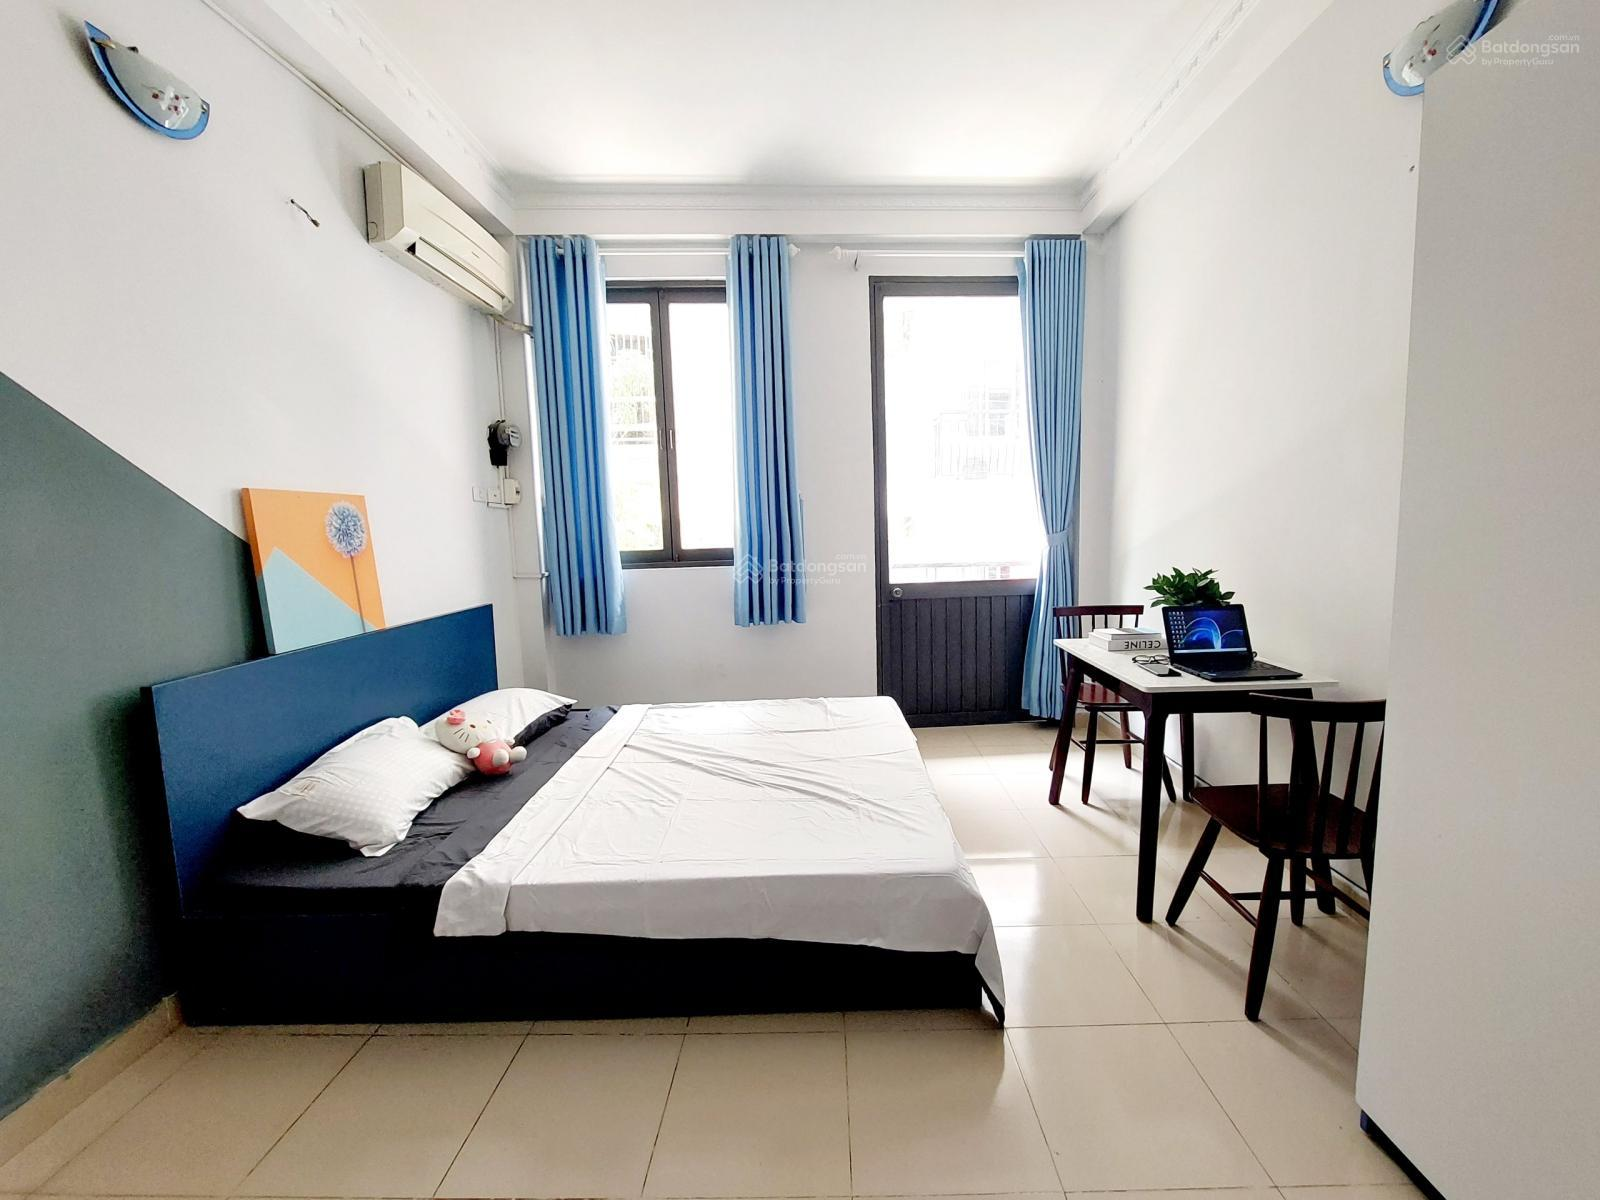
\includegraphics[width=0.7\textwidth]{Images/Overview/PhongTro.jpg}
    \caption{Một phòng trọ cho thuê tại phường Đa Kao, Quận 1, TP.HCM}
\end{figure}
\begin{figure}[H]
    \centering
    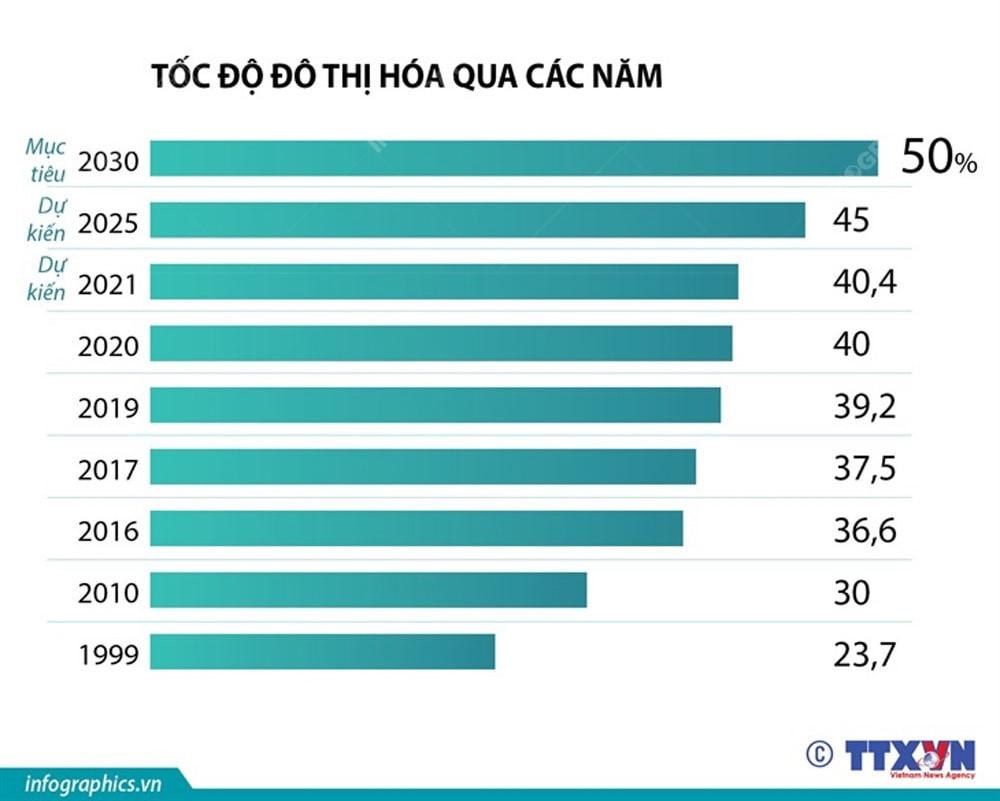
\includegraphics[width=0.6\textwidth]{Images/Overview/TocDoDoThiHoa.jpg}
    \caption{Tốc độ đô thị hóa tại Việt Nam trong 30 năm qua (Nguồn: TTXVN)}
\end{figure}
\begin{figure}[H]
    \centering
    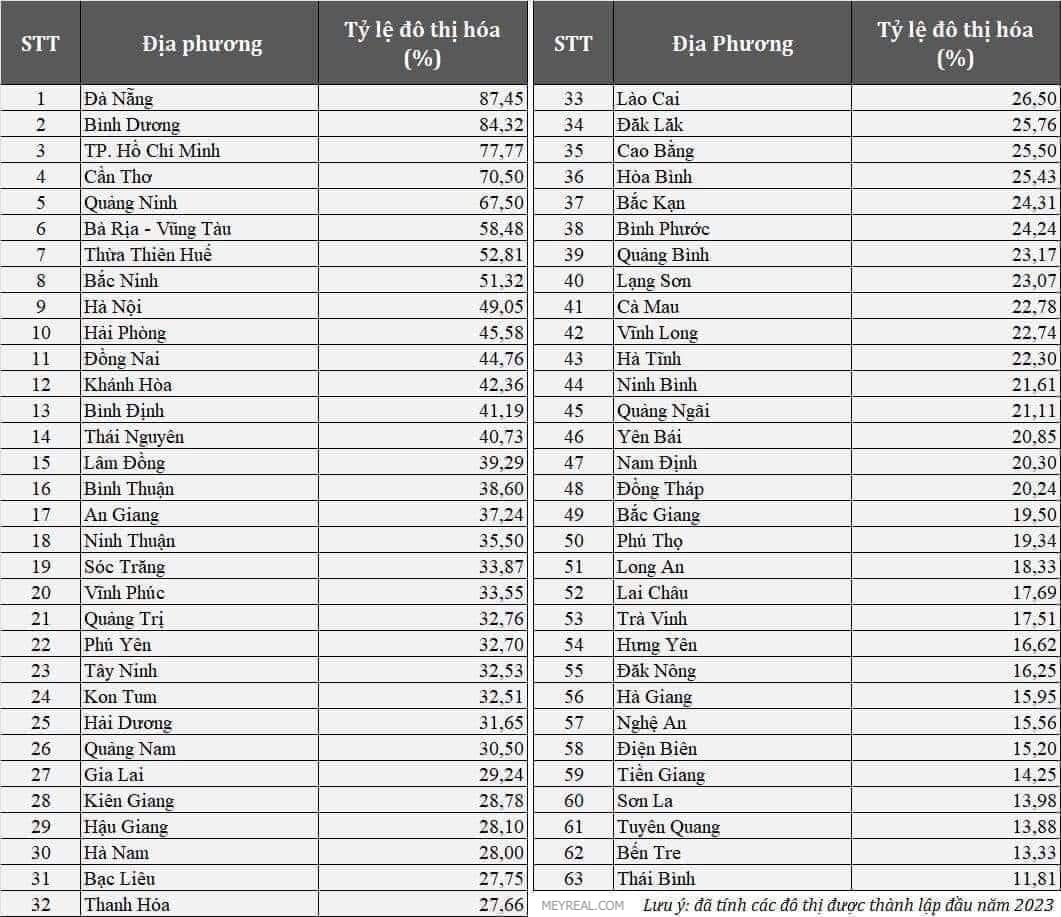
\includegraphics[width=0.95\textwidth]{Images/Overview/TyLeDoThiHoa.jpg}
    \caption{Tỷ lệ đô thị hóa tại các tỉnh thành ở Việt Nam đầu năm 2023 (Nguồn: Kavi Group)}
\end{figure}
\hspace*{1cm} Dựa trên thông tin từ Báo Phụ Nữ \cite{phunu} và Kinh Tế Môi Trường \cite{ktmt}, năm 2022 đã chứng kiến sự phát triển vượt bậc của thị trường nhà trọ tại Việt Nam. Cụ thể, sau một quý I/2022 với mức tăng trưởng ấn tượng, quý II/2022 tiếp tục ghi nhận sự tăng nhẹ trong nguồn cung phòng trọ với mức tăng gần 2\%. Tại TPHCM và tỉnh Bình Dương, mức tăng lần lượt đạt 4,5\% và 12,8\%. Trong khi đó, nguồn cung phòng trọ tại Hà Nội và Đà Nẵng lại giảm lần lượt với tỉ lệ là 10\% và 5,5\%. Nhu cầu thuê nhà trọ, đặc biệt là tại các khu vực lân cận các trường đại học ở TPHCM và Hà Nội, đã tăng mạnh trong năm 2022. Điều này là do quá trình nhập học của năm 2022 đã trở lại bình thường sau một thời gian dài bị ảnh hưởng bởi dịch COVID-19, và một lượng lớn sinh viên mới sẽ cần tìm chỗ ở để phục vụ quá trình học tập tại các thành phố lớn.ẽ có nhu cầu tìm chỗ ở phục vụ quá trình học tập tại các thành phố lớn.
Nhu cầu thuê trọ của các đối tượng cư dân đô thị rất đa dạng, bao gồm:
\begin{itemize}
    \item \textit{Sinh viên:} Sinh viên là đối tượng có nhu cầu thuê trọ cao nhất tại các thành phố lớn. Theo thống kê của Bộ Giáo dục và Đào tạo, tính đến năm 2022, cả nước có khoảng 10 triệu sinh viên, trong đó có khoảng 4 triệu sinh viên đang theo học tại các trường đại học, cao đẳng ở TPHCM và Hà Nội.
    \item \textit{Công nhân:} Công nhân cũng là một đối tượng có nhu cầu thuê trọ cao tại các thành phố lớn. Theo thống kê của Tổng cục Thống kê, tính đến năm 2022, cả nước có khoảng 15 triệu lao động làm việc trong các khu công nghiệp, trong đó có khoảng 5 triệu lao động đang làm việc tại các khu công nghiệp ở TPHCM và Hà Nội.
    \item \textit{Người dân:} Ngoài sinh viên và công nhân, còn có một số đối tượng khác cũng có nhu cầu thuê trọ, chẳng hạn như người lao động tự do, người về hưu,...
\end{itemize}
Trong thời đại số hóa, việc sử dụng điện thoại thông minh để tìm kiếm, đăng tin và quản lý nhà trọ đã trở thành một phần không thể thiếu và tiện lợi. smartphone, với sự đa dạng về chức năng và ứng dụng, đã trở thành thiết bị di động phổ biến nhất hiện nay. Theo VTV, vào năm 2022, số lượng người dùng điện thoại thông minh trên toàn cầu ước tính đạt 6,6 tỷ người, tăng 4,9\% hàng năm \cite{smartphone2022}. Tại Việt Nam, theo Chiến lược hạ tầng số quốc gia đến năm 2025, mục tiêu là 85\% người trưởng thành sẽ sở hữu điện thoại thông minh \cite{chienluoc}. Đại diện Cục Viễn thông (Bộ Thông tin và Truyền thông) cho biết, vào cuối năm 2021, Việt Nam đã có 91,3 triệu thuê bao điện thoại thông minh \cite{vnsmartphone}.
\begin{figure}[h]
    \centering
    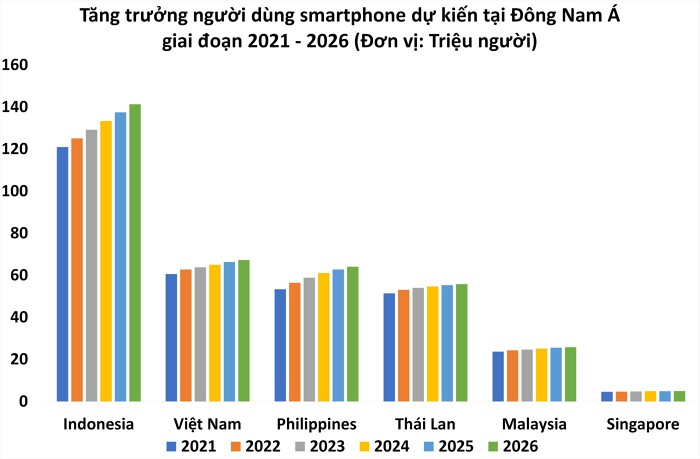
\includegraphics[width=1\textwidth]{Images/Overview/TangTruongSmartphone.jpg}
    \caption{Tăng trưởng người dùng smartphone tại Đông Nam Á giai đoạn 2021 - 2026 (Nguồn: VietnamBiz)}
\end{figure}
Với sự phát triển của công nghệ thông tin, các chủ kinh doanh nhà trọ đã bắt đầu sử dụng các nền tảng mạng xã hội như Facebook, Zalo,... để quảng bá nhà trọ của mình. Tuy nhiên, cách thức quảng bá này vẫn còn tồn tại một số bất cập, cụ thể như sau:
\begin{itemize}
    \item \textit{Phạm vi tiếp cận hạn chế:} Các nền tảng mạng xã hội có lượng người dùng đông đảo, nhưng không phải tất cả những người dùng này đều có nhu cầu thuê nhà trọ. Do đó, việc quảng bá nhà trọ trên các nền tảng mạng xã hội sẽ khiến cho thông tin nhà trọ tiếp cận được với một số lượng người dùng hạn chế.
    \item \textit{Thông tin không được phân loại:} Thông tin nhà trọ được đăng tải trên các nền tảng mạng xã hội thường không được phân loại theo các tiêu chí như vị trí, giá cả, tiện ích,... Điều này khiến cho người thuê trọ khó có thể tìm kiếm được nhà trọ phù hợp với nhu cầu của mình. 
    \item \textit{Tính cạnh tranh cao:} Trên các nền tảng mạng xã hội, có rất nhiều thông tin nhà trọ được đăng tải. Điều này khiến cho thông tin nhà trọ của các chủ kinh doanh nhà trọ dễ bị \textit{"chìm"} và không được người thuê trọ chú ý.
\end{itemize}
Tương tự như trên, với sự phát triển của công nghệ thông tin, việc tìm kiếm nhà trọ đã trở nên dễ dàng hơn bao giờ hết. Tuy nhiên, bên cạnh những lợi ích, việc tìm kiếm nhà trọ qua các nền tảng công nghệ thông tin cũng tồn tại một số bất cập, cụ thể như sau:
\begin{itemize}
    \item \textit{Thiếu thông tin chính xác:} Thông tin nhà trọ được đăng tải trên các nền tảng công nghệ thông tin thường chỉ bao gồm những thông tin cơ bản như diện tích, giá cả, vị trí,... Điều này khiến cho người thuê trọ khó có thể đánh giá được chất lượng thực tế của nhà trọ. Ngoài ra, một số trường hợp chủ kinh doanh nhà trọ cố tình đăng tải thông tin nhà trọ không chính xác để thu hút khách hàng.
    \item \textit{Khó khăn để tìm kiếm nhà trọ phù hợp:} Các nền tảng công nghệ thông tin có lượng thông tin nhà trọ rất lớn, nhưng không được phân loại theo các tiêu chí như vị trí, giá cả, tiện ích,... Điều này khiến cho người thuê trọ khó có thể tìm kiếm được nhà trọ phù hợp với nhu cầu của mình.
    \item \textit{Tốn thời gian và công sức:} Để tìm được nhà trọ phù hợp, người thuê trọ thường phải mất nhiều thời gian để tìm kiếm thông tin trên các nền tảng công nghệ thông tin. Ngoài ra, người thuê trọ cũng phải gặp gỡ trực tiếp chủ kinh doanh nhà trọ để xem xét nhà trọ trước khi quyết định thuê.
\end{itemize}
Trước bối cảnh gia tăng nhu cầu về phòng trọ, sự phát triển của smartphone cũng như nhìn nhận ra những vấn đề mà người chủ trọ cũng như người thuê trọ có thể gặp phải trong việc đăng tải và tìm thuê nhà trọ, nhóm nghiên cứu muốn hướng đến một giải pháp tìm kiếm nhà trọ thông minh trên thiết bị di động, nhằm tạo ra sự tiện lợi và nhanh chóng trong việc kết nối giữa chủ trọ và người thuê.
\section{MỤC ĐÍCH ĐỀ TÀI}
Nhóm thực hiện đề tài mong muốn cung cấp một giải pháp ứng dụng để giải quyết được những bất cập nêu trên. Thông qua việc xây dựng một hệ thống kết nối và tìm kiếm nhà trọ trên nền tảng nhà trọ thông minh, nhóm sẽ mang lại cho cả chủ trọ và người thuê trọ những tiện ích sau:
\begin{itemize}
    \item Tiết kiệm thời gian: Người thuê có thể dễ dàng tìm kiếm và so sánh các nhà trọ phù hợp với nhu cầu của bản thân. Trong khi đó, chủ trọ có thể đăng bài về nhà trọ một cách nhanh chóng và dễ dàng tiếp cận đến với mọi người.
    \item Cung cấp thông tin đầy đủ và chính xác: Các thông tin nhà trọ được số hóa, dễ dàng chỉnh sửa khi có thay đổi tiện ích hoặc giá cả.
    \item Kết nối cộng đồng người thuê rộng rãi: Những người dùng đã từng thuê hoặc đang thuê có thể để lại những đánh giá về nhà trọ, giúp cho những người dùng đang có dự định thuê sẽ nắm rõ hơn về thực trạng hiện tại cũng như những lưu ý liên quan đến nhà trọ đó.
\end{itemize}
\section{MỤC TIÊU ĐỀ TÀI}
Thông qua việc lên kế hoạch và thực hiện đề tài, nhóm muốn sẽ đạt được các mục tiêu như sau:
\begin{itemize}
    \item Hiện thực được các chức năng quan trọng, cấp thiết của ứng dụng như tạo nhà trọ, đăng nhà trọ và đặc biệt là tính năng tìm kiếm nhà trọ có thể trả về kết quả chính xác và nhanh chóng.
    \item Xây dựng được mô hình gợi ý nhà trọ hiệu quả, phù hợp với nhu cầu của người dùng.
    \item Triển khai thành công ứng dụng lên các cửa hàng ứng dụng như Google Play và App Store.
\end{itemize}
\section{ĐỐI TƯỢNG \& PHẠM VI NGHIÊN CỨU}
Phạm vi nghiên cứu của đề tài nhằm hỗ trợ các đối tượng sử dụng ứng dụng tìm thuê nhà trọ tại Việt Nam trong đó bao gồm các nhóm và cá nhân sau:\\
\textbf{Người thuê nhà:}
\begin{itemize}
    \item Sinh viên: sinh viên đến từ các tính lên các thành phố lớn muốn tìm chỗ thuê trọ  trong các khu vực gần trường đại học hoặc cao đẳng.
    \item Người lao động mới: Các người đi làm mới đến một thành phố có thể là đối tượng quan trọng, đặc biệt là những người cần tìm nhà ổn định trong khoảng thời gian ngắn.
\end{itemize}
\textbf{Chủ nhà trọ:}
\begin{itemize}
    \item Chủ nhà nhỏ: Những người sở hữu một số ít phòng trọ và muốn quảng bá cho việc cho thuê chỗ ở của họ.
    \item Doanh nghiệp quản lý nhà trọ: Các công ty hoặc tổ chức quản lý nhiều căn hộ hoặc phòng trọ có thể quan tâm đến cách tối ưu hóa quá trình cho thuê và giữ chỗ ở , cũng như tham khảo giá cá trị trường để tăng tính cạnh tranh trong lĩnh vực cho thuê nhà trọ.
\end{itemize}
Ứng dụng được phát triển trên nền tảng thiết bị di động với ứng dụng bao gồm giao diện có thể tương tác của các chức năng chính và các yêu cầu phi chức năng sẽ được phát triển đầy đủ. Công cụ tìm kiếm với tính năng cho phép người dùng mô tả thông tin về nhà trọ mà người thuê trọ mong muốn cũng sẽ được nghiên cứu và hiện thực
\section{PHƯƠNG PHÁP NGHIÊN CỨU}
Để có được hướng đi đúng đắn cho đề tài lần này, cả nhóm sẽ sử dụng các phương pháp sau để có được cái nhìn chi tiết hơn, đồng thời rút ra điểm cốt lõi để phát triển dự án
\begin{enumerate}
    \item \textbf{Phương pháp phân tích \& tổng hợp :} Phương pháp này tập trung vào việc phân tích và tổng hợp thông tin liên quan đến ứng dụng tìm kiếm nhà trọ. Đây là bước đầu tiên trong quá trình nghiên cứu, trong đó ta thu thập và phân tích các thông tin về nhu cầu của người dùng, tính năng cần có của ứng dụng, các yếu tố liên quan đến nhà trọ (ví dụ: vị trí, giá cả, tiện ích,...) và các ứng dụng tìm kiếm nhà trọ hiện có trên thị trường. Sau đó, các thông tin này được tổng hợp để xác định các yêu cầu cụ thể cho ứng dụng tìm kiếm nhà trọ.
    \item \textbf{Phương pháp thực nghiệm :} Phương pháp thực nghiệm tập trung vào việc triển khai thực hiện các thí nghiệm hoặc các bài toán thực tế để xác minh tính khả thi và hiệu quả của ứng dụng tìm kiếm nhà trọ. Trong trường hợp này, có thể xây dựng một phiên bản mẫu của ứng dụng và thử nghiệm chức năng, hiệu suất và trải nghiệm người dùng của nó. Các phản hồi từ người dùng và dữ liệu thu thập được trong quá trình thực nghiệm sẽ giúp cải thiện và điều chỉnh ứng dụng.
    \item \textbf{Phướng pháp so sánh :} Giúp chỉ ra ưu nhược điểm của ứng dụng tìm kiếm nhà trọ so với các ứng dụng tương tự trên thị trường. Bằng cách nghiên cứu và so sánh các tính năng, giao diện, hiệu suất, độ tin cậy và các yếu tố khác, ta có thể đánh giá được điểm mạnh và điểm yếu của ứng dụng tìm kiếm nhà trọ, từ đó tìm cách cải thiện nó để nâng cao sự cạnh tranh, hoàn thiện của ứng dụng.
    \item \textbf{Phương pháp liệt kê :} Tập trung vào việc liệt kê và phân tích các yếu tố cần có trong ứng dụng tìm kiếm nhà trọ. Các yếu tố này có thể bao gồm: tính năng tìm kiếm bằng cách mô tả, tìm kiếm thông qua các tiện ích, khu vực, thông tin chi tiết về nhà trọ, đánh giá từ người dùng, tiện ích xung quanh, quản lý giao dịch và các tính năng khác. Qua việc liệt kê và phân tích các yếu tố này, ta có thể hiểu rõ hơn về các thành phần và chức năng cần có trong ứng dụng tìm kiếm nhà trọ.
\end{enumerate}
\chapter{KIẾN THỨC NỀN TẢNG}
\section{BÀI TOÁN TÌM KIẾM}
\hspace*{1cm}Bài toán tìm kiếm là một trong những vấn đề quan trọng và phổ biến nhất trong lĩnh vực khoa học máy tính và công nghệ thông tin, đặc biệt là trong việc phát triển các ứng dụng di động và web. Bài toán này liên quan đến việc xác định cách thức để tìm kiếm thông tin từ một tập dữ liệu lớn dựa trên các yêu cầu cụ thể của người dùng hiệu quả và chính xác nhất. Đối với nền tảng nhà trọ thông minh, bài toán tìm kiếm có vai trò quyết định trong việc giúp người dùng tìm thấy nhà trọ phù hợp nhanh chóng và tiện lợi.\\
\hspace*{1cm}Bên cạnh đó, bài toán tìm kiếm tồn tại một số thách thức quan trọng mà cần được vượt qua để xây dựng một hệ thống tìm kiếm hiệu quả và đáp ứng được nhu cầu của người dùng:
\begin{itemize}
    \item Khối lượng dữ liệu lớn: Khi dữ liệu về các nhà trọ rất lớn, việc tìm kiếm nhanh chóng và hiệu quả trở nên khó khăn.
    \item Đa dạng thông tin: Các nhà trọ có thể có nhiều thuộc tính khác nhau, từ vị trí, giá cả, đến các tiện ích đi kèm, làm phức tạp hóa việc so khớp và xếp hạng.
    \item Truy vấn phức tạp: Người dùng có thể đưa ra các truy vấn phức tạp, đòi hỏi hệ thống phải hiểu và xử lý chính xác các điều kiện kết hợp.
    \item Độ chính xác: Đảm bảo rằng các kết quả trả về phải chính xác và phù hợp với mong đợi của người dùng.
    \item Hiệu suất: Duy trì hiệu suất cao trong việc xử lý truy vấn và trả kết quả trong thời gian ngắn.
\end{itemize}

\hspace*{1cm}Để có thể vượt qua những thách thức, việc xây dựng một mô hình tìm kiếm đòi hỏi phải có sự kết hợp giữa các kỹ thuật xử lý dữ liệu lớn, tối ưu hóa cơ sở dữ liệu, và áp dụng các thuật toán tìm kiếm và xếp hạng hiệu quả. Đồng thời, việc nắm bắt và hiểu rõ nhu cầu của người dùng cũng là chìa khóa để xây dựng một hệ thống tìm kiếm nhà trọ thành công và đáp ứng được mọi yêu cầu.
\section{TÌM KIẾM TOÀN VĂN BẢN}
\subsection{Tổng quan}
\hspace*{1cm}Tìm kiếm toàn văn bản là một phương pháp tìm kiếm thông tin trong toàn bộ nội dung của một văn bản, thay vì chỉ tìm kiếm trong tiêu đề, tóm tắt hoặc các trường chỉ mục. Điểm khác biệt giữa Tìm kiếm toàn văn bản và các kĩ thuật tìm kiếm thông thường khác là \textbf{Inverted Index}. Inverted Index là kĩ thuật tìm kiếm index theo đơn vị term thay vì index theo đơn vị row. Cụ thể hơn, Inverted Index giúp ánh xạ từ khóa tìm kiếm với các vị trí (hoặc các tài liệu) mà từ khóa đó xuất hiện. \\
Ví dụ như ở Hình \ref{fig:ftsexample}, term "new" nằm trong các document 4, 5 và 8 do đó sẽ được đánh index là 4,5,8. Việc sử dụng Inverted Index giúp cho tìm kiếm toàn văn bản trên database trở nên nhanh hơn bao giờ hết. Giả sử khi chúng ta muốn query cụm từ "Your first car", thay vì việc phải scan trên từng document một để tìm ra kết quả, bài toán tìm kiếm document chứa 3 term trên sẽ trở thành phép toán union của 3 tập hợp (document sets) của 3 term đó trong Inverted Index.\\
        \[
result = \{2,9\} \cup \{9\} \cup \{4\}
\]
\begin{figure}[H]
    \centering
    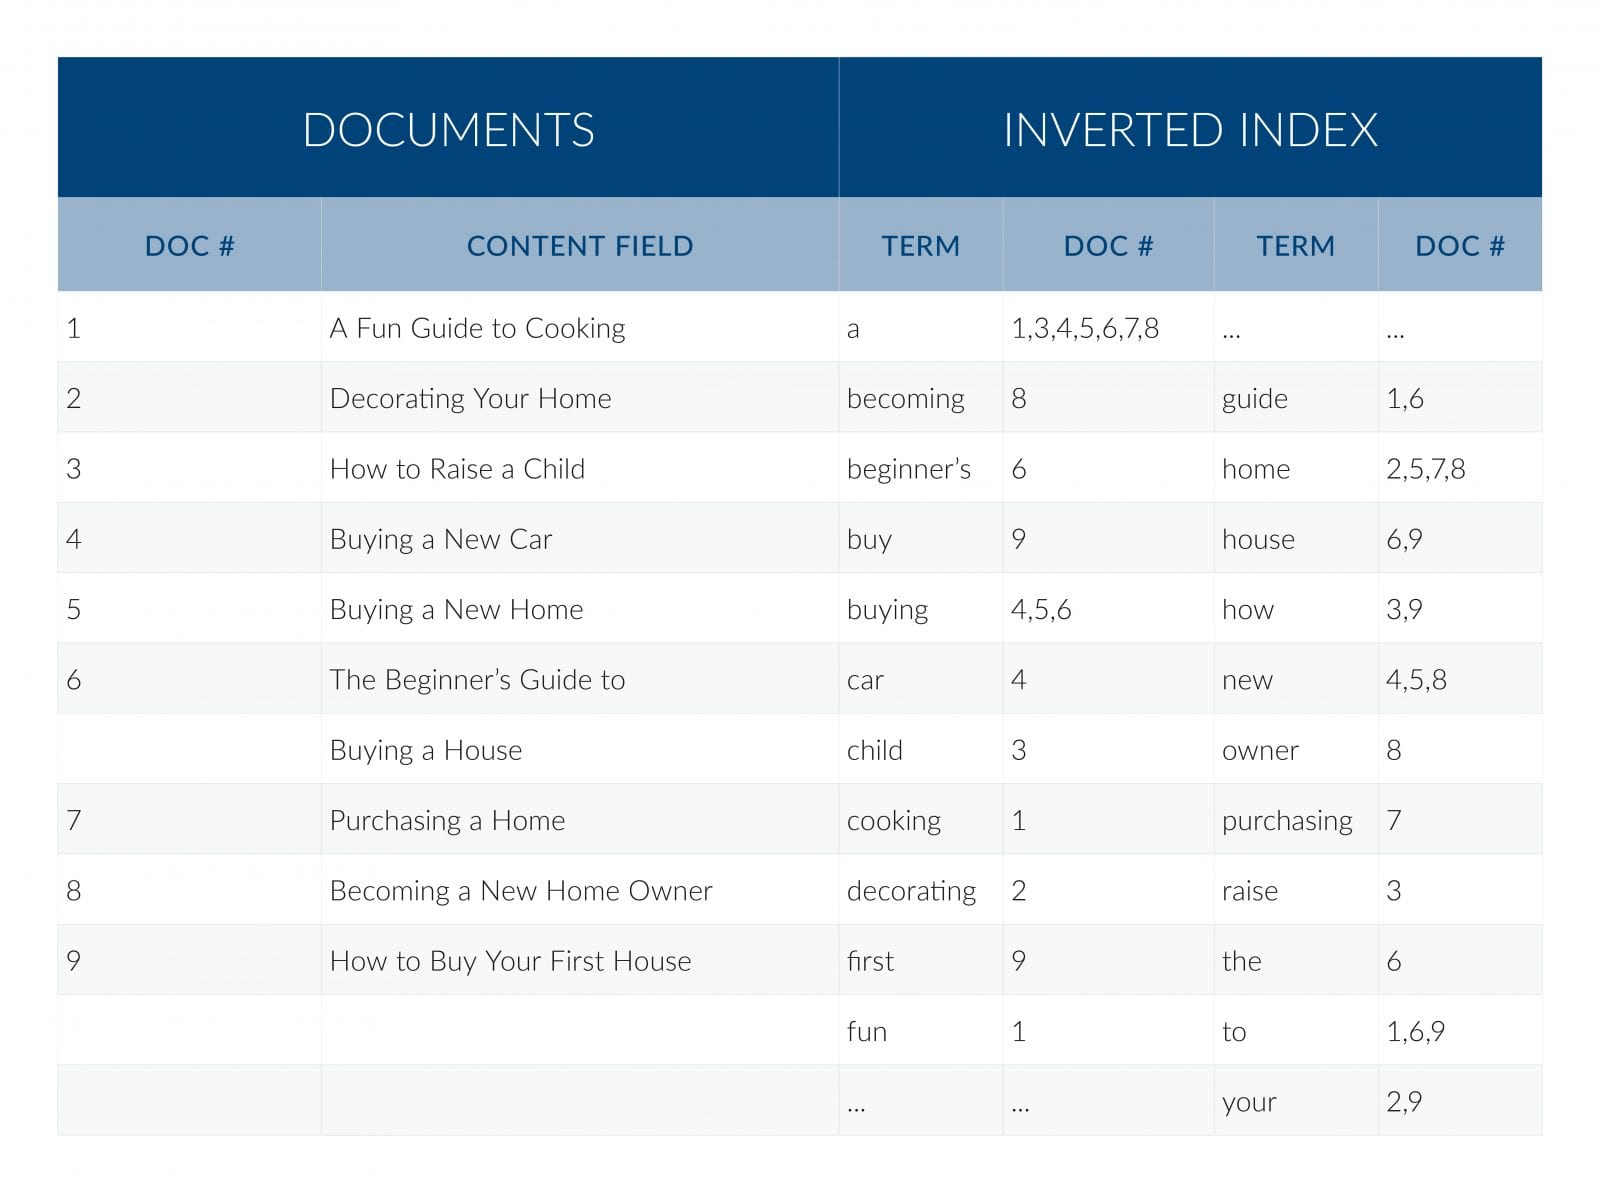
\includegraphics[width=1\textwidth]{Images/HybridSearch/FullTextSearch.png}
    \caption{Document và Term trong tìm kiếm toàn văn bản}
    \label{fig:ftsexample}
\end{figure}

\subsection{Phân tích ưu và nhược điểm}
\textbf{Ưu điểm}
\begin{itemize}
    \item \textbf{Tìm kiếm nhanh chóng và dễ dàng:} giúp tìm kiếm thông tin nhanh chóng và dễ dàng hơn, vì người dùng không cần phải biết chính xác vị trí của thông tin trong văn bản.
    \item \textbf{Có thể tìm kiếm thông tin phi cấu trúc:} có thể tìm kiếm thông tin phi cấu trúc, chẳng hạn như email, tin nhắn và tài liệu mạng xã hội.
    \item \textbf{Cải thiện trải nghiệm người dùng:} tìm kiếm thông tin hiệu quả hơn và tiết kiệm thời gian.
\end{itemize}
\textbf{Nhược điểm}
\begin{itemize}
    \item \textbf{Yêu cầu nhiều dung lượng lưu trữ:} đòi hỏi phải lưu trữ nhiều dữ liệu hơn các phương pháp tìm kiếm truyền thống, do đó nó có thể tốn kém hơn.
    \item \textbf{Kết quả có thể không chính xác hoàn toàn:} Mặc dù đã được cải tiến rất nhiều, nhưng nó vẫn có thể trả về những kết quả không chính xác hoàn toàn.
    \item \textbf{Chưa giải quyết được vấn đề từ đồng nghĩa:} Ngôn ngữ nào cũng sẽ có các từ đồng nghĩa do vậy không thể đảm bảo sẽ có thể trả về kết quả như mong muốn khi gặp phải từ đồng nghĩa
\end{itemize}
\section{TÌM KIẾM NGỮ NGHĨA}
\subsection{Tổng quan}
\hspace*{1cm}Tìm kiếm ngữ nghĩa là một công cụ search thông qua việc phân tích các từ ngữ và các cụm từ, trả về kết quả có nội dung các từ tương đồng với ngữ nghĩa các từ khóa xuất hiện trong câu truy vấn thay vì phải trùng khớp từng từ, sử dụng trí tuệ nhân tạo để hiểu ý nghĩa của truy vấn và mối quan hệ giữa các từ để trả về những kết quả phù hợp và chính xác hơn.\\
\hspace*{1cm}Tìm kiếm ngữ nghĩa được vận hành dựa trên vector search cho phép semantic search để có thể tìm kiếm và sắp xếp thông tin dựa trên các nội dung liên quan. Vector search mã hóa các chi tiết của thông tin tìm kiếm thành các trường có liên quan hoặc các vector để có thể so sánh các vector và tìm kiếm sự tương đồng giữa chúng
\begin{enumerate}
    \item Khi một câu truy vấn được thực hiện, search engine chuyển câu query thành dạng embedding, đại diện bởi dạng dữ liệu số và các nội dung liên quan, lưu trữ vào các vector.
    \begin{figure}[H]
        \centering
        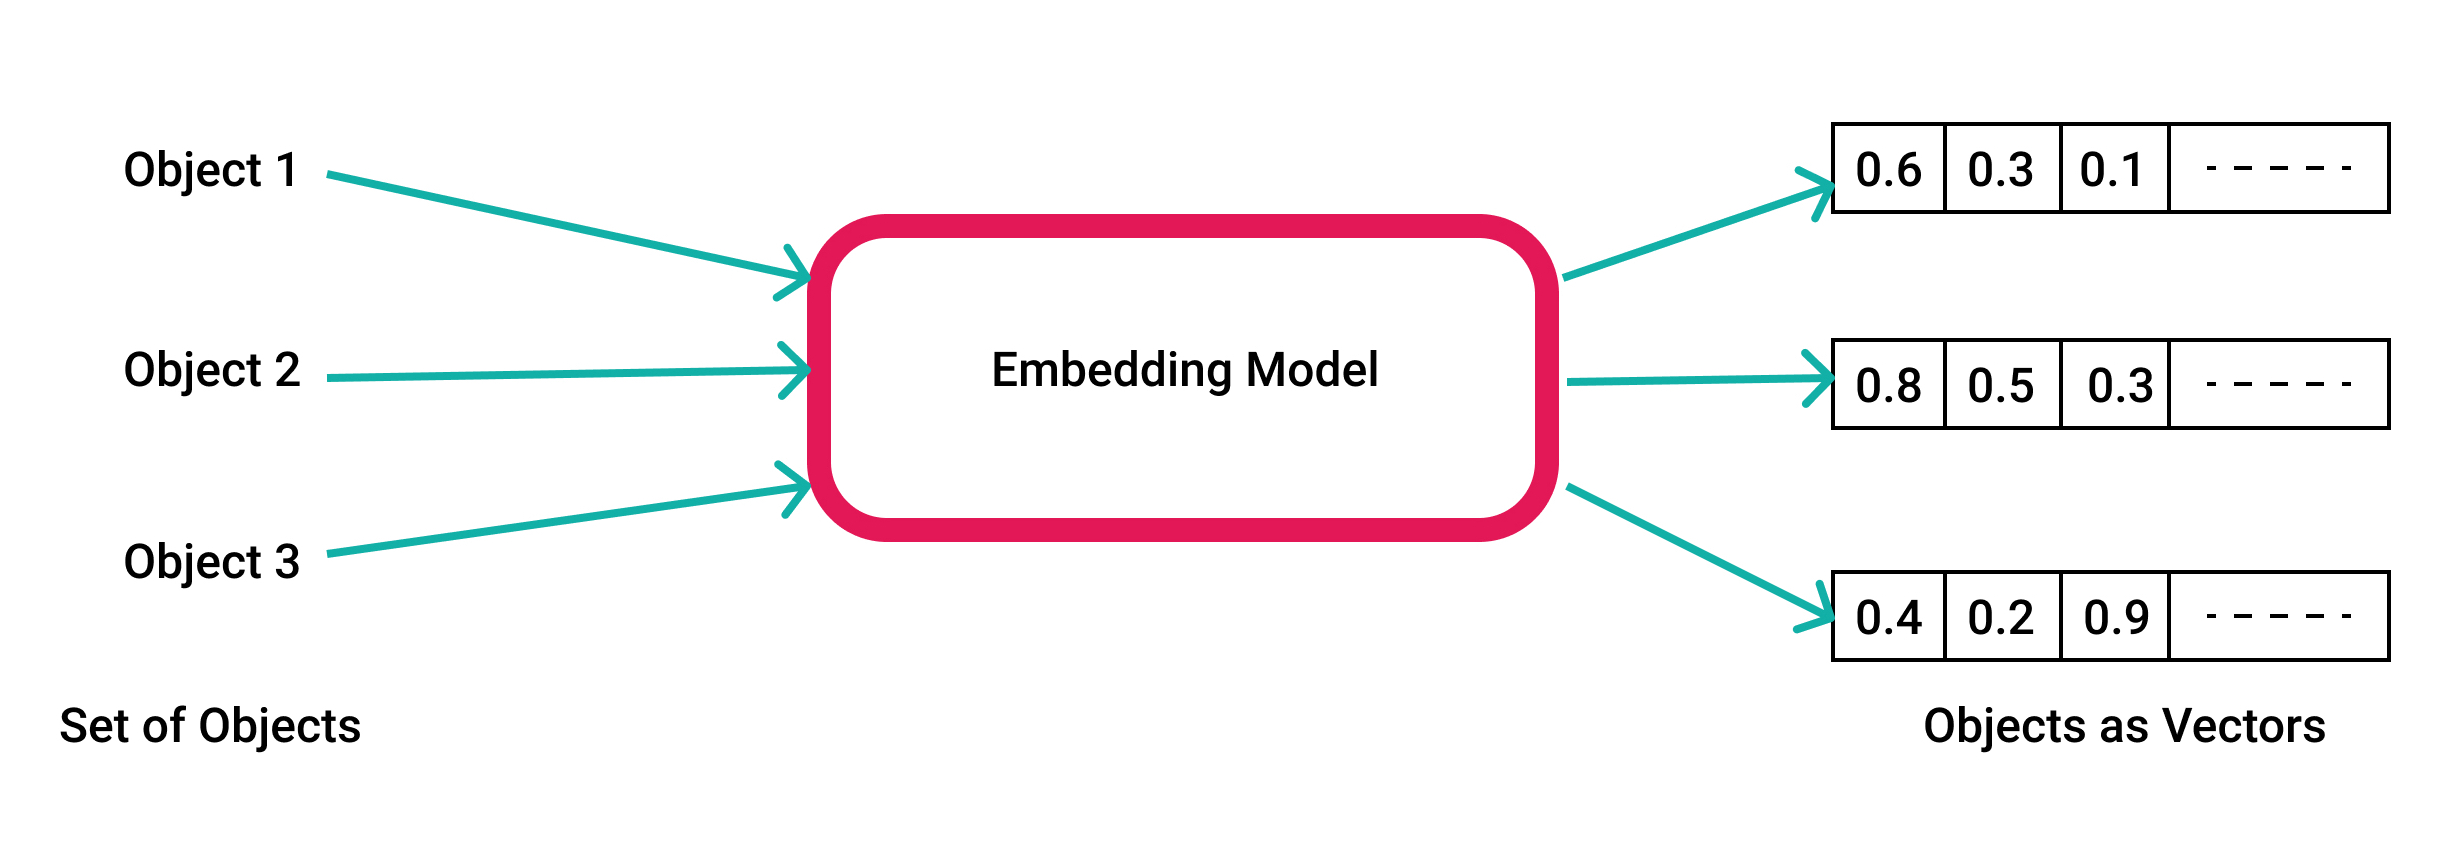
\includegraphics[width=1\textwidth]{Images/embedding.png}
        \caption{Vector embedding}
        \label{fig:ftsexample}
    \end{figure}
    \item Sử dụng Cosine Similarity để tìm các vector chứa các nội dung liên quan đến vector câu truy vấn.
\end{enumerate}
\textbf{Ví dụ:} khi bạn sử dụng tìm kiếm ngữ nghĩa để tìm kiếm "\textbf{nhà hàng gần đây}", nó sẽ không chỉ trả về danh sách các nhà hàng có chứa từ khóa "\textbf{nhà hàng}" và "\textbf{gần đây}", mà còn xem xét các yếu tố khác như vị trí hiện tại, loại nhà hàng bạn thích, và đánh giá của khách hàng.
\subsection{Phân tích ưu và nhược điểm}
\textbf{Ưu điểm}
\begin{itemize}
    \item \textbf{Kết quả chính xác hơn:} giúp người dùng tìm thấy thông tin phù hợp với nhu cầu hơn, vì nó xem xét ý nghĩa và ngữ cảnh của truy vấn.
    \item \textbf{Có thể tìm kiếm thông tin phức tạp:} có thể hiểu được các truy vấn phức tạp và trả về những kết quả phù hợp.
    \item \textbf{Ít phụ thuộc vào từ khóa:} Không cần phải sử dụng những từ khóa chính xác để tìm kiếm thông tin. Thay vào đó, có thể sử dụng ngôn ngữ tự nhiên để diễn đạt truy vấn của mình.
\end{itemize}
\textbf{Nhược điểm}
\begin{itemize}
    \item \textbf{Yêu cầu công nghệ cao:} đòi hỏi phải có công nghệ trí tuệ nhân tạo, học máy để việc tìm kiếm hiệu quả hơn, do đó có thể khá tốn kém và khó khăn để triển khai.
    \item \textbf{Kết quả có thể không chính xác hoàn toàn:} Mặc dù đã được cải tiến rất nhiều, nhưng nó vẫn có thể trả về những kết quả không chính xác hoàn toàn điều này phụ thuộc rất nhiều vào độ chính xác của các mô hình được sử dụng
    \item \textbf{Thiếu dữ liệu:} hoạt động hiệu quả nhất khi có nhiều dữ liệu để phân tích. Nếu không có đủ dữ liệu, có thể không hiểu được ý nghĩa của truy vấn và trả về những kết quả không chính xác.
\end{itemize}
\chapter{KHẢO SÁT CÁC GIẢI PHÁP LIÊN QUAN}
\section{CÁC GIẢI PHÁP TÌM KIẾM TƯƠNG TỰ}
\hspace*{1cm}Ngày nay, nhu cầu tìm kiếm thông tin ngày càng tăng cao, đặc biệt là trong kỷ nguyên internet và dữ liệu bùng nổ. Tuy nhiên, các phương pháp tìm kiếm truyền thống như tìm kiếm theo từ khóa đơn giản thường gặp nhiều hạn chế, dẫn đến kết quả không chính xác, không liên quan và thiếu hiệu quả. Để giải quyết những vấn đề này, các giải pháp tìm kiếm hybrid được ra đời như một hướng tiếp cận tiên tiến, kết hợp các ưu điểm của nhiều phương pháp tìm kiếm khác nhau nhằm nâng cao độ chính xác, tính liên quan và hiệu quả của kết quả tìm kiếm. 
\hspace*{1cm} Chẳng hạn như Yinglong và các cộng sự (2008) \cite{4709221} đã nghiên cứu một mô hình hybrid giúp truy vấn ngữ nghĩa theo cách phân tán. Ngoài ra bài báo còn giới thiệu về việc sắp xếp thứ tự cho các kết quả từ nhiều nguồn bằng cách xếp hạng linh hoạt dựa trên sự chồng chéo của ngữ nghĩa. Mặt khác, Bhagdev và các cộng sự (2008) \cite{inproceedings} đã giới thiệu về K-search, một thuật toán tìm kiếm hybrid dựa trên ontology và so khớp từ khóa.
\section{CÁC ỨNG DỤNG TƯƠNG TỰ}
\subsection{AIRBNB}
\subsubsection{Giới thiệu}
\hspace*{1cm}Airbnb là viết tắt của cụm từ AirBed and Breakfast, là nền tảng mà hàng triệu người dùng trên khắp thế giới tin dùng để tìm kiếm chỗ ở độc đáo và cá nhân. Từ căn hộ hiện đại, nhà nghỉ truyền thống, đến những không gian lạ mắt như căn hộ trên cây hay lâu đài cổ, Airbnb mang đến sự đa dạng vô song để đáp ứng mọi nhu cầu và sở thích của du khách. \cite{airbnb}\\
\hspace*{1cm}Một điểm đặc biệt là khả năng trải nghiệm cuộc sống địa phương thông qua Airbnb. Người dùng không chỉ đặt chỗ ở mà còn có cơ hội tham gia vào những trải nghiệm độc đáo, được tổ chức bởi người dân địa phương. Từ tour tham quan đến lớp nấu ăn truyền thống, những trải nghiệm này không chỉ là hành trình du lịch mà còn là cơ hội để tận hưởng và hiểu rõ văn hóa đặc trưng của địa phương. Năm 2013, Airbnb đã đạt cột mốc 9 triệu người dùng, và tới tháng 10 năm 2019, nền tảng đã đạt được mức 2 triệu lượt đăng ký dịch vụ mỗi đêm. Sau khoảng thời gian hồi phục kinh tế từ đại dịch COVID-19, vào quý 4 năm 2021, doanh thu của công ty đã lên mức 1.5 tỷ USD. \cite{airbnbstat}\\
\hspace*{1cm}Đánh giá và nhận xét đóng vai trò quan trọng trong việc xây dựng niềm tin trong cộng đồng Airbnb. Hệ thống này có sự minh bạch cao, giúp du khách lựa chọn chỗ ở dựa trên trải nghiệm thực tế của những người đã từng ở đó. Đồng thời, nó cũng là một phần quan trọng của quá trình xác minh và chất lượng của các chỗ ở trên nền tảng. Airbnb không chỉ là giải pháp tiết kiệm chi phí cho du khách mà còn mang lại cơ hội cho những người có nhà trống kiếm thêm thu nhập. Bằng cách chia sẻ không gian sống của họ, người cho thuê không chỉ mở cửa sổ nhà mình ra thế giới mà còn kết nối với những người mới và chia sẻ câu chuyện đặc biệt của mình.
\begin{figure}[H]
    \centering
    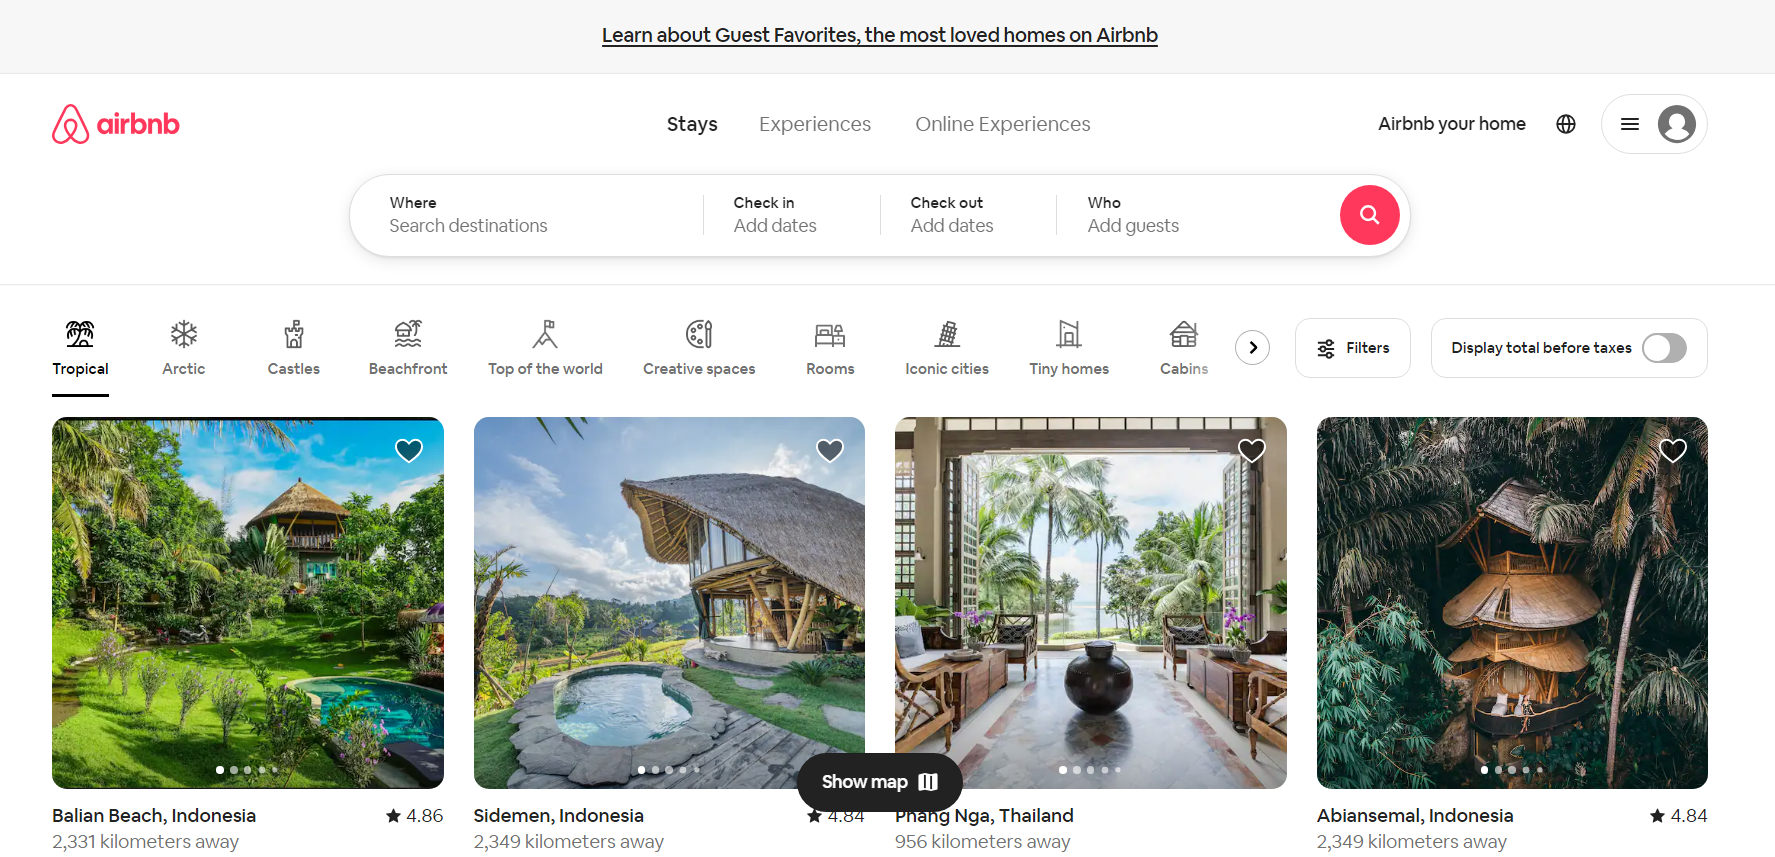
\includegraphics[width=1\textwidth]{Images/RelatedSystems/AirbnbDesktop.png}
    \caption{Giao diện Airbnb trên website}
\end{figure}
\begin{figure}[H]
    \centering
    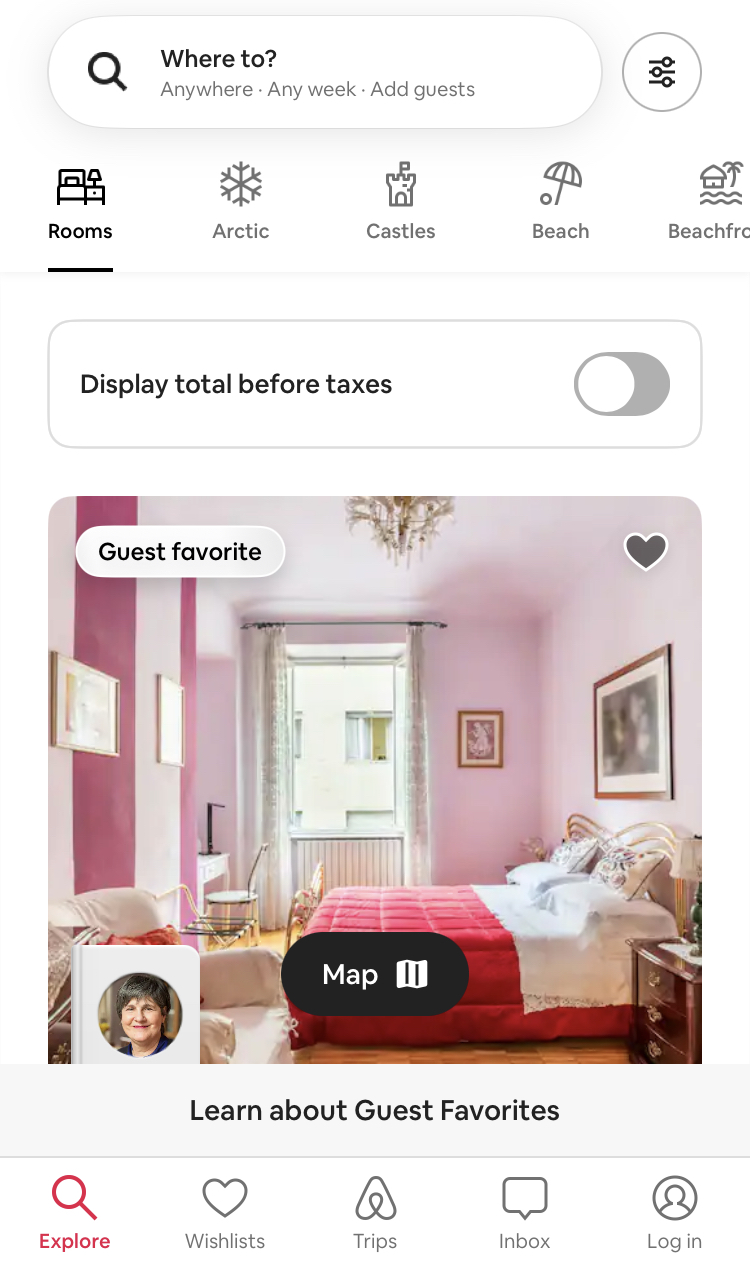
\includegraphics[width=0.5\textwidth]{Images/RelatedSystems/AirbnbMobile.PNG}
    \caption{Giao diện Airbnb trên thiết bị di động}
\end{figure}
\subsubsection{Các tính năng chính}
Airbnb là một nền tảng trực tuyến kết nối người cho thuê nhà/phòng với người tìm nơi ở. Airbnb cung cấp nhiều tính năng khác nhau, bao gồm:
\begin{itemize}
    \item \textbf{Tìm kiếm}
    \begin{itemize}
        \item \textit{Tìm kiếm theo vị trí:} Khách hàng có thể tìm kiếm chỗ ở theo vị trí, chẳng hạn như thành phố, quận, khu phố,...
        \item \textit{Tìm kiếm theo giá cả:} Khách hàng có thể tìm kiếm chỗ ở theo mức giá, chẳng hạn như giá rẻ, giá trung bình, giá cao,...
        \item \textit{Tìm kiếm theo loại chỗ ở:} Khách hàng có thể tìm kiếm chỗ ở theo loại, chẳng hạn như nhà riêng, căn hộ, phòng khách sạn,...
        \item \textit{Tìm kiếm theo tiện nghi:} Khách hàng có thể tìm kiếm chỗ ở có các tiện nghi mong muốn, chẳng hạn như hồ bơi, phòng tập thể dục,...
    \end{itemize}
    \item \textbf{Đặt phòng}
    \begin{itemize}
        \item \textit{Đặt phòng trực tuyến:} Khách hàng có thể đặt phòng chỗ ở trên Airbnb một cách dễ dàng và nhanh chóng.
        \item \textit{Thanh toán linh hoạt:} Airbnb cung cấp nhiều phương thức thanh toán khác nhau để khách hàng lựa chọn, chẳng hạn như thẻ tín dụng, thẻ ghi nợ, PayPal,...
        \item \textit{Hoàn tiền linh hoạt:} Airbnb có chính sách hoàn tiền linh hoạt, giúp khách hàng an tâm khi đặt phòng.
    \end{itemize}
    \item \textbf{Thông tin chỗ ở}
    \begin{itemize}
        \item \textit{Ảnh và video:} Airbnb cung cấp ảnh và video chi tiết về từng chỗ ở, giúp khách hàng có thể hình dung được chỗ ở trước khi đặt phòng.
        \item \textit{Mô tả:} Airbnb cung cấp mô tả chi tiết về từng chỗ ở, bao gồm các thông tin như diện tích, số phòng ngủ, số phòng tắm, tiện nghi,...
        \item \textit{Đánh giá:} Airbnb cung cấp đánh giá của khách hàng đã từng ở chỗ ở, giúp khách hàng có thể đánh giá chất lượng của chỗ ở.
    \end{itemize}
    \item \textbf{Tương tác}
    \begin{itemize}
        \item \textit{Gửi tin nhắn}: Khách hàng có thể gửi tin nhắn cho chủ nhà để trao đổi thông tin, đặt câu hỏi...
        \item \textit{Trao đổi qua Airbnb:} Khách hàng có thể trao đổi với chủ nhà thông qua các công cụ của Airbnb, chẳng hạn như cuộc gọi video, cuộc gọi thoại...
    \end{itemize}
    \item \textbf{Hỗ trợ}
    \begin{itemize}
        \item \textit{Hỗ trợ 24/7:} Airbnb cung cấp dịch vụ hỗ trợ khách hàng 24/7, giúp khách hàng có thể giải quyết các vấn đề trong quá trình sử dụng dịch vụ.
        \item \textit{Trung tâm trợ giúp:} Airbnb cung cấp trung tâm trợ giúp với nhiều tài nguyên hữu ích, giúp khách hàng có thể tự giải quyết các vấn đề.
    \end{itemize}
    \item \textbf{Tính năng bổ sung}
    \begin{itemize}
        \item \textit{Trải nghiệm:} Airbnb cung cấp các trải nghiệm độc đáo, do người dân địa phương tổ chức. Trải nghiệm này giúp khách hàng có thể khám phá văn hóa và con người của địa phương.
        \item \textit{Airbnb for Work:} Airbnb cung cấp các dịch vụ dành riêng cho doanh nghiệp, chẳng hạn như quản lý chuyến công tác, thanh toán theo nhóm,...
    \end{itemize}
\end{itemize}
Ngoài các tính năng trên, Airbnb còn cung cấp một số tính năng khác, chẳng hạn như:
\begin{itemize}
    \item \textbf{Bảo hiểm:} Airbnb cung cấp bảo hiểm cho khách hàng, giúp khách hàng được bảo vệ trong trường hợp xảy ra sự cố.
    \item \textbf{AirCover:} Airbnb cung cấp tính năng AirCover cho khách hàng, giúp khách hàng được bảo vệ trong trường hợp chỗ ở không như mong đợi.
    \item \textbf{Tính toán thuế:} Airbnb cung cấp tính năng tính toán thuế cho khách hàng, giúp khách hàng có thể dễ dàng tính toán thuế khi đặt phòng.
\end{itemize}
\subsubsection{Phân tích SWOT}
\begin{tcbraster}[raster columns=2, boxrule=0mm, arc=0mm]
\begin{tcolorbox}[equal height group=A, size=fbox, colback=swotS!60, colframe=swotS!80!black, title=\textsc{strengths}]
\begin{itemize}
\item Airbnb là công ty tiên phong trong lĩnh vực kinh tế chia sẻ, tạo ra một mô hình mới cho ngành dịch vụ lưu trú.
\item Airbnb cung cấp chỗ ở với mức giá cạnh tranh hơn so với khách sạn truyền thống, phù hợp với nhu cầu của nhiều đối tượng khách hàng.
\item Tốc độ tăng trưởng ấn tượng trong những năm gần đây, với hàng triệu lượt đặt phòng mỗi đêm trên toàn thế giới.
\item Airbnb có lượng dữ liệu khách hàng khổng lồ, giúp công ty hiểu rõ nhu cầu và hành vi của khách hàng, từ đó cải thiện chất lượng dịch vụ.
\end{itemize}
\end{tcolorbox}
\begin{tcolorbox}[equal height group=A, size=fbox, colback=swotW!60, colframe=swotW!80!black, title=\textsc{weaknesses}]
\begin{itemize}
\item Airbnb không trực tiếp quản lý chất lượng dịch vụ của các chủ nhà, dẫn đến một số trường hợp khách hàng gặp phải chất lượng dịch vụ không như mong đợi.
\item Một số vụ bê bối liên quan đến Airbnb, đã gây ảnh hưởng xấu đến hình ảnh thương hiệu của công ty.
\item Ở một số quốc gia, tính pháp lý của Airbnb vẫn chưa được rõ ràng, dẫn đến những rủi ro cho công ty.
\item Airbnb đang phải đối mặt với sự cạnh tranh ngày càng tăng từ các đối thủ như Booking.com, Expedia,...
\end{itemize}
\end{tcolorbox}
\begin{tcolorbox}[equal height group=B, size=fbox, colback=swotO!60, colframe=swotO!80!black, title=\textsc{opportunities}]
\begin{itemize}
\item Ngành du lịch đang có xu hướng tăng trưởng mạnh mẽ, tạo ra nhiều cơ hội cho Airbnb.
\item Sự phát triển của công nghệ, chẳng hạn như trí tuệ nhân tạo, sẽ giúp Airbnb cải thiện chất lượng dịch vụ và trải nghiệm của khách hàng.
\item Airbnb có thể mở rộng sang các thị trường mới, chẳng hạn như các thị trường đang phát triển, để tiếp cận nhiều khách hàng hơn.
item Airbnb có thể phát triển các sản phẩm và dịch vụ mới, chẳng hạn như dịch vụ cho thuê xe, dịch vụ ăn uống,... để đáp ứng nhu cầu ngày càng đa dạng của khách hàng.
\end{itemize}
\end{tcolorbox}
\begin{tcolorbox}[equal height group=B, size=fbox, colback=swotT!60, colframe=swotT!80!black, title=\textsc{threats}]
\begin{itemize}
\item Xu hướng du lịch có thể thay đổi theo thời gian, dẫn đến những thách thức cho Airbnb.
\item Sự phát triển của các công nghệ mới, chẳng hạn như thực tế ảo, có thể thay đổi cách thức du lịch của mọi người, dẫn đến những thách thức cho Airbnb.
\item Các quy định và thuế mới có thể ảnh hưởng đến hoạt động kinh doanh của Airbnb.
\item Kinh tế suy thoái có thể dẫn đến giảm nhu cầu du lịch, từ đó ảnh hưởng đến doanh thu của Airbnb.
\end{itemize}
\end{tcolorbox}
\captionof{table}{Phân tích SWOT cho Airbnb}
\end{tcbraster}
\subsubsection{Nhận xét}
\hspace*{1cm}Airbnb, với định dạng đặt phòng trực tuyến độc đáo, đã làm thay đổi bối cảnh của ngành du lịch và góp phần tạo ra một mô hình động mới cho việc tương tác với môi trường địa phương. Nền tảng này không chỉ mang lại sự linh hoạt và đa dạng trong việc lựa chọn chỗ ở, từ những căn hộ hiện đại đến những ngôi nhà truyền thống, mà còn mở ra một cửa sổ rộng lớn để du khách tương tác với văn hóa địa phương một cách chân thực.\\
\hspace*{1cm}Trải nghiệm của du khách trên Airbnb không chỉ là việc tìm kiếm nơi lưu trú, mà còn là việc kết nối với cộng đồng địa phương thông qua việc ở chung với các chủ nhà địa phương. Sự ấm cúng và thuận tiện được cung cấp bởi các chỗ ở này không chỉ giúp tạo ra không gian thoải mái cho du khách mà còn đóng góp vào sự đa dạng và sâu sắc của trải nghiệm du lịch.\\ \hspace*{1cm}Tuy nhiên, trong bối cảnh lớn và đa dạng như vậy, việc quản lý chất lượng và an toàn trở nên quan trọng. Các vấn đề như đánh giá chủ nhà, phản hồi từ cộng đồng, và các biện pháp an ninh cần được xem xét một cách cẩn thận để đảm bảo rằng môi trường Airbnb duy trì một tiêu chuẩn cao về chất lượng dịch vụ và an toàn cho mọi du khách.
\section{BATDONGSAN (PROPERTYGURU)}
\subsection{Giới thiệu}
\hspace*{1cm}Được ra mắt vào năm 2008, trang web Batdongsan.com.vn là một nền tảng hàng đầu tại Việt Nam trong lĩnh vực bất động sản. Với sứ mệnh cung cấp thông tin đầy đủ, chính xác và đa dạng về thị trường nhà đất. Năm 2010, trang web đã trở thành website hàng đầu trong lĩnh vực bất động sản. Vào tháng 10 năm 2018, sau khi chính thức gia nhập tập đoàn PropertyGuru,  PropertyGuru, Batdongsan.com.vn đã vươn lên một cách vượt trội nhờ tận dụng không ngừng lợi thế về công nghệ và dữ liệu từ tập đoàn lớn, từ đó trang web đã thực hiện nhiều cải tiến quan trọng như nâng cấp giao diện, cải thiện tính năng tìm kiếm và tăng tốc độ trải nghiệm. \cite{batdongsan} Batdongsan.com.vn không chỉ là nguồn tin tin cậy cho người mua và người bán mà còn là điểm đến đáng tin cậy cho những ai quan tâm đến thị trường bất động sản.\\
\hspace*{1cm}Batdongsan.com.vn cung cấp một loạt các danh mục bất động sản, từ căn hộ, nhà phố đến đất đai và dự án mới. Người dùng có thể dễ dàng tìm kiếm, so sánh và lựa chọn bất động sản phù hợp với nhu cầu và ước mơ của mình. Điều này giúp tối ưu hóa trải nghiệm người dùng và tiết kiệm thời gian trong quá trình tìm kiếm. Trang web không ngừng cập nhật thông tin về thị trường bất động sản, giúp người dùng có cái nhìn toàn diện về xu hướng giá cả, quy hoạch đô thị, và những dự án nổi bật. Điều này giúp người dùng đưa ra quyết định thông tin và hiệu quả. Ngoài việc cung cấp thông tin, Batdongsan.com.vn còn tạo ra một cộng đồng sôi động, nơi mà người dùng có thể chia sẻ kinh nghiệm, đánh giá về các dự án, và hỗ trợ nhau trong quá trình mua bán bất động sản. Điều này làm cho trang web trở thành điểm đến toàn diện cho mọi người quan tâm đến thị trường bất động sản tại Việt Nam.
\begin{figure}[H]
    \centering
    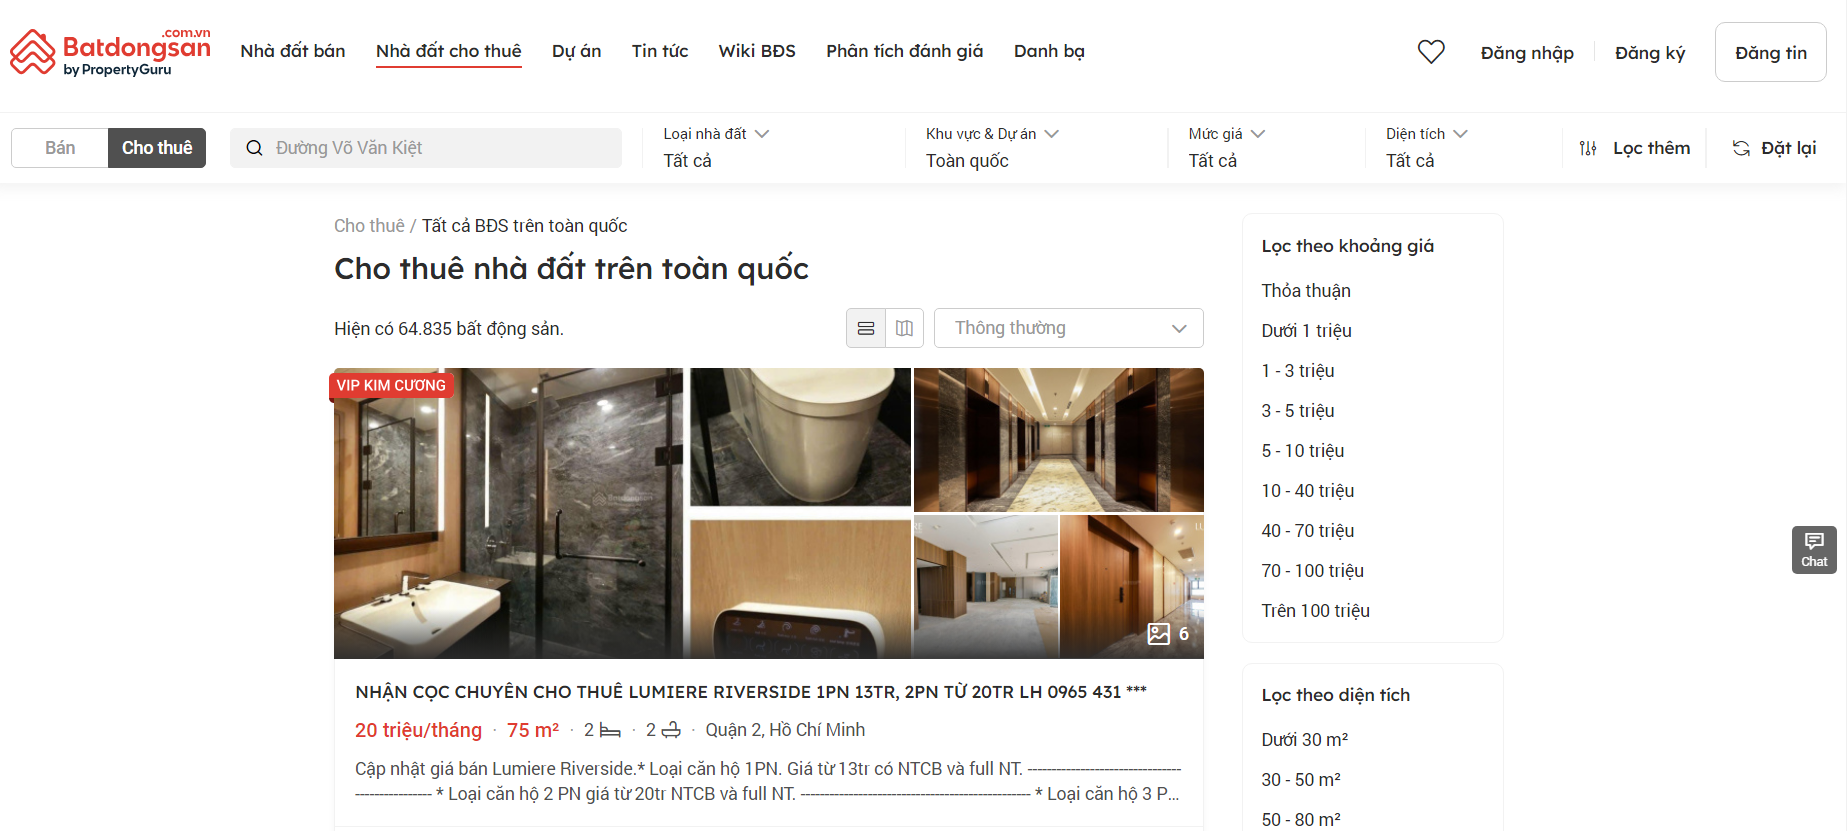
\includegraphics[width=1\textwidth]{Images/RelatedSystems/BatdongsanDesktop.png}
    \caption{Giao diện Batdongsan.com.vn trên website}
\end{figure}
\begin{figure}[H]
    \centering
    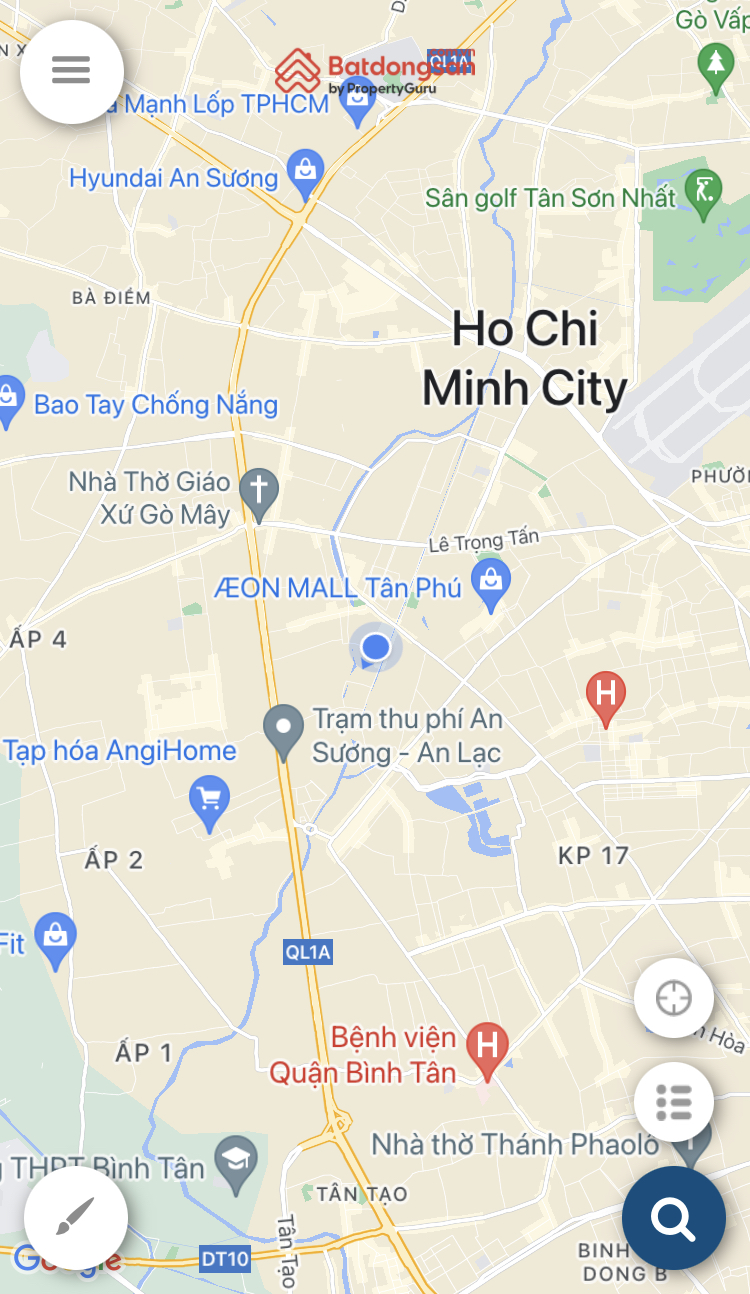
\includegraphics[width=0.5\textwidth]{Images/RelatedSystems/BatdongsanMobile.PNG}
    \caption{Giao diện Batdongsan.com.vn trên thiết bị di động}
\end{figure}
Batdongsan.com.vn là một nền tảng trực tuyến cung cấp thông tin về bất động sản, kết nối người mua, người bán, và những người quan tâm đến thị trường bất động sản. Dưới đây là một số tính năng chính của Batdongsan.com.vn:
\begin{itemize}
    \item \textbf{Tìm kiếm bất động sản}
    \begin{itemize}
    \item \textit{Tìm kiếm theo vị trí:} Người sử dụng có thể tìm kiếm bất động sản theo vị trí cụ thể, chẳng hạn như thành phố, quận, phường.
    \item \textit{Tìm kiếm theo loại bất động sản:} Tính năng này cho phép người dùng lọc kết quả theo loại bất động sản, bao gồm căn hộ, nhà riêng, đất đai, văn phòng, và nhiều loại khác.
    \item \textit{Tìm kiếm theo giá cả:} Người dùng có thể tìm kiếm bất động sản theo khoảng giá cụ thể hoặc khoảng giá ước tính.
    \item \textit{Tìm kiếm nâng cao:} Tính năng này cung cấp các tùy chọn lọc chi tiết hơn, như diện tích, số phòng ngủ, số phòng tắm, và tiện ích xung quanh.
    \end{itemize}
    \item \textbf{Đăng tải}
    \begin{itemize}
        \item \textit{Đăng tin bất động sản:} Người bán có thể đăng thông tin về bất động sản của họ, cung cấp thông tin chi tiết và hình ảnh để thu hút người mua.
        \item \textit{Quản lý tin đăng:} Tính năng này cho phép người bán quản lý và cập nhật thông tin của mình, thêm ảnh mới, chỉnh sửa mô tả, và thực hiện các thay đổi khác.
        \item \textit{Thông báo khi có người quan tâm:} Người bán có thể nhận được thông báo khi có người quan tâm hoặc liên hệ về tin đăng của họ.
    \end{itemize}
    \item \textbf{Thông tin chi tiết}
    \begin{itemize}
        \item \textit{Thông tin chi tiết về bất động sản:} Bất động sản được mô tả chi tiết với các thông tin như diện tích, hướng, tiện ích xung quanh, năm xây dựng,...
        \item \textit{Hình ảnh và video:} Người bán có thể đăng tải hình ảnh và video để người mua có cái nhìn rõ ràng về bất động sản.
        \item \textit{Liên hệ trực tiếp với người bán:} Người mua có thể liên hệ trực tiếp với người bán qua thông tin liên lạc được cung cấp trên trang tin đăng.
    \end{itemize}
    \item \textbf{Tin tức \& Phân tích}
    \begin{itemize}
        \item \textit{Tin tức:} Cung cấp các nội dung tin tức phong phú liên quan đến thị trường bất động sản để giúp người dùng có thể nắm được những thông tin nhanh và mới nhất liên quan đến lĩnh vực bất động sản
        \item \textit{Phân tích:} Những phân tích nhạy bén từ các chuyên gia kinh nghiệm trong lĩnh vực bất động sản, giúp người dùng có thể cân nhắc một cách tối ưu nhất khi đưa ra những quyết định
    \end{itemize}
    \item \textbf{Hỗ trợ}
    \begin{itemize}
        \item \textit{Trung tâm hỗ trợ:} Batdongsan.com.vn cung cấp trung tâm hỗ trợ với thông tin hữu ích và câu hỏi thường gặp để giúp người dùng.
        \item \textit{Hỗ trợ qua điện thoại và email:} Dịch vụ hỗ trợ khách hàng qua điện thoại và email để giải đáp mọi thắc mắc và giúp đỡ người dùng.
    \end{itemize}
\end{itemize}
\subsection{Phân tích SWOT}
\begin{tcbraster}[raster columns=2, boxrule=0mm, arc=0mm]
\begin{tcolorbox}[equal height group=A, size=fbox, colback=swotS!60, colframe=swotS!80!black, title=\textsc{strengths}]
\begin{itemize}
\item Batdongsan.com.vn là một trong những trang web hàng đầu về bất động sản tại Việt Nam, có lượng người dùng lớn.
\item Cung cấp thông tin đa dạng về bất động sản, từ căn hộ, nhà đất đến văn phòng, phục vụ nhu cầu đa dạng của người dùng.
\item Giao diện trực quan, dễ sử dụng, giúp người dùng dễ dàng tìm kiếm và đăng tải tin rao bán.
\item Được đầu tư bởi PropertyGuru, một trong những công ty hàng đầu về dịch vụ bất động sản châu Á, để nâng cao chất lượng dịch vụ và khả năng tiếp cận thị trường.
\end{itemize}
\end{tcolorbox}
\begin{tcolorbox}[equal height group=A, size=fbox, colback=swotW!60, colframe=swotW!80!black, title=\textsc{weaknesses}]
\begin{itemize}
\item Chất lượng thông tin về bất động sản phụ thuộc nhiều vào người đăng tin, có thể gây ra tình trạng thông tin không chính xác hoặc thiếu đầy đủ.
\item Cạnh tranh cao từ các trang web và ứng dụng bất động sản khác, đòi hỏi Batdongsan.com.vn duy trì và nâng cao chất lượng dịch vụ để giữ chân người dùng.
\item Quảng cáo có thể làm ảnh hưởng đến trải nghiệm người dùng trên trang web.
\item Một số vấn đề về pháp lý và thuế có thể phức tạp, đặt ra những thách thức cho hoạt động kinh doanh của Batdongsan.com.vn.
\end{itemize}
\end{tcolorbox}
\begin{tcolorbox}[equal height group=B, size=fbox, colback=swotO!60, colframe=swotO!80!black, title=\textsc{opportunities}]
\begin{itemize}
\item Sự phát triển nhanh chóng của thị trường bất động sản ở Việt Nam, tạo ra cơ hội cho Batdongsan.com.vn mở rộng hoạt động và tăng cường thị phần.
\item Khả năng tích hợp trí tuệ nhân tạo để cải thiện trải nghiệm người dùng và tăng tính tương tác.
\item Nhu cầu về bất động sản thông minh và hiện đại đang tăng, có thể làm tăng cơ hội cho Batdongsan.com.vn cung cấp thông tin về các dự án mới và hiện đại.
\item Hợp tác và đầu tư từ các đối tác lớn có thể giúp Batdongsan.com.vn mở rộng và cập nhật công nghệ.
\end{itemize}
\end{tcolorbox}
\begin{tcolorbox}[equal height group=B, size=fbox, colback=swotT!60, colframe=swotT!80!black, title=\textsc{threats}]
\begin{itemize}
\item Thị trường bất động sản có thể chịu ảnh hưởng lớn từ các yếu tố kinh tế và chính trị, ảnh hưởng đến nhu cầu và giá trị bất động sản.
\item Cạnh tranh cao từ các đối thủ trong và ngoài nước, có khả năng cướp khách hàng và thị phần.
\item Thay đổi trong quy định pháp lý và thuế có thể tác động đến hoạt động kinh doanh của Batdongsan.com.vn.
\item Các vấn đề về an toàn thông tin và bảo mật dữ liệu có thể ảnh hưởng đến niềm tin người dùng và hình ảnh thương hiệu.
\end{itemize}
\end{tcolorbox}
\captionof{table}{Phân tích SWOT cho Batdongsan.com.vn (PropertyGuru)}
\end{tcbraster}
\subsection{Nhận xét}
\hspace*{1cm}Batdongsan.com.vn by PropertyGuru đã đạt được vị thế lớn trong lĩnh vực bất động sản tại Việt Nam, mang lại nhiều lợi ích cho cả người mua và người bán. Nền tảng này cung cấp một nguồn thông tin đa dạng về bất động sản, giúp người mua dễ dàng tìm kiếm và so sánh. Được hỗ trợ bởi PropertyGuru, một doanh nghiệp lớn trong lĩnh vực bất động sản châu Á, đã giúp nâng cao chất lượng dịch vụ và mở rộng khả năng tiếp cận thị trường.\\
\hspace*{1cm}Giao diện trực quan và dễ sử dụng của Batdongsan.com.vn cũng là một điểm mạnh, tạo ra trải nghiệm người dùng tích cực. Việc cung cấp thông tin đầy đủ và chính xác về bất động sản giúp người mua có quyết định đúng đắn khi lựa chọn chỗ ở. Hơn nữa, cơ hội để đầu tư và phát triển trong ngành bất động sản đang ngày càng mở rộng.\\
\hspace*{1cm}Tuy nhiên, để duy trì vị thế của mình, Batdongsan.com.vn cũng phải đối mặt với một số thách thức. Cạnh tranh cao từ các đối thủ trong và ngoài nước đặt ra áp lực để duy trì và nâng cao chất lượng dịch vụ. Ngoài ra, các vấn đề pháp lý và thuế cũng có thể tác động đến hoạt động kinh doanh của họ. Điều này đòi hỏi sự quan tâm và linh hoạt trong quản lý để đối mặt với những thách thức này và tiếp tục phát triển một cách bền vững.
\section{NHÀ TỐT (CHỢ TỐT)}
\subsection{Giới thiệu}
\hspace*{1cm} Nhà Tốt là một nền tảng được ra mắt bởi Chợ Tốt, là nền tảng mua bán sản phẩm và kết nối dịch vụ trực tuyến với 12 triệu người dùng cũng như 55 triệu lượt truy cập hàng tháng, cung cấp những dịch vụ liên quan đến bất động sản. Trang web được ra mắt với định hướng giúp tạo ra một giải pháp thuận tiện và nhanh chóng nhất để người mua và người thuê có thể tìm kiếm được bất động sản phù hợp nhất với nhu cầu của mình. Nơi đây, người sử dụng có thể tìm kiếm và có được những thông tin trực quan, đầy đủ về những loại hình bất động sản đa dạng, phổ biến. Vào tháng 3 năm 2023, đã có 500.000 bất động sản ở khắp các tỉnh thành được đăng tải trên nền tảng Nhà Tốt. \cite{nhatot}\\
\hspace*{1cm} Với giao diện sử dụng thân thiện và tính năng tìm kiếm linh hoạt, Nhà Tốt giúp người dùng dễ dàng tìm kiếm và đăng tin mua bán. Đặc biệt, trang web này tập trung vào việc tạo ra một thị trường trực tuyến đáng tin cậy, nơi mà người dùng có thể gặp gỡ và thực hiện giao dịch an toàn. Từ nhà ở, đất đai đến các sản phẩm và dịch vụ khác, Nhà Tốt mang lại trải nghiệm mua sắm đa dạng. Người dùng có thể dễ dàng tìm thấy những thông tin rao bán hoặc cho thuê một cách nhanh chóng và tiện lợi nhất.\\
\begin{figure}[H]
    \centering
    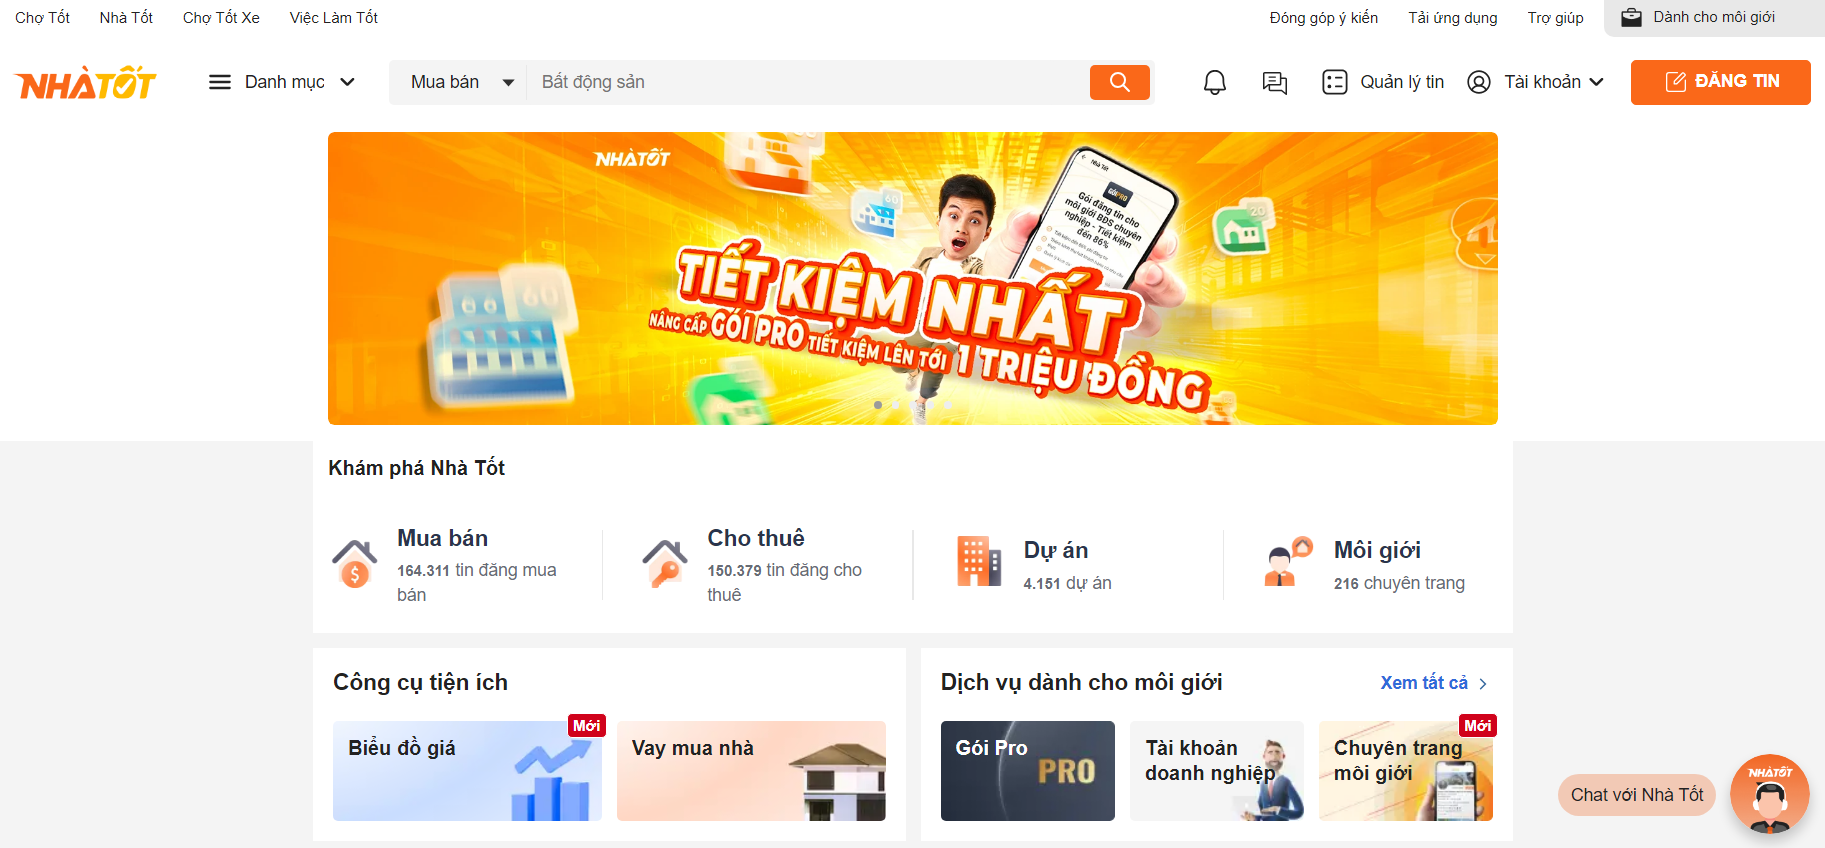
\includegraphics[width=1\textwidth]{Images/RelatedSystems/NhatotDesktop.png}
    \caption{Giao diện Nhà Tốt trên website}
\end{figure}
\begin{figure}[H]
    \centering
    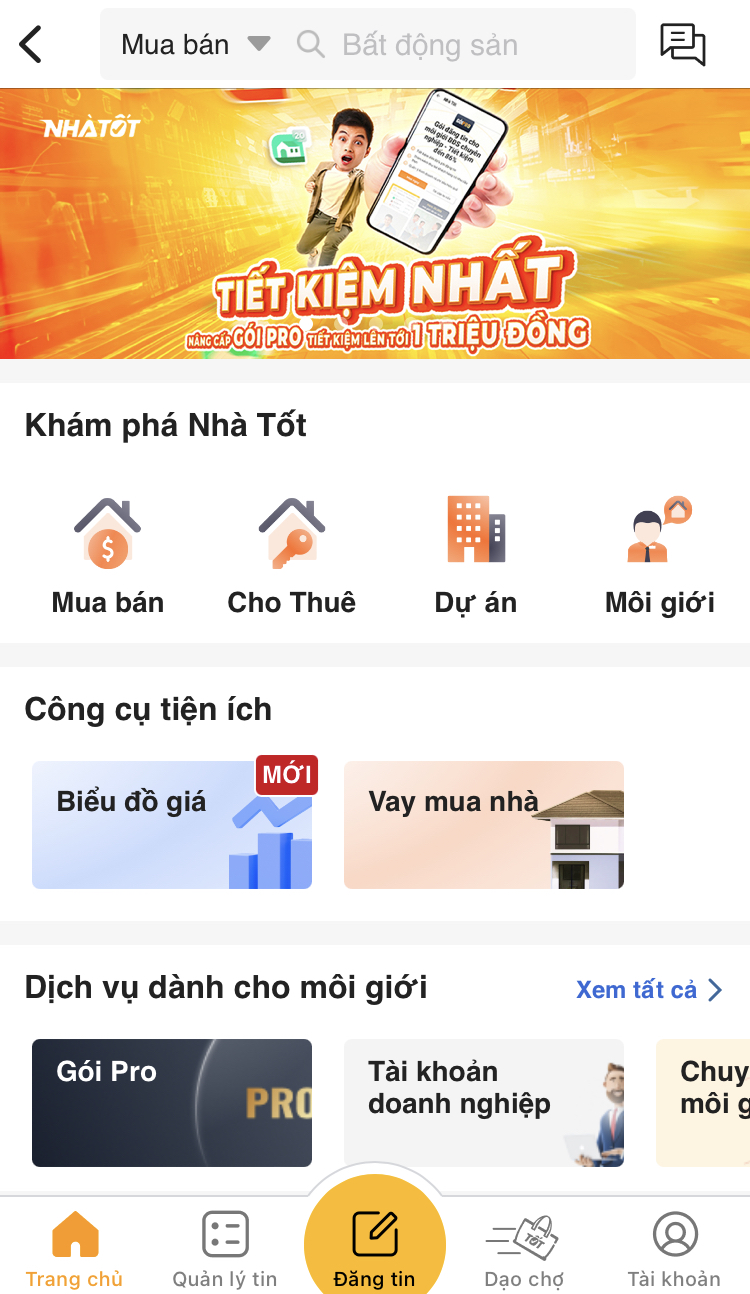
\includegraphics[width=0.5\textwidth]{Images/RelatedSystems/NhatotMobile.PNG}
    \caption{Giao diện Nhà Tốt trên thiết bị di động}
\end{figure}
\subsection{Các tính năng chính}
Nhà Tốt là một nền tảng trực tuyến kết nối người mua, người bán, và những người quan tâm đến thị trường bất động sản. Dưới đây là một số tính năng chính của Nhà Tốt:
\begin{itemize}
    \item \textbf{Tìm kiếm bất động sản}
    \begin{itemize}
        \item \textit{Tìm kiếm theo vị trí:} Người sử dụng có thể tìm kiếm bất động sản theo vị trí cụ thể, chẳng hạn như thành phố, quận, phường
        \item \textit{Phân loại theo danh mục:} Phân loại bất động sản mua bán, cho thuê, tìm kiếm các dự án đang được phát triển
        \item \textit{Bộ lọc nâng cao}: Lọc các kết quả bất động sản tìm được dựa trên khoảng giá, diện tích, số phòng.
    \end{itemize}
    \item \textbf{Đăng tải bất động sản}
    \begin{itemize}
        \item \textit{Đăng tin bất động sản:} Người dùng có thể đăng tải bài đăng về cho thuê hoặc mua bán bất động sản, có thể cung cấp các hình ảnh trực quan về bất động sản và các thông tin chi tiết khác để người dùng dễ tiếp cận
        \item \textit{Quản lý tin đăng:} Người dùng quản lý tin đăng thông qua việc chỉnh sửa bài đăng hoặc có thể gỡ bỏ bài đăng bất động sản.
    \end{itemize}
    \item \textbf{Tương tác giữa người mua và người bán:}
    \begin{itemize}
        \item \textit{Số điện thoại liên hệ:} Người đăng sẽ để lại số điện thoại liên hệ trên bài đăng và khi có nhu cầu, người mua hoặc thuê sẽ gọi đến người đăng thông qua số điện thoại đó.
        \item \textit{Trò chuyện trực tiếp:} Người đăng và người mua hoặc thuê có thể nhắn tin trực tiếp với nhau thông qua ứng dụng.
        \item \textit{Gửi câu hỏi:} Người mua hoặc thuê cũng có thể để lại câu hỏi và đợi người đăng phản hồi lại trong một khoảng thời gian.
    \end{itemize}
    \item \textbf{Trung tâm trợ giúp}:
    \begin{itemize}
        \item \textit{Hướng dẫn:} Nhà Tốt cung cấp các hướng dẫn chi tiết dành cho người mua và người bán trên ứng dụng, họ có thể tiếp cận những hướng dẫn để giúp cho việc trải nghiệm trên ứng dụng được hiệu quả hơn
        \item \textit{Các câu hỏi phổ biến:} Người dùng có thể tìm kiếm nhanh chóng những vấn đề phổ biến thường gặp khi trải nghiệm ứng dụng và giải đáp cho những vấn đề đó.
        \item \textit{Trò chuyện trực tiếp:} Bất cứ lúc nào, người dùng có thể liên lạc trực tiếp với trợ lý ảo của chợ tốt để giải đáp cụ thể những thắc mắc hay những vấn đề có thể gặp phải
    \end{itemize}
\end{itemize}
\subsection{Phân Tích SWOT}
\begin{tcbraster}[raster columns=2, boxrule=0mm, arc=0mm]
\begin{tcolorbox}[equal height group=A, size=fbox, colback=swotS!60, colframe=swotS!80!black, title=\textsc{strengths}]
\begin{itemize}
\item Nhà Tốt là một thương hiệu bất động sản uy tín, được nhiều người biết đến. Thương hiệu này đã được xây dựng trong nhiều năm qua, thông qua các hoạt động quảng bá tích cực, cũng như chất lượng dịch vụ tốt.
\item Nhà Tốt có lượng người truy cập lớn, đa dạng, bao gồm cả người mua, người bán và các nhà đầu tư bất động sản. Điều này cho thấy website của Nhà Tốt đã thu hút được sự quan tâm của nhiều đối tượng khách hàng.
\end{itemize}
\end{tcolorbox}
\begin{tcolorbox}[equal height group=A, size=fbox, colback=swotW!60, colframe=swotW!80!black, title=\textsc{weaknesses}]
\begin{itemize}
\item Nội dung website của Nhà Tốt chưa được cập nhật thường xuyên, khiến cho website trở nên thiếu cập nhật, thiếu hấp dẫn.
\item Trải nghiệm người dùng trên website của Nhà Tốt chưa được tối ưu, khiến cho người dùng gặp khó khăn trong việc tìm kiếm thông tin, sử dụng các tính năng trên website.
\item Nhà Tốt chưa có nhiều tính năng mới, hấp dẫn, đáp ứng nhu cầu của người dùng.
\item Nhà Tốt chưa tận dụng được sức mạnh của các kênh truyền thông xã hội để tiếp cận với nhiều khách hàng hơn.
\end{itemize}
\end{tcolorbox}
\begin{tcolorbox}[equal height group=B, size=fbox, colback=swotO!60, colframe=swotO!80!black, title=\textsc{opportunities}]
\begin{itemize}
\item Thị trường bất động sản Việt Nam đang phát triển mạnh mẽ, tạo ra nhiều cơ hội cho các trang web bất động sản. Nhu cầu tìm kiếm nhà đất của người dân ngày càng tăng, tạo ra nhiều tiềm năng cho các trang web bất động sản.
\item Công nghệ đang phát triển, tạo ra nhiều cơ hội mới cho các trang web bất động sản, như: phát triển các tính năng mới, hấp dẫn, tối ưu trải nghiệm người dùng,...
\item Tăng trưởng của các kênh thương mại điện tử tạo ra cơ hội cho các trang web bất động sản mở rộng hoạt động kinh doanh của mình sang các lĩnh vực khác như: môi giới, tư vấn bất động sản,...
\end{itemize}
\end{tcolorbox}
\begin{tcolorbox}[equal height group=B, size=fbox, colback=swotT!60, colframe=swotT!80!black, title=\textsc{threats}]
\begin{itemize}
\item Sự cạnh tranh ngày càng gay gắt từ các trang web bất động sản khác, khiến cho Nhà Tốt cần phải nỗ lực hơn nữa để giữ vững vị thế của mình.
\item Thị trường bất động sản thay đổi nhanh chóng, khiến cho Nhà Tốt cần phải cập nhật thông tin thường xuyên, để cung cấp cho khách hàng những thông tin chính xác, kịp thời.
\item Luật pháp, quy định liên quan đến bất động sản có thể thay đổi, khiến cho Nhà Tốt cần phải cập nhật những thay đổi này, để đảm bảo tuân thủ đúng quy định.
\end{itemize}
\end{tcolorbox}
\captionof{table}{Phân tích SWOT cho Nhà Tốt}
\end{tcbraster}
\subsection{Nhận xét}
\hspace*{1cm}Nhà Tốt không chỉ là một ứng dụng tìm kiếm bất động sản thông thường, mà còn là nơi kết nối cộng đồng bất động sản, tạo ra một môi trường tương tác động và tích cực. Giao diện trực quan và tiện ích đa dạng của ứng dụng tạo ra một trải nghiệm người dùng linh hoạt và thú vị, đồng thời tạo ra một giải pháp tiện lợi nhanh chóng trong việc giao dịch bất động sản.\\
\hspace*{1cm}Một điểm mạnh lớn của Nhà Tốt là khả năng kết nối người mua và người bán một cách nhanh chóng và thuận lợi. Hệ thống thông tin đầy đủ và chính xác giúp người mua hiểu rõ hơn về các bất động sản, từ đó đưa ra quyết định mua bán chính xác và linh hoạt. Hơn nữa, việc tận dụng công nghệ để cung cấp thông tin thị trường và xu hướng giúp người dùng nắm bắt tốt hơn về cơ hội đầu tư và phát triển. Sự đổi mới không chỉ là về trải nghiệm người dùng mà còn về mô hình kinh doanh. Nhà Tốt có thể tận dụng mạng lưới xã hội để xây dựng uy tín và đánh giá cộng đồng, tạo ra sự minh bạch và tin cậy trong quá trình giao dịch bất động sản.\\
\hspace*{1cm}Tuy nhiên, Nhà Tốt cũng phải đối mặt với những thách thức, như cạnh tranh khốc liệt từ các đối thủ cũng như việc quản lý vấn đề pháp lý và thuế. Điều này đòi hỏi sự tập trung và linh hoạt từ đội ngũ quản lý để đảm bảo bền vững trong hoạt động kinh doanh.Tóm lại, sự xuất hiện của Nhà Tốt không chỉ là một thách thức mà còn là cơ hội để nâng cao chất lượng dịch vụ và đáp ứng nhu cầu đa dạng của thị trường bất động sản ngày càng phát triển tại Việt Nam.
\section{TỔNG KẾT}
\subsection{Điểm tương đồng}
Cả ba giải pháp Airbnb, Batdongsan và Nhà Tốt đều có những điểm chung sau:
\begin{itemize}
    \item \textbf{Cho thuê bất động sản:} Cả ba trang web/ứng dụng đều cung cấp dịch vụ cho thuê bất động sản, bao gồm nhà riêng, căn hộ, đất nền, nhà phố, biệt thự,...
    \item \textbf{Tìm kiếm dựa trên các tiêu chí và bộ lọc:} Người dùng có thể sử dụng từ khóa tìm kiếm kết hợp với bộ lọc để tìm ra bài đăng cho thuê một cách nhanh chóng và phù hợp nhất với nhu cầu
    \item \textbf{Đăng tải và quản lý bài đăng:} Người đăng có thể đăng tải và quản lý thông tin đăng tải một cách nhanh chóng và dễ dàng
    \item \textbf{Trung tâm hỗ trợ:} Người dùng có thể nhanh chóng tiếp cận với những vấn đề phổ biến thông qua chuyên mục hỗ trợ và nhận được giải đáp.
    \item \textbf{Ứng dụng di động:} Người dùng có thể sử dụng ứng dụng trên ứng dụng di động của cả hai nền tảng Android và iOS.
\end{itemize}
\subsection{Điểm khác biệt}
\begin{center}
    \begin{tabular}{|m{4cm}|m{4cm}|m{4cm}|m{4cm}|}
    \hline
    \bf Chức năng, tiêu chí
    & 
    
\includegraphics[width=0.2\textwidth]{Images/RelatedSystems/Airbnb.png}
    &
    
\includegraphics[width=0.2\textwidth]{Images/RelatedSystems/Batdongsan.jpg}
    &
    
\includegraphics[width=0.2\textwidth]{Images/RelatedSystems/NhaTot.png}
    \tabularnewline\hline
    \centering\textit{Loại hình dịch vụ} & Cho thuê ngắn hạn & Mua bán, cho thuê bất động sản & Mua bán, cho thuê bất động sản
    \tabularnewline\hline
    \centering\textit{Đối tượng sử dụng} & Khách du lịch, người công tác & Người có nhu cầu mua bán, thuê bất động sản & Người có nhu cầu mua bán, thuê bất động sản
    \tabularnewline\hline
    \centering\textit{Phạm vi hoạt động} & Toàn cầu & Việt Nam & Việt Nam
    \tabularnewline\hline
    \centering\textit{Đánh giá và bình luận} & Có & Không & Có
    \tabularnewline\hline
    \centering\textit{Tương tác giữa người đăng và người xem} & Để lại câu hỏi cho người đăng tin & Nhắn tin qua Zalo & Nhắn tin qua ứng dụng, để lại câu hỏi
    \tabularnewline\hline
    \centering\textit{Hoạt động du lịch} & Có & Không & Không
    \tabularnewline\hline
    \centering\textit{Quy đổi tiền tệ} & Có & Không & Không
    \tabularnewline\hline
    \centering\textit{Tin tức và Phân tích} & Không & Có & Không
    \tabularnewline\hline
    \centering\textit{Trợ lý ảo} & Không & Không & Có
    \tabularnewline\hline
    \end{tabular}
    \captionof{table}{So sánh sự khác biệt giữa Airbnb, Batdongsan.com.vn và Nhà Tốt}
\end{center}
\chapter{GIẢI PHÁP ĐỀ XUẤT}
\section{MÔ HÌNH TÌM KIẾM HYBRID}
\subsection{Xử lý dữ liệu}
\begin{figure}[H]
    \centering
    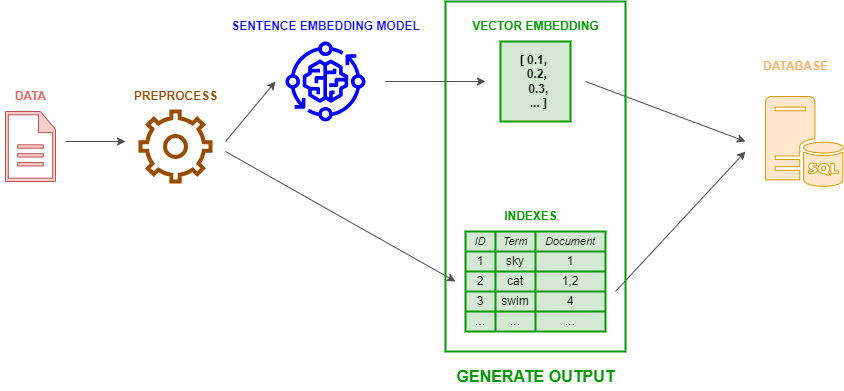
\includegraphics[,width=\textwidth]{Images/HybridSearch/DataProcess.png}
    \caption{Sơ đồ các bước xử lý dữ liệu cho mô hình tìm kiếm Hybrid}
\end{figure}
Quá trình xử lý dữ liệu cho mô hình tìm kiếm bao gồm các bước sau:
\begin{itemize}
    \item Làm sạch dữ liệu:
    \begin{itemize}
        \item Dữ liệu dạng chuỗi (string) được làm sạch để loại bỏ các ký tự đặc biệt, khoảng trắng thừa, và chuẩn hóa văn bản. Quá trình này giúp cải thiện chất lượng và độ chính xác của việc tìm kiếm.
        \item Các bước làm sạch bao gồm: chuyển đổi toàn bộ văn bản về chữ thường, loại bỏ dấu câu, loại bỏ các từ dư thừa hoặc không cần thiết (stop words), và xử lý các lỗi chính tả cơ bản.
    \end{itemize}
    \item Chuyển đổi văn bản thành vector(Embedding):
    \begin{itemize}
        \item Nhóm sử dụng Sentence Transformer để chuyển đổi văn bản đã làm sạch thành các vector số học (embedding). Các vector này biểu thị ý nghĩa ngữ nghĩa của văn bản, giúp hệ thống hiểu được ngữ cảnh và ý định của người dùng.
        \item Quá trình embedding tạo ra các vector có độ chiều cao (high-dimensional vectors), cho phép so sánh và tìm kiếm ngữ nghĩa một cách hiệu quả.
    \end{itemize}
    \item Đánh chỉ mục (Indexing):
    \begin{itemize}
        \item Dữ liệu văn bản sau khi làm sạch cũng được đánh chỉ mục để sử dụng cho việc tìm kiếm toàn văn bản. Việc đánh chỉ mục giúp tăng tốc độ truy vấn, đảm bảo rằng các từ khóa người dùng nhập sẽ được tìm kiếm và so khớp một cách nhanh chóng.
    \end{itemize}
    \item Lưu trữ vào cơ sở dữ liệu:
    \begin{itemize}
        \item Cả vector embedding và chỉ mục của dữ liệu văn bản được lưu trữ trong cơ sở dữ liệu. Điều này giúp hệ thống truy cập và sử dụng thông tin một cách hiệu quả khi thực hiện các truy vấn tìm kiếm.
    \end{itemize}
\end{itemize}
\begin{figure}[H]
    \centering
    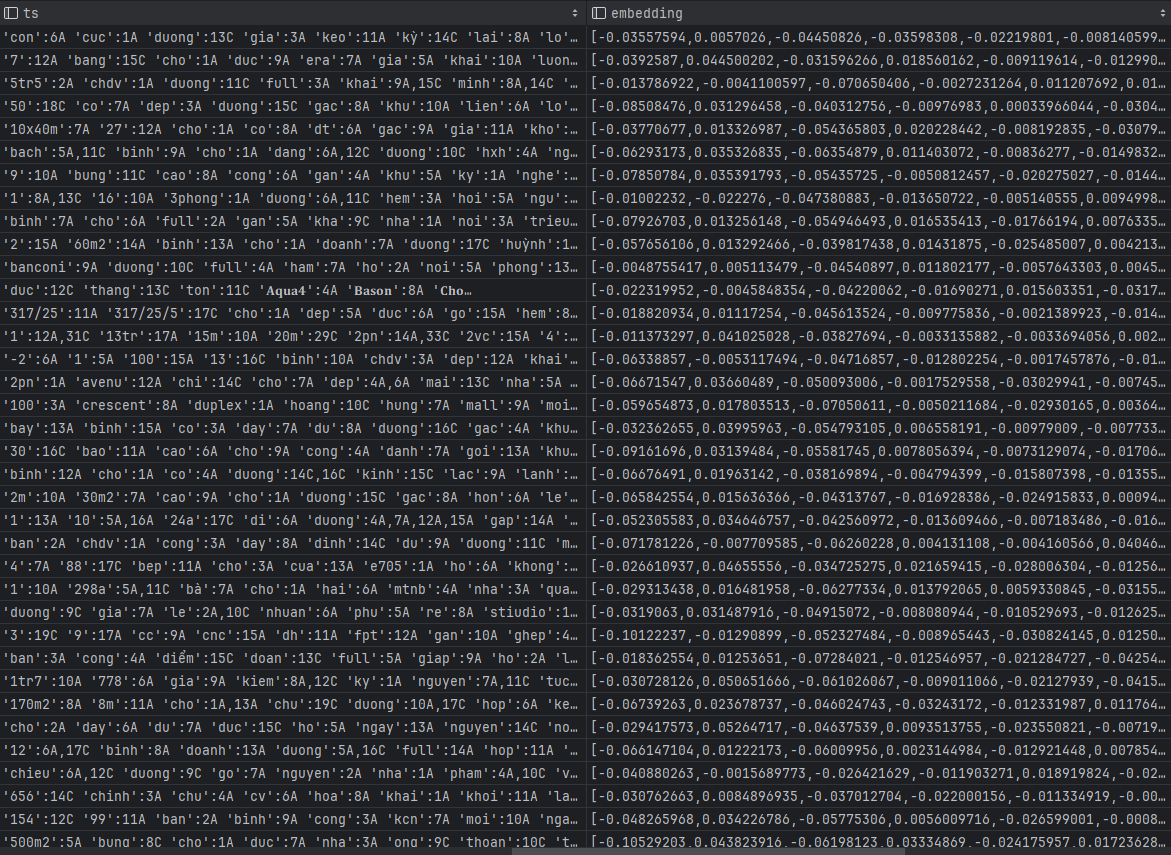
\includegraphics[width=\textwidth]{Images/HybridSearchResult.png}
    \caption{Dữ liệu văn bản sau khi được đánh chỉ mục và chuyển đổi thành dạng vector}
\end{figure}

\subsection{Kiến trúc tìm kiếm với mô hình Hybrid}
Mô hình Hybrid Search kết hợp cả Tìm kiếm toàn văn bản và Tìm kiếm ngữ nghĩa, cùng với cơ chế reranking để tối ưu hóa kết quả tìm kiếm, đảm bảo trải nghiệm tìm kiếm chính xác và hiệu quả cho người dùng. Dưới đây là chi tiết về kiến trúc mô hình:
\begin{figure}[H]
    \centering
    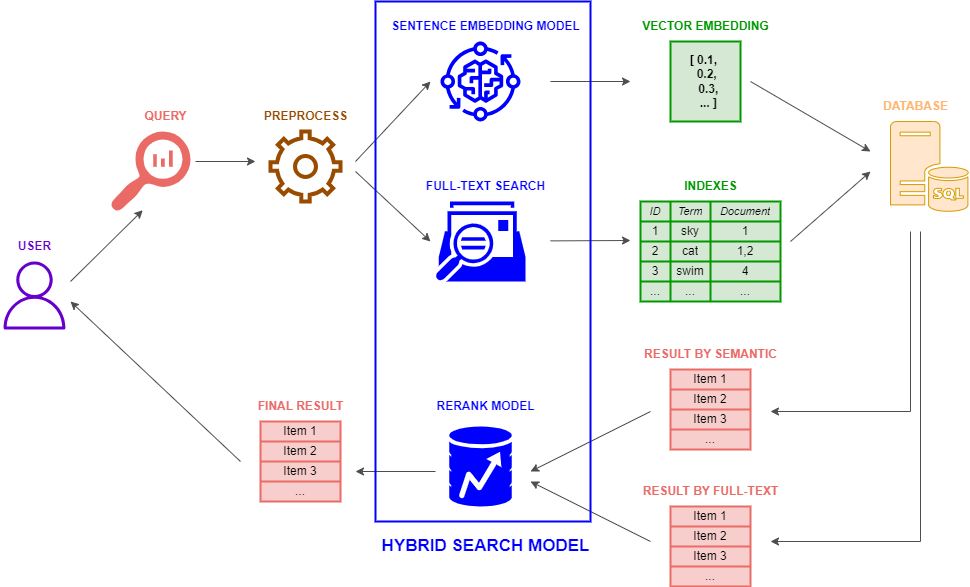
\includegraphics[width=\textwidth]{Images/HybridSearch/SearchArchitecture.png}
    \caption{Sơ đồ kiến trúc của mô hình tìm kiếm Hybrid}
\end{figure}
Mô hình hybrid search kết hợp giữa Tìm kiếm toàn văn bản và Tìm kiếm ngữ nghĩa gồm:
\begin{itemize}
    \item User: Người dùng nhập câu truy vấn (query) vào hệ thống tìm kiếm.
    \item Câu truy vấn từ người dùng được tiếp nhận và chuyển đến bước tiền xử lý.
    \item  Preprocess query: câu truy vấn được làm sạch bằng cách loại bỏ ký tự đặc biệt và chuyển về chữ thường.
    \item Vector embedding: Câu truy vấn đã làm sạch được chuyển đổi thành vector sử dụng Sentence Transformer, giúp biểu diễn ngữ nghĩa của câu truy vấn.
    \item Indexes: Dữ liệu văn bản đã được làm sạch trước đó được đánh chỉ mục. Các chỉ mục này giúp tăng tốc độ truy vấn và tìm kiếm các từ khóa cụ thể trong cơ sở dữ liệu.
    \item Database: Lưu trữ cả dữ liệu gốc, dữ liệu đã đánh chỉ mục toàn văn và các vector embedding. Điều này đảm bảo hệ thống có thể thực hiện cả tìm kiếm toàn văn và tìm kiếm ngữ nghĩa.
    \item Quy trình tìm kiếm:
    \begin{itemize}
        \item Thực hiện tìm kiếm toàn văn trước tiên dựa trên từ khóa trong chỉ mục toàn văn. 
        \item  Nếu kết quả tìm kiếm từ Full Text Search đủ tốt, hệ thống sẽ chuyển sang bước reranking. Nếu không đủ tốt, hệ thống sẽ chuyển sang tìm kiếm ngữ nghĩa.
        \item Tìm kiếm ngữ nghĩa: Sử dụng vector embedding của câu truy vấn để so sánh với các vector của dữ liệu đã lưu trữ và tìm kiếm các kết quả ngữ nghĩa.
    \end{itemize}
    \item Reranking: Kết quả từ cả Tìm kiếm toàn văn và Tìm kiếm ngữ nghĩa được đưa vào mô hình Cross-Encoder để sắp xếp lại. Cross-Encoder sẽ xem xét cặp truy vấn-kết quả và tính điểm độ phù hợp cao hơn, giúp cải thiện độ chính xác của kết quả cuối cùng.
    \item Sau khi được reranking, kết quả cuối cùng sẽ được trả về cho người dùng
\end{itemize}
\definecolor{AppGreen}{HTML}{10b981}
\section{GIỚI THIỆU ỨNG DỤNG TÌM KIẾM NHÀ TRỌ}
\subsection{Tên ứng dụng}
Tên gọi của ứng dụng là \textbf{\color{AppGreen} HOURSENET}, tên gọi trên có ý nghĩa như sau:
\begin{itemize}
    \item \textbf{\textit{HOUSE:}} Đây là từ cơ bản nhất, có nghĩa là \textit{"nhà"}. Nó phản ánh rõ ràng mục đích chính của ứng dụng là tìm kiếm và thuê nhà.
    \item \textbf{\textit{OUR:}} Từ này được hiểu là \textit{"của chúng ta"}. Điều này tạo cảm giác thân thiện và kết nối, như thể ứng dụng này là một công cụ dành cho cộng đồng, giúp mọi người tìm kiếm nhà dễ dàng hơn.
    \item \textbf{\textit{NET:}} Từ này được hiểu là \textit{"mạng lưới"} hoặc \textit{"internet"}. Ý nghĩa của từ này đó là ứng dụng sử dụng mạng lưới thông tin rộng lớn trên \textit{internet} để cung cấp dịch vụ tìm kiếm nhà thuê.
\end{itemize}
\subsection{Logo ứng dụng}
\begin{figure}[h]
    \centering
    
\includegraphics[width=0.5\textwidth]{Images/LogoHoursenet.png}
    \caption{Thiết kế logo của ứng dụng Housernet}
\end{figure}
\hspace*{1cm}
\textit{Logo} của ứng dụng \textit{Hoursenet} được thiết kế với hình ảnh trung tâm là một ngôi nhà, được phóng đại qua kính lúp và bao quanh bởi các kết nối mạng lưới. Đây là một \textit{logo} đơn giản nhưng chứa đựng nhiều ý nghĩa sâu sắc, thể hiện rõ mục tiêu và tầm nhìn của ứng dụng.
\begin{itemize}
    \item \textit{Ngôi nhà:} Hình ảnh ngôi nhà ở trung tâm là biểu tượng trực tiếp của mục đích chính của ứng dụng – giúp người dùng tìm kiếm và thuê nhà. Ngôi nhà đại diện cho sự ổn định, an cư và cũng là điều mà người dùng đang tìm kiếm thông qua \textit{Hoursenet}.
    \item \textit{Kính lúp:} Kính lúp tượng trưng cho việc tìm kiếm và khám phá. Điều này thể hiện chức năng chính của ứng dụng là giúp người dùng dễ dàng tìm kiếm các ngôi nhà phù hợp với nhu cầu của họ. Nó nhấn mạnh tính năng thông minh và khả năng tìm kiếm chi tiết của ứng dụng.
    \item \textit{Mạng lưới kết nối:} Các vòng tròn xung quanh ngôi nhà được kết nối bởi các đường nét tượng trưng cho mạng lưới thông tin rộng lớn. Điều này ám chỉ việc ứng dụng sử dụng công nghệ và dữ liệu để kết nối người dùng với các lựa chọn nhà thuê đa dạng và phong phú. Nó cũng thể hiện tính cộng đồng và khả năng liên kết mạnh mẽ của \textit{Hoursenet}.
    \item \textit{Màu xanh lá cây:} Màu xanh lá cây thường gợi liên tưởng đến sự tươi mới, an lành và phát triển bền vững. Việc sử dụng màu xanh làm nền chính cho logo thể hiện cam kết của ứng dụng trong việc mang lại trải nghiệm tốt nhất, đáng tin cậy và thân thiện với người dùng.
\end{itemize}
\subsection{Mô tả ứng dụng}
\hspace*{1cm}
Ứng dụng \textit{Hoursenet} là một giải pháp tìm kiếm nhà cho thuê thông minh, được thiết kế để đáp ứng mọi nhu cầu của người dùng trong việc tìm kiếm và thuê nhà. Với giao diện thân thiện và dễ sử dụng, \textit{Hoursenet} mang đến trải nghiệm tìm kiếm nhà ở hoàn hảo thông qua nhiều tính năng hiện đại và tiện ích.\\
\hspace*{1cm}
Một trong những tính năng nổi bật của \textit{Hoursenet} là khả năng tìm kiếm nhà cho thuê bằng văn bản sử dụng ngôn ngữ tự nhiên. Người dùng chỉ cần nhập các yêu cầu của mình và ứng dụng sẽ hiển thị các kết quả phù hợp một cách nhanh chóng và chính xác.\\
\hspace*{1cm}
Ngoài ra, ứng dụng còn hỗ trợ tính năng bình luận và đánh giá, cho phép người dùng chia sẻ ý kiến và kinh nghiệm của mình về các căn nhà đã thuê. Điều này giúp tạo ra một cộng đồng người dùng tin cậy, nơi mọi người có thể tham khảo những đánh giá chân thực trước khi đưa ra quyết định thuê nhà.\\
\hspace*{1cm}
\textit{Hoursenet} cũng tích hợp công cụ tìm kiếm bằng bộ lọc, giúp người dùng dễ dàng lọc kết quả theo các tiêu chí như giá cả, diện tích, vị trí và nhiều yếu tố khác. Tính năng này giúp tiết kiệm thời gian và công sức cho người dùng trong quá trình tìm kiếm.\\
\hspace*{1cm}
Ứng dụng đã được phát hành trên nền tảng \textit{Android}, mang lại sự tiện lợi cho người dùng có thể truy cập và sử dụng mọi lúc, mọi nơi. Đặc biệt, \textit{Hoursenet} không chỉ hỗ trợ người thuê nhà mà còn cung cấp tính năng đăng tải nhà cho thuê dành cho các chủ nhà. Chủ nhà có thể dễ dàng tạo và quản lý danh sách các căn nhà cho thuê, giúp kết nối nhanh chóng với người có nhu cầu thuê.\\
\hspace*{1cm}
Với \textit{Hoursenet}, việc tìm kiếm và thuê nhà trở nên đơn giản và hiệu quả hơn bao giờ hết. Ứng dụng không chỉ là công cụ tìm kiếm mà còn là cầu nối tin cậy giữa người thuê và chủ nhà, mang đến trải nghiệm thuê nhà tốt nhất cho mọi người.
\section{XÂY DỰNG YÊU CẦU HỆ THỐNG}
\subsection{Yêu cầu chức năng}
Ứng dụng cung cấp thông tin về phòng trọ cũng như quản lý phòng trọ bao gồm các chức năng chính như sau: 
\begin{itemize}
    \item Ứng dụng phải cung cấp các thông tin cơ bản về nhà trọ để tất cả người dùng có thể tham khảo như tiện ích, địa chỉ, giá thuê,...
    \item Ứng dụng được dùng như một công cụ giúp người cho thuê có thể quảng bá nhà trọ của mình với cộng đồng sử dụng ứng dụng bằng cách đăng tải các thông tin chi tiết lên trang chủ ứng dụng
    \item Giao diện cần được thiết kế thân thiện và dễ sử dụng, nhằm giảm thiểu thời gian mà người dùng cần để học cách sử dụng. Ngoài ra, nó cần được tối ưu hóa để đáp ứng nhanh chóng nhu cầu và mong muốn của người dùng khi tìm kiếm nhà trọ
\end{itemize}
\subsection{Stakeholder}
Ứng dụng được phát triển để phục vụ các nhóm đối tượng sau:
\begin{itemize}
    \item Người dùng
    \begin{itemize}
        \item Là những người sử dụng ứng dụng với một trong hai vai trò : người thuê trọ hoặc chủ trọ
        \item Nhóm người dùng này có các chức năng cơ bản thường xuyên xuất hiện trên các ứng dụng như :
        \begin{itemize}
            \item[+] Tìm kiếm nhà trọ dưa trên các từ khóa hoặc bộ lọc các thông tin các từ khóa như: thành phố, quận, diện tích, giá thuê, tiện ích,...
            \item[+] Đăng ký và Đăng nhập
            \item[+] Chỉnh sửa thông tin tài khoản như tên , hình ảnh đại diện
            \item[+] Đặt lại mật khẩu trong trường hợp quên mật khẩu
        \end{itemize}
        \item Với vai trò là Người thuê trọ:
        \begin{itemize}
            \item[+] Đây là những cá nhân dùng ứng dụng để tìm kiếm thông tin nhà trọ phù hợp với mong muốn , nhu cầu của bản thân
            \item[+] Ngoài các chức năng cơ bản của người dùng, người thuê còn được cung cấp thêm các chức năng khác như:
            \begin{itemize}
                \item Được gợi ý nhà trọ dựa trên các từ khóa mà người dùng nhập khi tìm kiếm
                \item Đánh giá và viết phản hồi về nhà trọ mà họ đã hoặc đang sử dụng
            \end{itemize}
        \end{itemize}
        \item Với vai trò là Chủ trọ :
        \begin{itemize}
            \item[+] Là người cho thuê các nhà trọ thông qua các bài đăng trên ứng dụng
            \item[+] Bên cạnh các chức năng của người dùng, họ còn có thêm các tính năng riêng biệt như : 
             \begin{itemize}
                \item Đăng tải thông tin nhà trọ dựa theo mẫu có sẵn để điền các trường thông tin mà bài đăng yêu cầu
                \item Chỉnh sửa thông tin nhà trọ như thêm hình ảnh, thay đổi địa chỉ, cập nhật danh sách tiện ích, giá thuê trọ
            \end{itemize}
        \end{itemize}
    \end{itemize}
\end{itemize}
\subsection{Yêu cầu phi chức năng}
\begin{itemize}
    \item Hệ thống có thể đáp ứng tối đa 5000 users cùng lúc.
    \item Database có thể tiếp nhận dữ liệu liên tục từ đồng thời tối đa 100 users.
    \item Hỗ trợ 2 hệ điều hành là Android và iOS.
    \item Ứng dụng hỗ trợ 2 ngôn ngữ Tiếng Anh và Tiếng Việt.
    \item Hệ thống sẽ phản hồi lại cho người dùng trong vòng 1s.
\end{itemize}


\section{SƠ ĐỒ VÀ ĐẶC TẢ USE-CASE}
\input{Section/4. Propose Solution/Use-case/1. Auth}
\input{Section/4. Propose Solution/Use-case/2. Account}
\input{Section/4. Propose Solution/Use-case/3. User}
\input{Section/4. Propose Solution/Use-case/4. GetListing}
\input{Section/4. Propose Solution/Use-case/5. ManageListing}
\input{Section/4. Propose Solution/Use-case/6. Comment}
\input{Section/4. Propose Solution/Use-case/7. Reply}
\newpage
\section{CƠ SỞ DỮ LIỆU}
\subsection{Mô hình thực thể liên kết mở rộng (EERD)}
\begin{figure}[H]
    \centering
    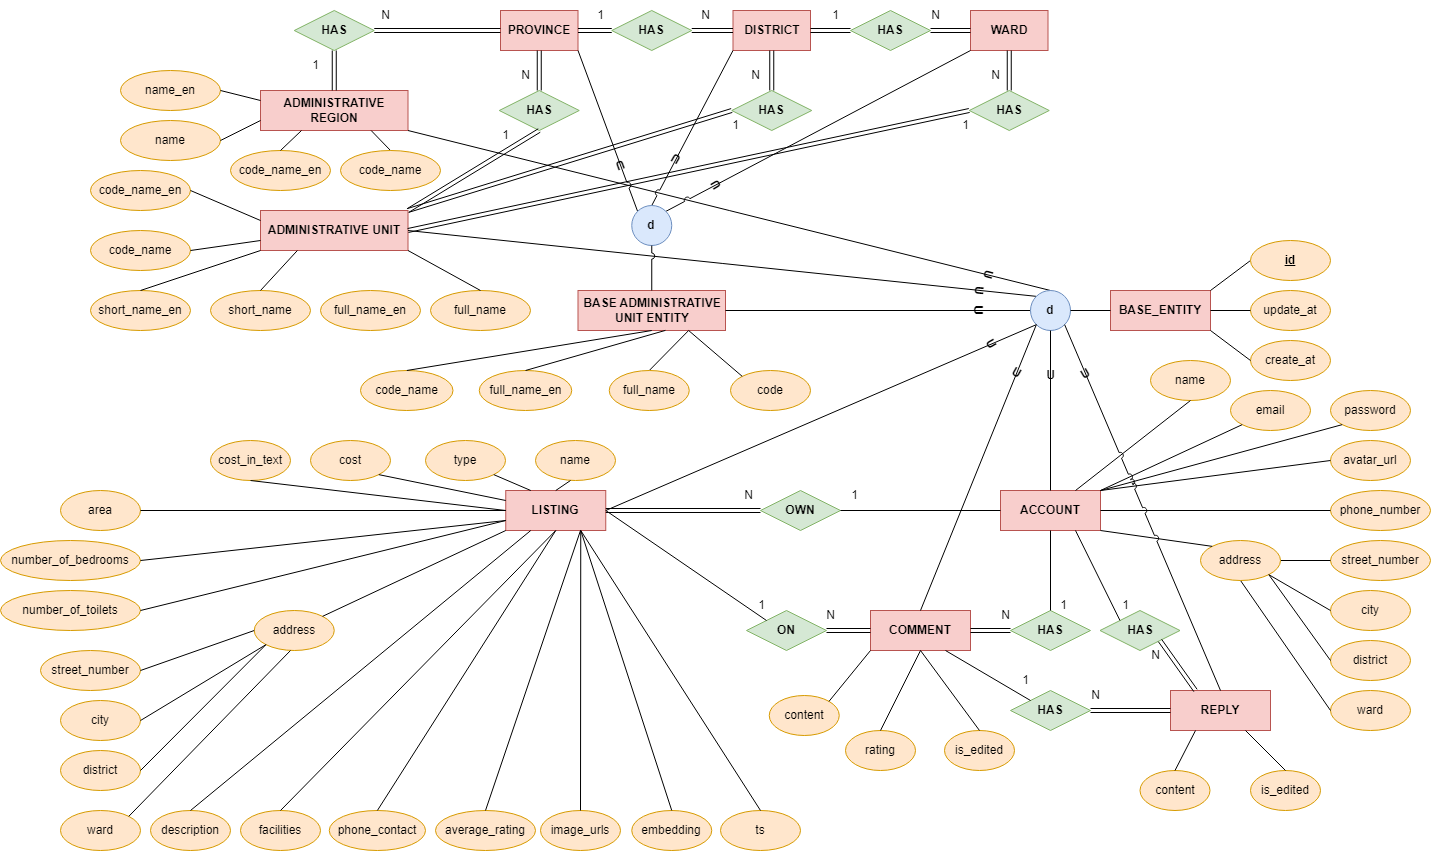
\includegraphics[angle=270,width=0.7\textwidth]{Images/Database/ERD.png}
    \caption{Thiết kế ERD cho cơ sở dữ liệu}
\end{figure}
\subsection{Mô tả thiết kế}
\subsubsection{Các kiểu thực thể}
Trong mô hình EERD trên có 10 thực thể được mô tả như sau:
\begin{itemize}
    \item \textbf{BASE\_ENTITY}: Đây là kiểu thực thể tổng quát để lưu trữ các thuộc tính cần phải được lưu trữ trong các kiểu thực thể còn lại. Các thuộc tính được lưu trữ của kiểu thực thể này bao gồm:
    \begin{itemize}
        \item \underline{\textit{\bf id}}: Thuộc tính khóa dùng để phân biệt các thực thể với nhau trong một kiểu thực thể nhất định.
        \item \textit{create\_at}: Thuộc tính để lưu trữ thời điểm ban đầu mà thực thể dược khởi tạo.
        \item \textit{updated\_at}: Thuộc tính dùng để ghi nhận thời điểm mà thực thể có sự thay đổi ở các thuộc tính.
    \end{itemize}
    \item \textbf{BASE\_ADMINISTRATIVE\_UNIT\_ENTITY}: Đây là kiểu thực thể dùng để lưu trữ các thuộc tính sử dụng chung cho các thực thể \textit{PROVINCE}, \textit{DISTRICT} VÀ \textit{WARD}. Thực thể này có sự kế thừa các thuộc tính từ thực thể \textit{BASE\_ENTITY}. Các thuộc tính được lưu trữ của kiểu thực thể này bao gồm:
    \begin{itemize}
        \item \textit{code}: Mỗi một đơn vị hành chính sẽ có một mã định dang duy nhất được quy định bởi chính phủ Việt Nam
        \item \textit{full\_name}: Tên đầy đủ của đơn vị hành chính bằng tiếng Việt
        \item \textit{full\_name\_en}: Tên đầy đủ của đơn vị hành chính bằng tiếng Anh
        \item \textit{code\_name}: Tên chuẩn hóa của đơn vị hành chính
    \end{itemize}
    \item \textbf{ADMINISTRATIVE\_UNIT}: Đây là kiểu thực thể dùng để lưu trữ các loại cấp bậc của phân cấp đơn vị hành chính trên lãnh thổ Việt Nam. Thực thể này có sự kế thừa các thuộc tính từ thực thể \textit{BASE\_ENTITY}. Các thuộc tính được lưu trữ của kiểu thực thể này bao gồm:
    \begin{itemize}
        \item \textit{full\_name}: Tên đầy đủ của loại cấp bậc đơn vị hành chính bằng tiếng Việt
        \item \textit{full\_name\_en}: Tên đầy đủ của loại cấp bậc của đơn vị hành chính bằng tiếng Anh
        \item \textit{short\_name}: Tên ngắn gọn của loại cấp bậc đơn vị hành chính bằng tiếng Việt
        \item \textit{short\_name\_en}: Tên ngắn của loại cấp bậc của đơn vị hành chính bằng tiếng Anh
        \item \textit{code\_name}: Tên chuẩn hóa của loại cấp bậc đơn vị hành chính bằng tiếng Việt
        \item \textit{code\_name\_en}: Tên chuẩn hóa của loại cấp bậc đơn vị hành chính bằng tiếng Anh
    \end{itemize}
    \item \textbf{ADMINISTRATIVE\_REGION}: Đây là kiểu thực thể dùng để lưu trữ các vùng kinh tế - xã hội trên lãnh thổ Việt Nam. Thực thể này có sự kế thừa các thuộc tính từ thực thể \textit{BASE\_ENTITY}. Các thuộc tính được lưu trữ của kiểu thực thể này bao gồm:
    \begin{itemize}
        \item \textit{name}: Tên đầy đủ của vùng kinh tế - xã hội bằng tiếng Việt
        \item \textit{name\_en}: Tên đầy đủ của vùng kinh tế - xã hội bằng tiếng Anh
        \item \textit{code\_name}: Tên chuẩn hóa của vùng kinh tế - xã hội bằng tiếng Việt
        \item \textit{code\_name\_en}: Tên chuẩn hóa của vùng kinh tế - xã hội bằng tiếng Anh
    \end{itemize}
    \item \textbf{PROVINCE}: Đây là kiểu thực thể dùng để lưu trữ toàn bộ các tỉnh / thành phố trên lãnh thổ Việt Nam. Thực thể này có sự kế thừa các thuộc tính từ các thực thể \textit{BASE\_ENTITY} và \textit{BASE\_ADMINISTRATIVE\_UNIT\_ENTITY}.
    \item \textbf{DISTRICT}: Đây là kiểu thực thể dùng để lưu trữ toàn bộ các quận / huyện và các đơn vị hành chính cấp tương đương trên lãnh thổ Việt Nam. Thực thể này có sự kế thừa các thuộc tính từ các thực thể \textit{BASE\_ENTITY} và \textit{BASE\_ADMINISTRATIVE\_UNIT\_ENTITY}.
    \item \textbf{ward}: Đây là kiểu thực thể dùng để lưu trữ toàn bộ các phường / xã và các đơn vị hành chính cấp tương đương trên lãnh thổ Việt Nam. Thực thể này có sự kế thừa các thuộc tính từ các thực thể \textit{BASE\_ENTITY} và \textit{BASE\_ADMINISTRATIVE\_UNIT\_ENTITY}.
    \item \textbf{ACCOUNT}: Đây là kiểu thực thể dùng để lưu thông tin người dùng sử dụng ứng dụng, người dùng này có thể là người chủ trọ đăng bài thuê trọ và cũng có thể là người có nhu cầu sử dụng ứng dụng để thuê trọ. Thực thể này có sự kế thừa các thuộc tính từ thực thể \textit{BASE\_ENTITY}. Các thuộc tính được lưu trữ của kiểu thực thể này bao gồm:
    \begin{itemize}
        \item \textit{name}: Là tên của người dùng, bao gồm cả họ và tên.
        \item \textit{email}: Là địa chỉ email mà người dùng sử dụng để đăng ký tài khoản cho ứng dụng.
        \item \textit{password}: Là mật khẩu mà người dùng khởi tạo khi đăng ký tài khoản ứng dụng. Trong cơ sở dữ liệu, mật khẩu của người dùng sẽ được băm một chiều nên chỉ có người dùng mới có thể biết được thông tin của mật khẩu.
        \item \textit{phone\_number}: Là số điện thoại mà người dùng có thể ghi nhận đăng ký khi khởi tạo tài khoản, số điện thoại này có thể được dùng để công khai khi người dùng đăng bài viết cho thuê nhà trọ.
        \item \textit{avatar\_url}: Là đường dẫn ứng với hình ảnh đại diện của người dùng, file hình ảnh sẽ được lưu trữ trên dịch vụ lưu trữ đám mây, dịch vụ này sẽ trả về đường dẫn ứng với file hình ảnh đó để lưu trữ trong cơ sở dữ liệu.
        \item \textit{address}: Là địa chỉ sinh sống của người dùng ở thời điểm hiện tại, người dùng có thể tùy ý cung cấp thông tin về địa chỉ cho ứng dụng hoặc không. Thuộc tính \textit{address} bao gồm sự kết hợp của 4 thuộc tính theo phân cấp đơn vị hành chính của Việt Nam như sau:
        \begin{itemize}
            \item \textit{city}: Là tỉnh / thành phố của địa chỉ người dùng
            \item \textit{district}: Là quận / huyện hoặc đơn vị hành chính cấp tương đương của địa chỉ người dùng
            \item \textit{ward}: Là phường / xã hoặc đơn vị hành chính cấp tương đương của địa chỉ người dùng
            \item \textit{street\_number}: Bao gồm số nhà và tên đường / hẻm của địa chỉ người dùng
        \end{itemize}
    \end{itemize}
    \item \textbf{LISTING}: Là kiểu thực thể để lưu trữ thông tin bài đăng tải nhà thuê, thực thể này bao gồm các thuộc tính lưu trữ những thông tin liên quan đến một nhà trọ mà người sử dụng ứng dụng quan tâm khi tìm kiếm, đồng thời cũng lưu trữ các thuộc tính riêng để thực hiện triển khai tìm kiếm trên mô hình Hybrid. Thực thể này có sự kế thừa các thuộc tính từ thực thể \textit{BASE\_ENTITY}. Các thuộc tính được lưu trữ của kiểu thực thể này bao gồm:
    \begin{itemize}
        \item \textit{name}: Tiêu đề của của bài đăng tải nhà thuê.
        \item \textit{type}: Là loại hình cho thuê nhà, cơ sở dữ liệu cho phép người đăng tải được chọn một trong ba loại hình cho thuê bao gồm: \textit{Phòng trọ}, \textit{Căn hộ} hoặc \textit{Nhà đất}.
        \item \textit{cost}: Giá cho thuê nhà theo tháng
        \item \textit{cost\_in\_text}: Giá cho thuê nhà theo tháng được phiên âm thành tiếng Việt. Thuộc tính này nhằm mục đích biểu thị ngữ nghĩa của giá cho thuê nhà trọ để có thể sử dụng tốt trong mô hình tìm kiếm Hybrid.
        \item \textit{area}: Thông tin về diện tích của nhà thuê.
        \item \textit{number\_of\_bedrooms}: Số lượng phòng ngủ.
        \item \textit{number\_of\_toilets}: Số lượng nhà vệ sinh.
        \item \textit{cost}: Giá cho thuê theo tháng.
        \item \textit{cost\_in\_text}: Giá cho thuê theo tháng được phiên âm thành tiếng Việt. Thuộc tính này được lưu trữ nhằm mục đích chuyển đổi từ số sang ngữ nghĩa để sử dụng trong mô hình tìm kiếm hybrid.
        \item \textit{address}: Là địa chỉ của nhà trọ. Tương tự như kiểu thực thể \textbf{ACCOUNT}, thuộc tính \textit{address} bao gồm sự kết hợp của 4 thuộc tính theo phân cấp đơn vị hành chính của Việt Nam như sau:
        \begin{itemize}
            \item \textit{city}: Là tỉnh / thành phố của địa chỉ nhà thuê.
            \item \textit{district}: Là quận / huyện hoặc đơn vị hành chính cấp tương đương của nhà thuê
            \item \textit{ward}: Là phường / xã hoặc đơn vị hành chính cấp tương đương của nhà thuê
            \item \textit{street\_number}: Bao gồm số nhà và tên đường / hẻm ứng với địa chỉ của nhà thuê
        \end{itemize}
        \item \textit{description}: Mô tả ngắn về bài đăng cho thuê nhà.
        \item \textit{facilities}: Các tiện ích của nhà trọ cho thuê, bao gồm danh sách các tiện ích đã được quy ước sẵn trong ứng dụng như: \textit{Tivi}, \textit{Camera giám sát}, \textit{Cảm biến thông minh}, \textit{Máy giặt}, \textit{Tủ lạnh}, \textit{Điều hòa}.
        \item \textit{phone\_contact}: Số điện thoại liên hệ để người sử dụng có thể tiếp cận được với chủ bài đăng.
        \item \textit{average\_rating}: Điểm trung bình của nhà thuê được tính toán dựa trên tất cả các bình luận và đánh giá do những người khác cung cấp cho bài đăng.
        \item \textit{image\_urls}: Lưu trữ các đường dẫn của hình ảnh về nhà thuê để hiển thị khi người dùng xem chi tiết về thông tin bài đăng tải.
        \item \textit{ts}: Thuộc tính dùng để lưu trữ các chỉ mục \textit{indexes} của tất cả các từ ngữ trong bài đăng tải nhà thuê. Thuộc tính này lưu trữ nhằm dùng để phục vụ cho \textit{full-text search}.
        \item \textit{embedding}: Thuộc tính dùng để lưu trữ thông tin ngữ nghĩa về bài đăng nhà thuê dưới dạng \textit{vector}, được sinh ra bởi mô hình \textit{vector embedding}, Thuộc tính này lưu trữ nhằm dùng để phục vụ cho \textit{semantic search}
    \end{itemize}
    \item \textbf{COMMENT}: Kiểu thực thể lưu trữ các bình luận của người dùng đối với một bài đăng tải nhà thuê nhất định. Thực thể này có sự kế thừa các thuộc tính từ thực thể \textit{BASE\_ENTITY}. Các thuộc tính được lưu trữ của kiểu thực thể này bao gồm:
    \begin{itemize}
        \item \textit{content}: Nội dung của bình luận.
        \item \textit{rating}: Điểm đánh giá của người dùng từ 1 đến 5 sao.
        \item \textit{is\_edited}: Biểu thị cho việc người dùng đã chỉnh sửa bình luận hay không.
    \end{itemize}
    \item \textbf{REPLY}: Kiểu thực thể lưu trữ các phản hồi của người dùng cho một bình luận nhất định. Thực thể này có sự kế thừa các thuộc tính từ thực thể \textit{BASE\_ENTITY}. Các thuộc tính được lưu trữ của kiểu thực thể này bao gồm:
    \begin{itemize}
        \item \textit{content}: Nội dung của phản hồi bình luận.
        \item \textit{is\_edited}: Biểu thị cho việc người dùng đã chỉnh sửa phản hồi hay không.
    \end{itemize}
\end{itemize}
\subsubsection{Các mối liên kết}
Các thực thể trong mô hình EERD tồn tại các mối liên kết sau:
\begin{itemize}
    \item ADMINISTRATIVE\_UNIT \textbf{HAS} PROVINCE: Đây là mối liên kết \textit{one - to - many} để biểu thị cho việc một đơn vị hành chính (ở đây là tỉnh, thành phố) phải liên kết với tất cả các tỉnh / thành phố trực thuộc trung ương trên lãnh thổ Việt Nam. Mối liên kết trên có ý nghĩa là tỉnh / thành phố trực thuộc trung ương trong đơn vị phân cấp hành chính phải có sự liên kết đối với tất cả các tỉnh / thành phố trực thuộc trung ương của Việt Nam, và ngược lại, tất cả các tỉnh / thành phố trực thuộc trung ương đều phải được phân loại vào đơn vị hành chính là tỉnh / thành phố trực thuộc trung ương.
    \item ADMINISTRATIVE\_UNIT \textbf{HAS} DISTRICT: Đây là mối liên kết \textit{one - to - many} để biểu thị cho việc một đơn vị hành chính (ở đây là quận / huyện hoặc đơn vị hành chính cấp tương đương) phải liên kết với tất cả các quận / huyện hoặc đơn vị hành chính cấp tương đương trên lãnh thổ Việt Nam. Mối liên kết trên có ý nghĩa là quận / huyện hoặc đơn vị hành chính cấp tương đương trong đơn vị phân cấp hành chính phải có sự liên kết đối với tất cả các quận / huyện hoặc đơn vị hành chính cấp tương đương của Việt Nam, và ngược lại, tất cả các quận / huyện hoặc đơn vị hành chính cấp tương đương đều phải được phân loại vào đơn vị hành chính là quận / huyện hoặc đơn vị hành chính cấp tương đương.
    \item ADMINISTRATIVE\_UNIT \textbf{HAS} WARD: Đây là mối liên kết \textit{one - to - many} để biểu thị cho việc một đơn vị hành chính (ở đây là phường / xã hoặc đơn vị hành chính cấp tương đương) phải liên kết với tất cả các phường / xã hoặc đơn vị hành chính cấp tương đương trên lãnh thổ Việt Nam. Mối liên kết trên có ý nghĩa là phường / xã hoặc đơn vị hành chính cấp tương đương trong đơn vị phân cấp hành chính phải có sự liên kết đối với tất cả các phường / xã hoặc đơn vị hành chính cấp tương đương của Việt Nam, và ngược lại, tất cả các phường / xã hoặc đơn vị hành chính cấp tương đương đều phải được phân loại vào đơn vị hành chính là phường / xã hoặc đơn vị hành chính cấp tương đương.
    \item ADMINISTRATIVE\_REGION \textbf{HAS} PROVINCE: Đây là mối liên kết \textit{one - to - many} để biểu thị cho việc một vùng kinh tế - xã hội phải liên kết với tất cả các tỉnh / thành phố trên phạm vi của vùng kinh tế - xã hội đó. Mối liên kết trên có ý nghĩa là mỗi vùng kinh tế - xã hội phải có nhiều tỉnh / thành phố trực thuộc trung ương, và ngược lại, tất cả các tỉnh / thành phố trực thuộc trung ương trên lãnh thổ Việt Nam đều phải được thuộc về một vùng kinh tế - xã hội nhất định.
    \item PROVINCE \textbf{HAS} DISTRICT: Đây là mối liên kết \textit{one - to - many} để biểu thị cho việc một tỉnh / thành phố trực thuộc trung ương phải liên kết với nhiều quận / huyện hoặc đơn vị hành chính cấp tương đương trên phạm vi của tỉnh / thành phố đó. Mối liên kết trên có ý nghĩa là tỉnh / thành phố phải có nhiều quận / huyện hoặc đơn vị hành chính cấp tương đương, và ngược lại, tất cả các quận / huyện hoặc đơn vị hành chính cấp tương đương đều phải thuộc về một tỉnh / thành phố nhất định.
    \item DISTRICT \textbf{HAS} WARD: Đây là mối liên kết \textit{one - to - many} để biểu thị cho việc một quận / huyện hoặc đơn vị hành chính cấp tương đương phải liên kết với nhiều phường / xã hoặc đơn vị hành chính cấp tương đương trên phạm vi của quận / huyện đó. Mối liên kết trên có ý nghĩa là quận / huyện hoặc đơn vị hành chính cấp tương đương phải có nhiều phường / xã hoặc đơn vị hành chính cấp tương đương, và ngược lại, tất cả các phường / xã hoặc đơn vị hành chính cấp tương đương đều phải thuộc về một quận / huyện hoặc đơn vị hành chính cấp tương đương nhất định.
    \item ACCOUNT \textbf{OWN} LISTING: Đây là mối liên kết \textit{one - to - many} để biểu thị cho việc một tài khoản người dùng được liên kết tới nhiều bài đăng nhà thuê cho ứng dụng. Ở đây, mối liên kết này có ý nghĩa là một tài khoản người dùng không nhất thiết phải có bài đăng tải nhà thuê, tuy nhiên ngược lại tất cả các bài đăng nhà thuê đều phải thuộc về một người dùng nhất định.
    \item COMMENT \textbf{ON} LISTING: Đây là mối liên kết \textit{many - to - one} để biểu thị cho việc các bình luận sẽ được liên kết với các bài đăng tải nhà thuê. Mối liên kết này có ý nghĩa là một bài đăng tải nhà thuê có thể không có hoặc có nhiều bình luận, tuy nhiên ngược lại thì bất kì một bình luận nào cũng phải thuộc về một bài đăng nhất định.
    \item ACCOUNT \textbf{HAS} COMMENT: Đây là mối liên kết \textit{one - to - many} để biểu thị cho việc một người dùng sẽ được liên kết tới tất cả các bình luận mà người dùng đó để lại trên các bài đăng tải nhà thuê nhất định. Ở đây mối liên kết này có ý nghĩa là một người dùng có thể không có hoặc có nhiều bình luận, và các bình luận này có thể thuộc về một hoặc nhiều bài đăng tải nhà trọ nhất định, tuy nhiên ngược lại, bất kì một bình luận nào cũng đều phải thuộc về một người dùng nhất định.
    \item COMMENT \textbf{HAS} REPLY: Đây là mối liên kết \textit{one - to - many} để biểu thị cho việc một bình luận được liên kết tới nhiều phần phản hồi cho bình luận đó. Ở đây mối liên kết này có ý nghĩa là một bình luận nhất định có thể không có hoặc có nhiều phần phản hồi ở phía dưới, tuy nhiên ngược lại, bất kì một phản hồi bình luận nào cũng đều phải thuộc về một bình luận nhất định.
    \item ACCOUNT \textbf{HAS} REPLY: Đây là mối liên kết \textit{one - to - many} để biểu thị cho việc một người dùng sẽ được liên kết tới tất cả các phản hồi bình luận mà người dùng đó để lại trên các bình luận nhất định. Ở đây mối liên kết này có ý nghĩa là một người dùng có thể không có hoặc có nhiều phản hồi cho các bình luận, và các phản hồi này có thể thuộc về một hoặc nhiều bình luận nhất định, tuy nhiên ngược lại, bất kì một phần phản hồi bình luận nào cũng đều phải thuộc về một người dùng nhất định.
\end{itemize}
\subsection{Ánh xạ qua cơ sở dữ liệu PostgreSQL bằng Prisma ORM}
\subsubsection{Tổng quan}
\hspace*{1cm}
Để đơn giản hóa quy trình làm việc với cơ sở dữ liệu, các thư viện hay \textit{framework} để xây dựng \textit{Web API} thường sẽ cung cấp một lớp trung gian để làm việc với cơ sở dữ liệu ở bên dưới được gọi là \textit{Object Relational Mapping} hay còn được gọi gọi đơn giản là \textit{ORM}. Điều này sẽ giúp cho các nhà phát triển có thể thao tác, thực hiện các truy vấn cơ sở dữ liệu bằng chính ngôn ngữ lập trình mà không cần phải sử dụng \textit{SQL} theo cách truyền thống. Có nhiều lợi ích có thể thấy được với \textit{ORM} mà có hai điều dễ nhận thấy nhất, đầu tiên là các nhà phát triển không cần phải quan tâm quá nhiều tới hiện thực của cơ sở dữ liệu ở bên dưới, mà chỉ cần thông qua các \textit{API} do \textit{ORM} cung cấp, giúp cho các nhà phát triển tập trung nhiều hơn cho việc phát triển các chức năng chính của ứng dụng và tối thiểu hóa những sai sót liên quan đến việc thao tác với cơ sở dữ liệu, tuy nhiên do các hệ quản trị cơ sở dữ liệu có những khác biệt đặc thù với nhau, nên trong một vài tình huống nhất định, nhà phát triển cũng cần phải quan tâm tới hệ quản trị cơ sở dữ liệu một cách cụ thể. Lợi ích thứ hai rất dễ để nhận thấy đó là khi làm việc thông qua \textit{ORM}, các nhà phát triển có thể tối thiểu hóa các lỗ hổng bảo mật liên quan tới cơ sở dữ liệu, và một trong các lỗ hổng phổ biến nhất đó là \textit{SQL Injections}, khi kẻ xấu phát hiện ra được lỗ hổng này và khai thác được thì hậu quả gây ra cho cơ sở dữ liệu có thể rất nghiêm trọng.\\
\hspace*{1cm}
Để chuyển đổi mô hình thực thể liên kết đã được trình bày phía trên thành hiện thực cơ sở dữ liệu ở bên dưới ứng dụng. Nhóm sử dụng \textit{Prisma ORM}, đây có thể được coi là thư viện \textit{ORM} dành cho các ứng dụng \textit{Node.js} và có thể hỗ trợ các hệ quản trị cơ sở dữ liệu phổ biến nhất hiện nay, bao gồm cả \textit{SQL} và \textit{NoSQL}. Chi tiết về \textit{Prisma} sẽ được trình bày chi tiết hơn trong phần phía dưới. Ở đây, để đặc tả cơ sở dữ liệu dựa trên mô hình thực thể liên kết, nhóm sẽ tạo một \textit{file} tên là \textit{schema.prisma} trong mã nguồn ở phía \textit{back-end}, file này sẽ được dùng để mô tả các bảng và quan hệ và sau đó sẽ được ánh xạ sang cơ sở dữ liệu ở bên dưới.
\subsubsection{Ánh xạ chi tiết các bảng}
{\scriptsize
\begin{lstlisting}[caption={Ánh xạ bảng AdministrativeRegion},captionpos=b]
model AdministrativeRegion {
  id         Int        @id @default(autoincrement())
  createAt   DateTime   @default(now()) @map("create_at")
  updatedAt  DateTime   @default(now()) @updatedAt @map("updated_at")
  name       String     @db.VarChar(255)
  nameEn     String     @map("name_en") @db.VarChar(255)
  codeName   String?    @map("code_name") @db.VarChar(255)
  codeNameEn String?    @map("code_name_en") @db.VarChar(255)
  Provinces  Province[]

  @@map("administrative_regions")
}
\end{lstlisting}}
{\scriptsize
\begin{lstlisting}[caption={Ánh xạ bảng AdministrativeUnit},captionpos=b]
model AdministrativeUnit {
  id          Int        @id @default(autoincrement())
  createAt    DateTime   @default(now()) @map("create_at")
  updatedAt   DateTime   @default(now()) @updatedAt @map("updated_at")
  fullName    String?    @map("full_name") @db.VarChar(255)
  fullNameEn  String?    @map("full_name_en") @db.VarChar(255)
  shortName   String?    @map("short_name") @db.VarChar(255)
  shortNameEn String?    @map("short_name_en") @db.VarChar(255)
  codeName    String?    @map("code_name") @db.VarChar(255)
  codeNameEn  String?    @map("code_name_en") @db.VarChar(255)
  Provinces   Province[]
  Districts   District[]
  Wards       Ward[]

  @@map("administrative_units")
}
\end{lstlisting}}
{\scriptsize
\begin{lstlisting}[caption={Ánh xạ bảng Province},captionpos=b]
model Province {
  id                     Int                   @id @default(autoincrement())
  createAt               DateTime              @default(now()) @map("create_at")
  updatedAt              DateTime              @default(now()) @updatedAt @map("updated_at")
  code                   String                @unique @db.VarChar(20)
  name                   String                @db.VarChar(255)
  nameEn                 String?               @map("name_en") @db.VarChar(255)
  fullName               String                @map("full_name") @db.VarChar(255)
  fullNameEn             String?               @map("full_name_en") @db.VarChar(255)
  codeName               String?               @map("code_name") @db.VarChar(255)
  codeNameEn             String?               @map("code_name_en") @db.VarChar(255)
  administrativeUnitId   Int?                  @map("administrative_unit_id")
  administrativeRegionId Int?                  @map("administrative_region_id")
  AdministrativeUnit     AdministrativeUnit?   @relation(fields: [administrativeUnitId], references: [id])
  AdministrativeRegion   AdministrativeRegion? @relation(fields: [administrativeRegionId], references: [id])
  Districts              District[]

  @@index([administrativeRegionId, administrativeUnitId])
  @@map("provinces")
}
\end{lstlisting}}
{\scriptsize
\begin{lstlisting}[caption={Ánh xạ bảng District},captionpos=b]
model District {
  id                   Int                 @id @default(autoincrement())
  createAt             DateTime            @default(now()) @map("create_at")
  updatedAt            DateTime            @default(now()) @updatedAt @map("updated_at")
  code                 String              @unique @db.VarChar(20)
  name                 String              @db.VarChar(255)
  nameEn               String?             @map("name_en") @db.VarChar(255)
  fullName             String              @map("full_name") @db.VarChar(255)
  fullNameEn           String?             @map("full_name_en") @db.VarChar(255)
  codeName             String?             @map("code_name") @db.VarChar(255)
  provinceCode         String              @map("province_code") @db.VarChar(20)
  administrativeUnitId Int?                @map("administrative_unit_id")
  Province             Province            @relation(fields: [provinceCode], references: [code])
  AdministrativeUnit   AdministrativeUnit? @relation(fields: [administrativeUnitId], references: [id])
  Wards                Ward[]

  @@index([provinceCode, administrativeUnitId])
  @@map("districts")
}
\end{lstlisting}}
{\scriptsize
\begin{lstlisting}[caption={Ánh xạ bảng Ward},captionpos=b]
model Ward {
  id                   Int                 @id @default(autoincrement())
  createAt             DateTime            @default(now()) @map("create_at")
  updatedAt            DateTime            @default(now()) @updatedAt @map("updated_at")
  code                 String              @unique @db.VarChar(20)
  name                 String              @db.VarChar(255)
  nameEn               String?             @map("name_en") @db.VarChar(255)
  fullName             String              @map("full_name") @db.VarChar(255)
  fullNameEn           String?             @map("full_name_en") @db.VarChar(255)
  codeName             String?             @map("code_name") @db.VarChar(255)
  districtCode         String              @map("district_code") @db.VarChar(20)
  administrativeUnitId Int?                @map("administrative_unit_id")
  District             District            @relation(fields: [districtCode], references: [code])
  AdministrativeUnit   AdministrativeUnit? @relation(fields: [administrativeUnitId], references: [id])

  @@index([districtCode, administrativeUnitId])
  @@map("wards")
}
\end{lstlisting}}
{\scriptsize
\begin{lstlisting}[caption={Ánh xạ bảng Account},captionpos=b]
model Account {
  id           Int       @id @default(autoincrement())
  createAt     DateTime  @default(now()) @map("create_at")
  updatedAt    DateTime  @updatedAt @map("updated_at")
  email        String    @unique
  password     String
  phoneNumber  String?   @map("phone_number")
  avatarUrl    String?   @map("avatar_url")
  name         String?
  streetNumber String?   @map("street_number")
  cityCode     String?   @map("city_code")
  districtCode String?   @map("district_code")
  wardCode     String?   @map("ward_code")
  OwnedListing Listing[]
  Comments     Comment[]
  Replies      Reply[]

  @@map("accounts")
}
\end{lstlisting}}
{\scriptsize
\begin{lstlisting}[caption={Ánh xạ bảng Listing},captionpos=b]
model Listing {
  id                Int                          @id @default(autoincrement())
  createAt          DateTime                     @default(now()) @map("create_at")
  updatedAt         DateTime                     @updatedAt @map("updated_at")
  name              String
  type              RoomingHouseType
  cost              Int
  costInText        String?                      @map("cost_in_text")
  area              Float
  numberOfBedrooms  Int?                         @map("number_of_bedrooms")
  numberOfToilets   Int?                         @map("number_of_toilets")
  streetNumber      String?                      @map("street_number")
  cityCode          String?                      @map("city_code")
  districtCode      String?                      @map("district_code")
  wardCode          String?                      @map("ward_code")
  description       String?
  imageUrls         String[]                     @map("image_urls")
  facilities        RoomingHouseFacility[]
  averageRating     Float?                       @map("average_rating")
  phoneContact      String?                      @map("phone_contact")
  embedding         Unsupported("vector(1024)")?
  ts                Unsupported("tsvector")?
  Landlord          Account                      @relation(fields: [landlordAccountId], references: [id])
  landlordAccountId Int                          @map("landlord_account_id")
  Comments          Comment[]

  @@map("listings")
}
\end{lstlisting}}
{\scriptsize
\begin{lstlisting}[caption={Ánh xạ bảng Comment},captionpos=b]
model Comment {
  id        Int      @id @default(autoincrement())
  createAt  DateTime @default(now()) @map("create_at")
  updatedAt DateTime @updatedAt @map("updated_at")
  content   String
  rating    Int
  isEdited  Boolean  @default(false) @map("is_edited")
  listingId Int      @map("listing_id")
  Listing   Listing  @relation(fields: [listingId], references: [id])
  accountId Int      @map("account_id")
  Account   Account  @relation(fields: [accountId], references: [id])
  Replies   Reply[]

  @@map("comments")
}
\end{lstlisting}}
{\scriptsize
\begin{lstlisting}[caption={Ánh xạ bảng Reply},captionpos=b]
model Reply {
  id        Int      @id @default(autoincrement())
  createAt  DateTime @default(now()) @map("create_at")
  updatedAt DateTime @updatedAt @map("updated_at")
  content   String
  isEdited  Boolean  @default(false) @map("is_edited")
  commentId Int      @map("comment_id")
  Comment   Comment  @relation(fields: [commentId], references: [id])
  accountId Int      @map("account_id")
  Account   Account  @relation(fields: [accountId], references: [id])

  @@map("replies")
}
\end{lstlisting}}
\subsection{Thiết kế bảng cho cơ sở dữ liệu}
\hspace*{1cm}
Sau khi đã thực hiện việc ánh xạ qua cơ sở dữ liệu, để mô hình hóa một cách trực quan về cấu trúc cơ sở dữ liệu trên, nhóm sẽ sử dụng công cụ làm việc với cơ sở dữ liệu để minh hoạ về cấu trúc bảng của cơ sở dữ liệu. Hiện nay trên thị trường có rất nhiều công cụ, được gọi là môi trường phát triển tích hợp \textit{(Integrated development environment - IDE)} chuyên dùng cho mục đích làm việc và thao tác với cơ sở dữ liệu, bao gồm các công cụ miễn phí cũng như các công cụ trả phí. Trong đề tài này, nhóm sẽ sử dụng công cụ \textit{DataGrip}. \textit{DataGrip} là một \textit{IDE} do \textit{JetBrains} phát triển để sử dụng cho mục đích làm việc với các cơ sở dữ liệu. Công cụ này hỗ trợ làm việc rất nhiều hệ quản trị cơ sở dữ liệu khác nhau, bao gồm cả \textit{SQL} và \textit{NoSQL}. Tuy nhiên đây là một phần mềm trả phí, nhưng có hỗ trợ miễn phí sử dụng cho đối tượng là học sinh, sinh viên. Các chức năng chính mà \textit{DataGrip} cung cấp cũng rất đầy đủ và tiện lợi, bao gồm các chức năng như thêm, xóa, sửa bảng hoặc dữ liệu, thực thi lệnh \textit{SQL}, sao lưu và phục hồi cơ sở dữ liệu...
\begin{figure}[H]
    \centering
    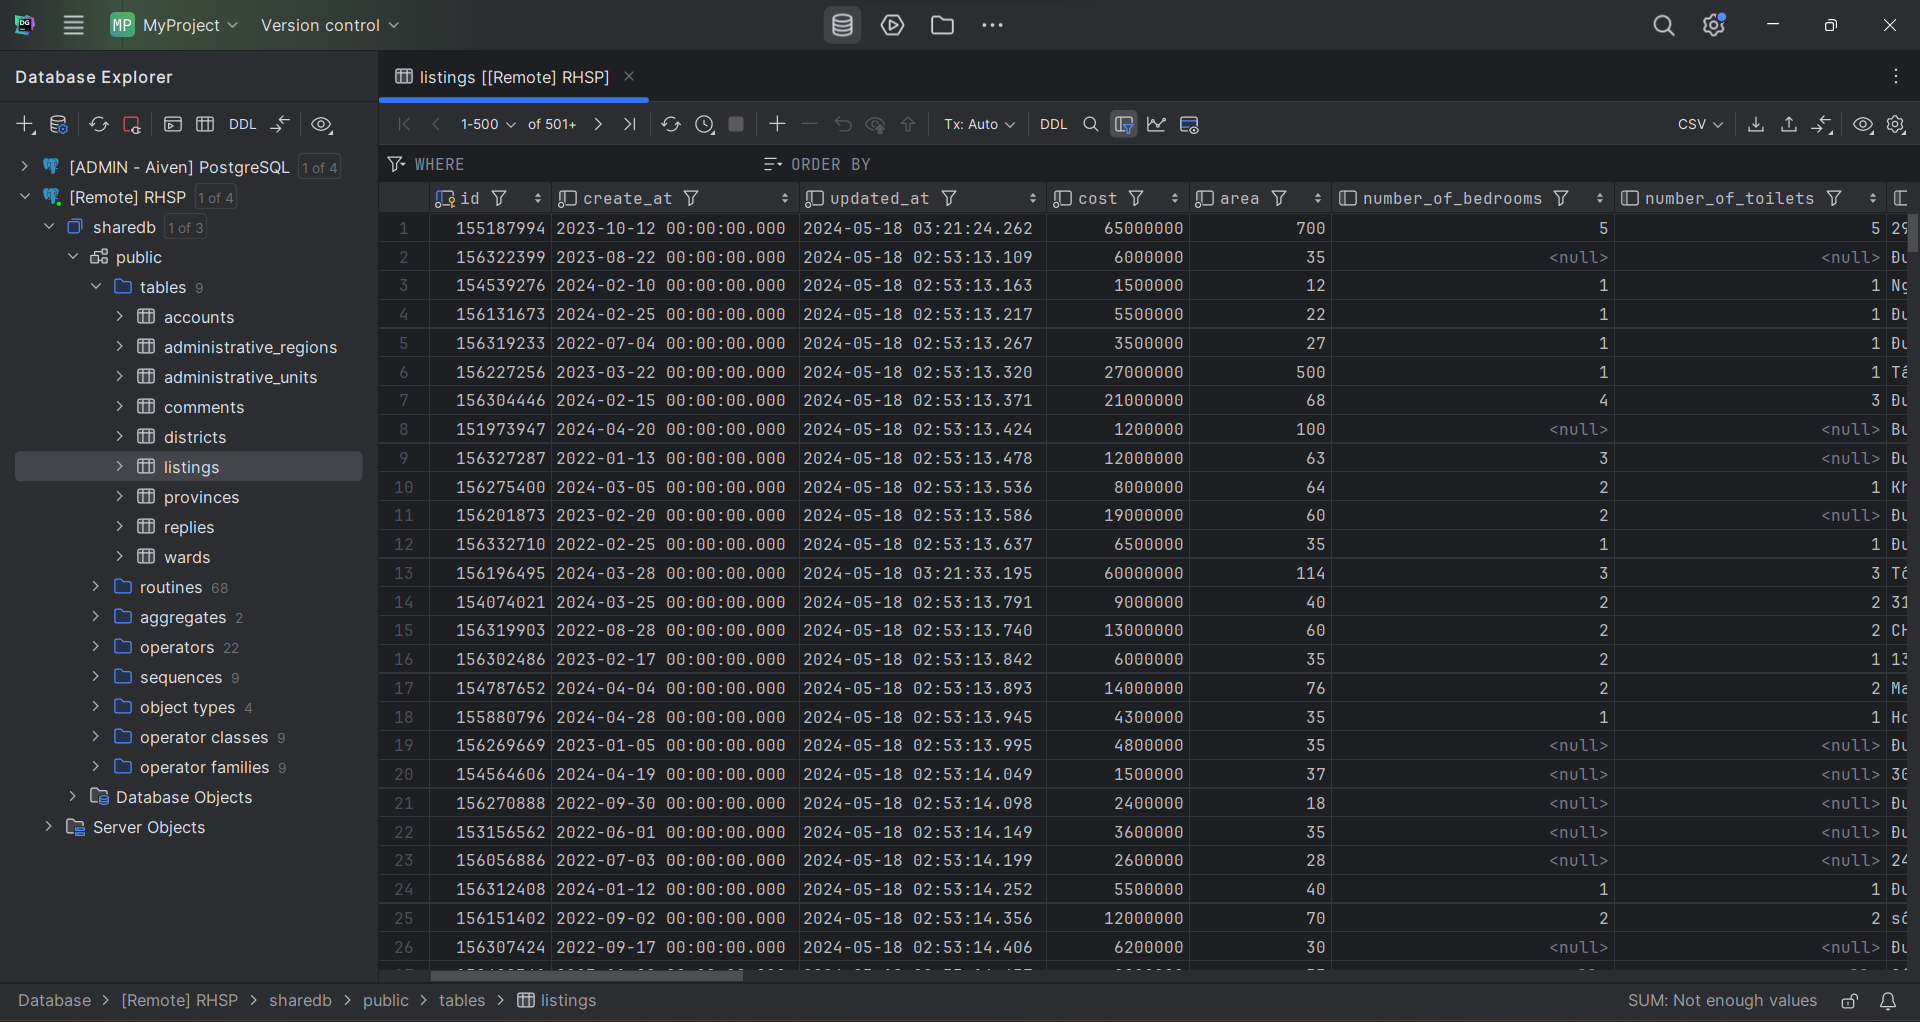
\includegraphics[width=1\textwidth]{Images/Database/DataGrip.png}
    \caption{Môi trường làm việc của DataGrip}
\end{figure}
\hspace*{1cm}
Để tạo ra thiết kế bảng cho cơ sở dữ liệu với công cụ \textit{DataGrip}, chúng ta chỉ cần nhấn chuột phải vào tên của \textit{database} hoặc \textit{schema} nằm ở cột bên trái của giao diện \textit{DataGrip}. Sau đó nhấn chọn \textit{Diagrams} và cuối cùng là nhấn chọn \textit{Show Diagram}, hoặc để đơn giản hơn, ta chỉ cần nhấn chọn chuột trái vào tên của \textit{database} hoặc \textit{schema} nằm ở cột bên trái của giao diện \textit{DataGrip}, sau đó nhấn tổ hợp phím \textit{Ctrl + Alt + Shift + U}. Sau khi thực hiện các bước trên, \textit{DataGrip} sẽ tự động tạo ra thiết kế bảng cho cơ sở dữ liệu mà ta đã chọn ở bước trên. Thiết kế bảng sẽ được hiển thị như hình ảnh bên dưới.
\begin{figure}[H]
    \centering
    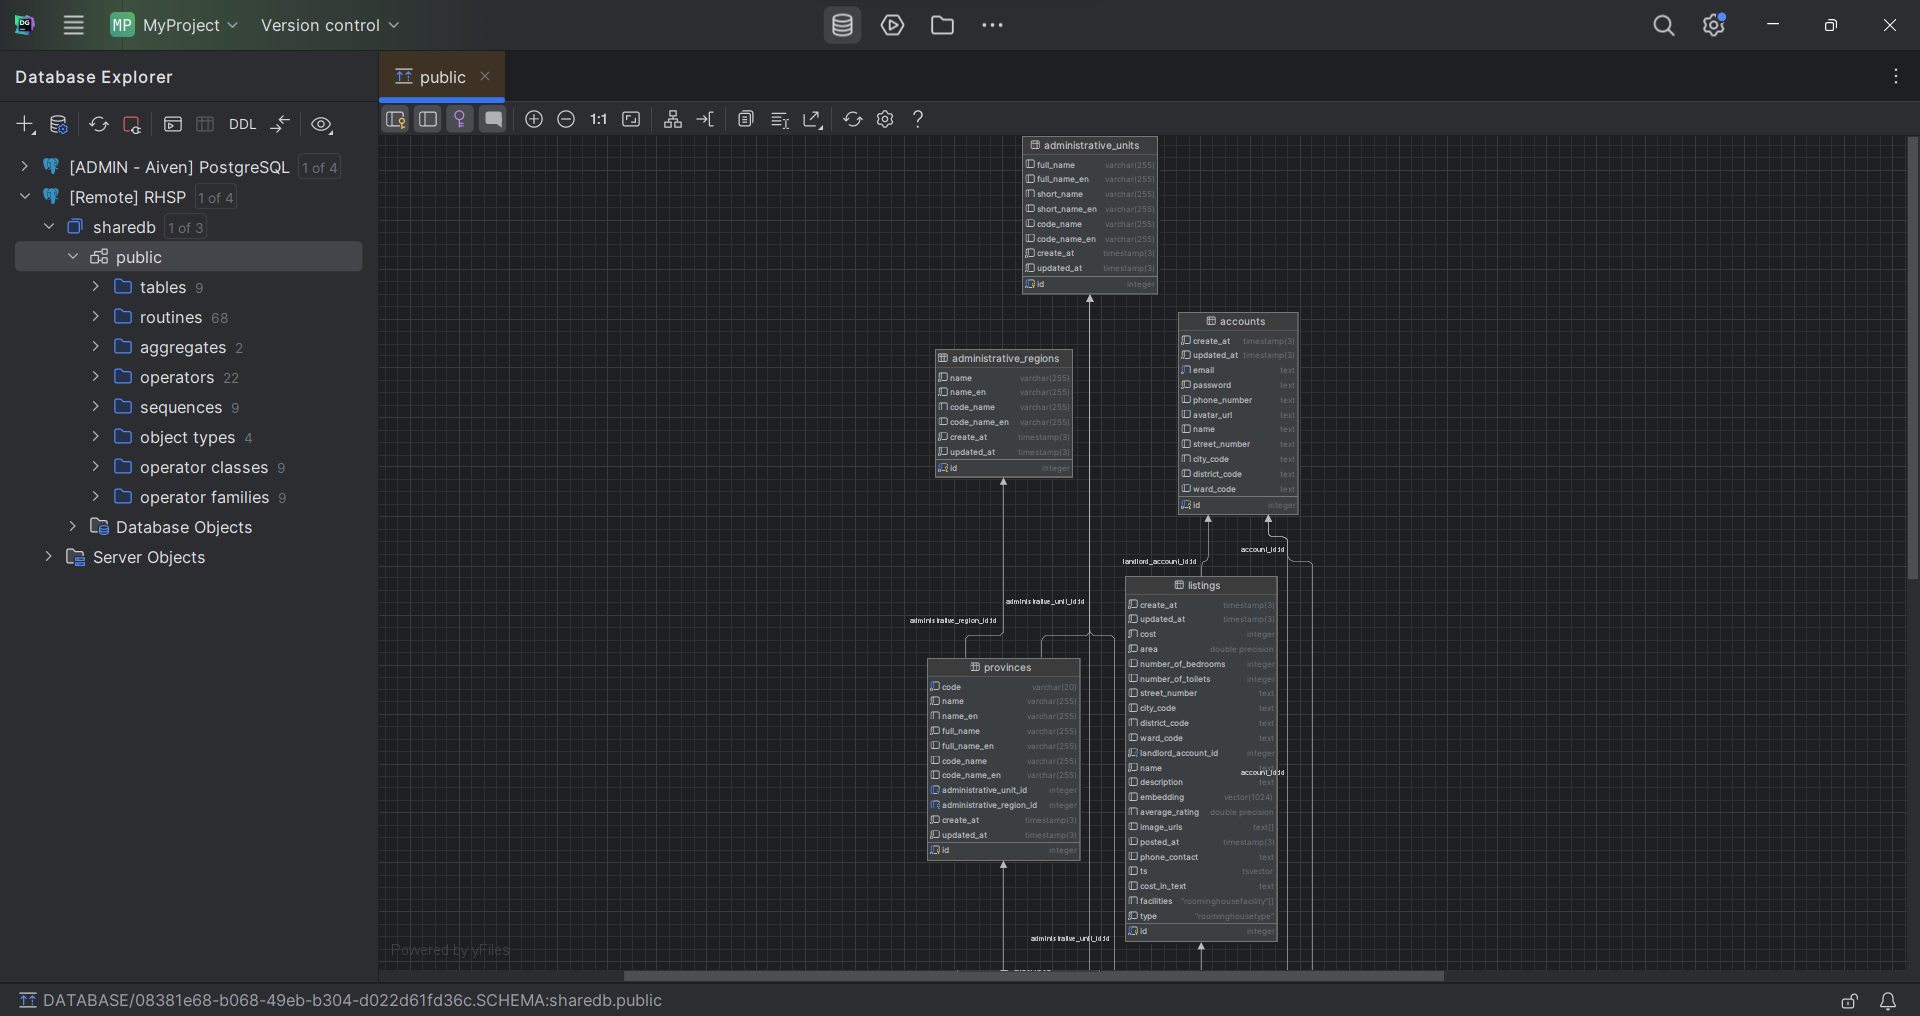
\includegraphics[width=1\textwidth]{Images/Database/ShowDiagram.png}
    \caption{Kết quả sau khi tạo thiết kế cơ sở dữ liệu trên DataGrip}
\end{figure}
\hspace*{1cm}
Do \textit{DataGrip} sinh ra thiết kế một cách tự động nên thiết kế ban đầu vẫn chưa thực sự trực quan. Ở bước này, ta cần căn chỉnh lại vị trí cho các bảng, cũng như điều chỉnh lại các đường mũi tên biểu thị cho mối quan hệ giữa các bảng với nhau để giúp cho thiết kế trở nên dễ quan sát một cách thuận tiện hơn và trực quan hơn. Sau khi đã căn chỉnh, kết quả sẽ cho ra như hình ảnh bên dưới
\begin{figure}[H]
    \centering
    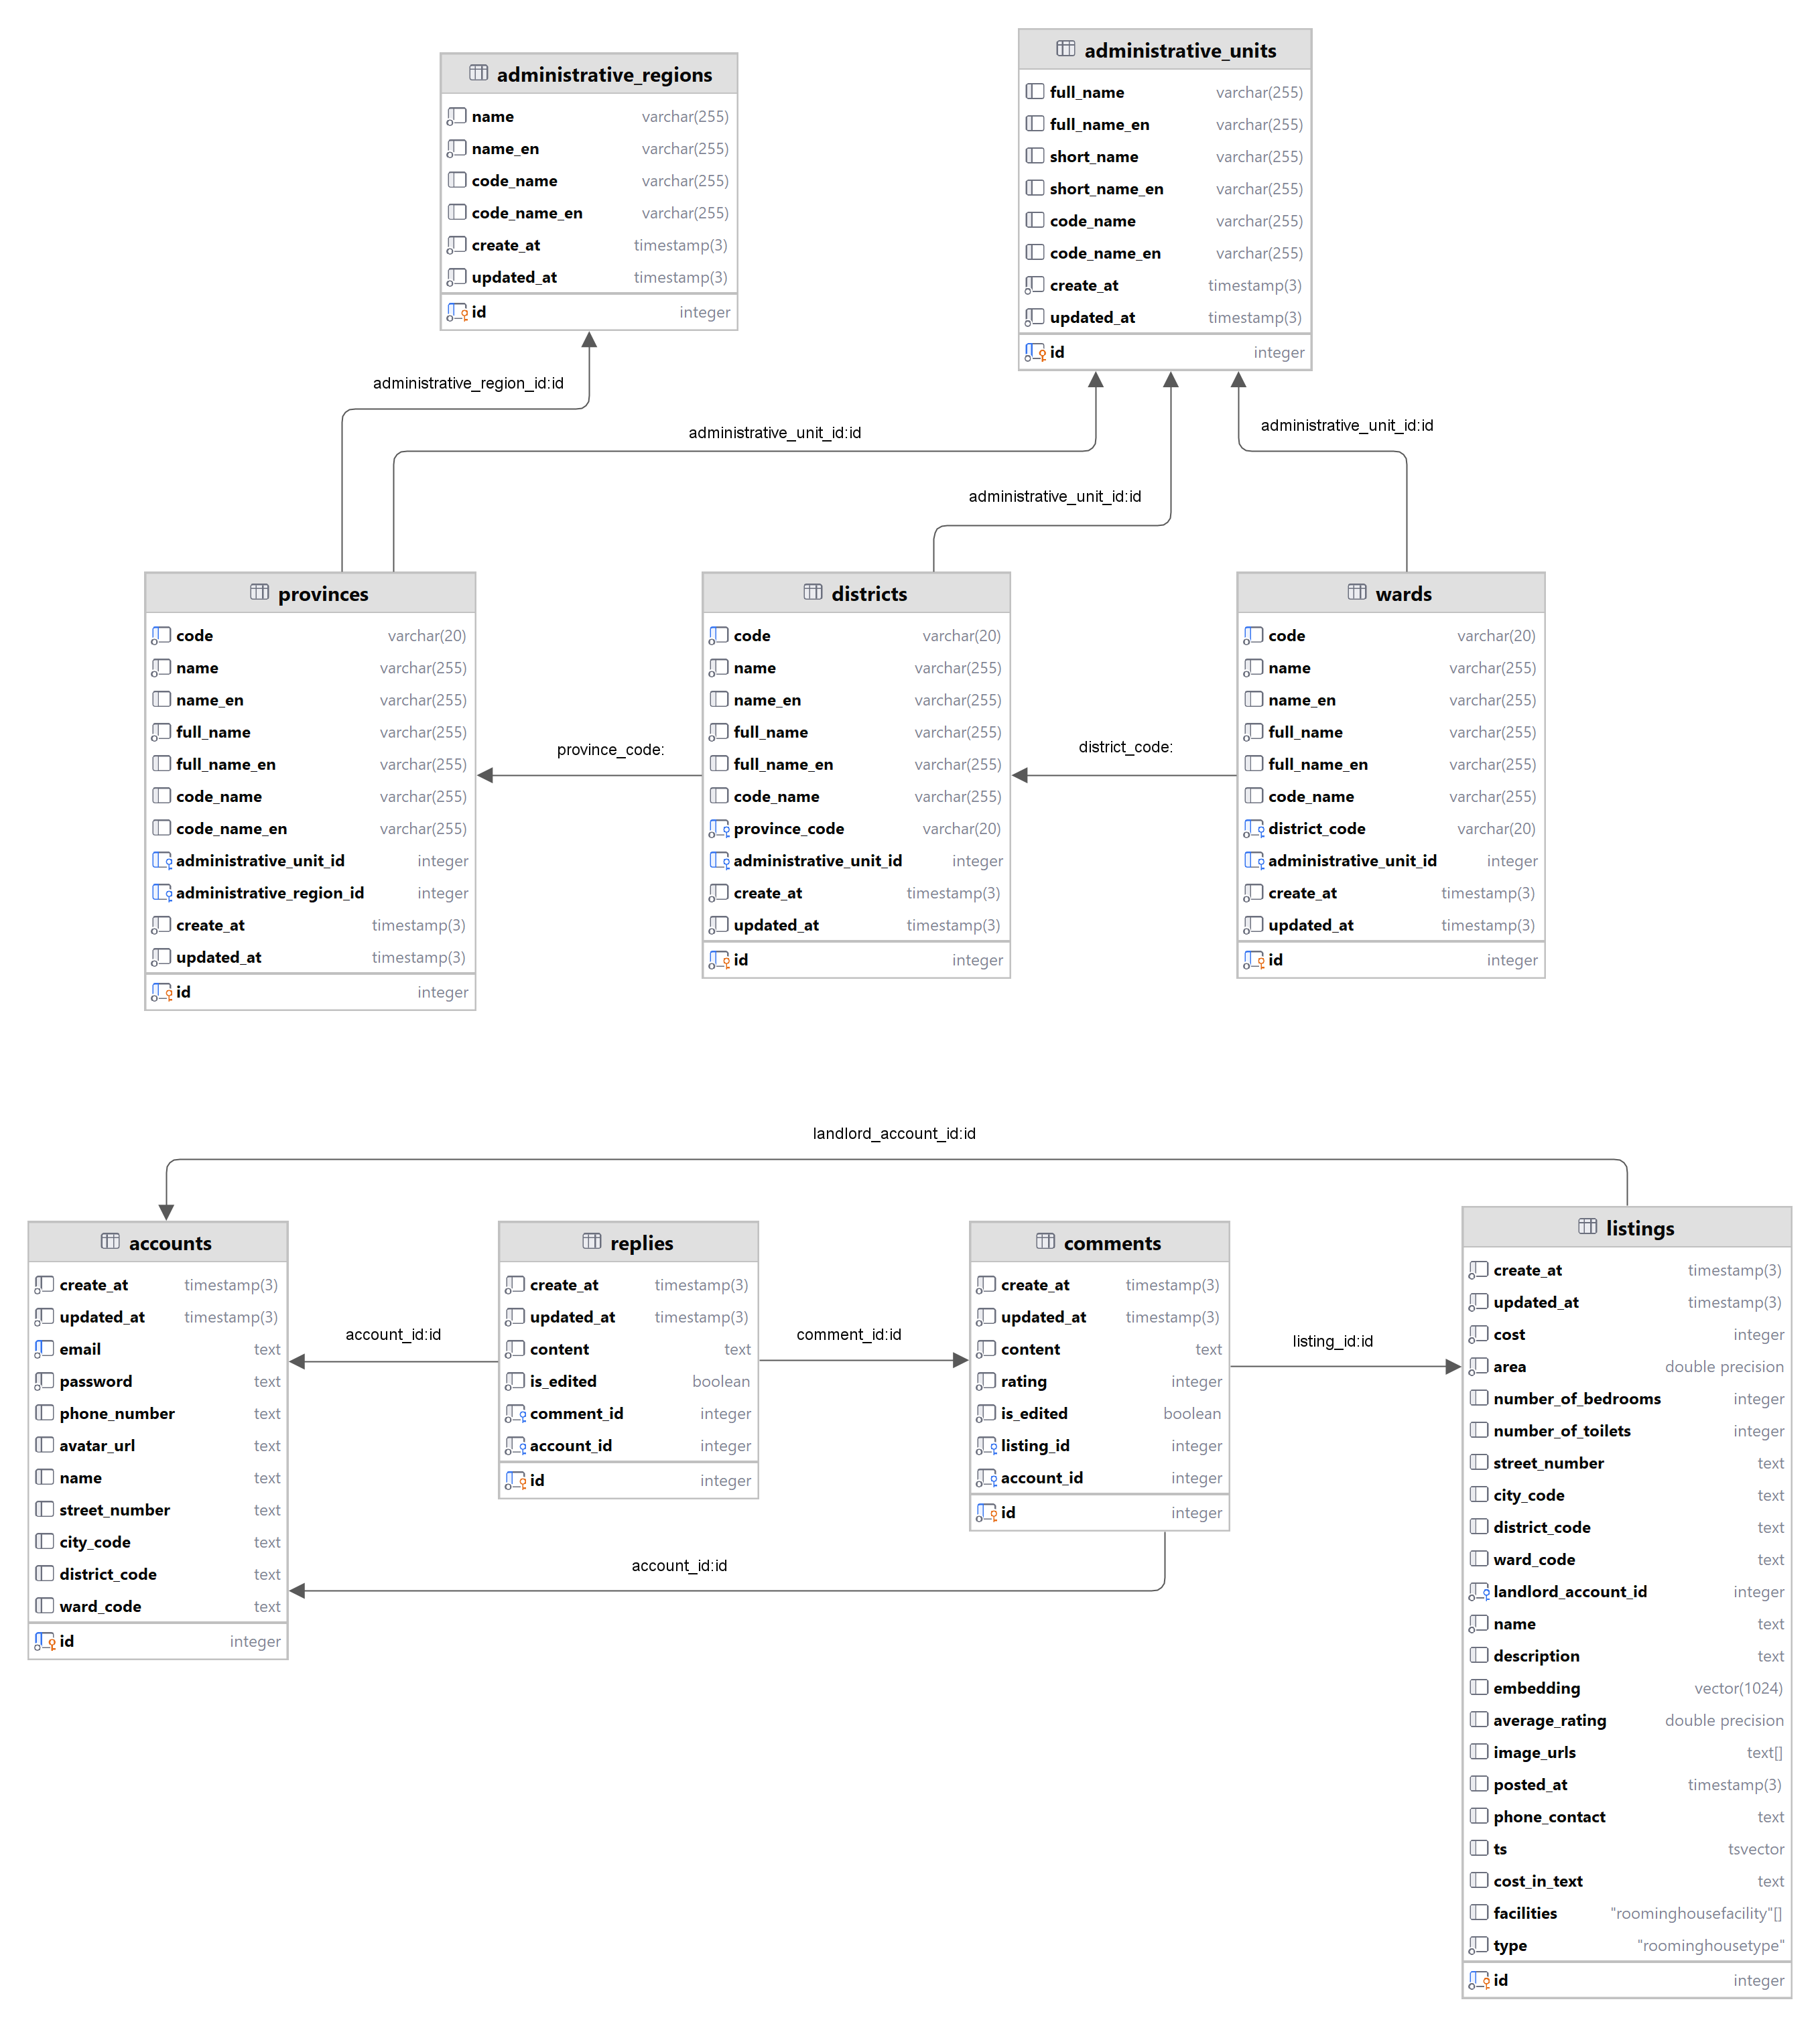
\includegraphics[width=0.98\textwidth]{Images/Database/Table.png}
    \caption{Thiết kế bảng cho cơ sở dữ liệu}
\end{figure}
\newpage
\subsection{Mô tả các bảng}
\subsubsection{Bảng administrative\_units}
\begin{center}
    \begin{longtblr}[caption={Bảng administrative\_units}]{
        colspec = { Q[m] Q[m] Q[c,m] X[m] },
        row{1} = {bg = yellow!75!black, fg = white, c},
        row{2 - 10} = {bg = yellow!10!white},
        vline{1, 5} = {2pt, yellow!75!black},
	hline{1, 2, 11} = {2pt, yellow!75!black},
        vline{2 - 4} = {dashed, yellow!75!black},
        hline{3 - 10} = {dashed, yellow!75!black},
	rows = {m},
    }
    \textbf{Thuộc tính } & \textbf{Kiểu} & \textbf{NULLABLE} & \textbf{Mô tả}
    \\
    \underline{\bf id} & integer & False & \textbf{Khóa chính}, thiết lập tự động tăng giá trị
    \\
    create\_at & timestamp(3) & False & Thời điểm khởi tạo dữ liệu, mặc định là \textit{now}
    \\
    update\_at & timestamp(3) & False & Thời điểm cuối cùng bản ghi cỏ thay đổi thuộc tính
    \\
    full\_name & varchar(100) & True & Tên đầy đủ của đơn vị hành chính
    \\
    full\_name\_en & varchar(100) & True & Tên đầy đủ của đơn vị hành chính bằng tiếng Anh
    \\
    short\_name & varchar(100) & True & Tên ngắn gọn của đơn vị hành chính
    \\
    short\_name\_en & varchar(100) & True & Tên ngắn gọn của đơn vị hành chính bằng tiếng Anh
    \\
    code\_name & varchar(100) & True & Tên chuẩn hóa của đơn vị hành chính
    \\
    code\_name\_en & varchar(100) & True & Tên chuẩn hóa của đơn vị hành chính bằng tiếng Anh
    \end{longtblr}
\end{center}
\subsubsection{Bảng administrative\_regions}
\begin{center}
    \begin{longtblr}[caption={Bảng administrative\_regions}]{
        colspec = { Q[m] Q[m] Q[c,m] X[m] },
        row{1} = {bg = yellow!75!black, fg = white, c},
        row{2 - 8} = {bg = yellow!10!white},
        vline{1, 5} = {2pt, yellow!75!black},
	hline{1, 2, 9} = {2pt, yellow!75!black},
        vline{2 - 4} = {dashed, yellow!75!black},
        hline{3 - 8} = {dashed, yellow!75!black},
	rows = {m},
    }
    \textbf{Thuộc tính } & \textbf{Kiểu} & \textbf{NULLABLE} & \textbf{Mô tả}
    \\
    \underline{\bf id} & integer & False & \textbf{Khóa chính}, thiết lập tự động tăng giá trị
    \\
    create\_at & timestamp(3) & False & Thời điểm khởi tạo dữ liệu, mặc định là \textit{now}
    \\
    update\_at & timestamp(3) & False & Thời điểm cuối cùng bản ghi cỏ thay đổi thuộc tính
    \\
    name & varchar(255) & True & Tên đầy đủ của vùng kinh tế - xã hội
    \\
    name\_en & varchar(255) & True & Tên đầy đủ của vùng kinh tế - xã hội bằng tiếng Anh
    \\
    code\_name & varchar(255) & True & Tên chuẩn hóa của  vùng kinh tế - xã hội
    \\
    code\_name\_en & varchar(255) & True & Tên chuẩn hóa của vùng kinh tế - xã hội bằng tiếng Anh
    \end{longtblr}
\end{center}
\subsubsection{Bảng province}
\begin{center}
    \begin{longtblr}[caption={Bảng province}]{
        colspec = { Q[m] Q[m] Q[c,m] X[m] },
        row{1} = {bg = yellow!75!black, fg = white, c},
        row{2 - 10} = {bg = yellow!10!white},
        vline{1, 5} = {2pt, yellow!75!black},
	hline{1, 2, 11} = {2pt, yellow!75!black},
        vline{2 - 4} = {dashed, yellow!75!black},
        hline{3 - 10} = {dashed, yellow!75!black},
	rows = {m},
    }
    \textbf{Thuộc tính } & \textbf{Kiểu} & \textbf{NULLABLE} & \textbf{Mô tả}
    \\
    \underline{\bf id} & integer & False & \textbf{Khóa chính}, thiết lập tự động tăng giá trị
    \\
    create\_at & timestamp(3) & False & Thời điểm khởi tạo dữ liệu, mặc định là \textit{now}
    \\
    update\_at & timestamp(3) & False & Thời điểm cuối cùng bản ghi cỏ thay đổi thuộc tính
    \\
    code & varchar(20) & False & Mã tỉnh / thành phố
    \\
    full\_name & varchar(255) & True & Tên đầy đủ của tỉnh / thành phố
    \\
    full\_name\_en & varchar(255) & True & Tên đầy đủ của tỉnh / thành phố bằng tiếng Anh
    \\
    code\_name & varchar(255) & True & Tên chuẩn hóa của tỉnh / thành phố
    \\
    administrative\_unit\_id & integer & False & \textit{Khóa ngoại}, tham chiếu đến \textit{id} của bảng \textbf{administrative\_units}
    \\
    administrative\_region\_id & integer & False & \textbf{Khóa ngoại}, tham chiếu đến \textit{id} của bảng \textit{administrative\_regions}
    \end{longtblr}
\end{center}
\newpage
\subsubsection{Bảng districts}
\begin{center}
    \begin{longtblr}[caption={Bảng districts}]{
        colspec = { Q[m] Q[m] Q[c,m] X[m] },
        row{1} = {bg = yellow!75!black, fg = white, c},
        row{2 - 10} = {bg = yellow!10!white},
        vline{1, 5} = {2pt, yellow!75!black},
	hline{1, 2, 11} = {2pt, yellow!75!black},
        vline{2 - 4} = {dashed, yellow!75!black},
        hline{3 - 10} = {dashed, yellow!75!black},
	rows = {m},
    }
    \textbf{Thuộc tính } & \textbf{Kiểu} & \textbf{NULLABLE} & \textbf{Mô tả}
    \\
    \underline{\bf id} & integer & False & \textbf{Khóa chính}, thiết lập tự động tăng giá trị
    \\
    create\_at & timestamp(3) & False & Thời điểm khởi tạo dữ liệu, mặc định là \textit{now}
    \\
    update\_at & timestamp(3) & False & Thời điểm cuối cùng bản ghi cỏ thay đổi thuộc tính
    \\
    code & varchar(20) & False & Mã quận / huyện và đơn vị hành chính tương đương
    \\
    full\_name & varchar(255) & True & Tên đầy đủ của quận / huyện và đơn vị hành chính tương đương
    \\
    full\_name\_en & varchar(255) & True & Tên đầy đủ của quận / huyện và đơn vị hành chính tương đương bằng tiếng Anh
    \\
    code\_name & varchar(255) & True & Tên chuẩn hóa của quận / huyện và đơn vị hành chính tương đương
    \\
    administrative\_unit\_id & integer & False & \textbf{Khóa ngoại}, tham chiếu đến trường \textit{id} của bảng \textit{administrative\_units}
    \\
    province\_code & varchar(20) & False & \textbf{Khóa ngoại}, tham chiếu đến trường \textit{code} của bảng \textit{provinces}
    \end{longtblr}
\end{center}
\subsubsection{Bảng wards}
\begin{center}
    \begin{longtblr}[caption={Bảng wards}]{
        colspec = { Q[m] Q[m] Q[c,m] X[m] },
        row{1} = {bg = yellow!75!black, fg = white, c},
        row{2 - 10} = {bg = yellow!10!white},
        vline{1, 5} = {2pt, yellow!75!black},
	hline{1, 2, 11} = {2pt, yellow!75!black},
        vline{2 - 4} = {dashed, yellow!75!black},
        hline{3 - 10} = {dashed, yellow!75!black},
	rows = {m},
    }
    \textbf{Thuộc tính } & \textbf{Kiểu} & \textbf{NULLABLE} & \textbf{Mô tả}
    \\
    \underline{\bf id} & integer & False & \textbf{Khóa chính}, thiết lập tự động tăng giá trị
    \\
    create\_at & timestamp(3) & False & Thời điểm khởi tạo dữ liệu, mặc định là \textit{now}
    \\
    update\_at & timestamp(3) & False & Thời điểm cuối cùng bản ghi cỏ thay đổi thuộc tính
    \\
    code & varchar(20) & False & Mã phường / xã và đơn vị hành chính tương đương
    \\
    full\_name & varchar(255) & True & Tên đầy đủ của phường / xã và đơn vị hành chính tương đương
    \\
    full\_name\_en & varchar(255) & True & Tên đầy đủ của phường / xã và đơn vị hành chính tương đương bằng tiếng Anh
    \\
    code\_name & varchar(255) & True & Tên chuẩn hóa của phường / xã và đơn vị hành chính tương đương
    \\
    administrative\_unit\_id & integer & False & \textit{Khóa ngoại}, tham chiếu đến trường \textbf{id} của bảng \textit{administrative\_units}
    \\
    district\_code & varchar(20) & False & \textit{Khóa ngoại}, tham chiếu đến trường \textbf{code} của bảng \textit{districts}
    \end{longtblr}
\end{center}
\subsubsection{Bảng accounts}
\begin{center}
    \begin{longtblr}[caption={Bảng accounts}]{
        colspec = { Q[m] Q[m] Q[c,m] X[m] },
        row{1} = {bg = yellow!75!black, fg = white, c},
        row{2 - 13} = {bg = yellow!10!white},
        vline{1, 5} = {2pt, yellow!75!black},
	hline{1, 2, 14} = {2pt, yellow!75!black},
        vline{2 - 4} = {dashed, yellow!75!black},
        hline{3 - 13} = {dashed, yellow!75!black},
	rows = {m},
    }
    \textbf{Thuộc tính } & \textbf{Kiểu} & \textbf{NULLABLE} & \textbf{Mô tả}
    \\
    \underline{\bf id} & int & False & \textbf{Khóa chính}, thiết lập tự động tăng giá trị
    \\
    create\_at & timestamp(3) & False & Thời điểm khởi tạo dữ liệu, mặc định là \textit{now}
    \\
    update\_at & timestamp(3) & False & Thời điểm cuối cùng bản ghi cỏ thay đổi thuộc tính
    \\
    email & text & False & Địa chỉ email của người dùng
    \\
    password & text & False & Mật khẩu của người dùng sau khi đã được băm
    \\
    name & text & True & Tên của người dùng
    \\
    avatar\_url & text & True & Đường dẫn tới file hình ảnh đại diện của người dùng
    \\
    phone\_number & text & True & Số điện thoại của người dùng
    \\
    street\_number & text & True & Số nhà và tên đường của địa chỉ người dùng
    \\
    city\_code & text & True & Mã tỉnh / thành phố của địa chỉ người dùng
    \\
    district\_code & text & True & Mã quận / huyện hoặc đơn vị hành chính tương đương của địa chỉ người dùng
    \\
    ward\_code & text & True & Mã phường / xã hoặc đơn vị hành chính tương đương của địa chỉ người dùng
    \\
    \end{longtblr}
\end{center}
\subsubsection{Bảng listings}
\begin{center}
    \begin{longtblr}[caption={Bảng listings}]{
        colspec = { Q[m] Q[m] Q[c,m] X[m] },
        row{1} = {bg = yellow!75!black, fg = white, c},
        row{2 - 22} = {bg = yellow!10!white},
        vline{1, 5} = {2pt, yellow!75!black},
	hline{1, 2, 23} = {2pt, yellow!75!black},
        vline{2 - 4} = {dashed, yellow!75!black},
        hline{3 - 22} = {dashed, yellow!75!black},
	rows = {m},
    }
    \textbf{Thuộc tính } & \textbf{Kiểu} & \textbf{NULLABLE} & \textbf{Mô tả}
    \\
    \underline{\bf id} & int & False & \textbf{Khóa chính}, thiết lập tự động tăng giá trị
    \\
    create\_at & timestamp(3) & False & Thời điểm khởi tạo dữ liệu, mặc định là \textit{now}
    \\
    update\_at & timestamp(3) & False & Thời điểm cuối cùng bản ghi cỏ thay đổi thuộc tính
    \\
    name & text & False & Tên của bài đăng tải nhà thuê
    \\
    type & rooming\_house\_type & False & Loại hình cho thuê, thuộc một
    trong các loại hình sau: \textit{Phòng trọ}, \textit{Căn hộ} hoặc \textit{Nhà đất}
    \\
    cost & integer & False & Giá tiền thuê của nhà thuê tính theo tháng
    \\
    area & double precision & False & Diện tích của nhà thuê
    \\
    number\_of\_bedrooms & integer & True & Số phòng ngủ của nhà thuê
    \\
    number\_of\_toilets & integer & True & Số nhà vệ sinh của nhà thuê
    \\
    street\_number & text & True & Số nhà và tên đường của địa chỉ nhà thuê
    \\
    city\_code & text & True & Mã tỉnh / thành phố của địa chỉ nhà thuê
    \\
    district\_code & text & True & Mã quận / huyện hoặc đơn vị hành chính tương đương của địa chỉ nhà thuê
    \\
    ward\_code & text & True & Mã phường / xã hoặc đơn vị hành chính tương đương của địa chỉ nhà thuê
    \\
    description & text & True & Mô tả ngắn về bài đăng tải nhà thuê
    \\
    image\_url & text & True & Đường dẫn tới các file hình ảnh của bài đẳng tải nhà thuê
    \\
    phone\_contact & text & True & Số điện thoại liên hệ của bài đăng tải nhà thuê
    \\
    facilities & rooming\_house\_facility & True & Các tiện ích của nhà thuê, các tiện ích đó bao gồm: \textit{Tivi}, \textit{Camera giám sát}, \textit{Cảm biến}, \textit{Tủ lạnh}, \textit{Máy giặt}, \textit{Điều hòa}
    \\
    average\_rating & text & True & Điểm đánh giá trung bình dựa trên các bình luận của bài đăng tải nhà thuê
    \\
    cost\_in\_text & text & True & Giá thuê theo tháng được phiên âm thành tiếng Việt, được sử dụng trong mô hình tìm kiếm Hybrid
    \\
    ts & tsvector & True & Lưu trữ \textit{indexes} của các từ trong bài đăng, được sử dụng trong \textit{full-text search}
    \\
    embedding & vector(1024) & True & Vector có 1024 do mô hình \textit{vector embeeding} sinh ra để biểu thị cho ngữ nghĩa của bài đăng tải nhà trọ, được sử dụng trong \textit{semantic search}
    \end{longtblr}
\end{center}
\subsubsection{Bảng comments}
\begin{center}
    \begin{longtblr}[caption={Bảng comments}]{
        colspec = { Q[m] Q[m] Q[c,m] X[m] },
        row{1} = {bg = yellow!75!black, fg = white, c},
        row{2 - 9} = {bg = yellow!10!white},
        vline{1, 5} = {2pt, yellow!75!black},
	hline{1, 2, 10} = {2pt, yellow!75!black},
        vline{2 - 4} = {dashed, yellow!75!black},
        hline{3 - 9} = {dashed, yellow!75!black},
	rows = {m},
    }
    \textbf{Thuộc tính } & \textbf{Kiểu} & \textbf{NULLABLE} & \textbf{Mô tả}
    \\
    \underline{\bf id} & int & False & \textbf{Khóa chính}, thiết lập tự động tăng giá trị
    \\
    create\_at & timestamp(3) & False & Thời điểm khởi tạo dữ liệu, mặc định là \textit{now}
    \\
    update\_at & timestamp(3) & False & Thời điểm cuối cùng bản ghi cỏ thay đổi thuộc tính
    \\
    content & text & False & Nội dung bình luận của người dùng
    \\
    rating & integer & False & Số điểm đánh giá của người dùng đối với nhà thuê
    \\
    is\_edited & boolean & False & Biểu thị cho thấy bình luận đã được chỉnh sửa hay chưa, giá trị mặc định là \textit{false}
    \\
    listing\_id & integer & False & \textbf{Khóa ngoại}, tham chiếu đến trường \textit{id} của bảng \textit{listings}
    \\
    account\_id & integer & False & \textbf{Khóa ngoại}, tham chiếu đến trường \textit{id} của bảng \textit{accounts}
    \end{longtblr}
\end{center}
\subsubsection{Bảng replies}
\begin{center}
    \begin{longtblr}[caption={Bảng replies}]{
        colspec = { Q[m] Q[m] Q[c,m] X[m] },
        row{1} = {bg = yellow!75!black, fg = white, c},
        row{2 - 8} = {bg = yellow!10!white},
        vline{1, 5} = {2pt, yellow!75!black},
	hline{1, 2, 9} = {2pt, yellow!75!black},
        vline{2 - 4} = {dashed, yellow!75!black},
        hline{3 - 8} = {dashed, yellow!75!black},
	rows = {m},
    }
    \textbf{Thuộc tính } & \textbf{Kiểu} & \textbf{NULLABLE} & \textbf{Mô tả}
    \\
    \underline{\bf id} & int & False & \textbf{Khóa chính}, thiết lập tự động tăng giá trị
    \\
    create\_at & timestamp(3) & False & Thời điểm khởi tạo dữ liệu, mặc định là \textit{now}
    \\
    update\_at & timestamp(3) & False & Thời điểm cuối cùng bản ghi cỏ thay đổi thuộc tính
    \\
    content & text & False & Nội dung trả lời phản hồi của bình luận của người dùng
    \\
    is\_edited & boolean & False & Biểu thị cho thấy phản hồi bình luận đã được chỉnh sửa hay chưa, giá trị mặc định là \textit{false}
    \\
    comment\_id & integer & False & \textbf{Khóa ngoại}, tham chiếu đến trường \textit{id} của bảng \textit{comments}
    \\
    account\_id & integer & False & \textbf{Khóa ngoại}, tham chiếu đến trường \textit{id} của bảng \textit{accounts}
    \end{longtblr}
\end{center}
\section{KIẾN TRÚC HỆ THỐNG}
\begin{figure}[h]
    \centering
    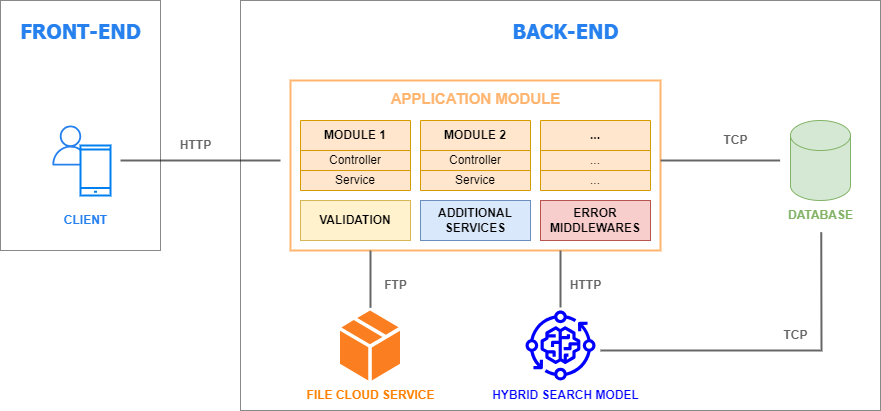
\includegraphics[width=1\textwidth]{Images/SystemArchitecture.png}
    \caption{Sơ đồ kiến trúc của ứng dụng Housernet}
\end{figure}
Ứng dụng Housernet sẽ được chia ra làm hai phần độc lập với nhau là \textit{front-end} và \textit{back-end}, trong đó phía \textit{client} sẽ gọi đến các chức năng của \textit{server} thông qua giao thức \textit{HTTP}, và phía \textit{server} sẽ được tổ chức thành các thành phần cụ thể khác nhau để xử lý cho các chức năng khác nhau. Một cách cụ thể hơn, kiến trúc này sẽ được chia ra thành các phần chính bao gồm:
\begin{itemize}
    \item \textit{Application module:} Đây là thành phần chính của \textit{back-end}, chứa đựng toàn bộ các chức năng nghiệp vụ của ứng dụng. Thành phần này sẽ chịu trách nhiệm chính trong việc giao tiếp với phía \textit{front-end} cho các yêu cầu xử lý từ phía người dùng. Mỗi chức năng sẽ được tổ chức thành mỗi \textit{module}, trong mỗi \textit{module} sẽ bao gồm \textit{controller} để tiếp nhận yêu cầu từ phía \textit{client} và thực hiện gọi phương thức phù hợp với yêu cầu nghiệp vụ ở tầng \textit{service}, như thế thành phần \textit{service} là nơi chứa đựng xử lý \textit{logic} chính cho chức năng đó. Bên cạnh đó, \textit{application module} còn có các thành phần xử lý khác bao gồm \textit{validation} - chịu trách nhiệm để kiểm tra tính hợp lệ của các yêu cầu gửi lên từ phía \textit{client}, \textit{additional services} - nơi tích hợp các chức năng từ bên thứ ba, bao gồm dịch vụ để kết nối với cơ sở dữ liệu thông qua \textit{ORM}, dịch vụ lưu trữ \textit{file} đám mây, dịch vụ \textit{vector embedding} cho văn bản, và cuối cùng là thành phần \textit{error middlewares} - chịu trách nhiệm bắt các lỗi liên quan đến thao tác với cơ sở dữ liệu.
    \item \textit{File cloud service:} Đây là nơi cung cấp dịch vụ lưu trữ \textit{file} đám mây, dịch vụ này được kết nối với \textit{application module} thông qua giao thức \textit{FTP}. Dịch vụ này được sử dụng cho mục đích tải \textit{file} do người dùng tải lên và lưu trữ, sau đó dịch vụ này sẽ trả về địa chỉ \textit{URL} để người dùng có thể truy cập trực tiếp vào \textit{file} tương ứng.
    \item \textit{Hybrid search model:} Thành phần này cung cấp chức năng tìm kiếm kết hợp, được xem như là tính năng chính cho ứng dụng. Thành phần này được triển khai tách biệt hoàn toàn so với \textit{application module} và sẽ cung cấp \textit{API} để cho \textit{application module} có thể gọi tới khi có yêu cầu liên quan đến chức năng tìm kiếm kết hợp. Ngoài ra thành phần này cũng giao tiếp với cơ sở dữ liệu bằng giao thức \textit{TCP} để có thể truy vấn kết quả tìm kiếm từ cơ sở dữ liệu ứng với yêu cầu đầu vào của người dùng.
    \item \textit{Database:} Thành phần này là nơi để triển khai cơ sở dữ liệu cho toàn bộ chức năng của ứng dụng, thành phần này có thể giao tiếp với thành phần \textit{application module} và thành phần \textit{hybrid search model} thông qua giao thức \textit{TCP}. Để có thể thực hiện chức năng tìm kiếm ngữ nghĩa, cơ sở dữ liệu phải có khả năng tích hợp \textit{vector database extension}. Nhờ đó mà cơ sở dữ liệu có khả năng lưu trữ dữ liệu ở kiểu \textit{vector} cũng như cho phép các truy vấn dựa trên \textit{vector}.
\end{itemize}
\section{THIẾT KẾ UI/UX CHO ỨNG DỤNG}
\subsection{Màn hình đăng nhập và đăng ký tài khoản}
Khi lần đầu vào ứng dụng, người dùng cần phải đăng nhập vào tài khoản đã được tạo. Người dùng cần nhập tên đăng nhập và mật khẩu của họ để xác thực, hoặc họ có thể đăng nhập thông qua bên thứ ba là Facebook, Google hoặc là Apple ID.\\
Nếu người dùng vẫn chưa có tài khoản, họ có thể đăng ký bằng cách ấn vào nút "Đăng ký" để được điều hướng sang giao diện đăng ký tài khoản. Sau khi người dùng đã đăng ký thành công tài khoản, ứng dụng sẽ điều hướng sang trang nhập thông tin cá nhân. Người dùng có thể nhập các trường như họ và tên, số điện thoại, địa chỉ hoặc là chọn nút "Bỏ qua" để tạm thời không nhập các thông tin này.
\begin{figure}[!htb]
\centering
   \begin{minipage}{0.32\textwidth}
     \centering
     
\includegraphics[width=1\linewidth]{Images/UI figma/Signup 1.png}
     \caption{Giao diện đăng ký với tài khoản và mật khẩu}
   \end{minipage}\hfill
   \begin{minipage}{0.32\textwidth}
     \centering
     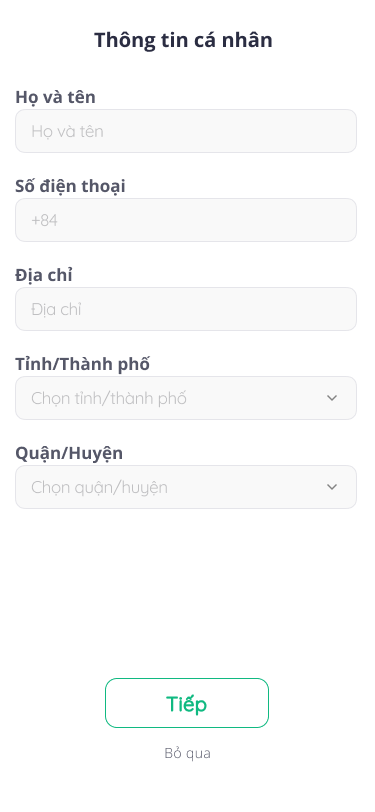
\includegraphics[width=1\linewidth]{Images/UI figma/Signup 2.png}
     \caption{Giao diện cung cấp thông tin cá nhân đăng ký}
   \end{minipage}\hfill
   \begin{minipage}{0.32\textwidth}
     \centering
     
\includegraphics[width=1\linewidth]{Images/UI figma/Login}
     \caption{Giao diện đăng nhập}
   \end{minipage}
\end{figure}
\newpage
\subsection{Màn hình quên mật khẩu}
Housernet cung cấp chức năng đặt lại mật khẩu trong trường hợp người dùng quên mật khẩu. Người dùng có thể đặt lại mật khẩu bằng cách ấn vào chữ "Quên mật khẩu" trong màn hình đăng nhập.
\begin{figure}[H]
    \centering
    
\includegraphics[width=0.33\textwidth]{Images/UI figma/Reset Password.png}
    \caption{Giao diện đặt lại mật khẩu}
\end{figure}
\newpage
\subsection{Màn hình chính}
Màn hình chính sẽ cung cấp các chức năng chính như:
\begin{itemize}
    \item Hiển thị danh sách nhà ở gần vị trí người dùng cung cấp
    \item Hiển thị danh sách nhà phù hợp với người dùng
    \item Tìm kiếm nhà bằng từ khóa như tên hoặc địa chỉ
    \item Cung cấp bộ lọc các nhà thỏa điều kiện.
\end{itemize}
Ngoài ra, tại góc dưới của màn hình chính còn có một thanh điều hướng có chức năng di chuyển đến các màn hình cài đặt và tài khoản.
\begin{figure}[H]
    \centering
    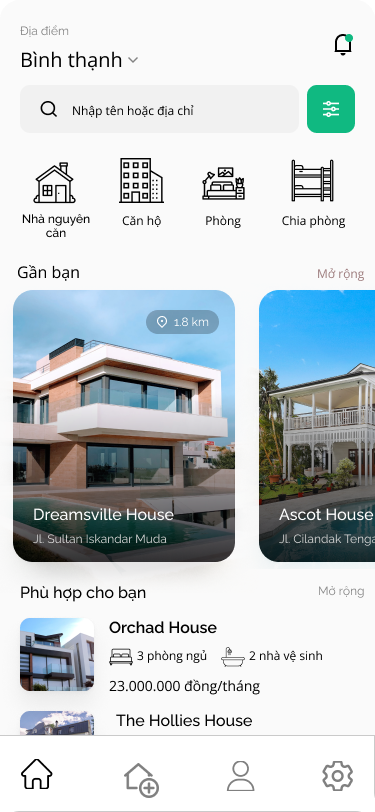
\includegraphics[width=0.33\textwidth]{Images/UI figma/Full home screen.png}
    \caption{Giao diện màn hình chính}
\end{figure}
\newpage
\subsection{Bộ lọc tìm kiếm nhà trọ}
Người dùng có thể sử dụng bộ lọc để lọc ra các kết quả cho nhà phù hợp điều kiện. Để có thể dùng bộ lọc, người dùng cần ấn vào nút lọc nằm cạnh bên phải thanh tìm kiếm tại màn hình chính. Bộ lọc bao gồm:
\begin{itemize}
    \item Loại, diện tích, số phòng: có thể ấn chọn 1 trong 4 loại
    \item Khu vực: Chọn khu vực như tỉnh/thành, quận/huyện hoặc phường/xã
    \item Giá: có thể kéo để chọn khoảng giá phù hợp
    \item Tiện ích: có thể chọn 1 hoặc nhiều tiện ích
\end{itemize}
\begin{figure}[!htb]
\centering
   \begin{minipage}{0.32\textwidth}
     \centering
     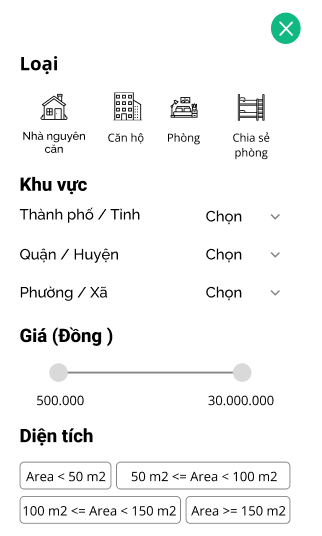
\includegraphics[width=1\linewidth]{Images/UI figma/Frame 1.png}
     \caption{Giao diện bộ lọc tìm kiếm nhà trọ}
   \end{minipage}\hspace{1cm}
   \begin{minipage}{0.32\textwidth}
     \centering
     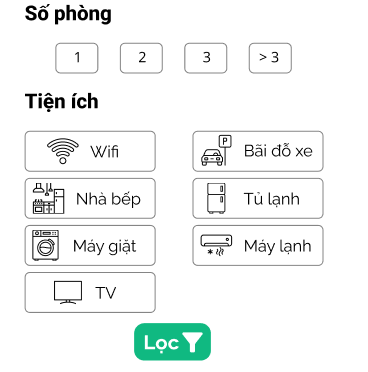
\includegraphics[width=1\linewidth]{Images/UI figma/Frame 2.png}
     \caption{Giao diện bộ lọc tìm kiếm nhà trọ (tiếp theo)}
   \end{minipage}
\end{figure}
\newpage
\subsection{Màn hình hồ sơ người dùng}
Người dùng có thể di chuyển đến màn hình tài khoản thông qua thanh điều hướng phía dưới trang chính. Tại đây người dùng có thể xem và điều chỉnh thông tin cá nhân hoặc là đăng xuất.
\begin{figure}[!htb]
    \centering
    \begin{minipage}{0.32\textwidth}
     \centering
     
\includegraphics[width=1.06\linewidth]{Images/UI figma/Profile.png}
     \caption{Giao diện hồ sơ người dùng}
    \end{minipage}\hspace{1cm}
    \begin{minipage}{0.32\textwidth}
     \centering
     
\includegraphics[width=1\linewidth]{Images/UI figma/Profile - Detail.png}
     \caption{Giao diện hồ sơ người dùng và thông tin cá nhân}
    \end{minipage}
\end{figure}
\newpage
\subsection{Đăng tải nhà trọ}
Chủ trọ có thể đăng tải nhà trọ để công khai thông tin nhà trọ lên ứng dụng bằng cách ấn vào nút "Đăng tải" tại giao diện quản lý nhà trọ. Để đăng tải, chủ trọ có thể chọn một nhà trọ đã có sẵn và ấn nút "Tiếp", lúc này ứng dụng sẽ tự động điền các thông tin đã có sẵn của nhà trọ và chủ trọ có thể sửa lại hoặc thêm các thông tin thêm như hình ảnh hoặc các tiện ích của nhà trọ. Sau khi chủ trọ ấn nút "Đăng tải" thì ứng dụng sẽ hiển thị thông báo thành công và chủ trọ có thể ấn nút "Quay về" để trở về màn hình chính.
\begin{figure}[!htb]
\centering
   \begin{minipage}{0.32\textwidth}
     \centering
     
\includegraphics[width=1\linewidth]{Images/UI figma/Upload Rooming House 1.png}
     \caption{Giao diện chọn danh sách nhà trọ có sẵn}
   \end{minipage}\hfill
   \begin{minipage}{0.32\textwidth}
     \centering
     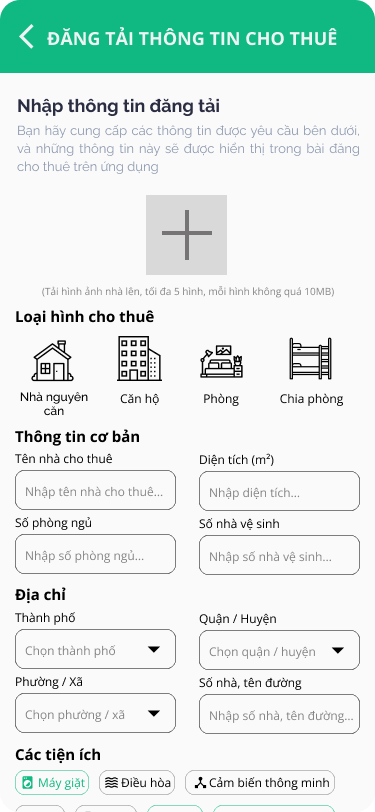
\includegraphics[width=1\linewidth]{Images/UI figma/Upload Rooming House 2.png}
     \caption{Giao diện nhập thông tin đăng tải nhà trọ}
   \end{minipage}\hfill
   \begin{minipage}{0.32\textwidth}
     \centering
     
\includegraphics[width=1\linewidth]{Images/UI figma/Upload Rooming House 3.png}
     \caption{Giao diện đăng tải nhà trọ thành công}
   \end{minipage}
\end{figure}
\newpage
\subsection{Quản lý nhà trọ}
Người dùng có thể di chuyển sang màn hình này thông qua thanh điều hướng phía dưới màn hình chính. Tại đây, người dùng có thể xem danh sách cái nhà đã đăng bài và có thể thao tác chỉnh sửa cũng như gỡ bỏ bài đăng đó. Ngoài ra người dùng còn có thể tạo bài đăng nhà trọ bằng cách ấn vào nút "Đăng tải" hoặc thêm một nhà trọ mới bằng nút "Thêm nhà trọ".
\begin{figure}[!htb]
\centering
   \begin{minipage}{0.32\textwidth}
     \centering
     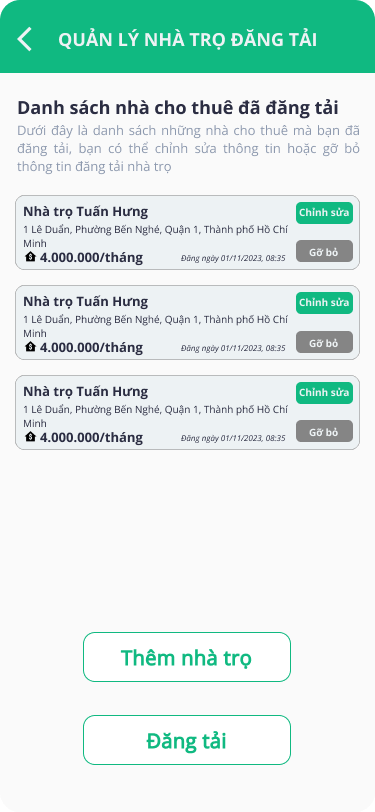
\includegraphics[width=1\linewidth]{Images/UI figma/Upload Rooming House 5.png}
     \caption{Giao diện chọn danh sách nhà trọ đã đăng}
   \end{minipage}\hfill
   \begin{minipage}{0.32\textwidth}
     \centering
     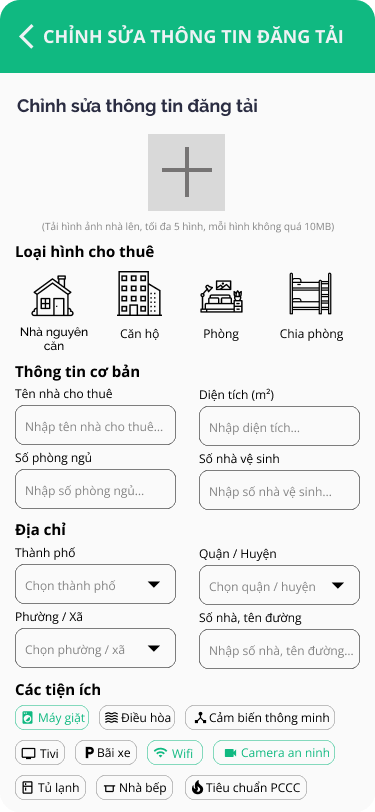
\includegraphics[width=1\linewidth]{Images/UI figma/Upload Rooming House 7.png}
     \caption{Giao diện chỉnh sửa thông tin đăng tải nhà trọ}
   \end{minipage}\hfill
   \begin{minipage}{0.32\textwidth}
     \centering
     
\includegraphics[width=1\linewidth]{Images/UI figma/Upload Rooming House 6.png}
     \caption{Giao diện chỉnh sửa nhà trọ thành công}
   \end{minipage}
\end{figure}


\section{CÔNG NGHỆ HIỆN THỰC}
\subsection{TSVector}
\subsubsection{Tổng quan}
\hspace*{1cm} TSvector là một kiểu dữ liệu trong PostgreSQL được sử dụng để lưu trữ các từ khóa được tối ưu hóa cho tìm kiếm toàn văn bản (FTS). Nó được tạo ra từ một chuỗi văn bản, nơi chuỗi văn bản đó được phân tích thành các từ khóa, loại bỏ các từ dừng (stop words) và sau đó sắp xếp theo thứ tự từ điển.
\subsubsection{Các tính năng nổi bật}
TSVector được sử dụng khá phổ biến nhờ vào các tính năng như sau:
\begin{itemize}
    \item Tìm kiếm toàn văn bản: TSvector cho phép tìm kiếm toàn bộ văn bản trong một cột, thay vì chỉ tìm kiếm các từ khóa khớp chính xác. Thông qua đó giúp tìm thấy các tài liệu có liên quan đến truy vấn , ngay cả khi chúng không chứa tất cả các từ khóa chính xác đã tìm kiếm.
    \item Hỗ trợ nhiều ngôn ngữ: TSvector hỗ trợ nhiều ngôn ngữ khác nhau, bao gồm tiếng Việt. Điều này giúp người dùng có thể tìm kiếm văn bản bằng ngôn ngữ mà người đó thông thạo , hiểu sâu nhất.
    \item Hỗ trợ nhiều loại truy vấn: TSvector hỗ trợ nhiều loại truy vấn khác nhau, bao gồm truy vấn AND, OR, NOT, gần đúng và truy vấn theo tiền tố. Hỗ trợ tìm kiếm văn bản một cách linh hoạt hơn.
\end{itemize}
\begin{figure}[H]
    \centering
    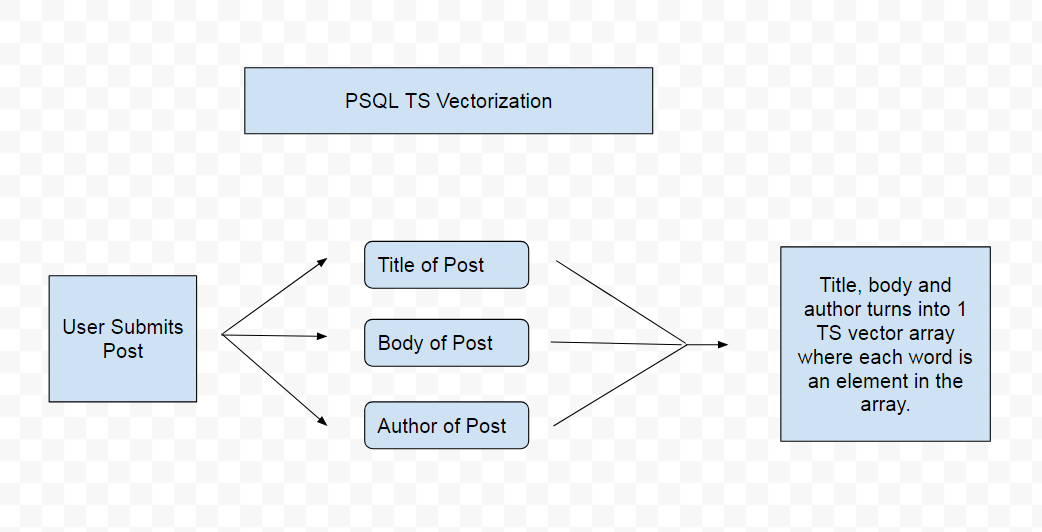
\includegraphics[width=0.8\textwidth]{Images/technology/TSVector.png}
    \caption{Nguyên lí hoạt động của TSVector}
\end{figure}
\subsubsection{Phân tích ưu và nhược điểm}
\textbf{Ưu điểm}
\begin{itemize}
    \item Tăng tốc độ tìm kiếm: TSvector sử dụng các kỹ thuật lập chỉ mục để tăng tốc độ tìm kiếm. Do vậy có thể tìm thấy kết quả nhanh hơn, ngay cả khi đang tìm kiếm trong một tập dữ liệu lớn.
    \item Sử dụng từ đồng nghĩa: TSvector có thể sử dụng từ đồng nghĩa bằng cách khai báo để tìm kiếm các tài liệu có chứa các từ khóa tương tự như truy vấn.
    \item Phân tích cú pháp: TSvector có thể phân tích cú pháp văn bản để hiểu rõ hơn về ý nghĩa của nó.
\end{itemize}
\textbf{Nhược điểm}
\begin{itemize}
    \item Khá tốn kém: cần phải có một tập dữ liệu lớn để sử dụng cho TSvector. Điều này là do TSvector sử dụng các kỹ thuật lập chỉ mục để tăng tốc độ tìm kiếm, mà các kỹ thuật lập chỉ mục này có thể tốn nhiều dung lượng lưu trữ.
    \item Độ phức tạp cao : Có thể có độ phức tạp cao khi sử dụng nếu bạn cần thực hiện các truy vấn phức tạp, do TSvector hỗ trợ nhiều loại truy vấn khác nhau, và mỗi loại truy vấn có cú pháp riêng.
    \item Kết quả không có độ chính xác cao : kết quả không chính xác nếu có một tập dữ liệu có chất lượng kém. TSVector hoạt động dựa vào các kỹ thuật lập chỉ mục để tìm kiếm, mà các kỹ thuật lập chỉ mục này có thể không chính xác nếu văn bản trong tập dữ liệu bị lỗi hoặc không chính xác.
\end{itemize}
\subsection{PgVector}
\subsubsection{Tổng quan}
Pgvector là một thư viện mở rộng dựa trên PostgreSQL nhằm cung cấp các chức năng mạnh mẽ để làm việc với vectơ trong không gian đa chiều, đồng thời giới thiệu một kiểu dữ liệu chuyên dụng, toán tử và hàm cho phép lưu trữ, thao tác và phân tích dữ liệu vectơ hiệu quả trực tiếp trong cơ sở dữ liệu PostgreSQL.
\subsubsection{Các tính năng nổi bật}
\begin{itemize}
    \item Lưu trữ vectơ: cung cấp một kiểu dữ liệu mới để lưu trữ vectơ trong PostgreSQL. Loại dữ liệu này được tối ưu hóa để lưu trữ vectơ hiệu quả và có thể được sử dụng để lưu trữ các vectơ có độ dài khác nhau.
    \item Thao tác vectơ: bao gồm một loạt các toán tử và hàm cho phép thao tác vectơ, chẳng hạn như cộng, trừ, nhân và chia. Các toán tử và hàm được tối ưu hóa để thực hiện hiệu quả và có thể được sử dụng để thực hiện các phép tính vectơ phức tạp.
    \item Phân tích vectơ: tích hợp một số hàm cho phép phân tích dữ liệu vectơ, chẳng hạn như tính toán độ dài vectơ, tính toán khoảng cách giữa hai vectơ và tìm kiếm những dữ liệu có liên quan nhất. Các hàm có thể được sử dụng để thực hiện các tác vụ như tìm kiếm tương tự, nhóm dữ liệu và giảm kích thước.
\end{itemize}
\subsubsection{Phân tích ưu và nhược điểm}
\textbf{Ưu điểm}
\begin{itemize}
    \item Hiệu suất : pgvector được tối ưu hóa để lưu trữ, thao tác và phân tích dữ liệu vectơ một cách hiệu quả. Điều này làm cho nó trở thành lựa chọn lý tưởng cho các ứng dụng cần xử lý lượng lớn dữ liệu vectơ 
    \item Tính linh hoạt :  hỗ trợ lưu trữ và phân tích nhiều loại vectơ khác nhau, bao gồm vectơ văn bản, vectơ hình ảnh, vectơ âm thanh và vectơ dữ liệu cảm biến
    \item Dễ sử dụng : Các hàm và toán tử được thiết kế rõ ràng và dễ hiểu, cho phép người dùng thực hiện các thao tác vectơ phức tạp một cách hiệu quả.
\end{itemize}
\textbf{Nhược điểm}
\begin{itemize}
    \item Khả năng tương thích : mặc dù pgvector là một phần mở rộng phổ biến, nó vẫn có thể chưa được hỗ trợ đầy đủ bởi tất cả các công cụ và thư viện PostgreSQL.
    \item Độ phức tạp : so với các phương pháp lưu trữ dữ liệu truyền thống, pgvector có thể có độ phức tạp cao hơn về mặt triển khai và sử dụng.
\end{itemize}
\subsection{React Native}
\subsubsection{Tổng quan}
\hspace*{1cm} React Native là một framework để xây dựng các ứng dụng di động cho cả hai hệ điều hành iOS và Android sử dụng JavaScript và React. Nó cho phép lập trình viên sử dụng cùng một code base để xây dựng các ứng dụng di động trên nhiều nền tảng mà không cần phải tạo ra hai mã nguồn riêng biệt cho mỗi nền tảng. Điều này giúp cho việc phát triển và bảo trì các ứng dụng di động trở nên dễ dàng hơn và hiệu quả hơn \cite{rn}.
\subsubsection{Các tính năng nổi bật}
Có nhiều lý do tại sao React Native đang trở thành xu hướng trong việc phát triển các ứng dụng di động. Trong số đó là:
\begin{itemize}
    \item[-] Sử dụng JavaScript: React Native cho phép phát triển các ứng dụng di động sử dụng JavaScript, một ngôn ngữ lập trình rất phổ biến và được sử dụng rộng rãi trong cộng đồng lập trình viên.
    \item[-] Mã nguồn chung: React Native cho phép sử dụng một mã nguồn chung cho cả hai hệ điều hành iOS và Android, giúp giảm thời gian và chi phí phát triển và bảo trì.
    \item[-] Tốc độ phát triển nhanh: React Native cung cấp môi trường phát triển nhanh và dễ dàng cho phép nhanh chóng xây dựng và thử nghiệm các tính năng mới.
    \item[-] Tốt cho UX: React Native cho phép tạo ra các giao diện người dùng tốt và tự nhiên, giúp tăng trải nghiệm người dùng với ứng dụng.
\end{itemize}
\subsubsection{Phân tích ưu và nhược điểm}
\textbf{Ưu điểm}
\begin{itemize}
    \item Khả năng tái sử dụng lại mã nguồn cao, lên đến hơn 90\% cho cả hai nền tảng Android và Ios 
    \item Cộng đồng sử dụng lớn do vậy nên hầu như các vấn đề trục trặc đều có thể tìm kiếm và có được sự giúp đỡ hỗ trọ từ cộng động các nhà phát triển
    \item Có nhiều thư viện hỗ trợ đi kèm, dẽ dàng cho việc nâng cấp phát triển ứng dụng theo ý muốn của nhà phát triển.
    \item Được hỗ trợ và cập nhật liên tục từ Facebook, nhờ đó React Native luôn có thể bắt kịp xu hướng phát triển của điện thoại đông minh
\end{itemize}
\textbf{Nhược điểm}
\begin{itemize}
    \item Do mã nguồn sử dụng cùng lúc cho hai nền tảng Android và Ios nên có thêm lớp abstract layer bên dưới để hỗ trợ cho từng nền tảng vì vậy sẽ chạy không hiệu quả bằng các ngôn ngữ chỉ hỗ trợ 1 nền tảng như kotlin , swift
    \item Quản lý bộ nhớ không hiệu quả cho các ứng dụng đòi hỏi tính toán nhiều
\end{itemize}
\subsection{Node.js}
\subsubsection{Tổng quan}
\hspace*{1cm} Node.js là một môi trường thực thi JavaScript mã nguồn mở, có thể chạy trên nhiều nền tảng như Window, Linux, macOS,...Node.js chạy trên V8 JavaScript Engine, và thực thi mã JavaScript bên ngoài trình duyệt web. Node.js được ra đời vào năm 2009, trước đây được quản lý bởi Node.js Foundation, nhưng hiện đã hợp nhất với JS Foundation thành OpenJS Foundation. Node.js cho phép các nhà phát triển sử dụng JavaScript để viết mã bên phía máy chủ. Khả năng chạy mã JavaScript trên máy chủ thường được sử dụng để tạo nội dung trang web động trước khi trang được gửi tới trình duyệt web của người dùng \cite{nodejs}
\begin{figure}[H]
    \centering
    
\includegraphics[width=0.6\textwidth]{Images/technology/nodejs-structure.png}
    \caption{Các thành phần nổi bật của NodeJS}
\end{figure}
\subsubsection{Các tính năng nổi bật}
\begin{itemize}
    \item Node.js cho phép chạy mã JavaScript trực tiếp trên máy chủ, cung cấp sự đồng nhất giữa phía máy khách và phía máy chủ trong ứng dụng web.
    \item Mô hình không đồng bộ của Node.js giúp xử lý hàng loạt yêu cầu mà không chờ đợi kết quả của mỗi yêu cầu trước khi bắt đầu yêu cầu tiếp theo, tối ưu cho ứng dụng có nhiều I/O.
    \item Node.js sử dụng mô hình sự kiện để xử lý nhiều yêu cầu mà không cần tạo ra một luồng mới cho mỗi yêu cầu, giúp giảm áp lực lên hệ thống.
    \item Node.js sử dụng hệ thống module để tổ chức mã nguồn, giúp tách biệt chức năng và tái sử dụng mã.
\end{itemize}
\subsubsection{Phân tích ưu và nhược điểm}
\textbf{Ưu điểm}
\begin{itemize}
    \item Có thể xử lý nhiều yêu cầu đồng thời nhờ I/O hướng sự kiện bất đồng bộ.
    \item Đáp ứng được những yêu cầu về thời gian thực.
    \item Chia sẻ cùng một đoạn mã với cả phía máy chủ và máy khách.
    \item Có tốc độ thực thi rất nhanh, đáp ứng được nhu cầu sử dụng của khách truy cập "khổng lồ" trong thời gian ngắn.
    \item Có một cộng đồng sử dụng rộng lớn và hoạt động tích cực, nhiều đoạn mã được chia sẻ giúp đỡ lẫn nhau.
\end{itemize}
\textbf{Nhược điểm}
\begin{itemize}
    \item NodeJS không phù hợp với các tác vụ đòi hỏi nhiều CPU hay các tác vụ tính toán phức tạp mà chỉ phù hợp với những I/O như máy chủ web.
\end{itemize}
\subsection{Flask}
\subsubsection{Tổng quan}
Flask Python là một framework web nhẹ được viết bằng ngôn ngữ lập trình Python. Nó được thiết kế để giúp người dùng tạo ra các ứng dụng web đơn giản và dễ bảo trì một cách nhanh chóng và dễ dàng.

Flask sử dụng kiến trúc dựa trên WSGI (Web Server Gateway Interface) và Jinja2 (template engine) để tạo ra các ứng dụng web động. Nó cung cấp một bộ API đơn giản và dễ sử dụng, cho phép các người dùng nhanh chóng tạo ra các ứng dụng web với các tính năng cơ bản như định tuyến URL, xử lý yêu cầu HTTP, quản lý phiên, kết nối cơ sở dữ liệu và hiển thị template.
\subsubsection{Phân tích ưu và nhược điểm}
\textbf{Ưu điểm}
\begin{itemize}
    \item Nhẹ và đơn giản: Flask là một framework web nhẹ, dễ học và sử dụng, lý tưởng cho người mới bắt đầu và các dự án nhỏ.
    \item Linh hoạt: không ràng buộc cấu trúc cụ thể, cho phép người dùng linh hoạt xây dựng ứng dụng theo ý muốn.
    \item Mở rộng: có thể được mở rộng với nhiều thư viện bên thứ ba cho nhiều chức năng như xác thực, quản lý cơ sở dữ liệu, xử lý hình ảnh, v.v.
    \item Hiệu suất: hoạt động nhanh chóng và hiệu quả, tiết kiệm chi phí vận hành và mang lại trải nghiệm người dùng tốt.
    \item Dễ triển khai: Flask phi tập trung, không yêu cầu phụ thuộc để triển khai, dễ dàng triển khai lên mọi máy chủ hỗ trợ Python và WSGI.
    \item Lựa chọn tuyệt vời cho dự án nhỏ và vừa: phù hợp cho các dự án web nhỏ và vừa do tính đơn giản, dễ sử dụng và hiệu quả.
    \item Mã nguồn mở: Flask mã nguồn mở, cho phép người dùng tự do sử dụng, sửa đổi và phân phối.
\end{itemize}
\textbf{Nhược điểm}
\begin{itemize}
    \item Thiếu cấu trúc: Flask không ràng buộc cấu trúc có thể dẫn đến thiếu tổ chức trong dự án lớn, phức tạp.
    \item Tính năng hạn chế: So với các framework khác, Flask có ít tính năng tích hợp sẵn hơn.
    \item Yêu cầu ngôn ngữ Python : đòi hỏi kiến thức lập trình Python cơ bản để sử dụng.
    \item Khó khăn khi gỡ lỗi: do không có cấu trúc rõ ràng nên rất khó khắn khi sửa lỗi.
    \item Bảo mật: yêu cầu người dùng tự bảo mật ứng dụng của mình, không có tính năng bảo mật tích hợp sẵn.
\end{itemize}
\subsection{NestJS}
\subsubsection{Tổng quan}
\hspace*{1cm} NestJS là một framework của Nodejs được xây dựng để phát triển ứng dụng một cách hiệu quả ở phía server. Được viết bằng JavaScript hoặc TypeScript, bao gồm nhiều tính năng của Object-Oriented Programming (OOP), Functional Programming (FP), và Functional Reactive Programming (FRP)\cite{nestjs}
\begin{figure}[H]
        \centering
        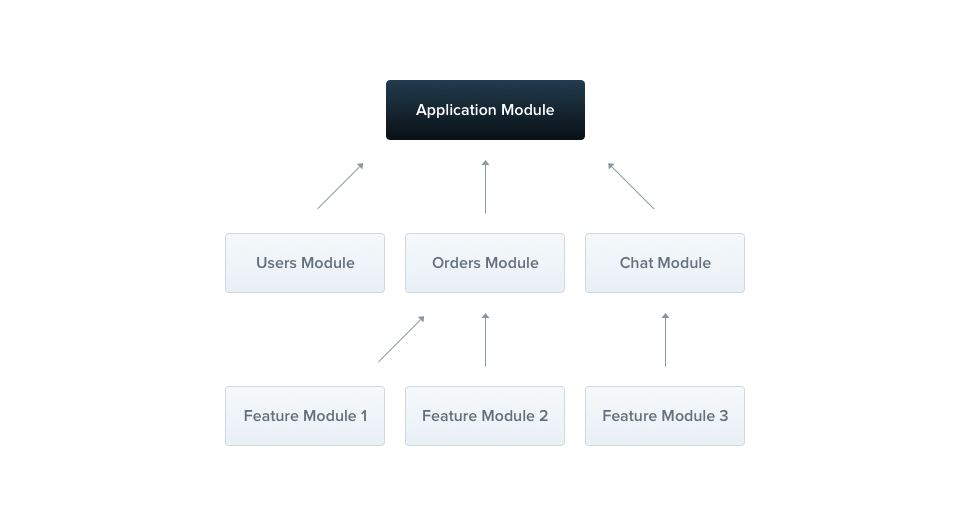
\includegraphics[width=1\textwidth]{Images/technology/module-nestjs.png}
        \caption{NestJS được tổ chức thành các đơn vị gọi là module}
    \end{figure}
Một trong những điểm quan trọng khi áp dụng NestJS vào dự án là sự xuất hiện của 3 khái niệm Modules, Controllers và Services
\begin{itemize}
    \item \textbf{Module}: Ứng dụng dựa trên nền tảng NestJS được xây dựng bằng các modules. Modules là các containers chứac các thành phần khác nhau của ứng dụng như services, controllers và các components có liên quan. Module có chức năng quản lý và đóng gói các tính năng của ứng dụng. Một module có thể là một tính năng hoặc một phần của ứng dụng. Ví dụ như có thể tồn tại các module về xác thực (authentication) , quản lý người dùng (user management), hoặc quản lý sản phẩm. Mục đích của cách tiếp cận này là dễ dàng quản lý các tính năng và đem lại sự tiện lợi trong việc nâng cấp và bảo trì ứng dụng.

    \item \textbf{Controllers}: có tác dụng xử lý các yêu cầu HTTP và đưa ra các response, phục vụ các entry point về phần logic của ứng dụng. Mỗi một controller sẽ gắn với một route cụ thể hoặc một endpoint mà ở đó được định nghĩa các function để xử lý các yêu cầu. Controllers sử dụng các decorators để tương tác với các route path bằng các phương thức HTTP bao gồm (GET, POST, PUT, DELETE,...) và các parameters. Các controller cũng có thể tương tác với service để thực hiện các business logic.
    \begin{figure}[H]
        \centering
        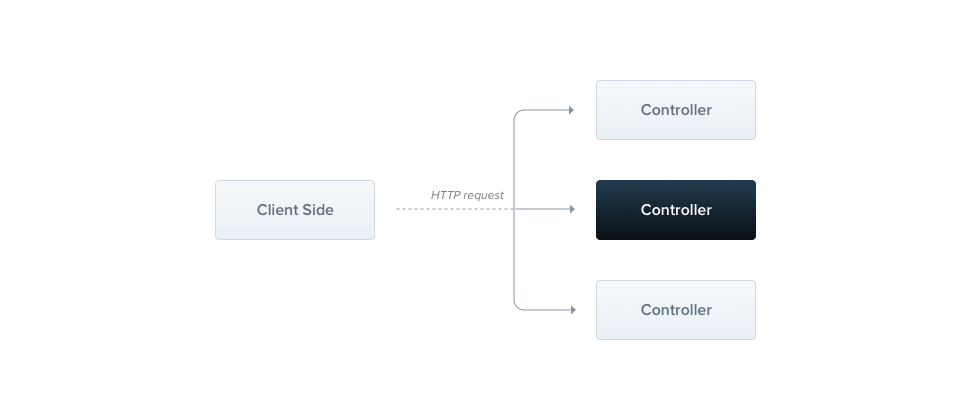
\includegraphics[width=1\textwidth]{Images/technology/controller_2.png}
        \caption{Controller của NestJS xử lý các endpoint được gọi từ phía client}
    \end{figure}
    \begin{figure}[H]
        \centering
        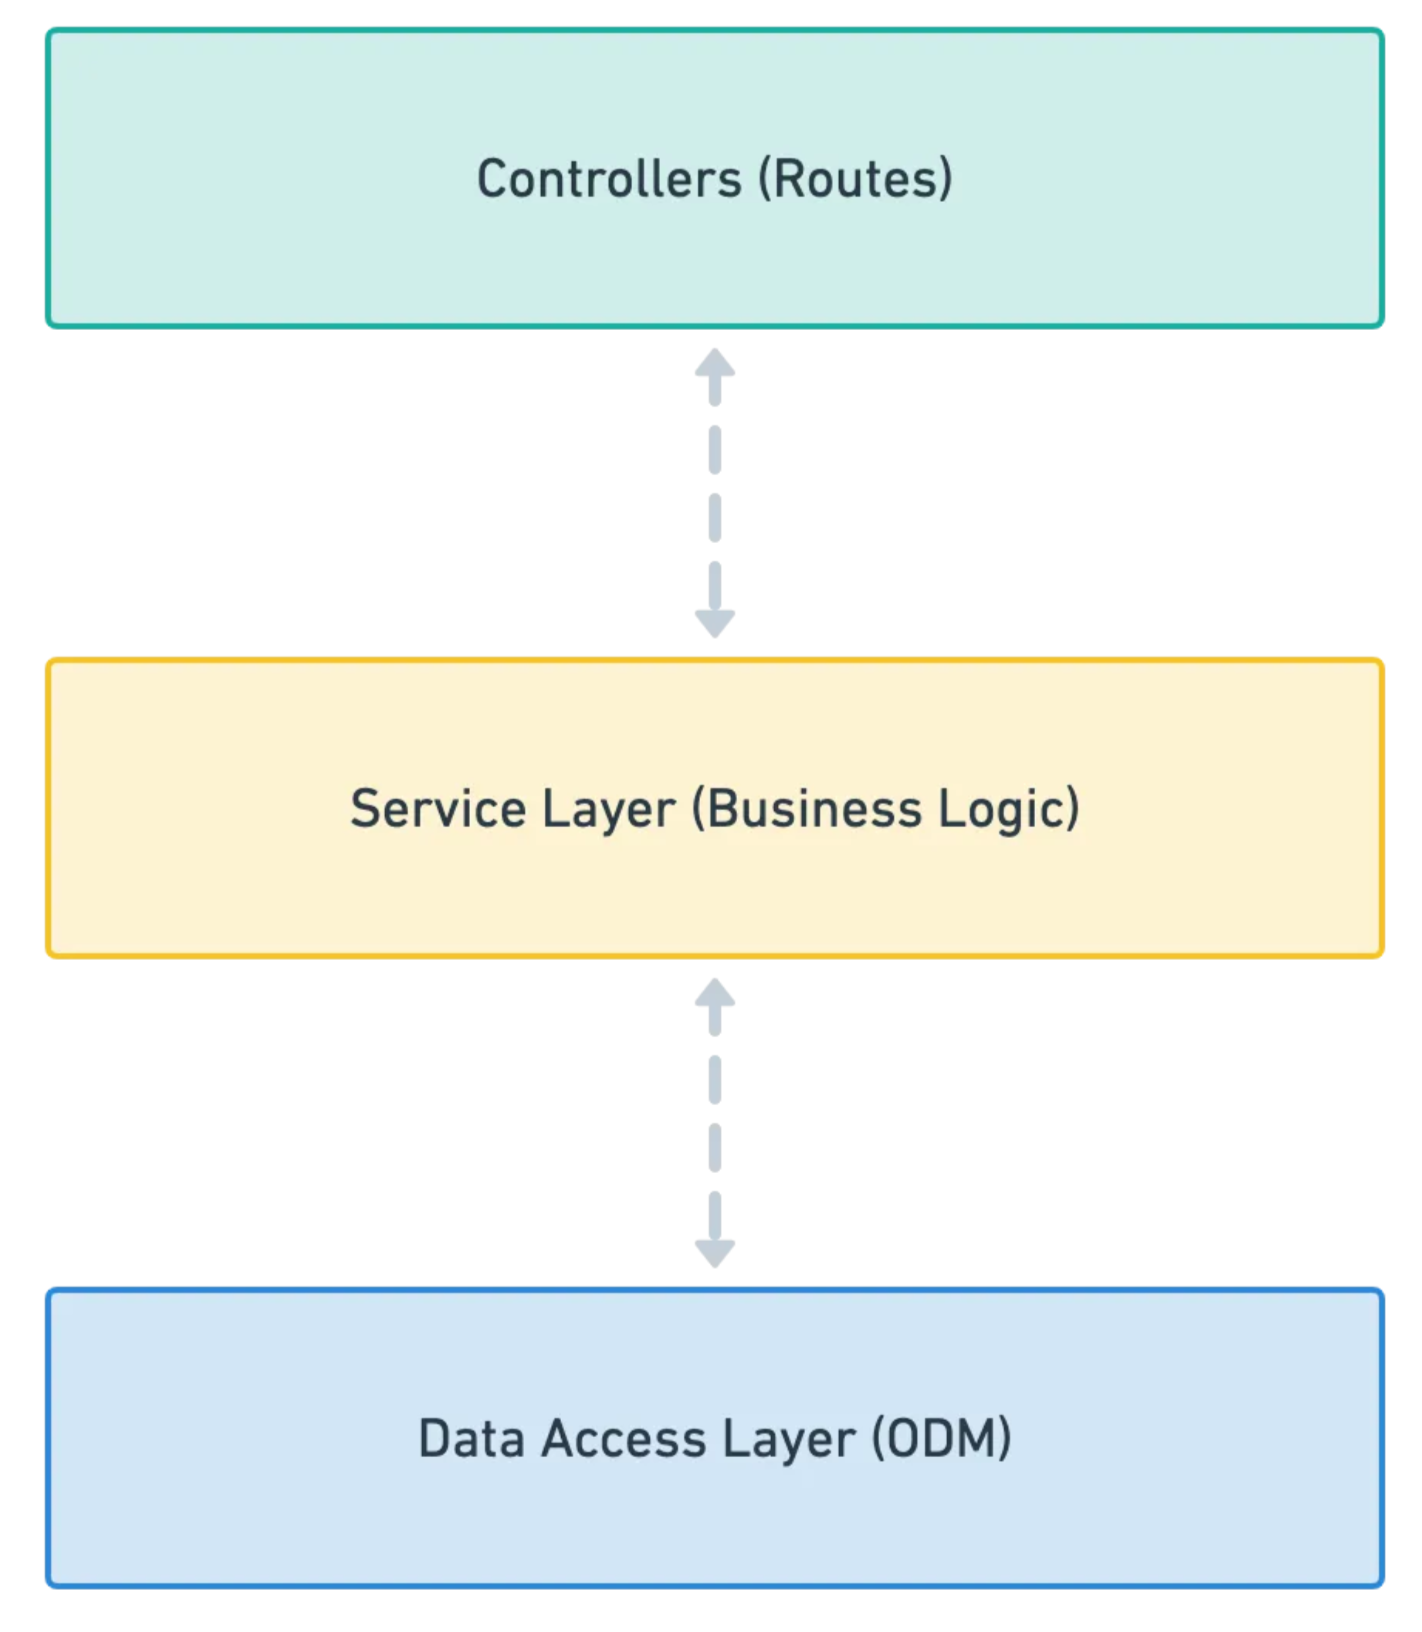
\includegraphics[width=0.4\textwidth]{Images/technology/controller.png}
        \caption{Các layer trong một ứng dụng NestJS}
    \end{figure}
    
    \item \textbf{Services}: có chức năng để định nghĩa các hàm xử lý các logic và data trong một dự án sử dụng NestJS. Service đóng gói các business logic và các hàm để xử lý data, sau đó các hàm trên sẽ được gọi trong controllers để thực hiện các chức năng như lấy dữ liệu từ database, tương tác với API hoặc xử lý các tính năng liên quan đến data. Service đóng vai trò như một chức năng của úng dụng khi mà controllers được dùng để xử lý các yêu cầu được gửi đến và đi. Service thường được sử dụng trực tiếp tại controllers mà ở NestJS được miêu tả với một từ rất đặc trưng \textbf{Injectable} tại file service để giúp dễ dàng quản lý các dependencies và nâng cao khả năng kiểm thử.
\end{itemize}
\subsubsection{Các tính năng nổi bật}
Các tính năng nổi bật của NestJS bao gồm:
\begin{itemize}
    \item Kiến trúc theo module: NestJS phát triển kiến trúc theo module để lập trình viên tiện trong việc quản lý dự án theo module, components, services và các controllers. Mục đích của việc này là nhằm tối ưu dự án để dễ nâng cấp và bảo trì
    \item Được tối ưu cho Typescript do vậy NestJS đem đến cho người dùng các lợi ích về codebase cũng như khả năng tìm ra lỗi, debug nhanh hơn
    \item Module microservices của NestJS hỗ trợ đủ loại kết nối: RabbitMQ, gRPC, Kafka, Redis,...
    \item Middleware và Guard được tích hợp trong NestJS, với vai trò để thực hiện các task như authentication, logging, hoặc data validation.
    \item Exception Handling: NestJS cung cấp một cơ chế xử lý exception dễ dàng, cho phép quản lý và xử lý các ngoại lệ trong ứng dụng.
    \item WebSocket: NestJS hỗ trợ WebSocket, cho phép xử lý kết nối realtime giữa client và server.
\end{itemize}
\subsubsection{Phân tích ưu và nhược điểm}
\textbf{Ưu điểm}
\begin{itemize}
    \item Khả năng mở rộng và bảo trì tốt do được xây dựng trên kiến trúc module, và đồng thời quản lý code được dễ dàng hơn
    \item Testing được cung cấp các dependencies để sử dụng khi viết unit test, integration test hoặc end to end test được gọn gàng hơn
    \item Tích hợp được với nhiều thư viện, kết hợp tốt với các tool và framework, ngoài ra có một số lượng lớn người sử dụng nên sẽ hiệu quả trong việc sửa lỗi khi gặp vấn đề
\end{itemize}
\textbf{Nhược điểm}
\begin{itemize}
    \item Không thích hợp với các dự án nhỏ do quá trình setup khá phức tạp, tốn rất nhiều công sức
    \item Cộng đồng chỉ đang phát triển chưa thực sự quá lớn mạnh.
    \item Kiến trúc được lấy cảm hứng từ Angular do vậy sẽ gặp khó khăn nếu như chưa từng làm qua Angular
\end{itemize}
\subsection{PostgreSQL}
\subsubsection{Tổng quan}
PostgreSQL là một hệ quản lý cơ sở dữ liệu được dùng khá phổ biến và được biết đến với nhiều tính năng tốt, khả năng mở rộng tốt cũng như cách quản lý mã nguồn hiệu quả
\subsubsection{Các tính năng nổi bật}
PostgreSQL là một trong những hệ quản trị cơ sở dữ liệu quan hệ phổ biến nhất và được sử
dụng rộng rãi trên thế giới. Nó được ưa chuộng bởi: 
\begin{itemize}
    \item PostgreSQL cung cấp khả năng bảo mật tốt, khả năng chịu đựng lỗi cao mà không ảnh hưởng đến các phần khác 
    \item Có khả năng mở rộng cao cả về số lượng dữ liệu và số lượng người dùng có thể thao tác cùng lúc
    \item Truy vấn nhanh chóng và bảo mật duy trì tính toàn vẹn và độ tin cậy. Để đáng tin cậy hơn
    \item Khả năng tương thích đa nền tảng, khả năng đồng thời xử lý nhiều kết nối, hiệu suất cao và khả năng xử lý dữ liệu lớn.
\end{itemize}
\subsubsection{Phân tích ưu và nhược điểm}
\textbf{Ưu điểm}
\begin{itemize}
    \item PostgreSQL được đánh giá là một trong những hệ quản trị cơ sở dữ liệu có độ tin tưởng cũng như bảo mật cao
    \item PostgreSQL cũng được trang bị nhiều tính năng để xử lý với một số lượng data khổng lồ
    \item Được sử dụng để chạy trang web và ứng dụng web động.
    \item Cho phép lưu lại nhật ký và hình thành cơ sở dữ liệu hỗ trợ sửa lỗi.
\end{itemize}
\textbf{Nhược điểm}
\begin{itemize}
    \item Một số extension không được hỗ trợ trên cloud do vậy phải mất thời gian đề cấu hình chỉnh sửa theo ý muốn
    \item Không hỗ trợ real-time data trong một vài trường hợp cần real-time retrieval
    \item Hiệu suất hoạt động thực tế chậm hơn so với MySQL
    \item Nhiều ứng dụng nguồn mở chỉ hỗ trợ MySQL và không hỗ trợ PostgreSQL
\end{itemize} 
\subsection{Prisma}
\subsubsection{Tổng quan}
\hspace*{1cm} Prisma là một ORM (Object-Relational Mapping) được thiết kế để làm cho việc truy cập cơ sở dữ liệu dễ dàng hơn trong các ứng dụng Node.js và TypeScript. Nó cung cấp một API dễ sử dụng để truy cập cơ sở dữ liệu mà không cần phải viết các câu lệnh SQL trực tiếp. Prisma tự động tạo ra các bảng cơ sở dữ liệu và cập nhật cấu trúc khi thay đổi mô hình dữ liệu. Prisma hỗ trợ nhiều loại cơ sở dữ liệu như PostgreSQL, MySQL và SQLite. Trong đó ORM(object relational Mapping) là một kỹ thuật giúp chuyển các đoạn mã lưu trữ dữ liệu dưới dạng OOP(Object Oriented Programming) sang relational database \cite{prisma}.\\
\begin{figure}[H]
    \centering
    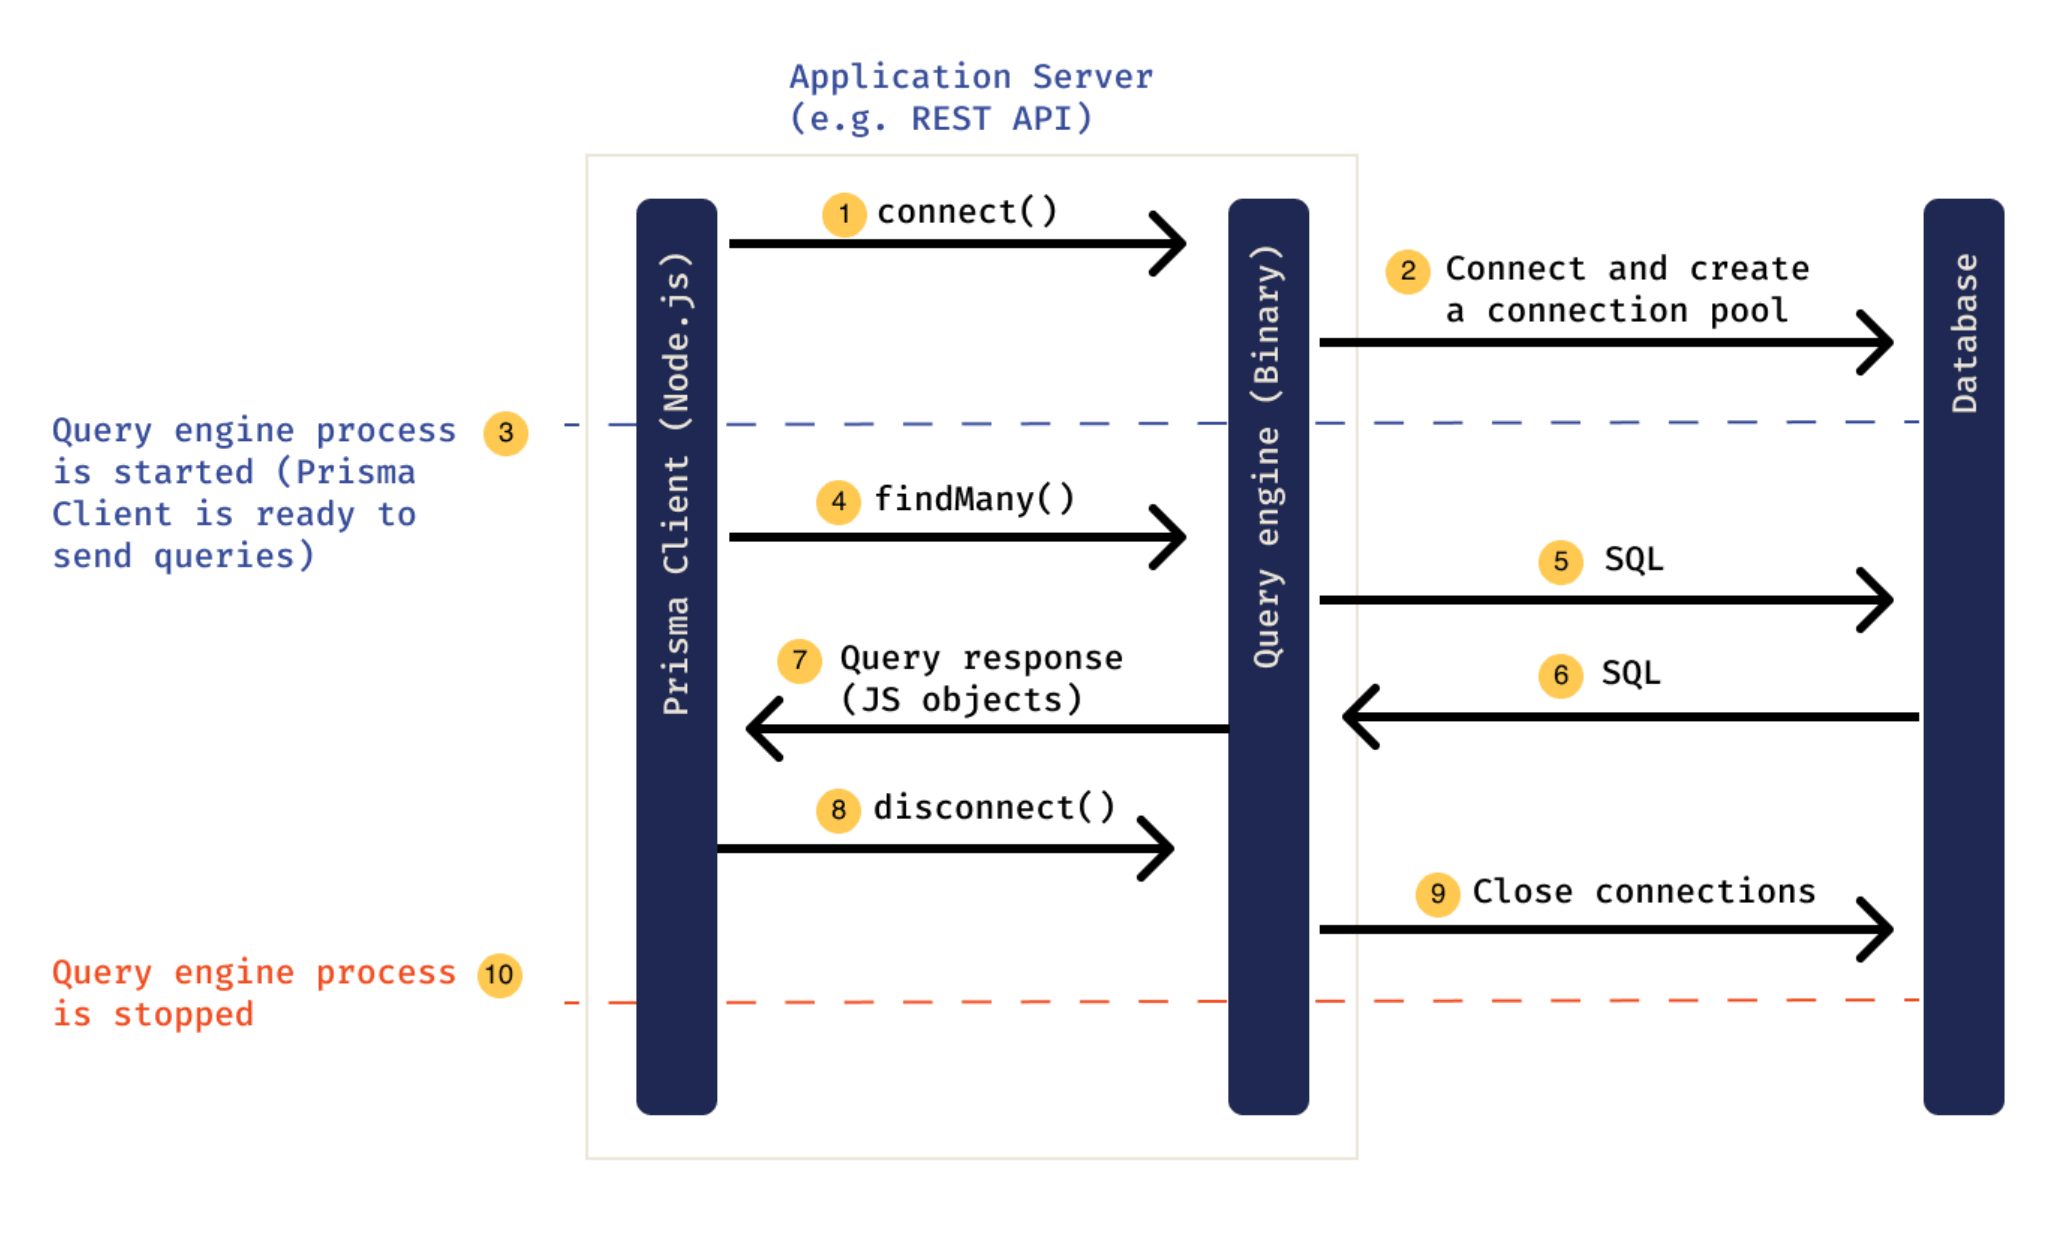
\includegraphics[width=0.9\textwidth]{Images/technology/prisma-architecture.png}
    \caption{Prisma cung cấp các phương thức để ứng dụng có thể tương tác với database}
\end{figure}
\textbf{Cách thức hoạt động của Prisma:}
\begin{enumerate}
    \item Prisma sử dụng những model được viết dưới dạng schema và lưu trữ ở client và tạo kết nối với Query Engine
    \item Tạo kết nối từ Query Engine và Database
    \item Truyền một lệnh query để truy xuất dữ liệu chuyển nó thành lệnh SQL trong Database
    \item Chờ dữ liệu gửi về từ Database
    \item Ngắt kết nối
\end{enumerate}
Prisma cung cấp một API đơn giản và dễ sử dụng để thao tác với cơ sở dữ liệu, cho phép
bạn thực hiện các thao tác CRUD (Create, Read, Update, Delete) một cách nhanh chóng và dễ
dàng.
\subsubsection{Các tính năng nổi bật}
Prisma bao gồm ba phần chính:
\begin{itemize}
    \item Prisma Client : Trình tạo truy vấn an toàn và được tạo tự động cho Node.js và TypeScript.
    \item Prisma Migrate : Hệ thống dùng để di chuyển và mô hình hóa dữ liệu.
    \item Prisma Studio : GUI để xem và chỉnh sửa dữ liệu trong cơ sở dữ liệu.
\end{itemize}
\subsubsection{Phân tích ưu và nhược điểm}
\textbf{Ưu điểm}
\begin{itemize}
    \item Prisma có khả năng mở rộng và tái sử dụng, cho phép bạn tạo ra các ứng dụng phức tạp và có thể mở rộng dễ dàng. 
    \item Prisma hỗ trợ các tính năng như transacations, batching và lazy-loading, giúp tối ưu hóa hiệu suất và giảm thiểu số lần truy cập cơ sở dữ liệu.
    \item Bên cạnh đó, Prisma cũng cho phép định nghĩa các ràng buộc duy nhất, khóa ngoại và các mối quan hệ giữa các bảng. Prisma tự động sinh ra mã TypeScript cho các truy vấn cơ sở dữ liệu, giúp bạn phát hiện lỗi trước khi thực thi chương trình.
\end{itemize}
\textbf{Nhược điểm}
\begin{itemize}
    \item Cộng đồng còn nhỏ, sẽ gặp khó khăn khi gặp vấn đề do không có nhiều người hỗ trợ
    \item Tuy Prisma cung cấp một lớp trừu tượng nhằm tăng hiệu suất và các lệnh để tương tác với database, nhưng một vài dự án đòi hỏi những lệnh query phức tạp thì chưa thể đáp ứng
\end{itemize}
\subsection{JWT}
\subsubsection{Tổng quan}
JSON Web Token (JWT) \cite{jwt} là một tiêu chuẩn mở định nghĩa một cách ngắn gọn và khép
kín để truyền dẫn thông tin giữa hai bên client và server được định dạng bằng JSON.
Chuỗi JWT gồm 3 thành phần là header, payload, signature và được ngăn cách nhau bằng
dấu chấm (“.”).
\begin{figure}[H]
    \centering
    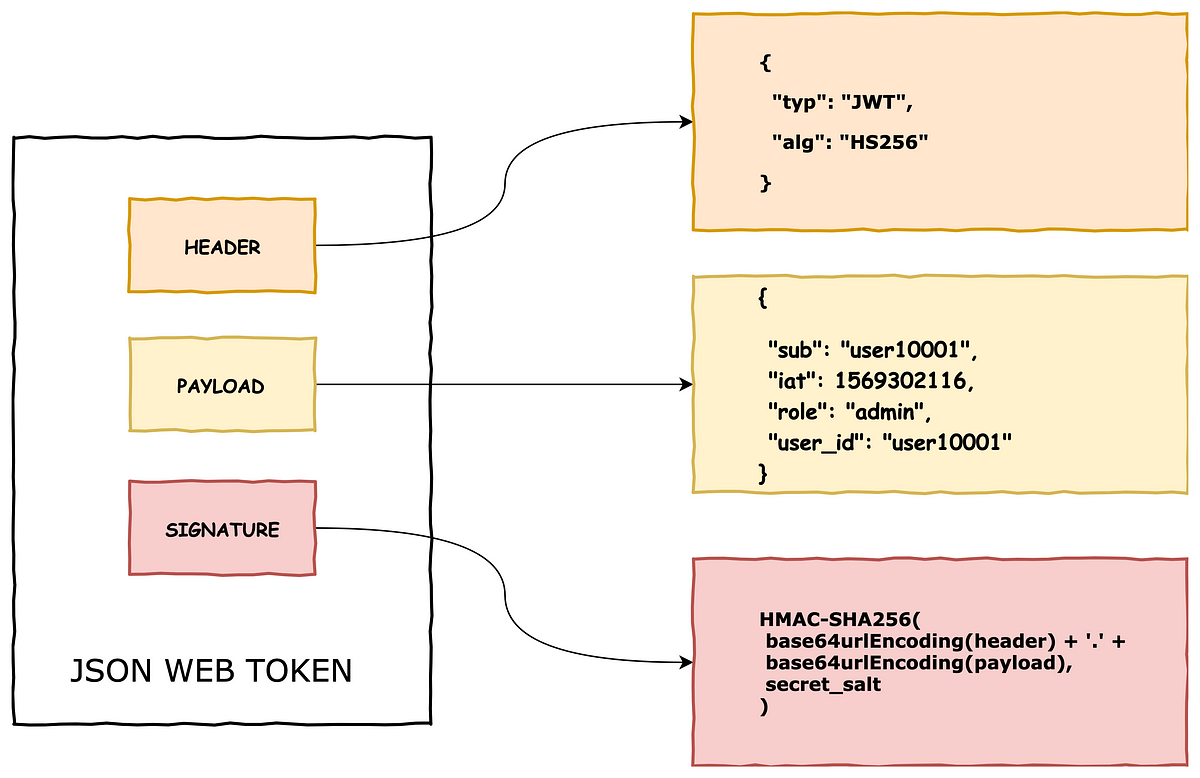
\includegraphics[width=0.7\textwidth]{Images/technology/jwt_structure.png}
    \caption{Cấu trúc của JSON web token}
\end{figure}
\begin{itemize}
    \item \textbf{Header}: Phần header thường chứa hai phần là kiểu dữ liệu (giá trị thường là JWT) và thuật toán sử dụng để mã hóa chuỗi như HMAC SHA256 hoặc RSA
    \item \textbf{Payload}: Phần payload chứa thông tin muốn đặt trong chuỗi ví dụ như tên đăng nhập (username), id của người dùng (user id), tên người dùng,...Phần payload sẽ được mã hóa Base64Url tạo thành phần thứ hai của chuỗi JWT.
    \item \textbf{Signature}: Phần signature này sẽ được tạo ra bằng cách mã hóa phần header và phần payload kèm theo một chuỗi secret (khóa bí mật)
\end{itemize}
\textbf{Quy trình của xác thực client với JWT}:
\begin{enumerate}
    \item Người dùng sẽ gửi thống tin xác thực của mình đến server xác thực.
    \item Server sẽ kiểm tra thông tin người dùng cung cấp có đúng không. Nếu dúng thì chuyển sang bước tiếp theo, ngược lại thì trả lỗi về cho người dùng.
    \item Server xác thực sẽ thực hiện ký lên thông tin của người dùng kèm với một số claims khác như thời gian cấp, thời điểm hết hạn và thời điểm mà token bắt đầu trở nên hợp lệ.
    \item Sau khi người dùng nhận được token, họ sẽ đính kèm token này vào các lời gọi API (thường là bỏ ở header Authorization của api request).
    \item Server xử lý các api request sẽ tiến hành parse token và xử lý xác thực để cho phép người dùng truy cập các resource
\end{enumerate}
\begin{figure}[H]
    \centering
    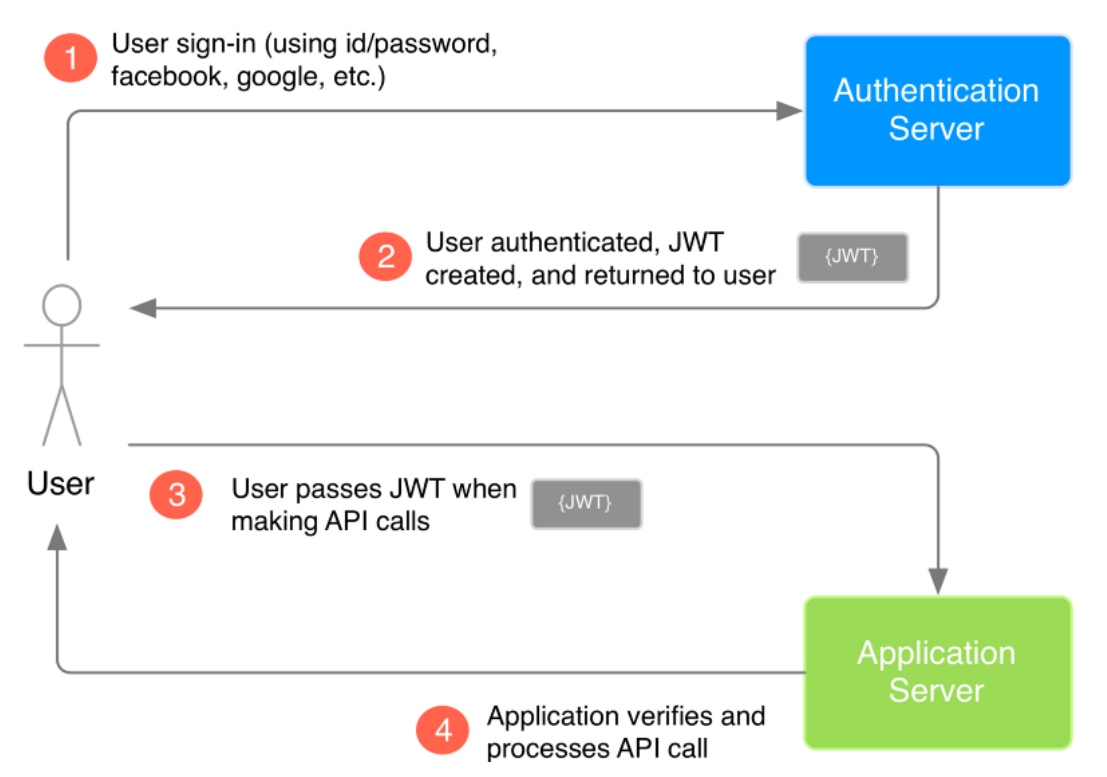
\includegraphics[width=0.7\textwidth]{Images/technology/jwt authentication.png}
    \caption{Quy trình xác thực client với JWT}
\end{figure}
\subsubsection{Các tính năng nổi bật}
\begin{itemize}
    \item \textbf{Xác thực (Authentication)}: Đây là trường hợp phổ biến nhất sử dụng JWT. Sau khi người dùng đăng nhập vào hệ thống, thì những request tiếp theo từ phía người dùng sẽ chứa thêm mã JWT. Điều này cho phép người dùng có quyền truy cập vào các url, service, và resource mà mã Token đó cho phép.
    \item \textbf{Trao đổi thông tin}: JWT là 1 cách khá hay để truyền thông tin an toàn giữa các thành viên với nhau. Và nhờ vào phần signature của nó, phía người nhận có thể biết được người gửi là ai thông qua phần signature. Và chữ ký được tạo ra bằng việc kết hợp cả phần header và phần payload lại nên thông qua đó ta có thể xác nhận được chữ ký đó có bị giả mạo hay không.
\end{itemize}

\subsubsection{Phân tích ưu và nhược điểm}
\textbf{Ưu điểm}
\begin{itemize}
    \item Đơn giản, gọn nhẹ: Như ta có thể thấy ở trên, việc xác thực với JWT vô cùng đơn giản và gọn nhẹ. Việc lưu trữ token hoàn toàn nằm ở phía client giúp phần nào giảm tải được nhu cầu về tài nguyên lưu trữ và tính toán ở server. Đây là một ưu điểm nổi bật khi so sánh với các phương pháp truyền thống khác sử dụng Session hay Cookies.
    \item Dễ lập trình: JWT được hỗ trợ và sử dụng rộng rãi nên hầu như tất cả ngôn ngữ lập trình backend đều hỗ trợ việc tạo và xác thực các JWT một cách tiện lợi.
    \item Dễ scale: việc xác thực với JWT không yêu cầu lưu trữ thêm thông tin ở phía server, ứng dụng của ta có thể scale tốt hơn mà không phải tốn thêm quá nhiều chi phí cho các server và database xác thực người dùng.
\end{itemize}
\textbf{Nhược điểm}
\begin{itemize}
    \item  Vì JWT token nằm hoàn toàn ở phía client nên ta không thể hủy các token một cách chủ động từ backend. Để chống một số loại tấn công DOS ta phải ràng buộc thời hạn hợp lệ của token và hiện thực thêm các cơ chế cấp lại token mới cho người dùng.
\end{itemize}
\chapter{HIỆN THỰC GIẢI PHÁP}
\section{CẤU TRÚC MÃ NGUỒN}
\subsection{Cấu trúc mã nguồn front-end}
Trên đây là cấu trúc mã nguồn của phần frontend trong dự án, trong dự án này, cả nhóm sử dụng công nghệ expo go để hiện thực ứng dụng, tại đây sẽ có các thư mục quan trọng như sau:
\begin{itemize}
    \item \textit{app:} chứa source code chính của dự án, như chúng ta có thể quan sát được, những folder được đặt tên trong cặp dấu ( ) như (tabs) hoặc (auth) là định dạng được expo go quy định để áp dụng stack screen và tab screen cho màn hình ứng dụng, \_layout sẽ chứa các màn hình được áp dụng stack screen và tab screen
    \item \textit{asset:} chứa các tài nguyên như hình ảnh, font chữ, các file text,...
    \item \textit{components:} chứa các components được dùng đi dùng lại nhiều lần trong thời gian phát triển app
    \item \textit{server:} chứa các hàm để gọi api push, post, patch, get cho các chức năng trong app như authentication, lấy danh sách nhà, tìm danh sách nhà dựa trên từ khóa,...
    \item \textit{\_layout.tsx:} đây là file để lưu trữ Tab layout có tác dụng cấu trúc tab navigation cho ứng dụng, di chuyển giữa các tab với nhau
    \item \textit{patches:} sử dụng patches để chỉnh sửa các file thư viện trong node modules sao cho trùng khớp với version của nhau để ứng dụng có thể chạy mà không bị gặp lỗi
    \item \textit{eas-json:} cấu hình app để xây dựng ứng dụng dưới dạng file .apk hoặc là link qr code để quét sử dụng
    \item \textit{Thư mục dist:} Thư mục này là kết quả thực thi câu lệnh \textit{npm run build} để tạo ra dự án sản phẩm hoàn thiện có thể sẵn sàng được triển khai trên các nền tảng để sử dụng.
    \item \textit{Thư mục node\_modules:} Thư mục này chứa các gói cài đặt thư viện của bên thứ ba cần thiết để phục vụ cho việc xây dựng các chức năng khác nhau của ứng dụng.
    \item \textit{package-lock.json:} \textit{File} này là một phần quan trọng của dự án \textit{Node.js} sử dụng \textit{npm}. Nó tự động được tạo và cập nhật bởi \textit{npm} khi cài đặt các gói phụ thuộc. \textit{File} này ghi lại chính xác phiên bản của từng gói đã được cài đặt trong dự án, bao gồm các gói phụ thuộc của chúng. Điều này đảm bảo rằng các cài đặt trong tương lai sẽ sử dụng cùng một phiên bản gói, giúp tránh các vấn đề về tương thích và lỗi do thay đổi phiên bản. \textit{File} \textit{package-lock.json} giúp duy trì sự nhất quán và ổn định cho dự án khi làm việc trên nhiều môi trường hoặc khi cộng tác với các nhà phát triển khác.
    \item \textit{package.json:} \textit{File} này chứa thông tin về dự án và các gói phụ thuộc. \textit{File} này định nghĩa các thông tin cơ bản như tên dự án (\textit{name}), phiên bản (\textit{version}), và các \textit{scripts} để thực hiện các tác vụ như xây dựng (\textit{build}), kiểm tra (\textit{test}), và khởi động (\textit{start}) ứng dụng. Các gói phụ thuộc chính (\textit{dependencies}) và phụ thuộc phát triển (\textit{devDependencies}) được liệt kê để quản lý phiên bản và cài đặt. Cấu hình cho \textit{jest} cũng được bao gồm để thiết lập môi trường kiểm thử. \textit{File} này giúp quản lý các công cụ và thư viện cần thiết cho dự án, đảm bảo rằng mọi thành viên trong nhóm sử dụng cùng một phiên bản gói và cấu hình.
\end{itemize}
\subsection{Cấu trúc mã nguồn back-end}
Cấu trúc mã nguồn của \textit{back-end} bao gồm các thư mục và các \textit{file} được mô tả như sau:
\begin{itemize}
    \item \textit{Thư mục dist:} Thư mục này là kết quả thực thi câu lệnh \textit{npm run build} để tạo ra dự án sản phẩm hoàn thiện có thể sẵn sàng được triển khai trên các nền tảng để sử dụng.
    \item \textit{Thư mục node\_modules:} Thư mục này chứa các gói cài đặt thư viện của bên thứ ba cần thiết để phục vụ cho việc xây dựng các chức năng khác nhau của ứng dụng.
    \item \textit{Thư mục prisma:} Thư mục này chứa \textit{file schema.prisma} để ánh xạ cơ sở dữ liệu với cú pháp do \textit{Prisma ORM} định nghĩa để chuyển đổi qua cơ sở dữ liệu thực sự ở \textit{PostgreSQL}. Ngoài ra thư mục này còn chứa \textit{API} để \textit{back-end} có thể làm việc được với cơ sở dữ liệu \textit{PostgreSQL} thông qua lớp trung gian do \textit{Prisma ORM} cung cấp, các \textit{API} này được lưu trữ trong thư mục \textit{client}.
    \item \textit{Thư mục src/domains:} Thư mục này là nơi để hiện thực toàn bộ các chức năng chính cho ứng dụng. Trong đó mỗi chức năng sẽ được tổ chức thành một thư mục riêng, và trong mỗi thư mục sẽ chứa các thư mục \textit{request} và \textit{response} để định nghĩa kiểu cho các yêu cầu \textit{request} và phản hồi \textit{response}. Cùng với đó là các \textit{file <name>.module.ts} để đóng gói các thành phần bên trong thành một chức năng hoàn chỉnh, \textit{file} này quy định về các \textit{controller} và \textit{service} được sử dụng cho chức năng đó, ngoài ra có thể \textit{import} từ \textit{module} khác hoặc xuất ra \textit{service} để \textit{module khác có thể sử dụng}. File \textit{<name>.controller.ts} được dùng để định nghĩa các \textit{endpoint} cho chức năng đó, bao gồm kiểu \textit{HTTP request}, kiểu \textit{request} và \textit{response}, với mỗi \textit{endpoint}, \textit{controller} sẽ gọi tới \textit{method} trong \textit{service} tương ứng. Cuối cùng là \textit{file} \textit{<name>.service.ts}, đây là nơi hiện thực \textit{business logic} dành cho chức năng đó, bao gồm việc xử lý \textit{database}, gọi tới \textit{service} của bên thứ ba...
    \item \textit{Thư mục src/interceptors:} Thư mục này chứa \textit{file logger.interceptor.ts} để ghi lại các thông tin quan trọng về \textit{request} như đường dẫn \textit{endpoint} và phương thức \textit{HTTP}, hỗ trợ trong quá trình \textit{debug} và giám sát ứng dụng bằng cách cung cấp những thông tin chi tiết về các \textit{request} đang được gửi đến. Điều này giúp cho việc phát hiện và sửa lỗi nhanh chóng hơn, đồng thời cũng cung cấp một cách thức để theo dõi hoạt động của hệ thống một cách hiệu quả. \textit{Interceptor} là một phần quan trọng trong việc quản lý và duy trì tính ổn định của ứng dụng \textit{NestJS}.
    \item \textit{Thư mục src/middlewares:} Thư mục này chứa \textit{file error.middleware.ts} để cung cấp một bộ lọc ngoại lệ \textit{(Exception Filter)} quan trọng, giúp ứng dụng xử lý các ngoại lệ và lỗi một cách trực quan. Nó bắt và ghi \textit{log} các ngoại lệ, xác định \textit{status code} phản hồi dựa trên loại ngoại lệ, và cung cấp các thông tin chi tiết như tên, thông điệp lỗi, đường dẫn \textit{request}, và thời gian xảy ra lỗi. Điều này giúp cải thiện quản lý lỗi và dễ dàng theo dõi, giám sát hiệu quả hoạt động của ứng dụng.
    \item \textit{Thư mục src/validation:} Thư mục này chứa \textit{file pipe.validation.ts}  dùng để xử lý và kiểm tra dữ liệu đầu vào. \textit{ValidationPipe} chuyển đổi dữ liệu thành đối tượng dựa trên \textit{metadata} và kiểm tra tính hợp lệ bằng \textit{class-validator}, xử lý lỗi bằng cách ném ra \textit{HttpException} nếu có lỗi. \textit{ParseArrayPipe} biến đổi một mảng giá trị thành mảng các đối tượng, áp dụng kiểm tra tính hợp lệ và ném ra \textit{HttpException} nếu có lỗi. Cả hai loại \textit{pipe} trên đều giúp bảo vệ và xử lý dữ liệu một cách an toàn trước khi chúng được truyền vào các phương thức xử lý chính của ứng dụng \textit{NestJS}.
    \item \textit{Thư mục src/services:} Thư mục này cung cấp các dịch vụ ở bên thứ ba để hỗ trợ cho các chức năng của ứng dụng, bao gồm dịch vụ kết nối với cơ sở dữ liệu, kết nối với dịch vụ đám mây \textit{Cloudinary}, kết nối với mô hình ngữ nghĩa sinh \textit{vector} từ văn bản.
    \item \textit{Thư mục src/utils:} Thư mục này chứa các kiểu lớp dùng chung cho toàn bộ ứng dụng, ví dụ như kiểu \textit{request} dùng cho cho các \textit{API} liên quan đến lấy danh sách, chức năng phân trang, kiểu trả về đối với các phương thức \textit{void}...
    \item \textit{.env:} \textit{File} này chứa các biến môi trường được sử dụng để cấu hình ứng dụng \textit{NestJS}. Các biến bao gồm địa chỉ \textit{URL} kết nối đến cơ sở dữ liệu \textit{PostgreSQL}, cùng với các thông tin nhạy cảm như khóa bí mật \textit{JWT} và thông tin xác thực của dịch vụ \textit{Cloudinary}. Các biến này đảm bảo ứng dụng có thể kết nối và sử dụng các dịch vụ bên ngoài một cách an toàn và hiệu quả. Ngoài ra, còn có biến để cấu hình thời gian hết hạn của \textit{token} truy cập \textit{JWT} và các \textit{URL} khác để tích hợp với các dịch vụ ngoài.
    \item \textit{.eslintrc.js}: \textit{File} này là cấu hình cho \textit{ESLint}, một công cụ phân tích tĩnh mã nguồn để tìm lỗi trong \textit{code}. Cấu hình này được thiết lập để làm việc với \textit{TypeScript} và \textit{Prettier} nhằm đảm bảo mã nguồn tuân theo các quy tắc nhất định và được định dạng nhất quán. Cụ thể, nó sử dụng parser \textit{@typescript-eslint/parser}, các plugin như \textit{@typescript-eslint/eslint-plugin}, và mở rộng các cấu hình đề xuất từ \textit{plugin:@typescript-eslint/recommended} và \textit{plugin/recommended}. Ngoài ra, nó định nghĩa môi trường là \textit{node} và \textit{jest}, và thiết lập một số quy tắc cụ thể để kiểm soát cách \textit{code} được viết và định dạng.
    \item \textit{.gitignore:} Đượcdùng để loại trừ các \textit{file} và thư mục không cần thiết khỏi hệ thống kiểm soát phiên bản \textit{Git}. \textit{File} này bao gồm các thư mục biên dịch như \textit{/dist}, \textit{/node\_modules}, và \textit{/prisma}, cũng như các \textit{file} cấu hình môi trường như \textit{.env}. Nó cũng loại trừ các \textit{file} nhật ký (\textit{logs}, \textit{*.log}) và các thư mục đầu ra kiểm thử (\textit{/coverage}, \textit{/.nyc\_output}). Ngoài ra, \textit{file} này còn loại trừ các \textit{file} và thư mục cấu hình của các IDE và trình soạn thảo, bao gồm \textit{VSCode}, \textit{.idea}, và \textit{.vscode}.
    \item \textit{.pretierrc:} Được sử dụng để định dạng mã nguồn tự động theo các quy tắc đã chỉ định. \textit{File} này thiết lập các quy tắc định dạng như sử dụng dấu nháy đơn (\textit{singleQuote}: \textit{true}), thêm dấu phẩy cuối cùng (\textit{trailingComma}: \textit{all}), độ rộng tab là 4 ký tự (\textit{tabWidth}: 4), không sử dụng tab (\textit{useTabs}: \textit{false}), kết thúc dòng tự động (\textit{endOfLine}: \textit{auto}), sử dụng dấu chấm phẩy (\textit{semi}: \textit{true}), và độ rộng dòng tối đa là 130 ký tự (\textit{printWidth}: 130). Những thiết lập này giúp đảm bảo mã nguồn được định dạng nhất quán trong toàn bộ dự án.
    \item \textit{nest-cli.json:} \textit{File} này thiết lập các thông số cho \textit{Nest CLI}, bao gồm URL \textit{schema} để xác thực cấu hình, bộ sưu tập mặc định là \textit{@nestjs/schematics}, và thư mục nguồn là \textit{src}. Ngoài ra, nó còn chứa tùy chọn biên dịch (\textit{compilerOptions}) để tự động xóa thư mục đầu ra (\textit{deleteOutDir}: \textit{true}) trước khi biên dịch lại. Cấu hình này giúp duy trì tổ chức và nhất quán trong quy trình phát triển ứng dụng \textit{NestJS}.
    \item \textit{package-lock.json:} \textit{File} này là một phần quan trọng của dự án \textit{Node.js} sử dụng \textit{npm}. Nó tự động được tạo và cập nhật bởi \textit{npm} khi cài đặt các gói phụ thuộc. \textit{File} này ghi lại chính xác phiên bản của từng gói đã được cài đặt trong dự án, bao gồm các gói phụ thuộc của chúng. Điều này đảm bảo rằng các cài đặt trong tương lai sẽ sử dụng cùng một phiên bản gói, giúp tránh các vấn đề về tương thích và lỗi do thay đổi phiên bản. \textit{File} \textit{package-lock.json} giúp duy trì sự nhất quán và ổn định cho dự án khi làm việc trên nhiều môi trường hoặc khi cộng tác với các nhà phát triển khác.
    \item \textit{package.json:} \textit{File} này chứa thông tin về dự án và các gói phụ thuộc. \textit{File} này định nghĩa các thông tin cơ bản như tên dự án (\textit{name}), phiên bản (\textit{version}), và các \textit{scripts} để thực hiện các tác vụ như xây dựng (\textit{build}), kiểm tra (\textit{test}), và khởi động (\textit{start}) ứng dụng. Các gói phụ thuộc chính (\textit{dependencies}) và phụ thuộc phát triển (\textit{devDependencies}) được liệt kê để quản lý phiên bản và cài đặt. Cấu hình cho \textit{jest} cũng được bao gồm để thiết lập môi trường kiểm thử. \textit{File} này giúp quản lý các công cụ và thư viện cần thiết cho dự án, đảm bảo rằng mọi thành viên trong nhóm sử dụng cùng một phiên bản gói và cấu hình.
    \item \textit{tsconfig.build.json:} \textit{File} này mở rộng từ cấu hình cơ bản đã được định nghĩa trong \textit{file} \textit{tsconfig.json} (\textit{extends: "./tsconfig.json"}), nghĩa là nó sử dụng các thiết lập đã được định nghĩa trong đó. Đồng thời, nó xác định các thư mục và \textit{file} sẽ bị loại bỏ khỏi quá trình biên dịch (\textit{exclude}). Cụ thể, các thư mục \textit{node\_modules}, \textit{test}, và \textit{dist} sẽ không được bao gồm trong quá trình biên dịch, và tất cả các \textit{file} có tên kết thúc bằng \textit{spec.ts} cũng sẽ được loại bỏ. Cấu hình này giúp đảm bảo rằng \textit{TypeScript} chỉ biên dịch các \textit{file} cần thiết và loại bỏ các \textit{file} không cần thiết trong quá trình phát triển và xây dựng dự án.
    \item \textit{tsconfig.json:} \textit{File} này xác định các tùy chọn biên dịch như \textit{module commonjs}, hỗ trợ \textit{decorator} và \textit{import} mặc định tổng hợp. Nó sử dụng phiên bản \textit{target} là \textit{ES2021} và tạo các \textit{file} bản đồ nguồn để hỗ trợ gỡ lỗi. \textit{File} cũng chỉ định thư mục đầu ra là \textit{./dist} và kích hoạt biên dịch tăng dần để cải thiện hiệu suất. Cấu hình này giúp trong quá trình phát triển và triển khai ứng dụng \textit{TypeScript}, đảm bảo tính nhất quán và hiệu suất trong biên dịch mã nguồn.
    \item \textit{vercel.json:} \textit{File} này được sử dụng để triển khai ứng dụng trên nền tảng \textit{Vercel}. \textit{File} này định nghĩa phiên bản cấu hình là 2 (\textit{"version": 2}), và có hai phần chính là \textit{"builds"} và \textit{"routes"}. Phần \textit{"builds"} chỉ định nguồn của mã nguồn là tệp src/main.ts và sử dụng \textit{module @vercel/node} để xây dựng. Phần \textit{"routes"} quản lý các tuyến đường của ứng dụng, mỗi yêu cầu (bao gồm \textit{GET, POST, PUT, PATCH, DELETE, OPTIONS}) sẽ được định tuyến đến \textit{file src/main.ts}, với cài đặt \textit{header} cho phép \textit{CORS("Access-Control-Allow-Origin: *"}). Cấu hình này giúp đảm bảo ứng dụng của hoạt động mượt mà và có tính linh hoạt trong việc xử lý các yêu cầu khác nhau trên nền tảng \textit{Vercel}.
\end{itemize}
\subsection{Cấu trúc mã nguồn mô hình tìm kiếm hybrid}
\hspace*{1cm}
Cấu trúc mã nguồn của mô hình tìm kiếm \textit{hybrid} bao gồm các thư mục và các \textit{file} được mô tả như sau:
\begin{itemize}
    \item \textit{Thư mục pycache:} Đây là thư mục tự động được \textit{Python} tạo ra để lưu trữ các \textit{file} tin \textit{bytecode} đã được biên dịch (có đuôi \textit{.pyc}). Những \textit{file} này giúp tăng tốc độ khởi động ứng dụng khi chạy lại mã nguồn.
    \item \textit{Thư mục .venv:} Đây là thư mục chứa môi trường ảo của \textit{Python}. Môi trường ảo cho phép tạo một môi trường độc lập để quản lý các gói thư viện mà không ảnh hưởng đến hệ thống \textit{Python} toàn cục. Điều này đặc biệt hữu ích khi cần các phiên bản khác nhau của các gói thư viện cho các dự án khác nhau.
    \item \textit{Thư mục static:} Đây là thư mục thường dùng để lưu trữ các tài nguyên tĩnh như hình ảnh, \textit{file} \textit{CSS}, \textit{file} \textit{JavaScript}, và các tài nguyên khác mà trình duyệt có thể tải trực tiếp mà không cần xử lý từ phía máy chủ. Trong thư mục này có \textit{file} \textit{style.css}, là \textit{file} định kiểu \textit{CSS} để tạo giao diện cho trang \textit{web}.
    \item \textit{Thư mục templates:} Thư mục này chứa các \textit{file} \textit{HTML} dùng làm mẫu để tạo ra các trang \textit{web} động. Thông thường, các \textit{file} \textit{HTML} trong thư mục này sẽ chứa các \textit{placeholder} để được thay thế bằng dữ liệu thực tế từ máy chủ khi trang \textit{web} được tải. Trong thư mục này có \textit{file} \textit{index.html}, là trang chính của ứng dụng \textit{web}.
    \item \textit{\textit{File} .env:} Đây là \textit{file} môi trường \textit{(environment file)} dùng để lưu trữ các biến môi trường như các khóa \textit{API}, thông tin cấu hình cơ sở dữ liệu, và các thông tin bí mật khác. Các biến môi trường này sẽ được đọc vào khi ứng dụng khởi động. Trong\textit{file} này, nhóm định nghĩa kết nối \textit{database} để có thể kết nối từ ứng dụng.
    \item \textit{\textit{File} .gitignore:} \textit{File} này chứa danh sách các \textit{file} và thư mục cần được bỏ qua khi sử dụng \textit{Git} để quản lý phiên bản mã nguồn. Ví dụ: các \textit{file} trong thư mục \textit{\_\_pycache\_\_}, các \textit{file} môi trường \textit{.env}, và thư mục \textit{.venv} thường được liệt kê trong \textit{.gitignore} để không bị theo dõi bởi \textit{Git}.
    \item \textit{app.py:} \textit{File} \textit{app.py} trong dự án này là \textit{file} chính của ứng dụng \textit{web}, được xây dựng bằng \textit{Flask}. Nó định nghĩa ba tuyến đường chính: 
    \begin{itemize}
        \item \textit{/embedding:} Nhận yêu cầu \textit{GET} với dữ liệu văn bản \textit{JSON}, tạo \textit{embedding} từ văn bản và trả về \textit{vector} dưới dạng array và được bọc bởi \textit{JSON}.
        \item \textit{/search:} Nhận yêu cầu \textit{GET} với truy vấn tìm kiếm \textit{JSON}, thực hiện tìm kiếm kết hợp và trả về kết quả dưới dạng \textit{JSON}.
        \item \textit{/}: Hiển thị trang chủ, \textit{render} từ \textit{file} \textit{index.html}.
    \end{itemize}
    Ngoài ra, \textit{file} này còn mở một đường hầm \textit{ngrok} để truy cập ứng dụng từ bên ngoài mạng nội bộ.
    \item \textit{combine\_listing\_information.py:} \textit{File} \textit{combine\_listing\_information.py} chứa một hàm duy nhất là \textit{combine\_listing\_information}. Hàm này nhận vào một danh sách thông tin về nhà thuê và kết hợp các thông tin này thành một chuỗi mô tả đầy đủ. Chuỗi mô tả bao gồm tên nhà thuê, giá thuê, loại, diện tích, số phòng ngủ, số nhà vệ sinh, địa chỉ, mô tả chi tiết, các tiện ích, và đánh giá trung bình. Hàm này giúp tổng hợp và định dạng thông tin nhà thuê thành một văn bản liền mạch duy nhất để sử dụng trong mô hình tìm kiếm ngữ nghĩa.
    \item \textit{embedding.py:} \textit{File} này định nghĩa hàm \textit{model\_generate\_embedding}, sử dụng mô hình \textit{BGEM3FlagModel} để tạo \textit{embedding} từ văn bản. Hàm này nhận vào một chuỗi văn bản và sử dụng mô hình để mã hóa văn bản thành các \textit{vector} nhúng, trả về kết quả dưới dạng một mảng \textit{NumPy}.
    \item \textit{hybrid\_search.py:} \textit{File} này định nghĩa các hàm tìm kiếm cho ứng dụng, bao gồm tìm kiếm toàn văn bản \textit{(FTSearch)}, tìm kiếm ngữ nghĩa \textit{(semantic search)}, và tìm kiếm kết hợp \textit{(hybrid search)}. Các hàm này sử dụng mô hình nhúng văn bản \textit{(embedding)} và mô hình \textit{CrossEncoder} để mã hóa và xếp hạng các kết quả tìm kiếm, đồng thời kết nối với cơ sở dữ liệu \textit{PostgreSQL} để truy xuất thông tin về danh sách nhà trọ.
    \item \textit{requirements.txt:} \textit{File} này liệt kê các gói thư viện \textit{Python} cần thiết cho dự án và phiên bản tương ứng của chúng
\end{itemize}
\section{XÂY DỰNG API}
\subsection{API cho các chức năng của Authentication}
\subsubsection{Sign up}
\begin{center}
    \begin{longtblr}[caption={Sign up}]{
        rows = {bg = green!10!white},
        vlines = {dashed, green!75!black},
        hlines = {dashed, green!75!black},
        hline{1-6,8} = {2pt, green!75!black},
        vline{odd} = {2pt, green!75!black},
        vline{even} = {5}{green!75!black},
        cell{1-3}{1} = {c = 4}{halign = l},
        cell{4}{1,3} = {c = 2}{halign = c},
        row{5} = {halign = c},
        cell{7}{3-4} = {bg = green!75!black}
    }
    \textit{Tên API:} \textbf{Sign up}&&&\\
    \textit{Endpoint:} \textbf{/auth/sign-up} &&&\\
    \textit{Method:} \textbf{POST} &&&\\
    \textbf{Request} && \textbf{Response} &\\
    \textit{\textbf{Field}} & \textit{\textbf{Type}} & \textit{\textbf{Field}} & \textit{\textbf{Type}} \\
    email & string & accessToken & string\\
    password & string &&
    \end{longtblr}
\end{center}
\subsubsection{Sign in}
\begin{center}
    \begin{longtblr}[caption={Sign in}]{
        rows = {bg = green!10!white},
        vlines = {dashed, green!75!black},
        hlines = {dashed, green!75!black},
        hline{1-6,8} = {2pt, green!75!black},
        vline{odd} = {2pt, green!75!black},
        vline{even} = {5}{green!75!black},
        cell{1-3}{1} = {c = 4}{halign = l},
        cell{4}{1,3} = {c = 2}{halign = c},
        row{5} = {halign = c},
        cell{7}{3-4} = {bg = green!75!black}
    }
    \textit{Tên API:} \textbf{Sign in}&&&\\
    \textit{Endpoint:} \textbf{/auth/sign-in} &&&\\
    \textit{Method:} \textbf{POST} &&&\\
    \textbf{Request} && \textbf{Response} &\\
    \textit{\textbf{Field}} & \textit{\textbf{Type}} & \textit{\textbf{Field}} & \textit{\textbf{Type}} \\
    email & string & accessToken & string\\
    password & string &&
    \end{longtblr}
\end{center}

\subsection{API cho các chức năng của Listing}
\subsubsection{Create new listing}
\begin{center}
    \begin{longtblr}[caption={Create new listing}]{
        rows = {bg = green!10!white},
        vlines = {dashed, green!75!black},
        hlines = {dashed, green!75!black},
        hline{1-6,19} = {2pt, green!75!black},
        vline{odd} = {2pt, green!75!black},
        vline{even} = {5}{green!75!black},
        cell{1-3}{1} = {c = 4}{halign = l},
        cell{4}{1,3} = {c = 2}{halign = c},
        row{5} = {halign = c},
        cell{8-18}{3-4} = {bg = green!75!black}
    }
    \textit{Tên API:} \textbf{Create new listing}&&&\\
    \textit{Endpoint:} \textbf{/listing} &&&\\
    \textit{Method:} \textbf{POST} &&&\\
    \textbf{Request} && \textbf{Response} &\\
    \textit{\textbf{Field}} & \textit{\textbf{Type}} & \textit{\textbf{Field}} & \textit{\textbf{Type}} \\
    name & string & status & number\\
    cost & number & message & string\\
    area & number &&\\
    numberOfBedrooms & number &&\\
    numberOfToilets & number &&\\
    streetNumber & string &&\\
    city & string &&\\
    district & string &&\\
    ward & string &&\\
    phoneContact & string &&\\
    description & string &&\\
    facilities & [RoomingHouseFacility] &&\\
    images & [File] &&
    \end{longtblr}
\end{center}
\subsubsection{Update listing}
\begin{center}
    \begin{longtblr}[caption={Update listing}]{
        rows = {bg = yellow!10!white},
        vlines = {dashed, yellow!75!black},
        hlines = {dashed, yellow!75!black},
        hline{1-6,19} = {2pt, yellow!75!black},
        vline{odd} = {2pt, yellow!75!black},
        vline{even} = {5}{yellow!75!black},
        cell{1-3}{1} = {c = 4}{halign = l},
        cell{4}{1,3} = {c = 2}{halign = c},
        row{5} = {halign = c},
        cell{8-18}{3-4} = {bg = yellow!75!black}
    }
    \textit{Tên API:} \textbf{Update listing}&&&\\
    \textit{Endpoint:} \textbf{/listing\{id\}} &&&\\
    \textit{Method:} \textbf{PATCH} &&&\\
    \textbf{Request} && \textbf{Response} &\\
    \textit{\textbf{Field}} & \textit{\textbf{Type}} & \textit{\textbf{Field}} & \textit{\textbf{Type}} \\
    name & string & status & number\\
    cost & number & message & string\\
    area & number &&\\
    numberOfBedrooms & number &&\\
    numberOfToilets & number &&\\
    streetNumber & string &&\\
    city & string &&\\
    district & string &&\\
    ward & string &&\\
    phoneContact & string &&\\
    description & string &&\\
    facilities & [RoomingHouseFacility] &&\\
    images & [File] &&
    \end{longtblr}
\end{center}
\subsubsection{Delete listing}
\begin{center}
    \begin{longtblr}[caption={Delete listing}]{
        rows = {bg = red!10!white},
        vlines = {dashed, red!75!black},
        hlines = {dashed, red!75!black},
        hline{1-6,8} = {2pt, red!75!black},
        vline{odd} = {2pt, red!75!black},
        vline{even} = {5}{red!75!black},
        cell{1-3}{1} = {c = 4}{halign = l},
        cell{4}{1,3} = {c = 2}{halign = c},
        row{5} = {halign = c},
        cell{6-7}{1-2} = {bg = red!75!black}
    }
    \textit{Tên API:} \textbf{Delete listing}&&&\\
    \textit{Endpoint:} \textbf{/listing\{id\}} &&&\\
    \textit{Method:} \textbf{DELETE} &&&\\
    \textbf{Request} && \textbf{Response} &\\
    \textit{\textbf{Field}} & \textit{\textbf{Type}} & \textit{\textbf{Field}} & \textit{\textbf{Type}} \\
    && status & number\\
    && message & string
    \end{longtblr}
\end{center}
\subsubsection{Get listing detail}
\begin{center}
    \begin{longtblr}[caption={Get listing detail}]{
        rows = {bg = cyan!10!white},
        vlines = {dashed, cyan!75!black},
        hlines = {dashed, cyan!75!black},
        hline{1-6,26} = {2pt, cyan!75!black},
        vline{odd} = {2pt, cyan!75!black},
        vline{even} = {5}{cyan!75!black},
        cell{1-3}{1} = {c = 4}{halign = l},
        cell{4}{1,3} = {c = 2}{halign = c},
        row{5} = {halign = c},
        cell{6-25}{1-2} = {bg = cyan!75!black}
    }
    \textit{Tên API:} \textbf{Get listing detail}&&&\\
    \textit{Endpoint:} \textbf{/listing\{id\}} &&&\\
    \textit{Method:} \textbf{GET} &&&\\
    \textbf{Request} && \textbf{Response} &\\
    \textit{\textbf{Field}} & \textit{\textbf{Type}} & \textit{\textbf{Field}} & \textit{\textbf{Type}} \\
    && id & number \\
    && name & string \\
    && cost & string \\
    && type & string \\
    && createAt & string \\
    && area & number \\
    && numberOfBedrooms & string \\
    && numberOfToilets & string \\
    && streetNumber & string \\
    && city & \{code: string, fullName: string\} \\
    && district & \{code: string, fullName: string\} \\
    && ward & \{code: string, fullName: string\} \\
    && description & number \\
    && imageUrls & [string] \\
    && facilities & [RoomingHouseFacility]\\
    && averageRating & number \\
    && phoneContact & string \\
    && landlordAccountId & number \\
    && landlordName & string \\
    && landlordAvatar & string
    \end{longtblr}
\end{center}
\subsubsection{Get own listings}
\begin{center}
    \begin{longtblr}[caption={Get own listings}]{
        rows = {bg = cyan!10!white},
        vlines = {dashed, cyan!75!black},
        hlines = {dashed, cyan!75!black},
        hline{1-6,27} = {2pt, cyan!75!black},
        vline{odd} = {2pt, cyan!75!black},
        vline{even} = {5}{cyan!75!black},
        cell{1-3}{1} = {c = 4}{halign = l},
        cell{4}{1,3} = {c = 2}{halign = c},
        row{5} = {halign = c},
        cell{8-26}{1-2} = {bg = cyan!75!black}
    }
    \textit{Tên API:} \textbf{Get own listings}&&&\\
    \textit{Endpoint:} \textbf{/listing/owned} &&&\\
    \textit{Method:} \textbf{GET} &&&\\
    \textbf{Request} && \textbf{Response} &\\
    \textit{\textbf{Field}} & \textit{\textbf{Type}} & \textit{\textbf{Field}} & \textit{\textbf{Type}} \\
    limit & number & id & number \\
    offset & number & name & string \\
    && cost & string \\
    && type & string \\
    && createAt & string \\
    && area & number \\
    && numberOfBedrooms & string \\
    && numberOfToilets & string \\
    && streetNumber & string \\
    && city & {\{\\
            \hspace*{1cm}code: string,\\
            \hspace*{1cm}fullName: string\\
            \}} \\
    && district & {\{\\
            \hspace*{1cm}code: string,\\
            \hspace*{1cm}fullName: string\\
            \}} \\
    && ward & {\{\\
            \hspace*{1cm}code: string,\\
            \hspace*{1cm}fullName: string\\
            \}} \\
    && description & number \\
    && imageUrls & [string] \\
    && facilities & [RoomingHouseFacility]\\
    && averageRating & number \\
    && phoneContact & string \\
    && landlordAccountId & number \\
    && landlordName & string \\
    && landlordAvatar & string \\
    && total & number
    \end{longtblr}
\end{center}
\subsubsection{Get best rated}
\begin{center}
    \begin{longtblr}[caption={Get best rated}]{
        rows = {bg = cyan!10!white},
        vlines = {dashed, cyan!75!black},
        hlines = {dashed, cyan!75!black},
        hline{1-6,27} = {2pt, cyan!75!black},
        vline{odd} = {2pt, cyan!75!black},
        vline{even} = {5}{cyan!75!black},
        cell{1-3}{1} = {c = 4}{halign = l},
        cell{4}{1,3} = {c = 2}{halign = c},
        row{5} = {halign = c},
        cell{8-26}{1-2} = {bg = cyan!75!black}
    }
    \textit{Tên API:} \textbf{Get best rated}&&&\\
    \textit{Endpoint:} \textbf{/listing/best-rated} &&&\\
    \textit{Method:} \textbf{GET} &&&\\
    \textbf{Request} && \textbf{Response} &\\
    \textit{\textbf{Field}} & \textit{\textbf{Type}} & \textit{\textbf{Field}} & \textit{\textbf{Type}} \\
    limit & number & id & number \\
    offset & number & name & string \\
    && cost & string \\
    && type & string \\
    && createAt & string \\
    && area & number \\
    && numberOfBedrooms & string \\
    && numberOfToilets & string \\
    && streetNumber & string \\
    && city & {\{\\
            \hspace*{1cm}code: string,\\
            \hspace*{1cm}fullName: string\\
            \}} \\
    && district & {\{\\
            \hspace*{1cm}code: string,\\
            \hspace*{1cm}fullName: string\\
            \}} \\
    && ward & {\{\\
            \hspace*{1cm}code: string,\\
            \hspace*{1cm}fullName: string\\
            \}} \\
    && description & number \\
    && imageUrls & [string] \\
    && facilities & [RoomingHouseFacility]\\
    && averageRating & number \\
    && phoneContact & string \\
    && landlordAccountId & number \\
    && landlordName & string \\
    && landlordAvatar & string \\
    && total & number
    \end{longtblr}
\end{center}
\subsubsection{Get recently posted}
\begin{center}
    \begin{longtblr}[caption={Get recently posted}]{
        rows = {bg = cyan!10!white},
        vlines = {dashed, cyan!75!black},
        hlines = {dashed, cyan!75!black},
        hline{1-6,27} = {2pt, cyan!75!black},
        vline{odd} = {2pt, cyan!75!black},
        vline{even} = {5}{cyan!75!black},
        cell{1-3}{1} = {c = 4}{halign = l},
        cell{4}{1,3} = {c = 2}{halign = c},
        row{5} = {halign = c},
        cell{8-26}{1-2} = {bg = cyan!75!black}
    }
    \textit{Tên API:} \textbf{Get recently posted}&&&\\
    \textit{Endpoint:} \textbf{/listing/recently-posted} &&&\\
    \textit{Method:} \textbf{GET} &&&\\
    \textbf{Request} && \textbf{Response} &\\
    \textit{\textbf{Field}} & \textit{\textbf{Type}} & \textit{\textbf{Field}} & \textit{\textbf{Type}} \\
    limit & number & id & number \\
    offset & number & name & string \\
    && cost & string \\
    && type & string \\
    && createAt & string \\
    && area & number \\
    && numberOfBedrooms & string \\
    && numberOfToilets & string \\
    && streetNumber & string \\
    && city & {\{\\
            \hspace*{1cm}code: string,\\
            \hspace*{1cm}fullName: string\\
            \}} \\
    && district & {\{\\
            \hspace*{1cm}code: string,\\
            \hspace*{1cm}fullName: string\\
            \}} \\
    && ward & {\{\\
            \hspace*{1cm}code: string,\\
            \hspace*{1cm}fullName: string\\
            \}} \\
    && description & number \\
    && imageUrls & [string] \\
    && facilities & [RoomingHouseFacility]\\
    && averageRating & number \\
    && phoneContact & string \\
    && landlordAccountId & number \\
    && landlordName & string \\
    && landlordAvatar & string \\
    && total & number
    \end{longtblr}
\end{center}
\subsubsection{Get search}
\begin{center}
    \begin{longtblr}[caption={Get search}]{
        rows = {bg = cyan!10!white},
        vlines = {dashed, cyan!75!black},
        hlines = {dashed, cyan!75!black},
        hline{1-6,27} = {2pt, cyan!75!black},
        vline{odd} = {2pt, cyan!75!black},
        vline{even} = {5}{cyan!75!black},
        cell{1-3}{1} = {c = 4}{halign = l},
        cell{4}{1,3} = {c = 2}{halign = c},
        row{5} = {halign = c},
        cell{9-26}{1-2} = {bg = cyan!75!black}
    }
    \textit{Tên API:} \textbf{Get search}&&&\\
    \textit{Endpoint:} \textbf{/listing/search} &&&\\
    \textit{Method:} \textbf{GET} &&&\\
    \textbf{Request} && \textbf{Response} &\\
    \textit{\textbf{Field}} & \textit{\textbf{Type}} & \textit{\textbf{Field}} & \textit{\textbf{Type}} \\
    query & string & id & number \\
    limit & number & name & string \\
    offset & number & cost & string \\
    && type & string \\
    && createAt & string \\
    && area & number \\
    && numberOfBedrooms & string \\
    && numberOfToilets & string \\
    && streetNumber & string \\
    && city & {\{\\
            \hspace*{1cm}code: string,\\
            \hspace*{1cm}fullName: string\\
            \}} \\
    && district & {\{\\
            \hspace*{1cm}code: string,\\
            \hspace*{1cm}fullName: string\\
            \}} \\
    && ward & {\{\\
            \hspace*{1cm}code: string,\\
            \hspace*{1cm}fullName: string\\
            \}} \\
    && description & number \\
    && imageUrls & [string] \\
    && facilities & [RoomingHouseFacility]\\
    && averageRating & number \\
    && phoneContact & string \\
    && landlordAccountId & number \\
    && landlordName & string \\
    && landlordAvatar & string \\
    && total & number
    \end{longtblr}
\end{center}
\subsubsection{Get filtered}
\begin{center}
    \begin{longtblr}[caption={Get filtered}]{
        rows = {bg = cyan!10!white},
        vlines = {dashed, cyan!75!black},
        hlines = {dashed, cyan!75!black},
        hline{1-6,27} = {2pt, cyan!75!black},
        vline{odd} = {2pt, cyan!75!black},
        vline{even} = {5}{cyan!75!black},
        cell{1-3}{1} = {c = 4}{halign = l},
        cell{4}{1,3} = {c = 2}{halign = c},
        row{5} = {halign = c},
        cell{21-26}{1-2} = {bg = cyan!75!black}
    }
    \textit{Tên API:} \textbf{Get filtered}&&&\\
    \textit{Endpoint:} \textbf{/listing/filtered} &&&\\
    \textit{Method:} \textbf{GET} &&&\\
    \textbf{Request} && \textbf{Response} &\\
    \textit{\textbf{Field}} & \textit{\textbf{Type}} & \textit{\textbf{Field}} & \textit{\textbf{Type}} \\
    type & RoomingHouseType & id & number \\
    minCost & number & name & string \\
    maxCost & number & cost & string \\
    minArea & number & type & string \\
    maxArea & number & createAt & string \\
    minNoB\textsuperscript{1} & number & area & number \\
    maxNoB\textsuperscript{2} & number & numberOfBedrooms & string \\
    minNoT\textsuperscript{3} & number & numberOfToilets & string \\
    maxNoT\textsuperscript{4} & number & streetNumber & string \\
    cityCode & string & city & {\{\\
                                \hspace*{1cm}code: string,\\
                                \hspace*{1cm}fullName: string\\
                                \}} \\
    districtCode & string & district & {\{\\
                                        \hspace*{1cm}code: string,\\
                                        \hspace*{1cm}fullName: string\\
                                        \}} \\
    wardCode & string & ward & {\{\\
                                \hspace*{1cm}code: string,\\
                                \hspace*{1cm}fullName: string\\
                                \}} \\
    facilities & [RoomingHouseFacility] & description & number \\
    minAR\textsuperscript{5} & number & imageUrls & [string] \\
    maxAR\textsuperscript{6} & number & facilities & [RoomingHouseFacility]\\
    && averageRating & number \\
    && phoneContact & string \\
    && landlordAccountId & number \\
    && landlordName & string \\
    && landlordAvatar & string \\
    && total & number
    \end{longtblr}
\end{center}
\rule{6cm}{0.2mm} \\
\textsuperscript{1} : minNumberOfBedrooms \\
\textsuperscript{2} : maxNumberOfBedrooms \\
\textsuperscript{3} : minNumberOfToilets \\
\textsuperscript{4} : maxNumberOfToilets \\
\textsuperscript{5} : minAverageRating \\
\textsuperscript{6} : maxAverageRating \\
\rule{6cm}{0.2mm}
\subsection{API cho các chức năng của Comment}
\subsubsection{Create new comment}
\begin{center}
    \begin{longtblr}[caption={Create new comment}]{
        rows = {bg = green!10!white},
        vlines = {dashed, green!75!black},
        hlines = {dashed, green!75!black},
        hline{1-6,9} = {2pt, green!75!black},
        vline{odd} = {2pt, green!75!black},
        vline{even} = {5}{green!75!black},
        cell{1-3}{1} = {c = 4}{halign = l},
        cell{4}{1,3} = {c = 2}{halign = c},
        row{5} = {halign = c},
        cell{8}{3-4} = {bg = green!75!black}
    }
    \textit{Tên API:} \textbf{Create new comment}&&&\\
    \textit{Endpoint:} \textbf{/comments} &&&\\
    \textit{Method:} \textbf{POST} &&&\\
    \textbf{Request} && \textbf{Response} &\\
    \textit{\textbf{Field}} & \textit{\textbf{Type}} & \textit{\textbf{Field}} & \textit{\textbf{Type}} \\
    listingId & number & status & number\\
    content & string & message & string \\ 
    rating & number &&
    \end{longtblr}
\end{center}
\subsubsection{Update comment}
\begin{center}
    \begin{longtblr}[caption={Update comment}]{
        rows = {bg = yellow!10!white},
        vlines = {dashed, yellow!75!black},
        hlines = {dashed, yellow!75!black},
        hline{1-6,8} = {2pt, yellow!75!black},
        vline{odd} = {2pt, yellow!75!black},
        vline{even} = {5}{yellow!75!black},
        cell{1-3}{1} = {c = 4}{halign = l},
        cell{4}{1,3} = {c = 2}{halign = c},
        row{5} = {halign = c},
    }
    \textit{Tên API:} \textbf{Update comment}&&&\\
    \textit{Endpoint:} \textbf{/comments/\{id\}} &&&\\
    \textit{Method:} \textbf{PATCH} &&&\\
    \textbf{Request} && \textbf{Response} &\\
    \textit{\textbf{Field}} & \textit{\textbf{Type}} & \textit{\textbf{Field}} & \textit{\textbf{Type}} \\
    content & string & status & number\\
    rating & number & message & string
    \end{longtblr}
\end{center}
\subsubsection{Delete comment}
\begin{center}
    \begin{longtblr}[caption={Delete comment}]{
        rows = {bg = red!10!white},
        vlines = {dashed, red!75!black},
        hlines = {dashed, red!75!black},
        hline{1-6,8} = {2pt, red!75!black},
        vline{odd} = {2pt, red!75!black},
        vline{even} = {5}{red!75!black},
        cell{1-3}{1} = {c = 4}{halign = l},
        cell{4}{1,3} = {c = 2}{halign = c},
        row{5} = {halign = c},
        cell{6-7}{1-2} = {bg = red!75!black}
    }
    \textit{Tên API:} \textbf{Delete comment}&&&\\
    \textit{Endpoint:} \textbf{/comments/\{id\}} &&&\\
    \textit{Method:} \textbf{DELETE} &&&\\
    \textbf{Request} && \textbf{Response} &\\
    \textit{\textbf{Field}} & \textit{\textbf{Type}} & \textit{\textbf{Field}} & \textit{\textbf{Type}} \\
    && status & number\\
    && message & string
    \end{longtblr}
\end{center}
\subsubsection{Get comments list}
\begin{center}
    \begin{longtblr}[caption={Get comments list}]{
        rows = {bg = cyan!10!white},
        vlines = {dashed, cyan!75!black},
        hlines = {dashed, cyan!75!black},
        hline{1-6,18} = {2pt, cyan!75!black},
        vline{odd} = {2pt, cyan!75!black},
        vline{even} = {5}{cyan!75!black},
        cell{1-3}{1} = {c = 4}{halign = l},
        cell{4}{1,3} = {c = 2}{halign = c},
        row{5} = {halign = c},
        cell{9-17}{1-2} = {bg = cyan!75!black}
    }
    \textit{Tên API:} \textbf{Get comments list}&&&\\
    \textit{Endpoint:} \textbf{/comments} &&&\\
    \textit{Method:} \textbf{GET} &&&\\
    \textbf{Request} && \textbf{Response} &\\
    \textit{\textbf{Field}} & \textit{\textbf{Type}} & \textit{\textbf{Field}} & \textit{\textbf{Type}} \\
    listingId & number & id & number \\
    limit & number & accountId & number \\
    offset & number & accountName & string \\
    && accountAvatarUrl & string \\
    && content & string \\
    && createAt & string \\
    && isEdited & boolean \\
    && isMine & boolean \\
    && isLandlord & boolean \\
    && rating & number \\
    && replies & {[\{\\
                    \hspace*{1cm} id: number,\\
                    \hspace*{1cm} accountId: number,\\
                    \hspace*{1cm} accountName: string,\\
                    \hspace*{1cm} accountAvatarUrl: string,\\
                    \hspace*{1cm} content: string,\\
                    \hspace*{1cm} createAt: string,\\
                    \hspace*{1cm} isEdited: boolean,\\
                    \hspace*{1cm} isMine: boolean,\\
                    \hspace*{1cm} isLandlord: boolean,\\
                \}]} \\
    && total & number
    \end{longtblr}
\end{center}
\subsection{API cho các chức năng của Reply}
\subsubsection{Create new reply}
\begin{center}
    \begin{longtblr}[caption={Create new reply}]{
        rows = {bg = green!10!white},
        vlines = {dashed, green!75!black},
        hlines = {dashed, green!75!black},
        hline{1-6,8} = {2pt, green!75!black},
        vline{odd} = {2pt, green!75!black},
        vline{even} = {5}{green!75!black},
        cell{1-3}{1} = {c = 4}{halign = l},
        cell{4}{1,3} = {c = 2}{halign = c},
        row{5} = {halign = c},
    }
    \textit{Tên API:} \textbf{Create new reply}&&&\\
    \textit{Endpoint:} \textbf{/replies} &&&\\
    \textit{Method:} \textbf{POST} &&&\\
    \textbf{Request} && \textbf{Response} &\\
    \textit{\textbf{Field}} & \textit{\textbf{Type}} & \textit{\textbf{Field}} & \textit{\textbf{Type}} \\
    content & string & status & number\\
    rating & number & message & string
    \end{longtblr}
\end{center}
\subsubsection{Update reply}
\begin{center}
    \begin{longtblr}[caption={Update reply}]{
        rows = {bg = yellow!10!white},
        vlines = {dashed, yellow!75!black},
        hlines = {dashed, yellow!75!black},
        hline{1-6,8} = {2pt, yellow!75!black},
        vline{odd} = {2pt, yellow!75!black},
        vline{even} = {5}{yellow!75!black},
        cell{1-3}{1} = {c = 4}{halign = l},
        cell{4}{1,3} = {c = 2}{halign = c},
        row{5} = {halign = c},
        cell{7}{1-2} = {bg = yellow!75!black}
    }
    \textit{Tên API:} \textbf{Update reply}&&&\\
    \textit{Endpoint:} \textbf{/replies/\{id\}} &&&\\
    \textit{Method:} \textbf{PATCH} &&&\\
    \textbf{Request} && \textbf{Response} &\\
    \textit{\textbf{Field}} & \textit{\textbf{Type}} & \textit{\textbf{Field}} & \textit{\textbf{Type}} \\
    content & string & status & number\\
    && message & string
    \end{longtblr}
\end{center}
\subsubsection{Delete reply}
\begin{center}
    \begin{longtblr}[caption={Delete reply}]{
        rows = {bg = red!10!white},
        vlines = {dashed, red!75!black},
        hlines = {dashed, red!75!black},
        hline{1-6,8} = {2pt, red!75!black},
        vline{odd} = {2pt, red!75!black},
        vline{even} = {5}{red!75!black},
        cell{1-3}{1} = {c = 4}{halign = l},
        cell{4}{1,3} = {c = 2}{halign = c},
        row{5} = {halign = c},
        cell{6-7}{1-2} = {bg = red!75!black}
    }
    \textit{Tên API:} \textbf{Delete reply}&&&\\
    \textit{Endpoint:} \textbf{/replies/\{id\}} &&&\\
    \textit{Method:} \textbf{DELETE} &&&\\
    \textbf{Request} && \textbf{Response} &\\
    \textit{\textbf{Field}} & \textit{\textbf{Type}} & \textit{\textbf{Field}} & \textit{\textbf{Type}} \\
    && status & number\\
    && message & string
    \end{longtblr}
\end{center}
\subsection{API cho các chức năng của User}
\subsubsection{Get my information}
\begin{center}
    \begin{longtblr}[caption={Get my information}]{
        rows = {bg = cyan!10!white},
        vlines = {dashed, cyan!75!black},
        hlines = {dashed, cyan!75!black},
        hline{1-6,13} = {2pt, cyan!75!black},
        vline{odd} = {2pt, cyan!75!black},
        vline{even} = {5}{cyan!75!black},
        cell{1-3}{1} = {c = 4}{halign = l},
        cell{4}{1,3} = {c = 2}{halign = c},
        row{5} = {halign = c},
        cell{6-12}{1-2} = {bg = cyan!75!black}
    }
    \textit{Tên API:} \textbf{Get my information}&&&\\
    \textit{Endpoint:} \textbf{/user/my-info} &&&\\
    \textit{Method:} \textbf{GET} &&&\\
    \textbf{Request} && \textbf{Response} &\\
    \textit{\textbf{Field}} & \textit{\textbf{Type}} & \textit{\textbf{Field}} & \textit{\textbf{Type}} \\
    && name & string \\
    && phoneNumber & string \\
    && avatarUrl & string \\
    && streetNumber & string \\
    && city & {\{\\
            \hspace*{1cm}code: string,\\
            \hspace*{1cm}fullName: string\\
            \}} \\
    && district & {\{\\
            \hspace*{1cm}code: string,\\
            \hspace*{1cm}fullName: string\\
            \}} \\
    && ward & {\{\\
            \hspace*{1cm}code: string,\\
            \hspace*{1cm}fullName: string\\
            \}}
    \end{longtblr}
\end{center}
\subsubsection{Get user information}
\begin{center}
    \begin{longtblr}[caption={Get user information}]{
        rows = {bg = cyan!10!white},
        vlines = {dashed, cyan!75!black},
        hlines = {dashed, cyan!75!black},
        hline{1-6,10} = {2pt, cyan!75!black},
        vline{odd} = {2pt, cyan!75!black},
        vline{even} = {5}{cyan!75!black},
        cell{1-3}{1} = {c = 4}{halign = l},
        cell{4}{1,3} = {c = 2}{halign = c},
        row{5} = {halign = c},
        cell{6-9}{1-2} = {bg = cyan!75!black}
    }
    \textit{Tên API:} \textbf{Get user information}&&&\\
    \textit{Endpoint:} \textbf{/user/user-info/\{id\}} &&&\\
    \textit{Method:} \textbf{GET} &&&\\
    \textbf{Request} && \textbf{Response} &\\
    \textit{\textbf{Field}} & \textit{\textbf{Type}} & \textit{\textbf{Field}} & \textit{\textbf{Type}} \\
    && name & string \\
    && phoneNumber & string \\
    && avatarUrl & string \\
    && streetNumber & string
    \end{longtblr}
\end{center}
\subsubsection{Change password}
\begin{center}
    \begin{longtblr}[caption={Change password}]{
        rows = {bg = yellow!10!white},
        vlines = {dashed, yellow!75!black},
        hlines = {dashed, yellow!75!black},
        hline{1-6,8} = {2pt, yellow!75!black},
        vline{odd} = {2pt, yellow!75!black},
        vline{even} = {5}{yellow!75!black},
        cell{1-3}{1} = {c = 4}{halign = l},
        cell{4}{1,3} = {c = 2}{halign = c},
        row{5} = {halign = c},
    }
    \textit{Tên API:} \textbf{Change password}&&&\\
    \textit{Endpoint:} \textbf{/user/change-password} &&&\\
    \textit{Method:} \textbf{PATCH} &&&\\
    \textbf{Request} && \textbf{Response} &\\
    \textit{\textbf{Field}} & \textit{\textbf{Type}} & \textit{\textbf{Field}} & \textit{\textbf{Type}} \\
    currentPassword & string & status & number\\
    newPassword & string & message & string
    \end{longtblr}
\end{center}
\subsubsection{Update information}
\begin{center}
    \begin{longtblr}[caption={Update information}]{
        rows = {bg = yellow!10!white},
        vlines = {dashed, yellow!75!black},
        hlines = {dashed, yellow!75!black},
        hline{1-6,13} = {2pt, yellow!75!black},
        vline{odd} = {2pt, yellow!75!black},
        vline{even} = {5}{yellow!75!black},
        cell{1-3}{1} = {c = 4}{halign = l},
        cell{4}{1,3} = {c = 2}{halign = c},
        row{5} = {halign = c},
        cell{8-12}{3-4} = {bg = yellow!75!black}
    }
    \textit{Tên API:} \textbf{Update information}&&&\\
    \textit{Endpoint:} \textbf{/user/update-info} &&&\\
    \textit{Method:} \textbf{PATCH} &&&\\
    \textbf{Request} && \textbf{Response} &\\
    \textit{\textbf{Field}} & \textit{\textbf{Type}} & \textit{\textbf{Field}} & \textit{\textbf{Type}} \\
    name & string & status & number\\
    phoneNumber & string & message & string \\
    streetNumber & string &&\\
    city & string &&\\
    district & string &&\\
    ward & string &&\\
    avatar & File &&
    \end{longtblr}
\end{center}
\subsection{API cho các chức năng của Address}
\subsubsection{Get province name}
\begin{center}
    \begin{longtblr}[caption={Get province name}]{
        rows = {bg = cyan!10!white},
        vlines = {dashed, cyan!75!black},
        hlines = {dashed, cyan!75!black},
        hline{1-6,7} = {2pt, cyan!75!black},
        vline{odd} = {2pt, cyan!75!black},
        vline{even} = {5}{cyan!75!black},
        cell{1-3}{1} = {c = 4}{halign = l},
        cell{4}{1,3} = {c = 2}{halign = c},
        row{5} = {halign = c},
    }
    \textit{Tên API:} \textbf{Get province name}&&&\\
    \textit{Endpoint:} \textbf{/address/province-name} &&&\\
    \textit{Method:} \textbf{GET} &&&\\
    \textbf{Request} && \textbf{Response} &\\
    \textit{\textbf{Field}} & \textit{\textbf{Type}} & \textit{\textbf{Field}} & \textit{\textbf{Type}} \\
    code & string & fullName & string
    \end{longtblr}
\end{center}
\subsubsection{Get district name}
\begin{center}
    \begin{longtblr}[caption={Get district name}]{
        rows = {bg = cyan!10!white},
        vlines = {dashed, cyan!75!black},
        hlines = {dashed, cyan!75!black},
        hline{1-6,7} = {2pt, cyan!75!black},
        vline{odd} = {2pt, cyan!75!black},
        vline{even} = {5}{cyan!75!black},
        cell{1-3}{1} = {c = 4}{halign = l},
        cell{4}{1,3} = {c = 2}{halign = c},
        row{5} = {halign = c},
    }
    \textit{Tên API:} \textbf{Get district name}&&&\\
    \textit{Endpoint:} \textbf{/address/district-name} &&&\\
    \textit{Method:} \textbf{GET} &&&\\
    \textbf{Request} && \textbf{Response} &\\
    \textit{\textbf{Field}} & \textit{\textbf{Type}} & \textit{\textbf{Field}} & \textit{\textbf{Type}} \\
    code & string & fullName & string
    \end{longtblr}
\end{center}
\subsubsection{Get ward name}
\begin{center}
    \begin{longtblr}[caption={Get ward name}]{
        rows = {bg = cyan!10!white},
        vlines = {dashed, cyan!75!black},
        hlines = {dashed, cyan!75!black},
        hline{1-6,7} = {2pt, cyan!75!black},
        vline{odd} = {2pt, cyan!75!black},
        vline{even} = {5}{cyan!75!black},
        cell{1-3}{1} = {c = 4}{halign = l},
        cell{4}{1,3} = {c = 2}{halign = c},
        row{5} = {halign = c},
    }
    \textit{Tên API:} \textbf{Get ward name}&&&\\
    \textit{Endpoint:} \textbf{/address/ward-name} &&&\\
    \textit{Method:} \textbf{GET} &&&\\
    \textbf{Request} && \textbf{Response} &\\
    \textit{\textbf{Field}} & \textit{\textbf{Type}} & \textit{\textbf{Field}} & \textit{\textbf{Type}} \\
    code & string & fullName & string
    \end{longtblr}
\end{center}
\subsubsection{Get provinces list}
\begin{center}
    \begin{longtblr}[caption={Get provinces list}]{
        rows = {bg = cyan!10!white},
        vlines = {dashed, cyan!75!black},
        hlines = {dashed, cyan!75!black},
        hline{1-6,8} = {2pt, cyan!75!black},
        vline{odd} = {2pt, cyan!75!black},
        vline{even} = {5}{cyan!75!black},
        cell{1-3}{1} = {c = 4}{halign = l},
        cell{4}{1,3} = {c = 2}{halign = c},
        row{5} = {halign = c},
        cell{7}{1-2} = {bg = cyan!75!black},
    }
    \textit{Tên API:} \textbf{Get provinces list}&&&\\
    \textit{Endpoint:} \textbf{/address/provinces} &&&\\
    \textit{Method:} \textbf{GET} &&&\\
    \textbf{Request} && \textbf{Response} &\\
    \textit{\textbf{Field}} & \textit{\textbf{Type}} & \textit{\textbf{Field}} & \textit{\textbf{Type}} \\
    searchKeyword & string & fullName & string\\
    && code & string
    \end{longtblr}
\end{center}
\subsubsection{Get districts list}
\begin{center}
    \begin{longtblr}[caption={Get districts list}]{
        rows = {bg = cyan!10!white},
        vlines = {dashed, cyan!75!black},
        hlines = {dashed, cyan!75!black},
        hline{1-6,8} = {2pt, cyan!75!black},
        vline{odd} = {2pt, cyan!75!black},
        vline{even} = {5}{cyan!75!black},
        cell{1-3}{1} = {c = 4}{halign = l},
        cell{4}{1,3} = {c = 2}{halign = c},
        row{5} = {halign = c},
    }
    \textit{Tên API:} \textbf{Get districts list}&&&\\
    \textit{Endpoint:} \textbf{/address/districts} &&&\\
    \textit{Method:} \textbf{GET} &&&\\
    \textbf{Request} && \textbf{Response} &\\
    \textit{\textbf{Field}} & \textit{\textbf{Type}} & \textit{\textbf{Field}} & \textit{\textbf{Type}} \\
    code & string & fullName & string\\
    searchKeyword & string & code & string
    \end{longtblr}
\end{center}
\subsubsection{Get wards list}
\begin{center}
    \begin{longtblr}[caption={Get wards list}]{
        rows = {bg = cyan!10!white},
        vlines = {dashed, cyan!75!black},
        hlines = {dashed, cyan!75!black},
        hline{1-6,8} = {2pt, cyan!75!black},
        vline{odd} = {2pt, cyan!75!black},
        vline{even} = {5}{cyan!75!black},
        cell{1-3}{1} = {c = 4}{halign = l},
        cell{4}{1,3} = {c = 2}{halign = c},
        row{5} = {halign = c},
    }
    \textit{Tên API:} \textbf{Get wards list}&&&\\
    \textit{Endpoint:} \textbf{/address/wards} &&&\\
    \textit{Method:} \textbf{GET} &&&\\
    \textbf{Request} && \textbf{Response} &\\
    \textit{\textbf{Field}} & \textit{\textbf{Type}} & \textit{\textbf{Field}} & \textit{\textbf{Type}} \\
    code & string & fullName & string\\
    searchKeyword & string & code & string
    \end{longtblr}
\end{center}
\section{GIAO DIỆN ỨNG DỤNG}
\subsection{Đăng nhập}
\begin{figure}[H]
    \centering
    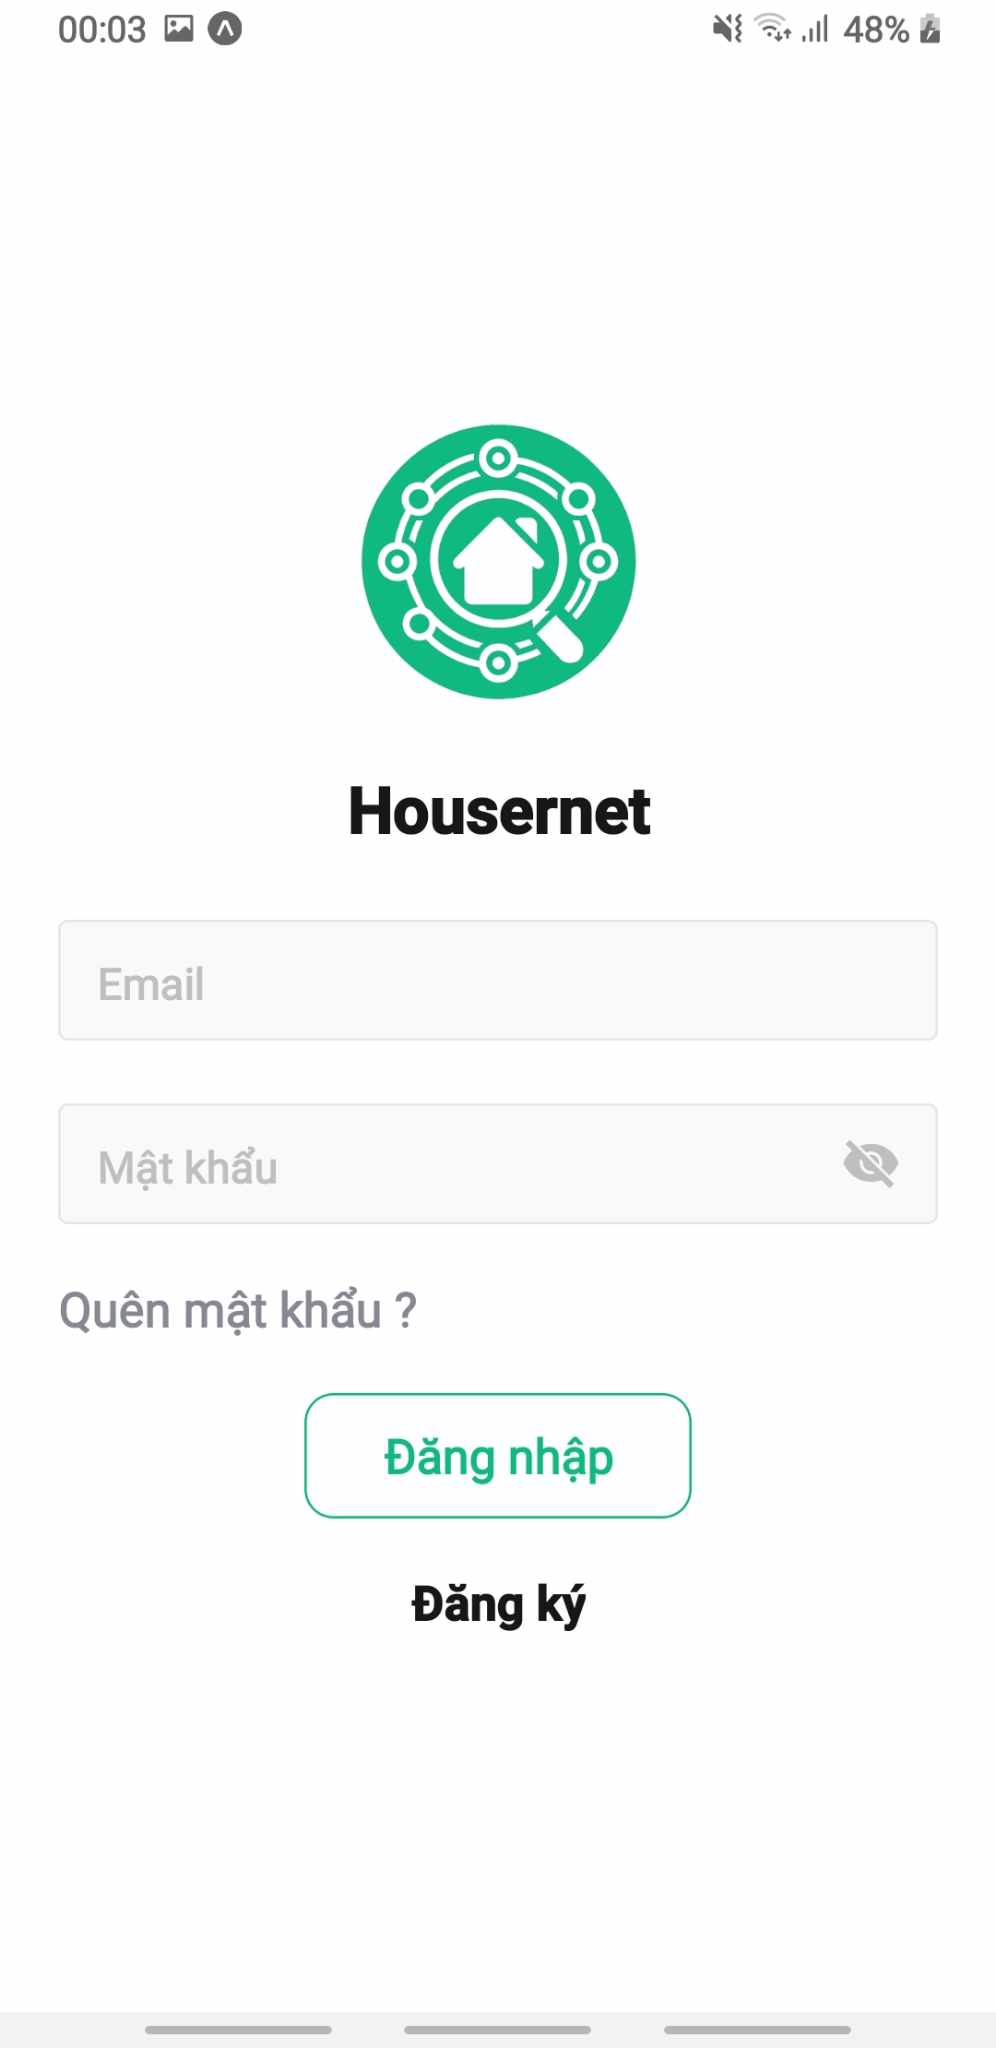
\includegraphics[width=0.5\textwidth]{Images/app_image/app_6.jpg}
    \caption{Đăng nhập}
\end{figure}
Đây là màn hình đầu tiên mà người dùng nhìn thấy khi mở ứng dụng, tại đây yêu cầu người dùng nhập username và password để tiến hành đăng nhập và sử dụng ứng dụng
\subsection{Đăng ký}
\begin{figure}[H]
    \centering
    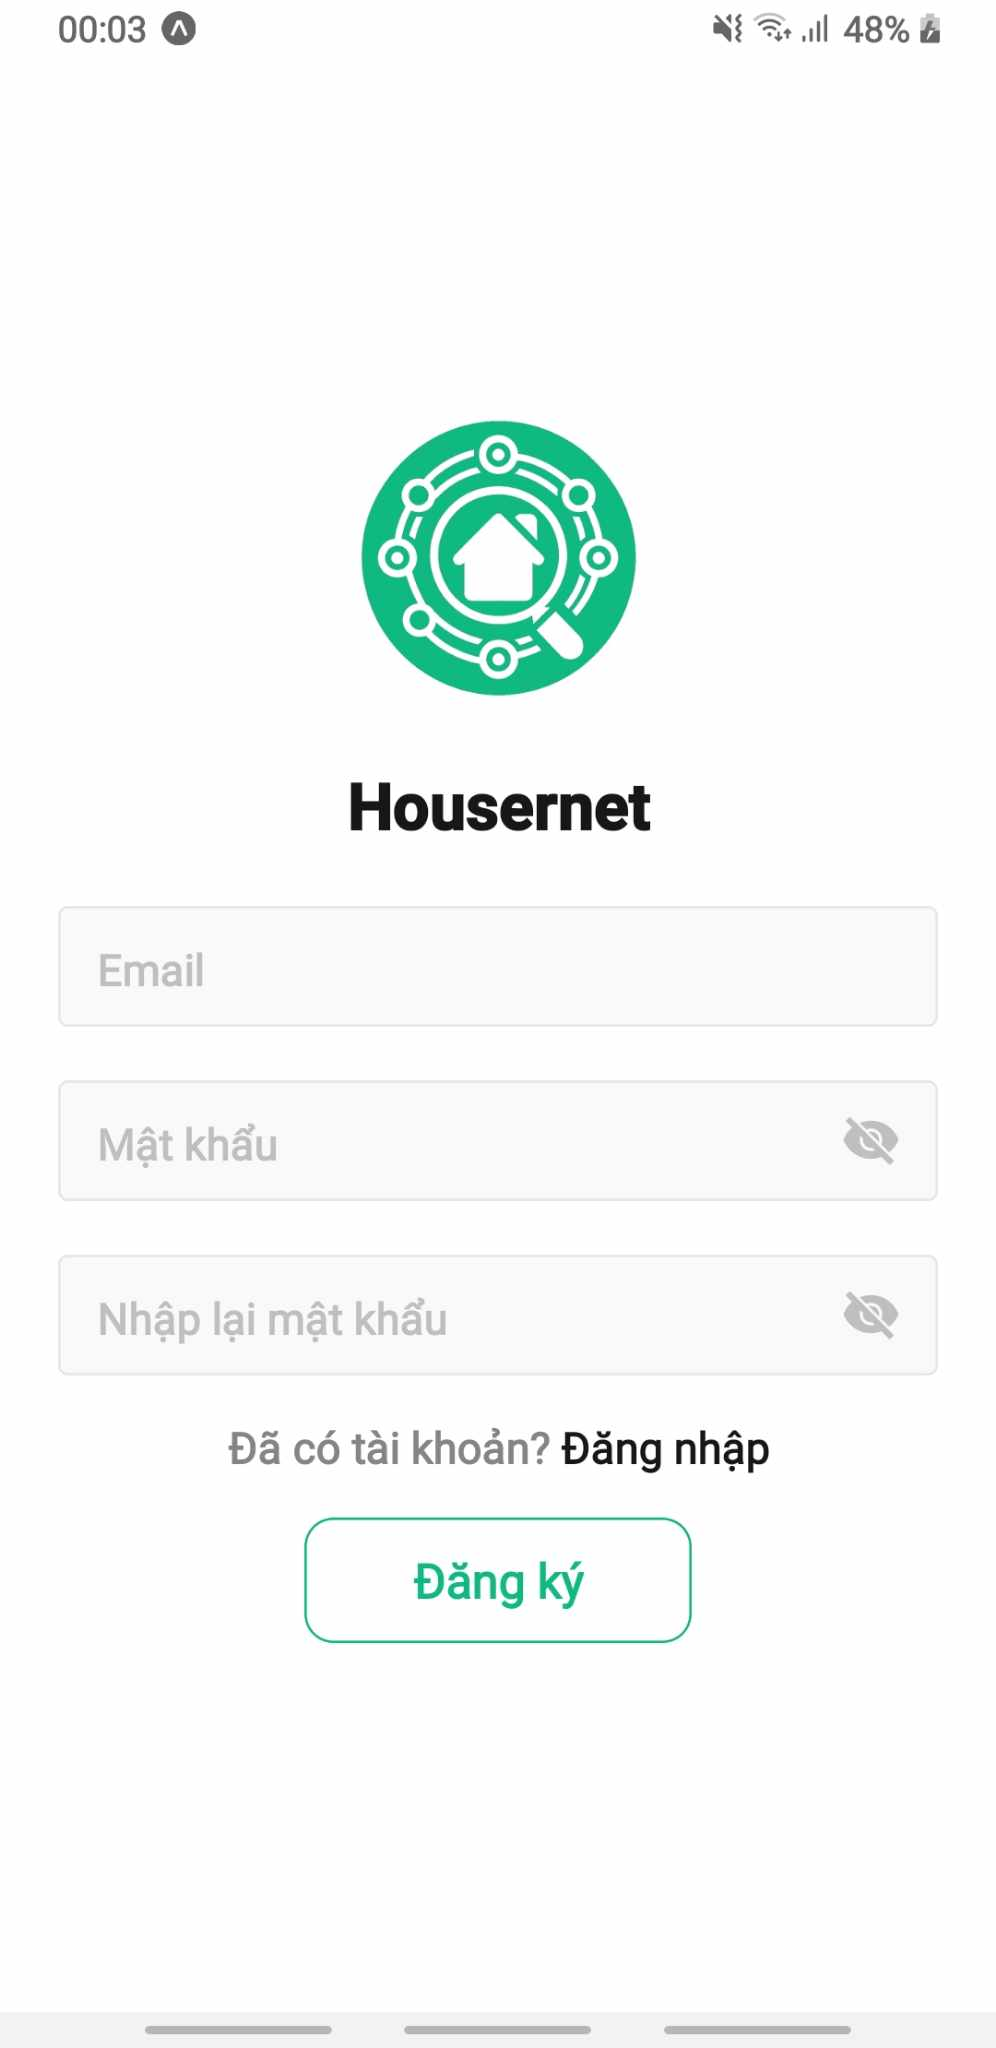
\includegraphics[width=0.5\textwidth]{Images/app_image/app_5.jpg}
    \caption{Đăng ký}
\end{figure}
Màn hình đăng ký được thiết kế để hỗ trợ những người dùng lần đầu tiên dùng app, người dùng tiến hành tạo tài khoản tại đây bằng cách thêm các thông tin về username và password là có thể sử dụng được app, những thông tin khác sẽ có thể bổ sung sau ở profile sau khi đăng nhập thành công
\subsection{Home}
\begin{figure}[H]
    \centering
    \includegraphics[width=0.5\textwidth]{Images/app_image/app_9.jpg}
    \caption{Trang chủ}
\end{figure}
Trang chủ của ứng dụng sẽ gồm các phần như sau :
\begin{itemize}
    \item Thanh search để người dùng có thể nhập câu search tìm nhà theo ý muốn
    \item Nút bộ lọc: để lọc kết quả theo các trường thông tin được cung cấp sẵn trong app
    \item Danh sách nhà trọ được đánh giá cao nhất
    \item Danh sách nhà trọ vừa được cập nhật
\end{itemize}
\subsection{Bộ lọc tìm kiếm}
\begin{figure}[H]
    \centering
    \includegraphics[width=0.5\textwidth]{Images/app_image/app_8.jpg}
    \caption{Bộ lọc tìm kiếm với các trường tìm kiếm theo loại nhà, địa chỉ, giá tiền}
\end{figure}
Bộ lọc tìm kiếm nhà dựa trên các trường thông tin đã được cung cấp trong ứng dụng, chỉ cần chọn rồi chọn filter sẽ ra được danh sách các nhà trùng khớp với thông tin cần filter. Ứng dụng sẽ lọc được các trường thông tin như sau
\begin{itemize}
    \item Địa điểm lọc theo tỉnh thành, quận/huyện và phường xã
    \item Loại nhà mong muốn gồm có : nhà đất, căn hộ, phòng trọ
    \item Các tiện ích như : camera an ninh, tủ lạnh, tv,...
    \item Khung giá tiền của nhà thuê
\end{itemize}
\subsection{Trang tìm kiếm}
\begin{figure}[H]
    \centering
    \includegraphics[width=0.5\textwidth]{Images/app_image/app_7.jpg}
    \caption{Trang tìm kiếm và kết quả trả về}
\end{figure}
Danh sách các nhà tìm được ứng với những từ khóa nhập vào trong thanh search sẽ cho ra, ví dụ ở hình trên khi nhập từ khóa \"Nguyen trai\", danh sách sẽ trả về danh sách các nhà có liên quan đến từ khóa "Nguyen trai" như nằm trên đường nguyễn trãi, hoặc nằm gần nguyễn 
\subsection{Trang chi tiết}
\begin{figure}[H]
    \centering
    \includegraphics[width=0.5\textwidth]{Images/app_image/app_12.jpg}
    \caption{Trang chi tiết của từng nhà trọ}
\end{figure}
Trang chi tiết của từng nhà sẽ có các thông tin như tên, hình ảnh, địa điểm, chủ cho thuê,diện tích, số lượng các phòng, danh sách bình luận,...
\subsection{Bình luận}
\begin{figure}[H]
    \centering
    \includegraphics[width=0.5\textwidth]{Images/app_image/app_11.jpg}
    \caption{Danh sách bình luận trong từng nhà trọ tại trang chi tiết}
\end{figure}
Danh sách các bình luận trong đó mỗi bình luận bao gồm tên người dùng, đánh giá của họ với nhà
\subsection{Trang Profile}
\begin{figure}[H]
    \centering
    \includegraphics[width=0.5\textwidth]{Images/app_image/app_4.jpg}
    \caption{Trang profile thông tin của người dùng}
\end{figure}
\subsection{Danh sách nhà sỡ hữu}\begin{figure}[H]
    \centering
    \includegraphics[width=0.5\textwidth]{Images/app_image/app_3.jpg}
    \caption{Danh sách nhà mà người dùng sở hữu}
\end{figure}
Danh sách các nhà do người dùng đó sở hữu, khi chọn một nhà bất kỳ sẽ hiện lên một tab gồm các chức năng như
\begin{itemize}
    \item Không chọn nhà đó nữa
    \item Xem chi tiết
    \item Chỉnh sửa
    \item Xóa
\end{itemize}
\subsection{Đăng tải nhà mới}
\begin{figure}[H]
    \centering
    \includegraphics[width=0.5\textwidth]{Images/app_image/app_10.jpg}
    \caption{Đăng tải nhà mới}
\end{figure}
Đăng tải nhà mới lên ứng dụng , người dùng sẽ nhập những thông tin mới thêm hình ảnh, chọn loại hình cho thuê, diện tích, số phòng ngủ, vệ sinh và địa điểm
\subsection{Chỉnh sửa nhà trọ}
\begin{figure}[H]
    \centering
    \includegraphics[width=0.5\textwidth]{Images/app_image/app_2.jpg}
    \caption{Chỉnh sửa nhà trong danh sách các nhà trọ}
\end{figure}
Tương tự như đăng nhà mới, cũng có các trường thông tin có sẵn
\subsection{Xóa nhà sỡ hữu}
\begin{figure}[H]
    \centering
    \includegraphics[width=0.5\textwidth]{Images/app_image/app_1.jpg}
    \caption{Xóa nhà trong danh sách nhà trọ}
\end{figure}
Khi chọn nhà cho thuê, ứng dụng sẽ hiển thị lên option để xóa, chọn xóa sẽ hiện lên một thông báo như hình, sau khi chọn xóa, nhà sẽ được xóa khỏi ứng dụng
\newpage


\chapter{TRIỂN KHAI HỆ THỐNG}
\section{TRIỂN KHAI CƠ SỞ DỮ LIỆU}
\subsection{Tổng quan về Aiven - Dịch vụ đám mây cơ sở dữ liệu}
\hspace*{1cm}
Khi triển khai một hệ thống cũng như ứng dụng, bước đầu tiên luôn là triển khai với cơ sở dữ liệu vì cơ sở dữ liệu đóng vai trò then chốt trong việc lưu trữ và quản lý thông tin. Cơ sở dữ liệu là nơi lưu trữ tất cả dữ liệu quan trọng mà ứng dụng cần để hoạt động, bao gồm thông tin người dùng, các giao dịch, và các cấu hình hệ thống. Bằng cách thiết lập cơ sở dữ liệu trước, nhà phát triển đảm bảo rằng mọi thành phần khác của ứng dụng có một nền tảng vững chắc để truy cập và xử lý dữ liệu. Điều này giúp giảm thiểu rủi ro lỗi và tăng cường hiệu suất khi tích hợp các chức năng khác của ứng dụng. Việc triển khai cơ sở dữ liệu từ sớm cũng là bước quan trọng để tất cả mọi người khi phát triển hệ thống sẽ đảm bảo được việc đồng nhất dữ liệu giữa các bên, đảm bảo tính đúng đắn của dữ liệu đối với các tác vụ đọc, thêm, sửa hoặc xóa, giúp cho quá trình phát triển hệ thống trong nhóm được hiệu quả hơn. Ngoài ra, việc triển khai cơ sở dữ liệu sớm còn cho phép kiểm thử và tối ưu hóa các truy vấn dữ liệu, đảm bảo rằng hệ thống hoạt động một cách hiệu quả và mượt mà ngay từ đầu.\\
\hspace*{1cm}
Hiện nay, có rất nhiều dịch vụ đám mây để triển khai cơ sở dữ liệu, bao gồm các dịch vụ miễn phí và có trả phí, nhưng nổi trội hơn hết vẫn là ba dịch vụ đám mây hàng đầu thế giới đó là \textit{Google Cloud}, \textit{Microsoft Azure} và \textit{Amazon Web Services}. Tuy nhiên ba dịch vụ trên đòi hỏi các bước cấu hình phức tạp khi triển khai cơ sở dữ liệu, mặc dù cả ba dịch vụ đều có hỗ trợ triển khai miễn phí tuy nhiên khả năng sử dụng lại khá hạn chế. Cho nên trong phạm vi đề tài này, sau khi đã tìm hiểu qua các dịch vụ triển khai cơ sở dữ liệu, nhóm quyết định sử dụng dịch vụ triển khai do \textit{Aiven} cung cấp. \textit{Aiven} là một nền tảng quản lý cơ sở hạ tầng dữ liệu đám mây toàn diện, cung cấp một loạt các dịch vụ cơ sở dữ liệu và dữ liệu thời gian thực như \textit{PostgreSQL}, \textit{MySQL}, \textit{Cassandra}, \textit{Redis}, \textit{Kafka}, \textit{Elasticsearch}, và nhiều dịch vụ khác. Với \textit{Aiven}, đội ngũ phát triển có thể triển khai, quản lý và mở rộng các dịch vụ dữ liệu một cách dễ dàng và hiệu quả trên các nhà cung cấp đám mây hàng đầu như \textit{AWS}, \textit{Google Cloud}, \textit{Microsoft Azure} và \textit{DigitalOcean} mà không cần lo lắng về việc quản lý cơ sở hạ tầng phức tạp. Các lợi ích chính khi triển khai cơ sở dữ liệu trên \textit{Aiven Cloud} có thể kể đến như:
\begin{itemize}
    \item \textit{Triển khai nhanh chóng:} \textit{Aiven} cho phép người dùng triển khai các dịch vụ dữ liệu chỉ trong vài phút. Điều này giúp tiết kiệm thời gian và tài nguyên, cho phép các đội ngũ phát triển tập trung vào phát triển ứng dụng thay vì phải lo lắng về việc thiết lập và cấu hình cơ sở dữ liệu.
    \item \textit{Quản lý dễ dàng:} Với giao diện người dùng thân thiện và \textit{API} mạnh mẽ, \textit{Aiven} giúp quản lý các dịch vụ dữ liệu trở nên dễ dàng hơn bao giờ hết. Các tính năng như sao lưu tự động, cập nhật phần mềm, và giám sát hiệu suất được tích hợp sẵn, giúp đảm bảo hệ thống luôn hoạt động một cách tối ưu mà không cần sự can thiệp phức tạp từ phía người dùng.
    \item \textit{Khả năng mở rộng linh hoạt:} \textit{Aiven} hỗ trợ mở rộng quy mô dịch vụ dữ liệu một cách linh hoạt. Đội ngũ phát triển có thể dễ dàng điều chỉnh tài nguyên dựa trên nhu cầu thực tế, cho phép mở rộng hoặc thu nhỏ quy mô dịch vụ mà không gây gián đoạn cho hoạt động của hệ thống.
    \item \textit{Hỗ trợ đa dịch vụ đám mây:} \textit{Aiven} cho phép triển khai các dịch vụ trên nhiều nhà cung cấp đám mây khác nhau. Điều này không chỉ tăng tính linh hoạt mà còn giúp cải thiện khả năng phục hồi của hệ thống, đảm bảo rằng dịch vụ luôn sẵn sàng ngay cả khi có sự cố xảy ra ở một nhà cung cấp đám mây nào đó.
    \item \textit{Giảm thiểu sự phức tạp}: \textit{Aiven} loại bỏ nhu cầu phải quản lý cơ sở hạ tầng phức tạp, cho phép các đội ngũ phát triển tập trung vào việc phát triển ứng dụng và dịch vụ. Điều này không chỉ giúp tiết kiệm thời gian mà còn giảm bớt gánh nặng quản lý cho các đội ngũ kỹ thuật.
    \item \textit{Hiệu suất và độ tin cậy:} Với các tính năng như sao lưu tự động, giám sát hiệu suất và cập nhật phần mềm tự động, \textit{Aiven} đảm bảo rằng các dịch vụ dữ liệu luôn hoạt động ở mức hiệu suất cao nhất. Điều này giúp cải thiện độ tin cậy và tính sẵn sàng của hệ thống, đảm bảo rằng hệ thống không bị gián đoạn trong quá trình vận hành.
    \item \textit{Bảo mật dữ liệu:} Các tính năng bảo mật mạnh mẽ của \textit{Aiven} giúp bảo vệ dữ liệu quan trọng của đội ngũ phát triển. Việc tuân thủ các tiêu chuẩn bảo mật nghiêm ngặt và hỗ trợ các công cụ xác thực hiện đại giúp ngăn chặn các cuộc tấn công và rủi ro bảo mật, đảm bảo rằng dữ liệu luôn an toàn.
    \item \textit{Lợi ích chi phí:} Bằng cách cung cấp một nền tảng quản lý dịch vụ dữ liệu toàn diện, Aiven giúp đội ngũ phát triển tối ưu hóa chi phí. Việc không cần đầu tư vào cơ sở hạ tầng phần cứng và giảm bớt yêu cầu về nhân lực kỹ thuật giúp giảm chi phí vận hành tổng thể.
\end{itemize}
\subsection{Thực hiện triển khai cơ sở dữ liệu PostgreSQL}
\hspace*{1cm}
Trong phạm vi đề tài này, nhóm sử dụng gói dùng thử \textit{Aiven Cloud} và được cung cấp số tiền là \$300.0 để sử dụng các dịch vụ. Tận dụng ưu thế này, nhóm đã sử dụng gói \textit{Startup-4} của \textit{Aiven} để triển khai cấu hình hạ tầng cho dịch vụ cơ sở dữ liệu \textit{PostgreSQL}, nhóm triển khai hạ tầng \textit{DigitalOcean} với cấu hình như sau:
\begin{itemize}
    \item \textit{CPU:} 2 \textit{CPU} cho mỗi máy ảo
    \item \textit{RAM:} 4GB \textit{RAM}
    \item \textit{Lưu trữ:} Đối với hệ quản trị cơ sở dữ liệu \textit{PostgreSQL} và \textit{MySQL}, \textit{Aiven} cung cấp dung lượng lưu trữ là 80GB.
    \item \textit{Giám sát:} Giám sát với \textit{metric} và \textit{log}
    \item \textit{Sao lưu dữ liệu:} Hỗ trợ phục hồi tại bất cứ thời điểm nào trong vòng 48 tiếng trở lại.
    \item \textit{Hạ tầng triển khai:} \textit{DigitalOcean} với rất nhiều khu vực phổ biến trên thế giới. Ở đây nhóm chọn triển khai hạ tầng ở \textit{Singapore}.
\end{itemize}
\hspace*{1cm}
Để triển khai cơ sở dữ liệu, ta cần bắt đầu với việc khởi tạo một dự án mới trong \textit{Aiven Cloud}. Mỗi dự án trong \textit{Aiven Cloud} sẽ giúp quản lý các dịch vụ được triển khai bên trong nó, thường là các dịch vụ chung cho một dự án cụ thể.
\begin{figure}[H]
    \centering
    \includegraphics[width=1\textwidth]{Images/Deployment/Database/AivenProject.png}
    \caption{Khởi tạo dự án trong Aiven Cloud}
\end{figure}
\hspace*{1cm}
Bước tiếp theo sau khi khởi tạo dự án đó là cần khởi tạo dịch vụ triển khai cơ sở dữ liệu, ở đây nhóm thực hiện triển khai dịch vụ cơ sở dữ liệu \textit{PostgreSQL}. Ở trong dự án, ta cần chọn \textit{Create service} và thiết lập các cấu hình cần thiết ở các bước tiếp theo.
\begin{figure}[H]
    \centering
    \includegraphics[width=1\textwidth]{Images/Deployment/Database/AivenConfiguration.png}
    \caption{Cấu hình khi triển khai cơ sở dữ liệu với Aiven Cloud}
\end{figure}
\hspace*{1cm}
Sau khi khởi tạo thành công dịch vụ, các bước còn lại là việc \textit{Aiven Cloud} sẽ thực hiện khởi tạo các cấu hình cho dịch vụ triển khai trên hạ tầng mà người dùng đã lựa chọn ở bước cấu hình. Ở bước này, ta cần chờ để hạ tầng thực hiện các bước cần thiết để máy chủ của dịch vụ có thể hoạt động. Sau một thời gian ngắn, dịch vụ cơ sở dữ liệu sẽ sẵn sàng để hoạt động.
\begin{figure}[H]
    \centering
    \includegraphics[width=1\textwidth]{Images/Deployment/Database/AivenRunning.png}
    \caption{Dịch vụ cơ sở dữ liệu Aiven Cloud trong trạng thái sẵn sàng kết nối}
\end{figure}
\hspace*{1cm}
Sau khi đã dịch vụ đã sẵn sàng, ta có thể kiểm tra trạng thái hoạt động của dịch vụ thông qua việc thiết lập kết nối. Ở đây ta sử dụng công cụ \textit{DataGrip}, như đã đề cập ở phía trên thì công cụ này giúp nhà phát triển có thể dễ dàng làm việc trên các cơ sở dữ liệu khác nhau. Để thiết lập kết nối với dịch vụ cơ sở dữ liệu, ở giao diện của \textit{DataGrip}, ta sẽ chọn nút dấu cộng \textit{+} ở góc bên trái phía trên và chọn \textit{Data Source}, lúc này giao diện sẽ hiển thị các loại cơ sở dữ liệu khác nhau mà \textit{DataGrip} có hỗ trợ, đến đây ta sẽ chọn \textit{PostgreSQL}. Một bảng \textit{pop-up} sẽ hiện ra và ở đây ta sẽ cần cung cấp các thông tin liên quan đến dịch vụ cơ sở dữ liệu bao gồm \textit{hostname}, \textit{port}, \textit{username}, \textit{password} và \textit{database}, sau đó ta sẽ nhấn vào \textit{Test Connection} để kiểm tra trạng thái kết nối.
\begin{figure}[H]
    \centering
    \includegraphics[width=0.8\textwidth]{Images/Deployment/Database/SuccessfulConnection.png}
    \caption{Bảng thông báo cho thấy kết nối từ DataGrip và dịch vụ Aiven Cloud đã được thiết lập thành công}
\end{figure}

\section{TRIỂN KHAI BACK-END}
\subsection{Tổng quan về Vercel - Dịch vụ điện toán phi máy chủ}
\hspace*{1cm}
Sau khi đã triển khai thành công dịch vụ cơ sở dữ liệu trên \textit{Aiven Cloud}. Bước tiếp theo trong quá trình triển khai hệ thống đó là ta cần triển khai ở phía \textit{back-end}. Việc triển khai \textit{back-end} được thực hiện song song với quá trình phát triển mã nguồn, được gọi là quá trình triển khai liên tục \textit{(Continuous Deployment - CD)}. Việc thực hiện triển khai liên tục là điều cần thiết trong hầu hết các dự án phần mềm. Trước hết việc triển khai liên tục cho phép đội ngũ phát triển ở phía \textit{front-end} có thể dễ dàng tích hợp \textit{API} vào trong ứng dụng \textit{front-end} mà không cần phải chạy ứng dụng \textit{back-end} ở phía \textit{local}. Việc tích hợp liên tục cho phép nhà phát triển \textit{back-end} nhanh chóng cung cấp \textit{API} cho các chức năng bên phía \textit{front-end}. Ngoài ra triển khai liên tục cũng cải thiện chất lượng phần mềm thông qua việc áp dụng các quy trình kiểm tra tự động liên tục. Bằng cách phát hiện sớm các lỗi trong quá trình phát triển, các lỗi này có thể được khắc phục ngay lập tức, giảm thiểu rủi ro và chi phí liên quan đến việc sửa lỗi trong giai đoạn sau của vòng đời phần mềm. Hơn nữa, việc triển khai liên tục giúp các nhóm phát triển phản ứng linh hoạt hơn với phản hồi của các bên liên quan bao gồm phía đội ngũ \textit{front-end} cũng như phía người dùng, để từ đó đội ngũ \textit{back-end} có thể nhanh chóng cập nhật các thay đổi và đưa các thay đổi đó lên ứng dụng một cách trơn tru nhất.\\
\hspace*{1cm}
Hiện nay, có rất nhiều đơn vị cung cấp dịch vụ đám mây để triển khai \textit{Web API}, bao gồm các dịch vụ miễn phí cũng như trả phí. Trong đó có các nền tảng dịch vụ đám mây quen thuộc được sử dụng phổ biến nhất là \textit{Google Cloud}, \textit{Microsoft Azure} và \textit{Amazon Web Services}. Các dịch vụ triển khai thường theo hai dạng chính đó là \textit{serverful} và \textit{serverless}. Serverful là một dạng triển khai đám mây trong đó nhà phát triển và tổ chức phải quản lý cơ sở hạ tầng máy chủ, điều này bao gồm thiết lập, cấu hình, và bảo trì máy chủ vật lý hoặc ảo. Trong khi đó ở hướng ngược lại, serverless là một cách triển khai trong đó nhà cung cấp dịch vụ đám mây tự động quản lý cơ sở hạ tầng máy chủ. Các nhà phát triển viết mã ứng dụng và triển khai nó mà không cần quan tâm đến việc thiết lập, quản lý hoặc bảo trì các máy chủ. Trong phạm vi dự án này, nhóm sẽ thực hiện triển khai \textit{back-end} theo hướng serverless. Điều này sẽ đem lại những lợi ích nhất định có thể kể đến là:
\begin{itemize}
    \item \textit{Không cần quản lý server:} Nhà cung cấp dịch vụ đám mây chịu trách nhiệm về cơ sở hạ tầng. Nhà phát triển chỉ cần tập trung vào viết mã.
    \item \textit{Có thể tự động mở rộng:} Ứng dụng có thể tự động mở rộng để đáp ứng nhu cầu tải, mà không cần cấu hình thêm máy chủ thủ công.
    \item \textit{Chi phí thanh toán dựa trên mức độ sử dụng}: Bạn chỉ phải trả tiền cho thời gian thực thi mã của mình, không phải cho thời gian mà máy chủ nhàn rỗi.
    \item \textit{Thời gian khởi động nhanh:} Vì cơ sở hạ tầng được quản lý động, thời gian khởi động ứng dụng thường rất nhanh.
\end{itemize}
\hspace*{1cm}
Ở đây nhóm sẽ sử dụng dịch vụ \textit{Vercel}, Vercel là một nền tảng đám mây được thiết kế để triển khai và lưu trữ các ứng dụng web và front-end một cách nhanh chóng và dễ dàng. Nó cung cấp dịch vụ triển khai liên tục tự động, cho phép nhà phát triển đẩy mã mới lên kho lưu trữ và \textit{Vercel} sẽ tự động triển khai nó lên môi trường sản phẩm. \textit{Vercel} được xây dựng dựa trên mạng lưới toàn cầu của \textit{Edge servers}, giúp mang lại hiệu suất cao và độ trễ thấp cho người dùng toàn cầu, các lợi ích mà \textit{vercel} đem lại có thể kể đến như:
\begin{itemize}
    \item \textit{Triển khai ứng dụng web:} \textit{Vercel} có thể triển khai các ứng dụng \textit{web} tĩnh, ứng dụng \textit{React}, ứng dụng \textit{Vue.js}, \textit{Svelte} và các ứng dụng \textit{Node.js}.
    \item \textit{Lưu trữ tệp tĩnh:} \textit{Vercel} có thể lưu trữ và phân phối các tệp tĩnh như hình ảnh, \textit{CSS} và \textit{JavaScript}.
    \item \textit{Mạng CDN toàn cầu:} \textit{Vercel} sử dụng mạng \textit{CDN} toàn cầu để phân phối nội dung ứng dụng của nhà phát triển đến người dùng trên toàn thế giới một cách nhanh chóng và hiệu quả.
    \item \textit{Tên miền tùy chỉnh:} Nhà phát triển có thể sử dụng tên miền tùy chỉnh cho ứng dụng \textit{Vercel} của mình.
    \item \textit{HTTPS:} \textit{Vercel} hỗ trợ \textit{HTTPS} cho tất cả các ứng dụng.
    \item \textit{Analytics:} \textit{Vercel} cung cấp \textit{analytics} tích hợp để theo dõi lưu lượng truy cập và hiệu suất ứng dụng.
\end{itemize}
\subsection{Thực hiện triển khai back-end trên Vercel}
\hspace*{1cm}
Bước đầu tiên, ta cần có tài khoản \textit{Vercel} và thực hiện liên kết tài khoản tới trình quản lý \textit{Git}, có thể là \textit{GitHub}, \textit{GitLab} hoặc \textit{BitBucket}, ngoài ra cũng có thể thực hiện liên kết với trình quản lý \textit{Git} của bên thứ ba. Sau đó ở thư mục chứa mã nguồn \textit{back-end}, ta cần tạo một file đặt tên là \textit{vercel.json} để thiết lập cấu hình trước khi triển khai trên \textit{Vercel}. Dưới đây là đoạn mã cấu hình trong dự án \textit{back-end} của nhóm:
\begin{lstlisting}[language=json,firstnumber=1]
{
    "version": 2,
    "builds": [
        {
            "src": "src/main.ts",
            "use": "@vercel/node"
        }
    ],
    "routes": [
        {
            "src": "/(.*)",
            "dest": "src/main.ts",
            "methods": ["GET", "POST", "PUT", "PATCH", "DELETE", "OPTIONS"],
            "headers": {
                "Access-Control-Allow-Origin": "*"
            }
        }
    ]
}
\end{lstlisting}
\hspace*{1cm}
Bước tiếp theo, vì ta sử dụng \textit{Prisma ORM} để làm việc với cơ sở dữ liệu, nên sẽ cần thiết lập câu lệnh sẽ được chạy khi \textit{Vercel} thực hiện \textit{build} dự án để sinh ra được \textit{prisma client} trên \textit{Vercel}. Ở đây ta cần đề cập đến cơ chế hoạt động của \textit{Prisma ORM}, sau khi đặc tả các bảng và quan hệ trong \textit{file schema.prisma}, ta cần chạy câu lệnh \textit{prisma push} để đồng bộ với cơ sở dữ liệu ở trên \textit{server}. Khi thực hiện câu lệnh \textit{prisma push}, \textit{Prisma} cũng đồng thời thực thi câu lệnh \textit{prisma generate} để sinh ra \textit{prisma client} nằm ở trong thư mục của dự án. \textit{Prisma client} có thể được hiểu là \textit{API} trung gian mà \textit{Prisma} cung cấp để phía \textit{back-end} có thể giao tiếp được với cơ sở dữ liệu. Do vậy khi triển khai dự án trên \textit{Vercel}, ta cũng cần phải thiết lập để câu lệnh \textit{prisma generate} có thể thực thi đồng thời với quá trình \textit{build} dự án. Để làm được điều này ta cần chỉnh sửa ở \textit{file package.json} trong mã nguồn như sau:
\begin{lstlisting}[language=json,firstnumber=1]
{
    //...
    "scripts": {
        "build": "npm run generate-prisma-client-on-build && nest build",
        //...
        "generate-prisma-client-on-build": "prisma generate --schema prisma/schema.prisma",
        "vercel-build": "npm run build"
    }
    //...
}
\end{lstlisting}
\hspace*{1cm}
Đến đây ta đã thực hiện chỉnh sửa xong mã nguồn để sẵn sàng triển khai trên \textit{Vercel}, bước tiếp theo khá quen thuộc đó là ta cần \textit{commit} và \textit{push} những thay đổi mà ta đã thực hiện ở phía trên lên trên \textit{GitHub}. Sau khi đã thực hiện xong, ta sẽ truy cập vào trang chủ của \textit{Vercel} và khởi tạo một dự án triển khai mới. Trước tiên ta cần chọn tên của \textit{GitHub repository} tương ứng với dự án cần triển khai, sau đó nhấn vào \textit{Import}, lúc này \textit{Vercel} sẽ hiển thị giao diện để thực hiện các cấu hình cần thiết trước khi triển khai dự án. Tại bước thiết lập này, ta sẽ cần đặt tên cho dự án triển khai ở mục \textit{Project Name}, chọn \textit{framework} ứng với dự án, vì ở đây ta triển khai dự án \textit{NestJS} nên không có tùy chọn tương ứng, do đó ở mục \textit{Framework Preset} ta sẽ chọn \textit{Other}. Tiếp theo ở mục \textit{Root Directory}, ta cần trỏ tới thư mục chứa toàn bộ mã nguồn của dự án, mặc định ta không cần thay đổi ở mục này, tuy nhiên với \textit{Git repository} mà có chứa nhiều dự án khác thì ta cần thiết lập cho chính xác. Tiếp theo cần thiết lập ở mục \textit{Build and Output Settings}, vì đây là dự án \textit{NestJS} nên ở mục này ta không cần tùy chỉnh, tuy nhiên cần lưu ý với các dự án khác nhau. Cuối cùng ta cần thêm các biến môi trường của dự án ở mục \textit{Environment Variables}, chúng ta có thể thêm một cách tiện lợi đó là \textit{copy} toàn bộ \textit{file .env} trong dự án và \textit{paste} vào ô đầu tiên của mục này, tất cả các biến môi trường sẽ tự động được \textit{import}.
\begin{figure}[H]
    \centering
    \includegraphics[width=1\textwidth]{Images/Deployment/Backend/VercelConfig.png}
    \caption{Thiết lập cấu hình trước khi triển khai dự án trên Vercel}
\end{figure}
\hspace*{1cm}
Sau khi đã hoàn tất các bước ở trên, ta sẽ nhấn vào \textit{Deploy} để \textit{Vercel} tiến hành triển khai ứng dụng, để theo dõi quá trình \textit{build}, ta có thể quan sát ở mục \textit{Deployment Details}, tại mục này sẽ hiển thị các tiến trình \textit{Vercel} thực hiện \textit{build} và triển khai ứng dụng, ta có thể nhấn vào chi tiết để xem các câu lệnh được chạy trong quá trình \textit{build}, nhờ đó ta có thể theo dõi quá trình \textit{build} có thành công hay không, hoặc nếu xảy ra lỗi, ta có thể xem \textit{build log} để tìm ra nguyên nhân gây ra lỗi khi \textit{build} ứng dụng.
\begin{figure}[H]
    \centering
    \includegraphics[width=1\textwidth]{Images/Deployment/Backend/DeploymentDetail.png}
    \caption{Các bước build ứng dụng trên Vercel}
\end{figure}
\begin{figure}[H]
    \centering
    \includegraphics[width=1\textwidth]{Images/Deployment/Backend/BuildLog.png}
    \caption{Build log hiển thị các câu lệnh được thực thi khi Vercel build ứng dụng}
\end{figure}
\hspace*{1cm}
Khi khởi tạo dự án triển khai trên \textit{Vercel}, ở lần \textit{build} đầu tiên, \textit{Vercel} sẽ cung cấp một tên miền với cấu trúc là \url{[project-name].vercel.app}. Sau khi quá trình \textit{build} thành công và không gặp bất cứ lỗi nào, kết quả thành công sẽ được hiển thị trên giao diện chính của dự án, và ta có thể sử dụng tên miền mà \textit{Vercel} cung cấp để tích hợp ở phía \textit{front-end}. Ngoài ra ta cũng có thể truy cập vào \textit{tab Log} để theo dõi ứng dụng hoạt động.
\begin{figure}[H]
    \centering
    \includegraphics[width=1\textwidth]{Images/Deployment/Backend/SuccessfullyBuilt.png}
    \caption{Kết quả sau khi build ứng dụng thành công trên Vercel}
\end{figure}
\section{TRIỂN KHAI MÔ HÌNH HYBRID SEARCH}
\subsection{Tổng quan về Azure VM - Nền tảng máy ảo triển khai ứng dụng}
\hspace*{1cm}
Bước tiếp theo trong quá trình triển khai, ta cần thực hiện việc triển khai mô hình hybrid search. Do đây là mô hình khá nặng về dung lượng cũng như cần tài nguyên tính toán cao nên cần được triển khai trên một nền tảng độc lập tách biệt với nền tảng \textit{back-end}. Cách tiếp cận của nhóm khi triển khai mô hình này đó là thực hiện triển khai trên một máy ảo từ xa. Hiện nay, cả ba dịch vụ điện toán đám mây hàng đầu là \textit{Google Cloud}, \textit{Microsoft Azure} và \textit{Amazon Web Services} đều cung cấp dịch vụ cho thuê máy ảo, hỗ trợ tốt các hệ điều hành phổ biến hiện nay như \textit{Windows} hay \textit{Linux}. Sau khi đã xem xét và tìm hiểu, nhóm quyết định chọn triển khai với máy ảo với dịch vụ của \textit{Microsoft Azure}. Các lợi ích có thể kể đến mà máy ảo do \textit{Microsoft Azure} cung cấp đó là:
\begin{itemize}
    \item \textit{Tính linh hoạt và mở rộng:} \textit{Azure} cung cấp khả năng mở rộng linh hoạt, cho phép người sử dụng dễ dàng tăng hoặc giảm tài nguyên máy ảo theo nhu cầu kinh doanh. người sử dụng có thể thay đổi cấu hình máy ảo như \textit{CPU}, \textit{RAM}, và dung lượng lưu trữ một cách nhanh chóng.
    \item \textit{Chi phí hiệu quả:} \textit{Azure} cung cấp nhiều tùy chọn giá cả, bao gồm mô hình thanh toán theo mức sử dụng \textit{(pay-as-you-go)}, giúp người sử dụng chỉ phải trả tiền cho những gì người sử dụng sử dụng. Điều này giúp tiết kiệm chi phí và tránh lãng phí tài nguyên.
    \item \textit{Độ tin cậy và hiệu suất cao:} \textit{Azure} đảm bảo mức độ khả dụng cao với các cam kết \textit{SLA (Service Level Agreement)} lên đến 99.95\% cho các máy ảo, đảm bảo rằng ứng dụng và dịch vụ của người sử dụng luôn hoạt động ổn định và hiệu quả.
    \item \textit{Bảo mật mạnh mẽ:} \textit{Azure} tích hợp nhiều tính năng bảo mật như mã hóa dữ liệu, quản lý danh tính và truy cập \textit{(IAM)}, và các công cụ bảo vệ trước các mối đe dọa mạng. \textit{Azure Security Center} giúp người sử dụng theo dõi và quản lý bảo mật toàn diện.
\end{itemize}
\subsection{Thực hiện triển khai mô hình hybrid search trên máy ảo Azure VM}
\hspace*{1cm}
Để bắt đầu việc thực hiện triển khai mô hình trên nền tảng máy ảo \textit{Azure VM}, bước đầu tiên ta cần có tài khoản \textit{Microsoft}, để hưởng chính sách ưu đãi dành cho học sinh, sinh viên, ta có thể sử dụng địa chỉ \textit{email} do trường cung cấp để đăng ký. Ưu đãi đó bao gồm việc sử dụng đa dạng các dịch vụ miễn phí trong vòng một năm, ngoái ra tài khoản cũng sẽ được cung cấp sẵn \$100.0 để mua thêm các dịch vụ nâng cao để sử dụng. Sau khi đã có tài khoản \textit{Microsoft}, ta sẽ cần truy cập vào trang chủ của \textit{Microsoft Azure} và thực hiện bước đầu tiên là tạo ra một \textit{Resource Group}, đây được hiểu là một môi trưởng tài nguyên được triển khai một cách độc lập bao gồm các dịch vụ hoạt động bên trong môi trường này, và được triển khai ở một vùng nhất định trên thế giới, nơi có đặt trung tâm dữ liệu của \textit{Microsft}. Ở đây nhóm thực hiện tạo một \textit{Resource Group} với tên là \textit{ResourceGroup-Primary}, được triển khai ở máy chủ đặt tại \textit{Singapore}.
\begin{figure}[H]
    \centering
    \includegraphics[width=1\textwidth]{Images/Deployment/HybridSearch/ResrouceGroup.png}
    \caption{Resource Group với tên là Resource Group được khởi tạo thành công}
\end{figure}
\hspace*{1cm}
Sau khi đã khởi tạo thành công \textit{Resource Group}, ta đã có thể tiến hành việc tạo ra một máy ảo để bắt đầu quá trình triển khai. Trước tiên ta trở vê trang chính của \textit{Microsoft Azure Portal} và chọn \textit{Virtual Machine}. Sau đó, trang chủ sẽ hiển thị giao diện để người dùng thực hiện các bước cấu hình cần thiết trước khi chạy máy ảo.
\begin{figure}[H]
    \centering
    \includegraphics[width=1\textwidth]{Images/Deployment/HybridSearch/Config1.png}
    \caption{Thiết lập cấu hình cho máy ảo Azure VM}
\end{figure}
\begin{figure}[H]
    \centering
    \includegraphics[width=1\textwidth]{Images/Deployment/HybridSearch/Config2.png}
    \caption{Thiết lập cấu hình cho máy ảo Azure VM}
\end{figure}
\begin{figure}[H]
    \centering
    \includegraphics[width=1\textwidth]{Images/Deployment/HybridSearch/Config3.png}
    \caption{Thiết lập cấu hình cho máy ảo Azure VM}
\end{figure}
\hspace*{1cm}
Các bước thiết lập cấu hình máy ảo \textit{Azure VM} có phần hơi phức tạp, cụ thể các bước cấu hình như sau:
\begin{itemize}
    \item \textit{Subscription:} Ở mục này, ta cần chọn gói thuê bao để \textit{Azure} sẽ thực hiện tính phí cho dịch vụ máy ảo. Ở đây, do nhóm đã đăng ký tài khoản học sinh, sinh viên nên sẽ chọn \textit{Azure for Students}.
    \item \textit{Resource Group:} Ở mục này, ta cần chọn nhóm tài nguyên mà ta đã tạo sẵn ở bước trên, trong mục này, nhóm sẽ chọn \textit{ResourceGroup-Primary}.
    \item \textit{Virtual machine name}: Ở mục này, ta cần đặt tên cho máy ảo.
    \item \textit{Region:} Ở mục này, ta cần lựa chọn vị trí máy chủ nơi mà dịch vụ máy ảo sẽ được triển khai, trong mục này nhóm sẽ chọn \textit{(Asia Pacific) Southeast Asia}, vì vị trí này gần với Việt Nam nhất.
    \item \textit{Availability options:} Ở mục này, ta có thể để giữ nguyên lựa chọn mặc định là \textit{Avaiability zone}
    \item \textit{Availability zone:} Ở mục này, ta cần chọn các \textit{zone} để triển khai máy ảo, mặc định sẽ chọn triển khai ở \textit{Zone 1}, ta có thể giữ nguyên mục này.
    \item \textit{Security type:} Ở mục này, mặc định sẽ là \textit{Trusted launch virtual machines}. Các lựa chọn khác nhau ở mục này sẽ xác định mức độ bảo vệ cho máy ảo.
    \item \textit{Image:} Ở mục này, ta cần chọn hệ điều hành cho máy ảo, ở đây nhóm sẽ chọn hệ điều hành \textit{Ubuntu Server 22.04 LTS - x64 Gen2} để triển khai máy ảo.
    \item \textit{VM architecture:} Ở mục này, ta sẽ chọn kiến trúc vi xử lý của máy ảo, mặc định lựa chọn ở mục này sẽ là kiến trúc \textit{x64}.
    \item \textit{Size:} Đây là mục quan trọng, ta cần chọn kích thước cho phần cứng của máy ảo, phần này sẽ quyết định đến giá tiền sử dụng dịch vụ, để đảm bảo khả năng vận hành của mô hình \textit{hybrid search}, cũng như để tiết kiệm chi phí một cách tối ưu, nhóm đã chọn kích thước \textit{Standard\_B2s - 2 vcpus, 4GiB memory}, với giá mà \textit{Azure} ước tính sẽ rơi vào khoảng \$38.54 cho một tháng.
    \item \textit{Authentication type:} Ở mục này, ta cần chọn phương thức xác thực để kết nối đến máy ảo, ở đây nhóm chọn xác thực bằng \textit{SSH}.
    \item \textit{Username:} Ở đây ta cần đặt một tên tài khoản cho bước xác thực khi đến nối đến máy ảo \textit{Azure}.
    \item \textit{SSH pblic key source:} Để thuận tiện hơn, ở mục này ta chọn \textit{Generate new key pair} và đặt tên cho \textit{public key}.
    \item \textit{Public inbound ports:} Ở đây để có thể kết nối đến máy ảo từ \textit{internet}, ta có thể chọn \textit{Allow selected ports} và tương ứng với mục phía dưới \textit{Select inbound ports}, ta có thể để mặc định là \textit{SSH(22)}. Như vậy, máy ảo sẽ có thể được kết nối từ bất kì đâu và sẽ chấp nhận kết nối bằng giao thức \textit{SSH} ở cổng \textit{22}.
\end{itemize}
\hspace*{1cm}
Đến đây, ta có thể chọn \textit{Review + create} để kiểm tra lại một lần nữa tất cả các cài đặt và cấu hình cho máy ảo, sau khi đã hoàn tất. Ta có thể nhấn vào \textit{Create}, và lúc này vì đã chọn ở bước phía trên là \textit{Generate new key pair}, nên trang chủ sẽ hiện một \textit{pop-up} để đề nghị tải xuống \textit{private key} cho bước xác thực \textit{SSH}. Ở bước này, ta cần tải về và lưu trữ \textit{private key} ở một nơi an toàn trên máy tính. Sau khi đã tải về, ta cần cấp quyền \textit{Full control} cho người dùng của hệ điều hành để tránh bị báo lỗi khi thực hiện kết nối với máy ảo.
\begin{figure}[H]
    \centering
    \includegraphics[width=1\textwidth]{Images/Deployment/HybridSearch/ReviewCreate.png}
    \caption{Kiểm tra lại các cài đặt trước khi tạo máy ảo Azure VM}
\end{figure}
\begin{figure}[H]
    \centering
    \includegraphics[width=0.5\textwidth]{Images/Deployment/HybridSearch/FullControl.png}
    \caption{Cấp quyền full control cho SSH private key}
\end{figure}
\hspace*{1cm}
Đến đây ta có thể kết nối đến máy ảo bằng \textit{command line}, ta có thể sử dụng \textit{Windows Powershell} để kết nối đến địa chỉ \textit{IP} của máy ảo với tên đăng nhập và \textit{SSH private key} mà ta đã khởi tạo ở bước trên.
\begin{figure}[H]
    \centering
    \includegraphics[width=1\textwidth]{Images/Deployment/HybridSearch/VM-Connection.png}
    \caption{Khởi tạo kết nối đến máy ảo Azure VM}
\end{figure}
\hspace*{1cm}
Tiếp theo, ta cần phải chạy được ứng dụng trên máy ảo \textit{Azure VM} tương tự như cách ta chạy ở \textit{localhost}. Tuy nhiên, vì ta cần cho phép các kết nối công khai đến ứng dụng \textit{Flask} đang triển khai ở máy ảo này. Có nhiều phương pháp để thực hiện mục tiêu trên, tuy nhiên để cho đơn giản và nhanh chóng, nhóm sử dụng công cụ \textit{ngrok}, \textit{ngrok} là một công cụ phần mềm cho phép người dùng tạo các đường hầm bảo mật từ một mạng công cộng đến một máy tính hoặc thiết bị cụ thể trong mạng cục bộ của người dùng. Công cụ này thường được sử dụng để:
\begin{itemize}
    \item Triển khai và thử nghiệm ứng dụng \textit{web} cục bộ: Ngrok tạo ra một \textit{URL} công cộng (dạng \url{https://<subdomain>.ngrok.io}) cho phép người dùng truy cập trực tiếp vào ứng dụng web chạy trên máy tính cá nhân của người dùng từ bất kỳ đâu trên \textit{internet}.
    \item Phát triển \textit{webhook}: Khi phát triển các dịch vụ \textit{webhook}, như nhận thông báo từ \textit{Stripe}, \textit{GitHub}, hoặc \textit{Slack}, người dùng có thể sử dụng \textit{ngrok} để nhanh chóng nhận và thử nghiệm các yêu cầu \textit{HTTP} từ các dịch vụ này đến máy chủ cục bộ của người dùng.
    \item Chia sẻ dự án nhanh chóng: Người dùng có thể chia sẻ phiên bản đang phát triển của một trang \textit{web} hoặc ứng dụng với đồng nghiệp hoặc khách hàng mà không cần phải triển khai lên một máy chủ công cộng.
\end{itemize}
\hspace*{1cm}
\textit{Ngrok} hoạt động bằng cách chạy một ứng dụng máy khách trên máy tính của người dùng. Ứng dụng này kết nối với các máy chủ của \textit{ngrok} thông qua một kết nối bảo mật. Khi người dùng khởi chạy \textit{ngrok}, nó sẽ tạo ra một \textit{URL} công cộng và chuyển tiếp tất cả các yêu cầu tới \textit{URL} đó đến máy tính cục bộ của người dùng thông qua kết nối bảo mật.\\
\hspace*{1cm}
Để thiết lập \textit{ngrok} trên máy ảo \textit{Azure VM}, ta cần phải có tài khoản \textit{ngrok}, sau đó truy cập vào trang \textit{web} của \textit{ngrok} để lấy mã \textit{token} ứng với tài khoản đang sử dụng. Và sau đó, ở giao diện \textit{command line} của máy ảo \textit{Azure VM}, ta cần chạy câu lệnh:
\begin{lstlisting}
ngrok config add-authtoken <token>
\end{lstlisting}
\hspace*{1cm}
Bước tiếp theo, ta cần thiết lập \textit{ngrok} ở trong mã nguồn của mô hình tìm kiếm \textit{hybrid}, ở bước này, ta cần thêm các dòng sau trong \textit{file app.py}, để mỗi khi ứng dụng \textit{Flask} khởi chạy, ứng dụng sẽ tạo ra một \textit{URL} công khai để bất kì thiết bị nào cũng có thể kết nối đến ứng dụng:
\begin{python}
from pyngrok import ngrok

# Open a ngrok tunnel to the HTTP server
public_url = ngrok.connect(5000).public_url
print(' * ngrok tunnel "{}" -> "http://127.0.0.1:{}/"'.format(public_url, 5000))

# Update any base URLs to use the public ngrok URL
app.config["BASE_URL"] = public_url
\end{python}
\hspace*{1cm}
Cuối cùng, ta cần \textit{commit} và \textit{push} mã nguồn lên \textit{GitHub}, sau đó ta chuyển qua giao diện \textit{command line} của máy ảo \textit{Azure VM} để \textit{clone} mã nguồn về, ở bước này ta cần phải có \textit{Personal access token} của \textit{GitHub}, để lấy được \textit{access token} này, ta cần vào bên trong cài đặt tài khoản cá nhân của \textit{GitHub} để sử dụng. Sau khi ta đã \textit{clone} được mã nguồn thành công, bước tiếp theo ta cần cài đặt các \textit{package} kèm theo của ứng dụng. Sau đó ta cần sử dụng lệnh \textit{tmux} để tạo ra một \textit{command line session} riêng trên máy ảo, ta cần phải làm như vậy để khi ngắt kết nối khỏi máy ảo thì \textit{command line} vẫn tiếp tục chạy như bình thường, và do đó sẽ giúp cho ứng dụng không bị ngưng khi ta thoát khỏi máy ảo. Và cuối cùng, ta chỉ cần chạy câu lệnh \textit{flask run} để khởi động ứng dụng mô hình tìm kiếm \textit{hybrid}. Khi ứng dụng được khởi chạy, giao diện \textit{command line} hiển thị địa chỉ \textit{URL} để truy cập đến ứng dụng, ta cần lưu giữ địa chỉ \textit{URL} này để kết nối về sau. Để thoát ra khỏi \textit{command line} đang chạy ứng dụng, ta cần nhấn tổ hợp phím \textit{Ctrl + B}, sau đó nhấn phím \textit{D}. Như vậy, ta có thể tạm thời ngắt kết nối đến \textit{command line} mà vẫn giữ cho ứng dụng tiếp tục được hoạt động mà không bị dừng. Đến đây, ta đã hoàn thành việc triển khai ứng dụng mô hình tìm kiếm \textit{hybrid} trên máy ảo \textit{Azure VM}
\section{PHÁT HÀNH ỨNG DỤNG}
Đầu tiên để phát hành ứng dụng, cần phải tải thư viện eas-cli để có thể phát hành ứng dụng 
\begin{figure}[H]
    \centering
    \includegraphics[width=1\textwidth]{Images/Build_app/eas_install.png}
    \caption{Tải thư viện eas-cli}
\end{figure}
Ở dự án này sử dụng expo go để phát triển do đó cần phải đăng nhập vào tài khoản để kích hoạt
\begin{figure}[H]
    \centering
    \includegraphics[width=1\textwidth]{Images/Build_app/build_login.png}
    \caption{Đăng nhập tài khoản expo}
\end{figure}
Sau đó sẽ tiến hành cấu hình file eas-json, ở đây để phát hành dưới dạng file .apk , nên buildType sẽ ở dạng .apk, chọn cli với version phù hợp
\begin{figure}[H]
    \centering
    \includegraphics[width=1\textwidth]{Images/Build_app/eas-json.png}
    \caption{Cấu hình file eas-json}
\end{figure}
Nhập lệnh \textbf{eas build:configure} để xây dựng app dựa trên cấu hình file eas-json đã thiết lập ở phía trên
\begin{figure}[H]
    \centering
    \includegraphics[width=1\textwidth]{Images/Build_app/build_configure.png}
    \caption{Xây dựng cấu hình cho app}
\end{figure}
Nhập lệnh \textbf{eas build -p android --profile preview} để xây dựng và phát hành ứng dụng trên hệ điều hành android dưới dạng file .apk
\begin{figure}[H]
    \centering
    \includegraphics[width=1\textwidth]{Images/Build_app/build_android.png}
    \caption{Xây dựng ứng dụng cho hệ điều hành android}
\end{figure}
\chapter{KIỂM THỬ VÀ ĐÁNH GIÁ GIẢI PHÁP TÌM KIẾM}
\section{Đánh giá thời gian tìm kiếm}
 \hspace*{1cm}Thời gian tìm kiếm là một yếu tố quan trọng ảnh hưởng đến trải nghiệm người dùng khi sử dụng các công cụ tìm kiếm. Nó thể hiện tốc độ mà hệ thống có thể truy xuất và hiển thị kết quả tìm kiếm sau khi nhận được truy vấn của người dùng. Do đó, nhóm đã thực hiện đánh giá thời gian tìm kiếm của các phương pháp: tìm kiếm toàn văn bản, tìm kiếm ngữ nghĩa và tìm kiếm hybrid để có thể so sánh được độ hiệu quả của từng phương pháp.
\begin{table}[H]
    \centering
        \caption{Thời gian tìm kiếm của phương pháp tìm kiếm toàn văn bản, tìm kiếm ngữ nghĩa và tìm kiếm hybrid}
    \begin{tabular}{|l|c|c|c|}
    \hline
        Query & Tìm kiếm toàn văn bản (s) & Tìm kiếm ngữ nghĩa (s) & \textbf{Tìm kiếm hybrid} (s) \\
        \hline
        \hline
        Nhà gần công viên lê thị riêng & 0.0843 & 2.08 & 0.699 \\
        Căn hộ Bách Khoa & 0.112 & 0.702 & 0.580 \\
        Phòng trọ giá rẻ gần bến xe & 0.0744 & 0.610 & 0.585 \\
        Nhà trọ có máy lạnh và wifi & 0.0612 & 1.16 & 0.8924 \\
        Vinhomes central park & 0.115 & 0.8924 & 0.560  \\
\hline
    \end{tabular}
    \label{tab:results_time}
\end{table}

\hspace*{1cm}Qua bảng \ref{tab:results_time}, ta có thể thấy được phương pháp tìm kiếm toàn văn bản có thời gian nhanh nhất do đây là phương pháp đơn giản nhất, tuy nhiên độ chính xác không được đảm bảo và có thể không tìm ra kết quả liên quan. Tìm kiếm ngữ nghĩa tuy sẽ có độ chính xác cao và tìm ra được các kết quả liên quan nhưng thời gian tìm kiếm tương đối chậm. Tìm kiếm hybrid là phương pháp cân bằng tốt nhất giữa tốc độ tìm kiếm và độ chính xác của kết quả do tận dụng ưu điểm và khắc phục được nhược điểm của 2 phương pháp trên.

\section{Đánh giá độ chính xác}
\hspace*{1cm}Đánh giá độ chính xác là một bước quan trọng trong việc đánh giá hiệu quả của mô hình tìm kiếm hybrid. Độ chính xác được thể hiện qua khả năng cung cấp kết quả tìm kiếm phù hợp với nhu cầu và mong muốn của người dùng. Để có thể đánh giá độ chính xác của mô hình tìm kiếm hybrid so với phương pháp tìm kiếm tìm kiếm ngữ nghĩa, nhóm sẽ sử dụng phương pháp đánh giá Accuracy dựa trên 40 kết quả đầu tiên. Ở đây, nhóm sẽ không đánh giá độ chính xác của phương pháp tìm kiếm toàn văn bản do kết quả luôn bao gồm những từ khóa có trong câu query.
\begin{table}[H]
    \centering
        \caption{Kết quả đánh giá phương pháp tìm kiếm ngữ nghĩa và tìm kiếm hybrid dựa trên Accuracy}
    \begin{tabular}{|l|c|c|}
    \hline
        Query &  Tìm kiếm ngữ nghĩa (\%) & \textbf{Tìm kiếm hybrid (\%)} \\
        \hline
        \hline
        Nhà gần công viên lê thị riêng &  45 & 52.5 \\
        Căn hộ Bách Khoa & 25 & 40 \\
        Phòng trọ giá rẻ gần bến xe & 37.5 & 55 \\
        Nhà trọ có máy lạnh và wifi & 87.5 & 100 \\
        Vinhomes central park & 20 & 42.5 \\
\hline
    \end{tabular}
    \label{tab:results_accuracy}
\end{table}

\hspace*{1cm}Qua bảng \ref{tab:results_accuracy}, ta có thể thấy được mô hình tìm kiếm hybrid cho ra kết quả chính xác hơn phương pháp tìm kiếm ngữ nghĩa do tận dụng được ưu điểm của phương pháp tìm kiếm toàn văn bản. Tuy nhiên, ta không chỉ đánh giá độ chính xác của mô hình tìm kiếm hybrid mà còn cần phải đánh giá mức độ liên quan của kết quả. Để có thể làm được điều đó, nhóm sử dụng phương pháp đánh giá Average Precision @ K (AP@K). AP@K giúp đo lường độ chính xác trung bình của các kết quả tìm kiếm được xếp hạng cao nhất, cụ thể là top K kết quả. Áp dụng vào việc đánh giá độ chính xác của mô hình tìm kiếm hybrid, nhóm sẽ tiến hành đánh giá AP@40 trên 40 kết quả xếp hạng cao nhất được trả về cho người dùng.
\begin{table}[H]
    \centering
        \caption{Kết quả đánh giá phương pháp tìm kiếm ngữ nghĩa và tìm kiếm hybrid dựa trên Average Precision @40}
    \begin{tabular}{|l|c|c|}
    \hline
        Query &  Tìm kiếm ngữ nghĩa & \textbf{Tìm kiếm hybrid} \\
        \hline
        \hline
        Nhà gần công viên lê thị riêng &  0.7273 & 0.8093 \\
        Căn hộ Bách Khoa & 0.5549 & 0.8074 \\
        Phòng trọ giá rẻ gần bến xe & 0.679 & 0.8183 \\
        Nhà trọ có máy lạnh và wifi & 0.9693 & 0.9929 \\
        Vinhomes central park & 0.9952 & 0.9993 \\
\hline
    \end{tabular}
    \label{tab:results_apk}
\end{table}
\hspace*{1cm}Qua bảng \ref{tab:results_apk}, ta thấy được mô hình tìm kiếm hybrid có thể trả về kết quả có độ liên quan cao hơn và kết quả được sắp xếp tốt hơn so với phương pháp tìm kiếm ngữ nghĩa. Như vậy, đánh giá trên đã minh chứng cho hiệu quả vượt trội của mô hình tìm kiếm hybrid so với phương pháp tìm kiếm toàn văn bản truyền thống hay tìm kiếm ngữ nghĩa. Mô hình hybrid không chỉ mang lại độ chính xác cao hơn mà còn cung cấp kết quả có độ liên quan tốt hơn, đáp ứng tốt hơn nhu cầu tìm kiếm của người dùng.
\hspace*{1cm}
\chapter{TỔNG KẾT}
\section{KẾT QUẢ ĐẠT ĐƯỢC}
\hspace*{1cm} Nghiên cứu và phát triển giải pháp tìm kiếm nhà trọ trên ứng dụng di động cho nền tảng nhà trọ thông minh sử dụng mô hình hybrid search đã cung cấp cái nhìn tổng quát về việc kết hợp hai phương pháp Tìm kiếm toàn văn và Tìm kiếm Ngữ nghĩa, cùng với cơ chế reranking. Qua đó, nhóm thực hiện đã hiểu rõ cơ chế hoạt động, các quy trình và kiến trúc của mô hình tìm kiếm hybrid, giúp cải thiện đáng kể trải nghiệm tìm kiếm cho người dùng.

\hspace*{1cm} Thông qua thử nghiệm trên các câu truy vấn khác nhau, nhóm đã đưa ra những quan sát quan trọng về hiệu suất của mô hình. Đối với các câu truy vấn ngắn gọn, Tìm kiếm toàn văn cho thấy hiệu quả cao hơn, với khả năng trả về kết quả chính xác và nhanh chóng. Ngược lại, với những câu truy vấn phức tạp và không rõ từ khóa, nhờ vào việc sử dụng các vector ngữ nghĩa và mô hình Sentence Transformer, Tìm kiếm ngữ nghĩa có thể trả về các kết quả có liên quan.

\hspace*{1cm} Việc reranking bằng Cross-Encoder đã cải thiện đáng kể độ chính xác của kết quả tìm kiếm. Cross-Encoder cho phép xem xét kỹ lưỡng mối quan hệ ngữ nghĩa giữa truy vấn và kết quả, từ đó xếp hạng lại các kết quả để đảm bảo tính phù hợp cao nhất, cũng như loại bỏ một số kết quả không quá liên quan.

\hspace*{1cm} Dựa trên kết quả thu được, mô hình hybrid search là lựa chọn tối ưu cho việc tìm kiếm nhà trọ trên ứng dụng di động, đáp ứng nhu cầu đa dạng của người dùng. Tìm kiếm toàn văn nên được ưu tiên sử dụng khi dữ liệu rõ ràng và đã qua tiền xử lý, trong khi tìm kiếm ngữ nghĩa là giải pháp lý tưởng cho những truy vấn không rõ ràng.

\hspace*{1cm} Ngoài ra, quá trình phát triển và triển khai ứng dụng mobile đã được thực hiện một cách toàn diện. Từ việc mockup giao diện người dùng, thiết kế UI/UX đảm bảo trải nghiệm mượt mà và thân thiện, đến việc triển khai ứng dụng cho phép người dùng dễ dàng tải về và cài đặt. Sự kết hợp giữa thiết kế giao diện hấp dẫn và chức năng tìm kiếm mạnh mẽ đã tạo nên một ứng dụng mobile hoàn chỉnh, phục vụ tốt nhất cho nhu cầu tìm kiếm nhà trọ của người dùng.

\hspace*{1cm} Tổng kết lại, nghiên cứu này đã làm sáng tỏ hiệu quả của giải pháp tìm kiếm hybrid trong việc cải thiện trải nghiệm tìm kiếm nhà trọ trên ứng dụng mobile. Qua đó, mô hình tìm kiếm hybrid không chỉ nâng cao hiệu suất tìm kiếm mà còn đáp ứng tốt hơn nhu cầu của người dùng trong các tình huống tìm kiếm đa dạng. Đồng thời, việc phát triển và triển khai ứng dụng mobile từ giai đoạn mockup đến thiết kế UI/UX và tạo file APK đã giúp nhóm hiểu rõ hơn quy trình phát triển ứng dụng, cũng như đảm bảo rằng sản phẩm cuối cùng là một ứng dụng hoàn chỉnh, thân thiện và hiệu quả.
% \section{ĐÁNH GIÁ ƯU VÀ NHƯỢC ĐIỂM}
\subsection{Ưu điểm}
\subsection{Nhược điểm}
\section{HƯỚNG PHÁT TRIỂN}
\hspace*{1cm}  Trong tương lai, ứng dụng tìm kiếm nhà trọ cho nền tảng nhà trọ thông minh có thể được phát triển và cải thiện thêm theo nhiều hướng khác nhau để nâng cao trải nghiệm người dùng và độ chính xác của kết quả tìm kiếm. Dưới đây là một số hướng phát triển cụ thể:
\begin{itemize}
    \item \textit{Cải thiện UI/UX}:
    \begin{itemize}
        \item \textit{Thiết kế giao diện người dùng (UI)}: Liên tục cải tiến thiết kế giao diện để mang đến trải nghiệm trực quan và thân thiện hơn. Sử dụng phản hồi từ người dùng để tinh chỉnh các yếu tố giao diện như bố cục, màu sắc và biểu tượng.
        \item \textit{Trải nghiệm người dùng (UX)}: Nâng cao trải nghiệm người dùng bằng cách giảm thiểu số bước cần thiết để thực hiện tìm kiếm và tăng cường tính năng hỗ trợ như gợi ý tự động, xác minh nguồn dữ liệu nhà trọ, và hệ thống thông báo hiệu quả.
        \item \textit{Tối ưu hiệu suất}: Tăng cường tốc độ tải ứng dụng và thời gian phản hồi bằng cách tối ưu hóa mã nguồn và cơ sở hạ tầng, đảm bảo ứng dụng hoạt động mượt mà trên nhiều thiết bị khác nhau.
    \end{itemize}

    \item \textit{Cải thiện độ chính xác của các kết quả tìm kiếm}:
    \begin{itemize}
        \item \textit{Tích hợp các mô hình học sâu tiên tiến}: Áp dụng các mô hình học sâu mới nhất như BERT hoặc GPT để cải thiện khả năng hiểu ngữ nghĩa và ngữ cảnh của các truy vấn người dùng.
        \item \textit{Học từ phản hồi người dùng}: Áp dụng học tăng cường (reinforcement learning) dựa trên phản hồi của người dùng để liên tục cải thiện mô hình tìm kiếm. Khi người dùng tương tác và đưa ra phản hồi, hệ thống sẽ học hỏi và điều chỉnh để cung cấp các kết quả tìm kiếm tốt hơn trong tương lai.
    \end{itemize}

    \item \textit{Phát triển các tính năng mới}:
    \begin{itemize}
        \item \textit{Tìm kiếm theo địa điểm} :Phát triển các tính năng tìm kiếm theo địa điểm, sử dụng dữ liệu bản đồ và định vị để cung cấp các kết quả nhà trọ dựa trên vị trí hiện tại của người dùng.
        \item \textit{Gợi ý thông minh}: Sử dụng máy học để phát triển hệ thống gợi ý thông minh, đề xuất các nhà trọ dựa trên lịch sử tìm kiếm và sở thích của người dùng.
        \item \textit{Hỗ trợ đa ngôn ngữ}: Mở rộng khả năng hỗ trợ đa ngôn ngữ để đáp ứng nhu cầu của người dùng từ các khu vực khác nhau trên thế giới.
    \end{itemize}

    \item \textit{Tăng cường tính bảo mật và riêng tư}:
    \begin{itemize}
        \item \textit{Bảo mật dữ liệu}: Áp dụng các biện pháp bảo mật tiên tiến để bảo vệ dữ liệu người dùng, đảm bảo rằng thông tin cá nhân và dữ liệu tìm kiếm luôn được bảo mật.
        \item \textit{Quản lý quyền riêng tư}: Cung cấp các tùy chọn quản lý quyền riêng tư cho người dùng, cho phép họ kiểm soát dữ liệu cá nhân và cách dữ liệu đó được sử dụng.
    \end{itemize}
\end{itemize}
\hspace*{1cm} Bằng cách liên tục cải tiến và phát triển theo những hướng này, ứng dụng sẽ ngày càng hoàn thiện, mang lại trải nghiệm tốt nhất cho người dùng và đáp ứng được nhu cầu ngày càng cao của thị trường.
\printbibliography[title=TÀI LIỆU THAM KHẢO]
\addcontentsline{toc}{chapter}{TÀI LIỆU THAM KHẢO}
\end{document}